\part{急诊常用药物}

\chapter{呼吸兴奋药}

呼吸兴奋药属于中枢兴奋药,其作用部位主要是呼吸及血管运动中枢,临床上常用于抢救各种危重疾病及中枢抑制药中毒所引起的中枢性呼吸抑制或呼吸衰竭(对呼吸肌麻痹所致的呼吸衰竭无效)。但此类药物的选择性作用与剂量有关,如使用剂量过大可引起惊厥、中枢神经抑制及昏迷,严重者可致死,而所引起的昏迷状态不能用中枢兴奋药解救。为防止用药过量引起中毒,一般应交替使用几种药物,严格控制剂量及用药间隔时间,并应密切观察病情,一旦出现烦躁不安、反射亢进、面部、肢体肌肉抽搐应立即减量或停药或改用其他药物。因此,在病因未解除的情况下,过量使用此类药物常得不偿失,仅能作为中枢性呼吸抑制的一种短时的辅助治疗用药。临床上常用的呼吸兴奋药如下:

\subsubsection{尼可刹米(nikethamide,可拉明,Coramine)}

\paragraph{药理与应用}

能直接兴奋延脑呼吸中枢,也可作用于颈动脉体和主动脉体的化学感受器反射性地兴奋呼吸中枢,并提高呼吸中枢对CO\textsubscript{2}
的敏感性。对大脑皮质、血管运动中枢和脊髓仅有较弱的兴奋作用,对其他器官则无直接兴奋作用,用药后可使呼吸加深加快,大剂量可引起惊厥。本药安全范围大,作用温和,但作用短暂,一次静注,作用仅维持5~10分钟,这可能与药物进入机体后迅速分布至全身各部位有关。临床上用于中枢性呼吸及循环衰竭、麻醉药及其他中枢抑制药的中毒。对阿片类药物中毒的解救效力较戊四氮好,对吸入麻醉药中毒次之,对巴比妥类药物中毒的解救不如印防己毒素及戊四氮。本品对呼吸肌麻痹者无效。

\paragraph{剂量与用法}

常用量:皮下注射、肌内或静脉注射,每次0.25g~0.5g。必要时1~2小时重复用药。极量:皮下、肌内或静脉注射,一次1.25g。6个月以下婴儿,75mg/次;1岁125mg/次;4~7岁175mg/次。

\paragraph{注意事项}

本品不良反应少见。反复或过量应用可引起血压升高、心悸、出汗、呕吐、咳嗽、震颤及肌强直等,应及时停药以防惊厥。如出现惊厥应及时静脉注射苯二氮{}
类药或小剂量硫喷妥钠。

\paragraph{制剂}

注射液:每支0.375g(1.5ml);0.5g(2ml);0.25g(1ml)。

\subsubsection{洛贝林(山梗菜碱,lobeline)}

\paragraph{药理与应用}

兴奋颈动脉窦和主动脉体化学感受器而反射性地兴奋延脑呼吸中枢,对迷走神经中枢和血管运动中枢也同时有反射性兴奋作用;对自主神经节先兴奋而后抑制。本药注射后作用迅速,安全范围大,不易致惊厥,但维持时间短(约1小时)。临床上常用于新生儿窒息、CO中毒引起的窒息、吸入麻醉剂及其他中枢抑制药(如阿片、巴比妥类)的中毒及肺炎、白喉等传染病引起的呼吸衰竭。

\paragraph{剂量与用法}

①皮下注射或肌注:成人一次3~10mg(极量:一次20mg,一日50mg);儿童一次1~3mg。②静注:成人一次3mg,极量1次6mg,20mg/d;儿童一次0.3~3mg。必要时每30分钟可重复一次。静注须缓慢,新生儿窒息可注入脐静脉,用量为3mg。

\paragraph{注意事项}

大剂量可兴奋迷走神经中枢而致心动过缓、传导阻滞,剂量过大则兴奋交感神经节和肾上腺髓质而致心动过速,严重者可致血压下降、惊厥和呼吸麻痹。

\paragraph{制剂}

注射液:每支3mg(1ml);10mg(1ml)。

\subsubsection{二甲弗林(回苏灵,dimefline)}

\paragraph{药理与应用}

对呼吸中枢有较强的直接兴奋作用,其兴奋作用比洛贝林、贝美格等强。用药后可使肺通气量增加,PaO\textsubscript{2}
提高,PaCO\textsubscript{2}
降低。具有作用快,维持时间短,疗效明显等特点。一般适用于各种原因引起的中枢性呼吸衰竭及由麻醉药、催眠药所致的呼吸抑制,以及外伤手术等引起的虚脱和休克。作用比尼可刹米强100倍,苏醒率可达90\%~95\%。

\paragraph{剂量与用法}

①肌注:每次8mg。②静注:每次8mg,以葡萄糖液稀释混合后缓慢注入。重症患者可用至16~32mg。③静滴以注射用氯化钠溶液或葡萄糖溶液稀释。④口服1次8~16mg,每日2~3次。

\paragraph{注意事项}

①副作用有恶心、呕吐、皮肤烧灼感等,剂量过大,可引起肌肉震颤、惊厥等。②应准备短效巴比妥类(如异戊巴比妥),作惊厥时急救用。③静注时速度必须缓慢,并应随时注意病情。④有惊厥病史、吗啡中毒、肝肾功能不全者及孕妇禁用。

\paragraph{制剂}

注射液:每支8mg(2ml)。片剂:每片8mg。

\subsubsection{贝美格(bemegride,美解眠,Megimide)}

\paragraph{药理与应用}

能直接兴奋延脑呼吸中枢及血管运动中枢,使呼吸增快,血压微升。对巴比妥类及其他催眠药有对抗作用。临床多用于解除巴比妥类、格鲁米特、水合氯醛等药物的中毒。亦用于加速硫喷妥钠麻醉后的恢复。

\paragraph{剂量与用法}

因本品作用迅速,多采用静滴,作用维持10~20分钟。常用量0.5\%10ml(50mg),用5\%葡萄糖注射液稀释静滴。亦可静注,每3~5分钟注射50mg,至病情改善或出现中毒症状为止。

\paragraph{注意事项}

①静滴时不可太快,以免惊厥;注射量大,速度过快可引起恶心、呕吐,反射增强、肌肉震颤及惊厥等。②本品的迟发毒性表现为情绪不安、精神错乱、幻视等。③注射时须准备短时巴比妥类药物,以便惊厥时解救。④禁用于吗啡中毒患者。

\paragraph{制剂}

注射液:每支50mg(10ml)。

\subsubsection{多沙普仑(doxapram)}

\paragraph{药理与应用}

本品为一种新型呼吸兴奋剂,小剂量刺激颈动脉体化学感受器,反射性地兴奋呼吸中枢,大剂量能直接兴奋延脑呼吸中枢,本药比其他非特异性兴奋药的安全范围大(即兴奋与惊厥剂量之间的范围大)。静注后立即生效,2分钟达到最大呼吸兴奋作用,持续时间5~12分钟,用于解救麻醉药、中枢抑制药引起的中枢抑制。

\paragraph{剂量与用法}

对麻醉药或其他药物引起的中枢抑制:静注或稀释(用5\%葡萄糖注射液稀释至1mg/ml)后静滴,1.0mg/kg,每小时用量不宜超过300mg。总量一日不超过3000mg。

\paragraph{注意事项}

过量用药时对心血管系统有轻度兴奋作用,可致脉搏加快,血压增高,患者肌张力增加,反射亢进,偶有喉痉挛,可发生惊厥、幻觉等不良反应。对有癫痫、惊厥、严重肺部疾患患者禁用;颅内高压、重度高血压、冠心病、孕妇及12岁以下儿童慎用。

\paragraph{制剂}

注射液:每支20mg(1ml);100mg(5ml)。

\subsubsection{咖啡因(caffeine,咖啡碱)}

\paragraph{药理与应用}

对中枢兴奋作用较弱。小剂量增强大脑皮层兴奋过程,振奋精神,减少疲劳。剂量增大可兴奋延脑呼吸中枢及血管运动中枢,特别当这些中枢处于抑制状态时,作用更为显著。解救因急性感染中毒、催眠药、麻醉药、镇痛药中毒引起的呼吸、循环衰竭。

\paragraph{剂量与用法}

①解救中枢抑制:肌内注射或皮下注射安钠咖注射液。常用量:皮下或肌内注射,一次1~2ml,一日2~4ml;极量:皮下或肌内注射,一次3ml,一日12ml。②调节大脑皮层活动:口服咖溴合剂,每次10~15ml,一日3次。③口服:常用量:一次0.1~0.3g,一日0.3~1.0g;极量:一次0.4g,一日1.5g。

\paragraph{注意事项}

过量的表现为烦躁、恐惧、耳鸣、视物不清、肌颤、心率增快及期前收缩。成人致死量为10g,有死于肝性脑病的报道。禁用于胃溃疡的患者;妊娠妇女慎用。

\paragraph{制剂}

①片剂:每片30mg。②安钠咖(苯甲酸钠咖啡因)注射液:每支含无水咖啡因0.12g与苯甲酸钠0.13g
(1ml);含无水咖啡因0.24g与苯甲酸钠0.26g(2ml)。③咖溴合剂(巴氏合剂):200ml中含安钠咖0.05~2g及溴化钠(钾)1.0~10g。

\protect\hypertarget{text00404.html}{}{}

\hypertarget{text00404.htmlux5cux23CHP17-1-7}{}
参 考 文 献

陈新谦,金有豫,汤光.新编药物学.第17版.北京:人民卫生出版社,2011:157

\protect\hypertarget{text00405.html}{}{}

\chapter{拟肾上腺素药}

拟肾上腺素药是一类化学结构和药理作用与肾上腺素相似的胺类药物。因其作用与交感神经兴奋的效应相似,故也称拟交感胺(sympathomimetic
amines)。它们通过与肾上腺素能受体结合而起作用。肾上腺素能受体,目前基本上分为α-肾上腺素能受体(α\textsubscript{1}
和α\textsubscript{2} )和β-肾上腺素能受体(β\textsubscript{1}
和β\textsubscript{2} )两类。此外,还有多巴胺能受体。α\textsubscript{1}
受体位于突触后,在血管平滑肌上,兴奋时使血管收缩;α\textsubscript{2}
受体位于突触前,在交感神经轴突上,对调节去甲肾上腺素的分泌起负反馈机制,兴奋时能抑制神经细胞释放额外的去甲肾上腺素。β\textsubscript{1}
受体兴奋可引起心动过速和心肌收缩力增强;β\textsubscript{2}
受体兴奋可使血管平滑肌(如骨骼肌的小动脉)以及支气管和肠道平滑肌松弛,还可影响脂肪代谢和糖原分解。不同受体的分布和生理效应各不相同,见表\ref{tab149-1}。

按作用方式拟肾上腺素药可分为三类:①直接作用类:直接与肾上腺素受体结合而发挥作用,如肾上腺素、去甲肾上腺素、异丙肾上腺素等;②间接作用类:通过促进去甲肾上腺素能神经释放去甲肾上腺素而发挥作用,如酪胺(tyramine);③兼具直接和间接作用类:如麻黄碱和间羟胺等。

\begin{table}[htbp]
\centering
\caption{肾上腺素能受体分布及其生理效应}
\label{tab149-1}
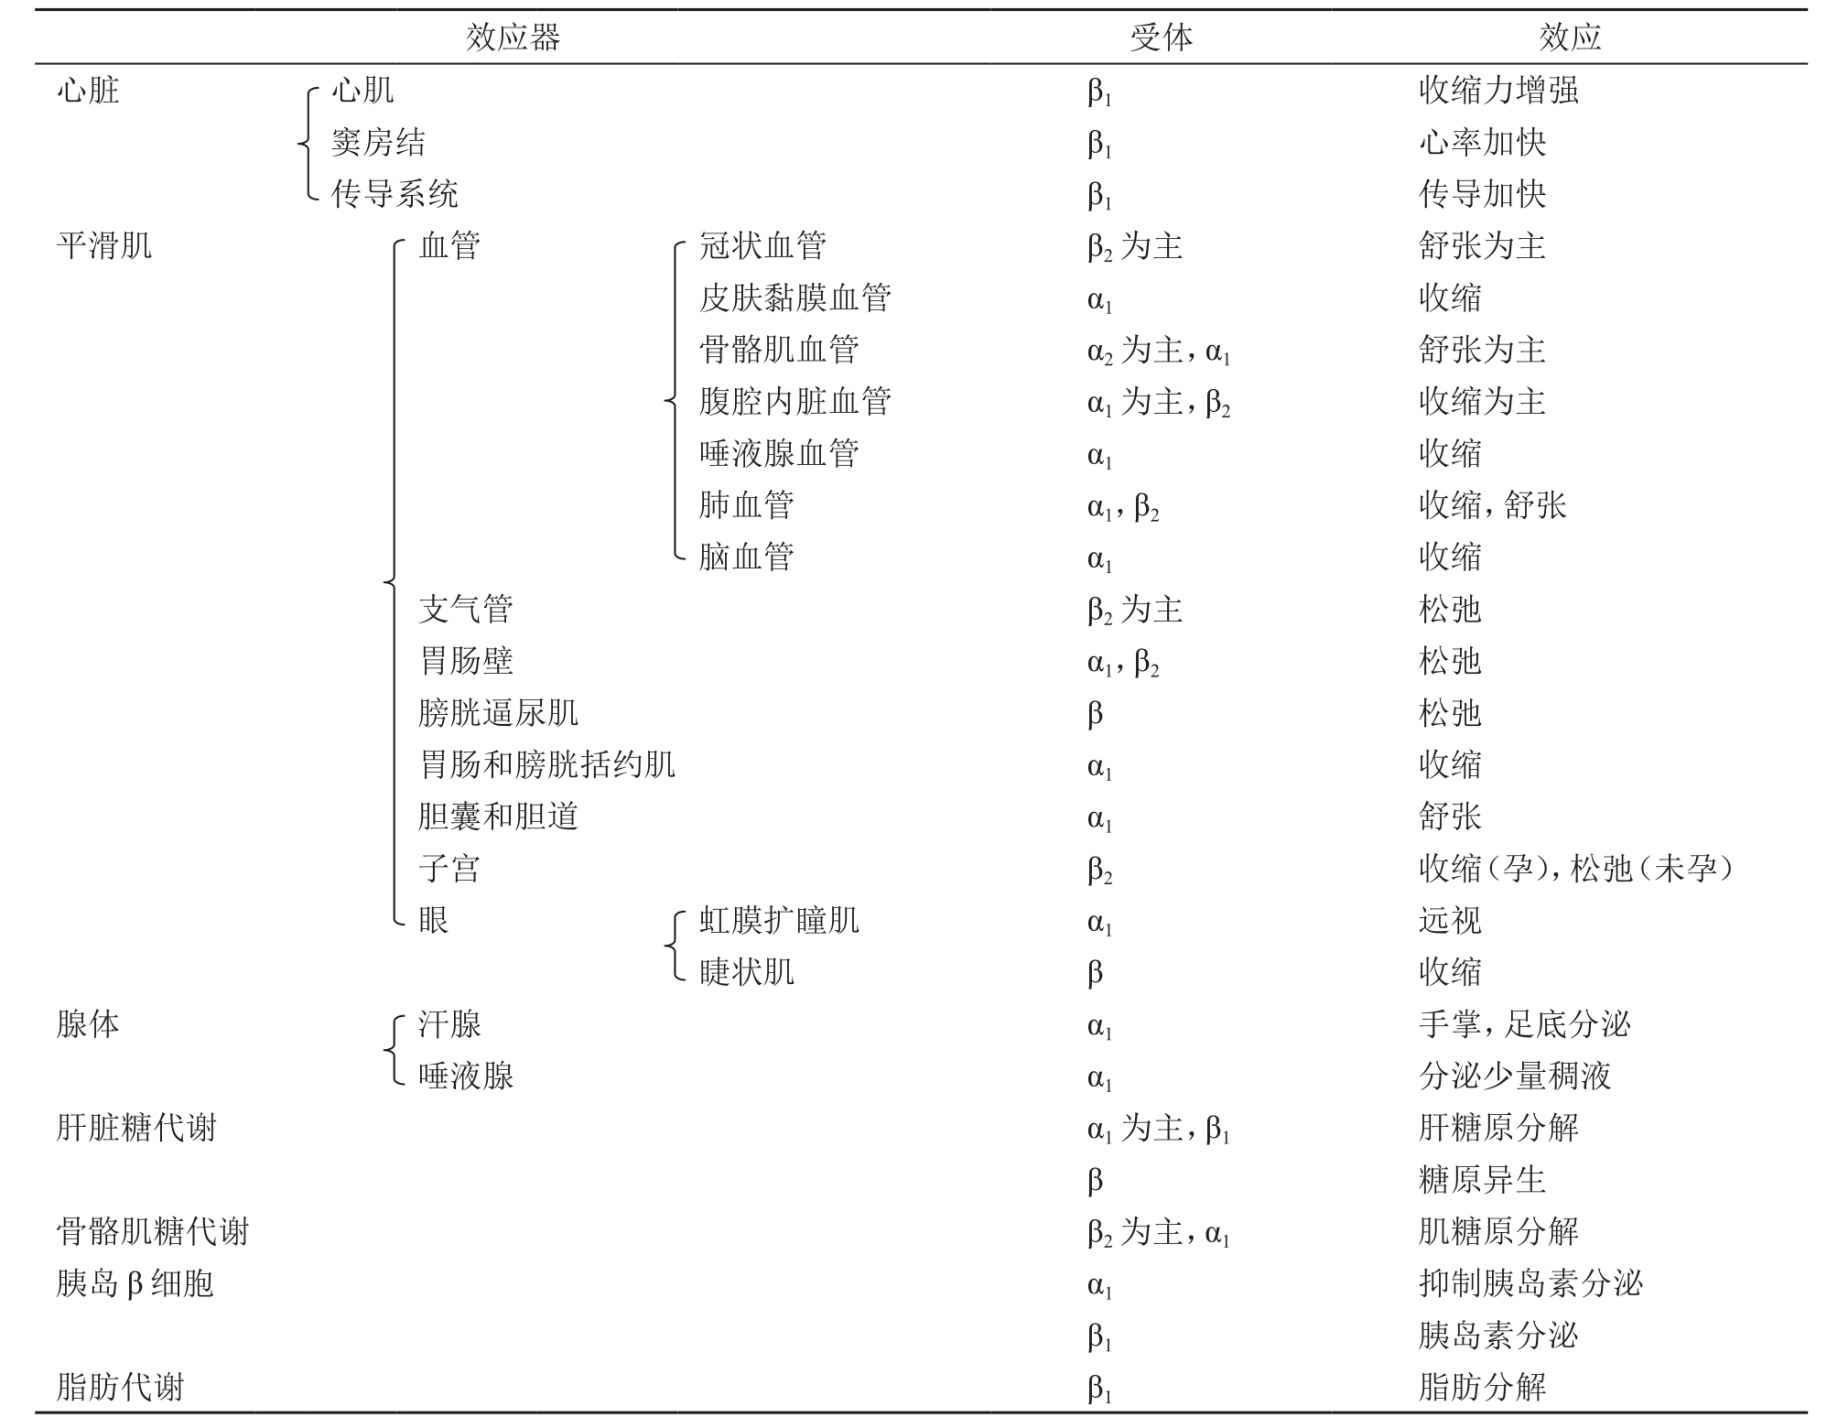
\includegraphics[width=6.64583in,height=5.1875in]{./images/Image00551.jpg}
\end{table}

\begin{table}[htbp]
\centering
\caption{拟肾上腺素药基本作用的比较}
\label{tab149-2}
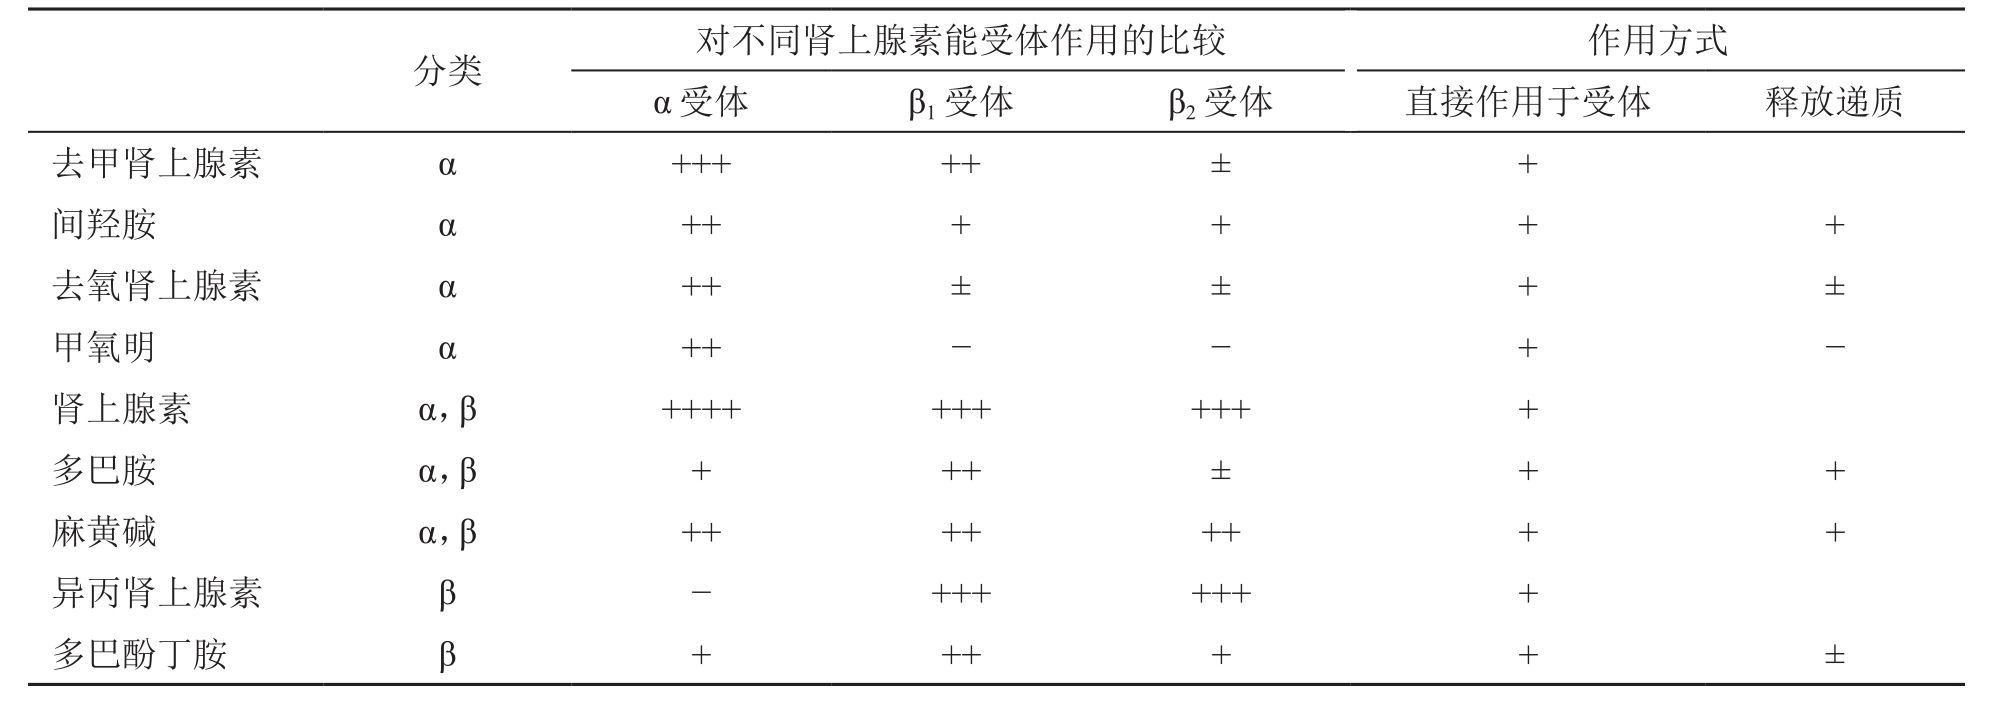
\includegraphics[width=6.65625in,height=2.35417in]{./images/Image00552.jpg}
\end{table}

\begin{table}[htbp]
\centering
\caption{常用拟肾上腺素药物主要药理作用}
\label{tab149-3}
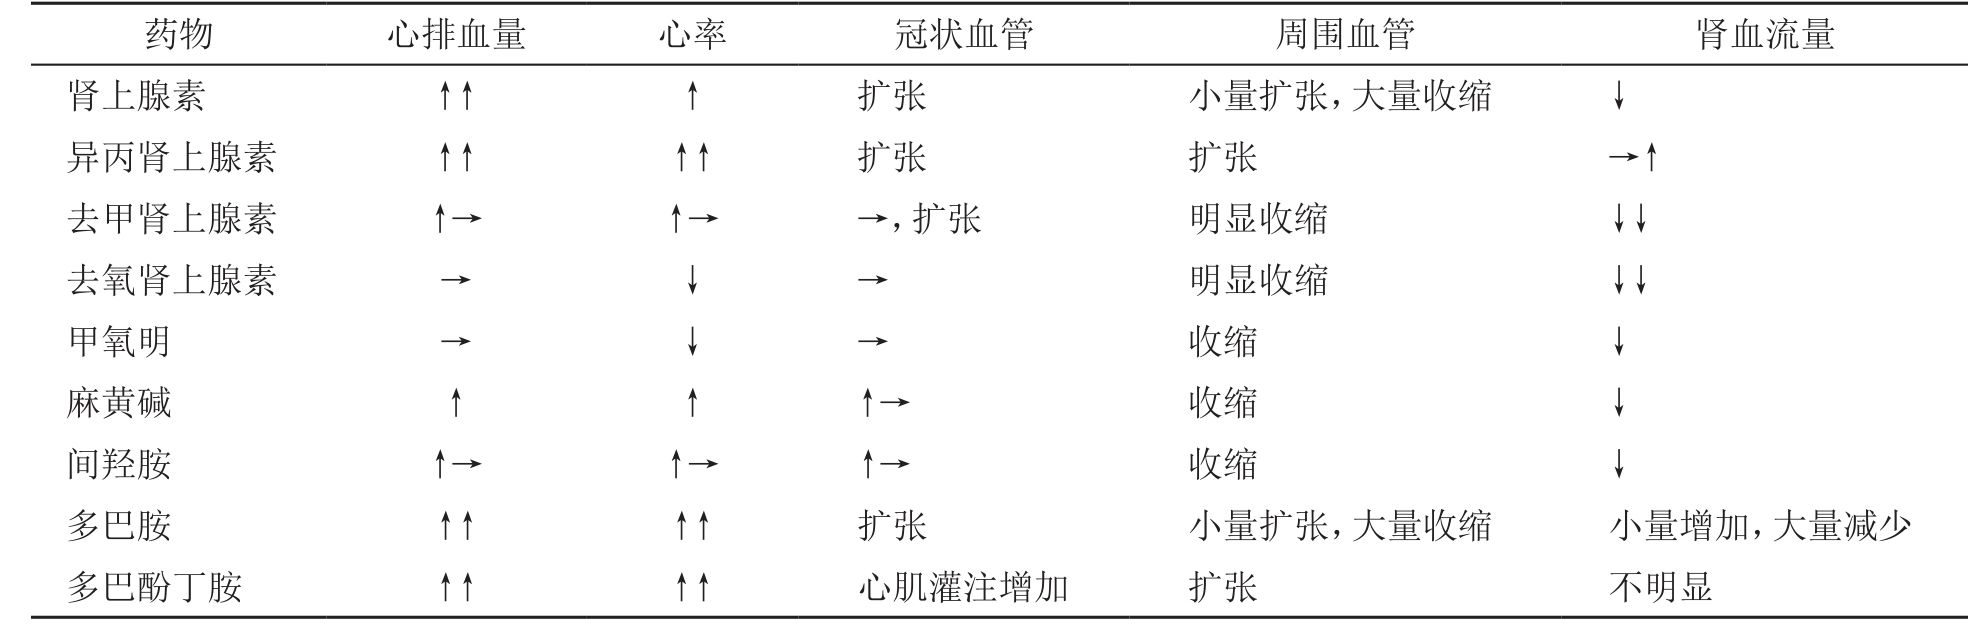
\includegraphics[width=6.60417in,height=2.125in]{./images/Image00553.jpg}
\end{table}

比较实用的分类方法是按其对不同肾上腺素能受体的选择性而分为三大类:①α受体激动药(α-adrenoceptor
agonists):主要通过激动α肾上腺素能受体而发挥作用;②α,β受体激动药(α,β-adrenoceptor
agonists):对α和β受体均能激动;③β受体激动药(β-adrenoceptor
agonists):主要通过激动β受体而发挥作用。

各种拟肾上腺素药物对肾上腺素能受体的作用方式、效能及药理作用见表\ref{tab149-2}和表\ref{tab149-3}。

\section{α受体激动药}

\subsubsection{去甲肾上腺素(noradrenaline,NA;norepinephrine,}
NE;levarterenol)

去甲肾上腺素(NA)系生物机体内源性儿茶酚胺,为肾上腺素能神经末梢释放的主要递质,也可在肾上腺髓质分泌少量。药用的是人工合成品,常用其重酒石酸盐。化学性质不稳定,见光易失效,在中性尤其在碱性溶液中迅速氧化变为粉红色乃至棕色而失效。在酸性溶液中较稳定,忌与碱性药物配伍。

\paragraph{药理与应用}

主要作用于α受体(以α\textsubscript{1}
受体为主),对心脏β\textsubscript{1}
受体作用明显较弱,对β\textsubscript{2}
受体几无作用。与肾上腺素比较,其收缩血管与升压作用较强,并反射性地引起心率减慢;兴奋心脏,扩张支气管作用较弱。临床上主要利用它的升压作用,静滴用于各种休克(但出血性休克禁用),以提高血压,保证对重要器官(如脑)的血液供应;使用时间不宜过长,否则可引起血管持续强烈收缩,使组织缺氧情况加重。应用酚妥拉明以对抗其过分强烈的血管收缩作用,常能改善休克时的组织血液供应。

\paragraph{剂量与用法}

①抗休克:在心血管急诊处理中,当血流动力学有明显改变,低血压和心源性休克时为应用NA的主要适应证。总外周阻力(SVR)降低时,用NA特别有效。情况紧急时,可用1mg稀释至20ml后静脉缓慢推注,密切注意心率和血压的变化,当血压回升后即改用静滴维持。一般用1~2mg加入5\%葡萄糖液或0.9\%氯化钠注射液100~250ml中静滴。从小剂量开始(4~10μg/min),观察反应,用输液泵调节滴速以确立和维持血压在正常低限(通常使收缩压维持在100mmHg左右),一般维持数小时,待血压平稳后改用多巴胺、间羟胺混合静滴维持血压。另外,可与肾上腺素能α受体阻滞剂合用,如NA3mg与酚妥拉明10mg合用,静滴以阻滞α受体兴奋作用,而保留β受体兴奋作用,并可对抗α受体阻滞剂的降压作用。嗜铬细胞瘤摘除后,遇到血压急剧下降时,可用0.5~1mg稀释后缓慢静注来纠正低血压,继而静滴维持血压,待循环功能稳定后,逐渐减量至停药。②治疗上消化道出血:可用4~8mg加入100ml冰盐水中,口服或由胃管灌入。

\paragraph{制剂}

注射液:每支1mg(1ml);2mg(2ml)。

\paragraph{注意事项}

①高血压、动脉硬化症及器质性心脏病患者禁用。由于可诱发妊娠末期子宫收缩,引起胎儿窒息,故晚期妊娠妇女禁用。②不良反应:主要有二:一是局部组织缺血坏死,静脉滴注时间过长、浓度过高或药液漏出血管外,可引起局部缺血坏死,如发现外漏或注射部位皮肤苍白,应更换注射部位,进行热敷,并用酚妥拉明5~10mg加入0.2\%~0.25\%普鲁卡因或利多卡因10~20ml,或生理盐水20ml内作局部浸润注射以防治组织坏死。二是急性肾功能不全:滴注时间过长或剂量过大,可使肾脏血管强烈收缩,产生少尿、无尿和肾实质损伤,故用药期间尿量至少保持在每小时25ml以上。此外,容量血管强烈收缩可引起过多静脉血回流,有加重右心负荷而导致急性右心衰竭和肺水肿的危险。③用药过程中需严密观察血压、心率、尿量,并注意随时调整滴速,切勿造成血压过高和血压的大起大落,以免脑血管意外和心泵衰竭。同时,长时间静滴后,停药时应逐渐减量,如突然停用,可因周围血管扩张或低血容量而引起血压骤降。④肾上腺皮质激素:可加强血管对NA的敏感性,减轻NA对血管壁的不良刺激,两者可混合使用。⑤三氯甲烷、氟烷或环丙烷麻醉时,使用NA可诱发心律失常甚至室颤。⑥利血平、胍乙啶、可卡因及MAO抑制剂可加强NA的升压作用;三环抗抑郁药(如丙米嗪)可使本品升压作用剧烈增加。⑦氯丙嗪等吩噻嗪类药物引起的血压下降可用NA对抗,而肾上腺素则禁用。⑧不宜与偏碱性药物如氨茶碱等配伍注射,以免失效。在碱性溶液中如与谷氨酸钠、碳酸氢钠相遇,易变紫色,并降低活性。

\subsubsection{间羟胺(metaraminol,阿拉明,Aramine)}

\paragraph{药理与应用}

间羟胺是效应较强的拟交感胺,化学性质稳定。主要作用于α受体,对β\textsubscript{1}
受体作用较弱。间羟胺可被肾上腺素能神经末梢摄取、进入囊泡,通过置换作用促使囊泡中的NA释放,故可认为间羟胺部分通过这种促进递质的释放而间接地发挥拟肾上腺素作用。本品不易被MAO破坏,故作用较持久。短时间内连续使用,可因囊泡内NA减少,使效应逐渐减弱,产生快速耐受性。本品的作用特点是收缩血管、升压作用较NA弱而持久,略增强心肌收缩力,使休克患者的心输出量增加;对心率的影响不明显,有时血压升高反射地使心率减慢,很少引起心律失常,对肾脏血管的收缩作用也较弱,较少引起少尿等不良反应。无局部刺激,供皮下注射、肌注及静注。可增加脑及冠状动脉的血流量,肌注后5分钟内血压升高,可维持1.5~4小时。静滴1~2分钟内即可显效。故目前临床上作为NA的代用品,用于各种休克早期或低血压状态以维持血压。

\paragraph{剂量与用法}

①肌注:剂量视病情而定,一般每次5~10mg,每1/2~2小时1次,小儿每次0.04~0.2mg/kg。②静注:紧急情况下可直接缓慢静注0.5~5mg,然后继以静滴。③静滴:以10~100mg加入5\%葡萄糖液或生理盐水500ml中静脉滴注,每分钟20~30滴,用量及滴速随病情而定。

\paragraph{制剂}

注射液:每支10mg(1ml)(相当于重酒石酸间羟胺18.9mg)。

\paragraph{注意事项}

①不宜与氟烷、环丙烷等提高心肌应激性的药物同时使用,以免引起心律失常。②不能与碱性药物配伍使用。③甲亢、高血压、充血性心力衰竭及糖尿病患者慎用。④连续使用既有蓄积作用,又有快速耐药性,故不宜大剂量长时间使用。⑤静注时应缓慢,同时应密切监测血压,避免引起心悸、心动过速或反射性心动过缓,静注和滴入时,均应防止漏出血管外引起局部组织缺血性坏死。⑥MAO抑制剂可加强本品的升压作用,凡10日内使用过该类药物者,不得使用本品,以免引起严重高血压。⑦降压药中甲基多巴可使间羟胺作用增强,利血平使间羟胺作用减弱,神经节阻断药如美卡拉明(美加明)等提高小动脉对α受体的敏感性,使外周血管对间羟胺的反应增强。⑧吩噻嗪类药物阻断间羟胺的α受体作用而保留其β受体兴奋作用,使血管扩张,故吩噻嗪类药物的人工冬眠血压过低时忌用间羟胺。

\subsubsection{去氧肾上腺素(苯肾上腺素,phenylephrine,新福林,neosynephrine,新辛内弗林,新交感酚)}

\paragraph{药理与应用}

主要兴奋α受体,对β\textsubscript{1}
受体仅有微弱的兴奋作用,因此,有明显的血管收缩作用,与NA作用相似,但较弱而持久,毒副作用小。可反射性地兴奋迷走神经,使心率减慢,并有短暂的散瞳作用。对心肌无兴奋作用,一般用量不致引起心律失常。临床上用于感染中毒性及过敏性休克、室上性心动过速、防治全身麻醉及腰麻时的低血压。此外,本品还能兴奋瞳孔扩大肌产生扩瞳作用,与阿托品相比,扩瞳作用较弱,维持时间短,一般不引起眼内压升高(老年人前房角狭窄者可能引起眼内压升高),用其2\%~5\%溶液滴眼,在眼底检查时可作为快速短效而不麻痹调节功能的扩瞳药。

\paragraph{剂量与用法}

①肌注:每次2~5mg,1~2小时1次;极量:每次10mg,每日50mg。小儿:每次0.1~0.25mg/kg。②静注:每次5~10mg,应缓慢。③静滴:10~20mg加入葡萄糖液100ml,滴速及剂量根据血压而定。

\paragraph{制剂}

注射液:每支10mg(1ml)。滴眼剂:为2\%~5\%溶液。

\paragraph{注意事项}

①不良反应有恶心、呕吐、头晕、四肢疼痛、反射性心动过缓等,大剂量引起期前收缩、室速等心律失常。②甲亢、高血压、动脉硬化、糖尿病、心肌病、心动过缓患者慎用。

\protect\hypertarget{text00406.html}{}{}

\section{α,β受体激动药}

\subsubsection{肾上腺素(adrenaline,AD;epinephrine,suprarenaline,副肾素,副肾碱)}

肾上腺素为正常机体肾上腺髓质分泌的内源性儿茶酚胺。临床应用的肾上腺素是从家畜(牛、羊)的肾上腺髓质中提取或用人工方法合成。皮下注射本品因能收缩血管,故吸收缓慢;肌内注射的吸收远较皮下注射为快;肌内注射作用持续约10~30分钟,皮下注射作用维持1小时左右。肾上腺素在体内的摄取与代谢途径与去甲肾上腺素相似。

\paragraph{药理与应用}

肾上腺素是具有α和β受体双重兴奋作用的儿茶酚胺。①肾上腺素对心肌的直接作用,表现为α和β受体兴奋,增强心肌的兴奋性、收缩性,增加心肌张力和收缩力,提高心输出量,加速传导,加快心率,对心室纤颤可使细颤变为粗颤,因而增加电除颤的成功率;另一方面,肾上腺素可提高胸外按压效率,由于兴奋α受体使外周血管收缩,增加了平均动脉压(MAP),提高冠状动脉和其他重要脏器的灌注压;由于β\textsubscript{1}
受体兴奋,使冠状血管扩张,心肌供血、供氧改善。故结合正确胸外按压和电除颤,能提高心脏复苏的成功率。其不利的一面是提高心肌代谢,使心肌耗氧量增加,加上心肌兴奋性提高,如剂量过大或静脉注射太快,可引起心律失常,出现期前收缩,甚至引起心室纤颤。②肾上腺素的血管效应:由于肾上腺素能兴奋α和β受体,故对血管有双重作用,使皮肤、黏膜和内脏血管收缩,同时引起冠状血管和骨骼肌血管扩张,使体内血流发生重新分配。若α受体兴奋占优势时,对冠状血管和心内膜下血管有直接收缩作用,但由于心肌兴奋性增高,代谢加强而其产物如腺苷等增多,迅速引起冠状血管和心内膜下血管扩张;β受体兴奋时,直接引起冠状血管扩张,因此,对冠状动脉来说,肾上腺素总的是导致冠脉扩张。肾上腺素主要作用于小动脉及毛细血管前括约肌,因这些小血管壁的肾上腺素能受体密度高;而静脉和大动脉的肾上腺素能受体密度低,故作用较弱。由于体内各部位血管的肾上腺素能受体的种类和密度各不相同,所以肾上腺素对各部位血管的效应也不一致,以皮肤黏膜血管收缩为最强烈;内脏血管,尤其是肾血管,也显著收缩;对脑和肺血管收缩作用十分微弱,有时由于血压升高而被动地舒张。③血压效应:在皮下注射治疗量(0.5~1mg)或低浓度静滴(每分钟滴入10μg)时,由于心脏兴奋,心输出量增加,故收缩压升高;由于骨骼肌血管舒张作用对血压的影响,抵消或超过了皮肤黏膜血管收缩作用的影响,故舒张压不变或下降;较大剂量静脉注射时,血管收缩,尤以皮肤黏膜和肾血管收缩较强,故收缩压和舒张压均升高。④支气管效应:能激动支气管平滑肌的β\textsubscript{2}
受体,发挥强大舒张作用,并能抑制肥大细胞释放过敏性物质如组胺、慢反应物质等;且能导致支气管黏膜血管收缩,降低毛细血管的通透性,消除支气管黏膜水肿,有利于保持气道通畅和改善呼吸功能。⑤代谢效应:肾上腺素能促进糖原分解,升高血糖,尚具降低外周组织对葡萄糖摄取的作用。能激活甘油三酯酶加速脂肪分解,使血液中游离脂肪酸升高。增加心肌和全身氧耗,促进异化作用,提高基础代谢率。临床主要用于抢救心脏骤停、过敏性疾患(过敏性休克)、支气管哮喘和与局部麻醉药合用及局部止血等。

\paragraph{制剂}

注射液:每支1mg(1ml)。

\paragraph{注意事项}

①治疗量可出现焦虑不安、心悸、血压升高、震颤、无力、眩晕、头痛、呕吐、四肢发冷;有时可引起心律失常,严重者可由于心室纤颤而致死。用量过大或皮下注射误入血管后,可引起血压突然上升而导致脑出血。②严重器质性心脏病、严重动脉硬化、心肌梗死、糖尿病、甲亢、心律失常、高血压、心源性哮喘、妊娠等禁用,但心脏复苏时例外。③肾上腺素不能直接加入碳酸氢钠溶液,因碱性液可使儿茶酚胺部分灭活。④胍乙啶、利血平、可卡因及丙米嗪类三环抗抑郁剂可抑制肾上腺素能神经突触前膜摄取去甲肾上腺素和肾上腺素,与肾上腺素合用时可引起严重高血压。⑤氯丙嗪等吩噻嗪类药物以及α受体阻断药等,有α受体阻断作用,当引起血压下降而需使用血管收缩药时,忌用肾上腺素。因肾上腺素的α作用被阻断而β作用可产生进一步的血管扩张,可导致严重休克。

\subsubsection{多巴胺(dopamine,3-羟酪胺,儿茶酚乙胺)}

\paragraph{药理与应用}

多巴胺具有其独特的心血管调节效应。它能兴奋α和β受体,对突触前后受体均有兴奋作用,并能兴奋多巴胺能受体。其作用的多样性与多巴胺分子构型易变、能适应多种受体结构有关。本品的作用与剂量有密切相关,其作用随剂量而异,且有明显的个体差异。在0.5~2μg/(kg•min)剂量时,兴奋多巴胺受体,外周血管阻力降低,血压降低,肾血流和Na\textsuperscript{+}
排出增加;2~4μg/(kg•min)时,兴奋β\textsubscript{1}
受体,心输出量增加;5μg/(kg•min)时,α受体开始激活,血管收缩;至10μg/(kg•min)时,则α受体兴奋作用显著,导致全部血管床动、静脉收缩,血压升高,肾动脉也开始收缩,尿量逐渐减少;当剂量大于20μg/(kg•min)时,α受体的强烈兴奋可逆转其肾、肠系膜血管的扩张作用,而导致肾、肠系膜血管收缩,血流量减少。因此,临床上使用本药时要根据病情、血压、尿量等情况,调节其浓度和剂量。

小剂量多巴胺兴奋肾、脑、冠状动脉和肠系膜血管壁上的多巴胺能受体,使其扩张、血流增加。小剂量多巴胺有增加肾血流量,并直接作用于肾小管使其对钠的重吸收受到抑制,还能抑制醛固酮的生物合成,起排钠、利尿作用。多巴胺通过对心肌β\textsubscript{1}
受体的兴奋而起正性肌力作用,但较去甲肾上腺素和异丙肾上腺素缓和。多巴胺对心率和心律的影响与剂量有关,小剂量心率不增快,大剂量则可使心率加快,甚至引起室性或室上性心动过速,但其作用较去甲肾上腺素和异丙肾上腺素为弱;血压升高,有时可反射性地引起心率减慢,且有个体差异。

临床上用于治疗各种低血压和休克,包括中毒性休克、心源性休克、出血性休克、创伤性休克等,对休克伴有肾功能不全、心排出量降低、周围血管阻力增高、微循环灌注不良而已基本补足血容量的患者更为有益。此外,长时间机械呼吸和PEEP治疗可反射性地引起肾血管收缩,肾素分泌增加,肾皮质血流量减少,周围血管阻力增加,右心回流量减少,钠、水潴留;多巴胺通过兴奋肾内多巴胺受体能解除肾血管收缩,使肾皮质血流量明显增加,肾小球滤过率、尿量及排钠量增多,对长时间机械呼吸和PEEP引起的生理功能紊乱,有良好的预防和治疗作用。既往认为多巴胺与利尿剂合用对治疗急性肾衰竭有益。充血性心力衰竭用洋地黄治疗无效,或已产生中毒症状而心衰未能控制者,试用多巴胺常可取得明显疗效。

\paragraph{剂量与用法}

目前临床上对低血压和休克的治疗,常首选多巴胺静滴,以发挥多巴胺强心、收缩外周血管,提高血压而同时扩张肾及肠系膜血管、增加钠和尿排量的特点。宜及早使用,开始时应用剂量为2~5μg/(kg•min),观察反应,并不断调整滴速,以求最小有效浓度和剂量。情况紧急时,也可用20mg稀释到20ml液体中缓慢静注。

\paragraph{制剂}

注射液:每支20mg(2ml)。

\paragraph{注意事项}

①不良反应一般较轻,偶见恶心、呕吐,剂量过大或滴注太快可出现心动过速和心律失常等,一旦出现应减量或停药,即可消失。②多巴胺系酸性药物,不能加入碳酸氢钠和其他碱性药液中静滴,否则会失去活性。③使用前应补充血容量及纠正酸中毒。④单胺氧化酶抑制剂能使神经元内去甲肾上腺素及多巴胺积聚,同时多巴胺约75\%由单胺氧化酶代谢灭活,故单胺氧化酶抑制剂可使多巴胺的作用时间及强度增加,甚至可引起高血压危象。合用时多巴胺不能超过常用量的1/3,且静滴要缓慢。(呋喃唑酮(痢特灵)的代谢产物亦有单胺氧化酶抑制作用,治疗中毒型痢疾时,须注意。⑤嗜铬细胞瘤或心律失常未纠正者禁用。⑥多巴胺仅供静脉内应用,如漏至皮下或外溢,可引起皮肤组织坏死。一旦发生,要与去甲肾上腺素外溢同样处理。

\subsubsection{麻黄碱(麻黄素,ephedrine,ephetonin)}

\paragraph{药理与应用}

麻黄碱能直接作用于α、β受体,发挥拟肾上腺素作用;也能促使肾上腺素能神经末梢释放递质,间接地发挥拟肾上腺素作用。与肾上腺素比较麻黄碱具有下列特点:①性质稳定,口服有效;②拟肾上腺素作用弱而持久;③可通过血脑屏障进入脑脊液,故中枢兴奋作用较显著,较大剂量可兴奋大脑和皮质下中枢,引起精神兴奋、不安和失眠等;④易产生快速耐受性(tachyphylaxis),也称脱敏(desensitization),停药数小时后,可以恢复。麻黄碱兴奋心脏使心肌收缩力增强,心输出量增加,对皮肤黏膜和内脏血管呈收缩作用,但冠脉、脑血管和骨骼肌血流量增加;其升压作用缓慢而持久,松弛支气管平滑肌的作用比肾上腺素弱。临床用于支气管哮喘、过敏性反应(荨麻疹、血管神经性水肿的皮肤黏膜肿胀)、鼻黏膜肿胀、脊髓麻醉前预防血压下降。

\paragraph{剂量与用法}

口服,每次25mg,每日3次;皮下或肌内注射,每次15~30mg。极量:每次60mg,每日150mg,口服、皮下或肌内注射。

\paragraph{制剂}

片剂:每片15mg;25mg;30mg。注射液:每支30mg(1ml),50mg(1ml)。

\paragraph{注意事项}

①用量过大时可引起兴奋、不安、焦虑、失眠、心悸、出汗等不良反应。②与镇静药物合用,可减少不良反应。③甲亢、高血压、动脉硬化、心绞痛等患者忌用。

\protect\hypertarget{text00407.html}{}{}

\section{β受体激动药}

\subsubsection{异丙肾上腺素(isoprenaline,喘息定,治喘灵,isoproterenol)}

\paragraph{药理与应用}

为非选择性肾上腺素β受体激动剂,对β\textsubscript{1} 和β\textsubscript{2}
受体均有强大的激动作用,对α受体几无作用。主要作用如下:①作用于心脏β\textsubscript{1}
受体,加强心肌收缩力,使心率加快、传导加速,心输出量和心肌耗氧量增加。②作用于血管平滑肌β\textsubscript{2}
受体,使骨骼肌血管明显舒张,肾、肠系膜血管及冠状动脉亦不同程度舒张,血管总外周阻力降低。其心血管作用导致收缩压升高,舒张压下降,脉压变大。③作用于支气管平滑肌β\textsubscript{2}
受体,使支气管平滑肌松弛。本品解除支气管痉挛作用比肾上腺素强,但对支气管黏膜血管无收缩作用,故消除黏膜水肿的作用不及肾上腺素。④促进糖原和脂肪分解,增加组织耗氧量。临床主要用于支气管哮喘、中毒性休克及房室传导阻滞等。

\paragraph{剂量与用法}

①治疗支气管哮喘急性发作:成人一般用10~15mg舌下含服,1日3次;极量:一次20mg,一日60mg。0.25\%气雾剂吸入:常用量每次0.1~0.4mg,极量一次0.4mg,一日2.4mg。重复使用的间隔时间不应少于2小时。②房室传导阻滞:二度者采用舌下含片,每次10mg,每4小时1次;三度者如心率低于40次/分时,可用0.5~1mg加入5\%葡萄糖液250~500ml内静滴,开始宜慢,根据心率和心律反应来确定最低有效剂量,滴速一般为2~20μg/min。③抗休克:对血容量已补足,心搏出量较低及CVP较高的感染中毒性休克最为适用。以0.5~1mg加入5\%葡萄糖液250ml内静滴,根据心率调整滴速,使收缩压维持在90mmHg、脉压在20mmHg以上、心率120次/分以下。

\paragraph{制剂}

片剂:每片10mg,纸片:每片5mg。注射液:每支1mg(2ml)。气雾剂:0.25\%
10ml,0.25\% 20ml,0.5\% 10ml。

\paragraph{注意事项}

①异丙肾上腺素在碱性溶液中易迅速破坏,故不宜与碱性药配伍;口服易被胃内的酸破坏,故不宜口服。临床用舌下、吸入和静脉内给药。②不良反应有恶心、头痛、眩晕、震颤等,也可引起心动过速、室性心律失常等,严重者可致心室纤颤。③尽量避免与肾上腺素同用,以免引起致死性心律失常。包括洋地黄中毒在内的各种快速性心律失常和低钾血症时,禁用异丙肾上腺素。④钾盐引起血钾增高,增强本品对心肌的兴奋作用,易致心律失常,禁止合用。⑤心肌炎、心绞痛、心肌梗死、甲亢和心动过速者应禁用。

\subsubsection{多巴酚丁胺(dobutamine,杜丁胺,dobutrex, inotrex)}

\paragraph{药理与应用}

为选择性心脏β\textsubscript{1} 受体激动剂,对β\textsubscript{2}
受体和α受体作用较弱,对多巴胺受体则无作用。本品增强心肌收缩力比加快心率明显是其优点,并能加快房室传导。治疗剂量能增加心肌收缩力和心输出量,而对心率影响不大,耗氧量增加亦不多。临床对心肌梗死后或心脏手术时心排血量低的休克患者有较好疗效,优于异丙肾上腺素,较为安全。用于心排血量低和心率慢的心力衰竭患者,其改善左心室功能的作用优于多巴胺。

\paragraph{用法}

静滴:一般用40~100mg加入5\%葡萄糖液250ml中,以2.5~10μg/(kg•min)的剂量滴入。

\paragraph{制剂}

注射液:每支20mg(2ml);200mg(2ml)。盐酸多巴酚丁胺葡萄糖注射液:①250ml:盐酸多巴酚丁胺0.125g与葡萄糖25g;②250ml:盐酸多巴酚丁胺0.25g与葡萄糖25g;③250ml:盐酸多巴酚丁胺0.5g与葡萄糖25g。

\paragraph{注意事项}

①本品与其他β受体兴奋剂一样,也可引起心动过速和室性期前收缩等心律失常;尤其当剂量超过20μg/(kg•min)时,更应注意观察。如出现收缩压增高10~20mmHg以上或心率加快10~15次/分以上,应认为过量,宜减量或暂停给药。剂量超过20μg/(kg•min),可使心率增加10\%,超过40μg/(kg•min)时,可能会导致中毒。此外,本品连用3天后可因β受体下调而逐渐失效。②可能有头痛、恶心、心悸、气急等不良反应,减少剂量后即可消失。③因能促进房室传导,故快速心房颤动患者禁用。④梗阻型肥厚性心肌病患者禁用。

\protect\hypertarget{text00408.html}{}{}

\hypertarget{text00408.htmlux5cux23CHP17-2-4}{}
参 考 文 献

陈新谦,金有豫,汤光.新编药物学.第17版.北京:人民卫生出版社,2011

\protect\hypertarget{text00409.html}{}{}

\chapter{抗高血压药}

高血压(hypertension)是以体循环动脉压升高、外周小动脉阻力增高同时伴有不同程度的心排血量和血容量增加为主要表现的临床综合征。高血压可分为原发性和继发性,其中原发性者占90\%~95\%,继发性者占5\%~10\%。原发性高血压又称高血压病。

高血压是最常见的慢性病,也是心脑血管病最主要的危险因素,其脑卒中、心肌梗死、心力衰竭及慢性肾脏病等主要并发症,不仅致残、致死率高,而且严重消耗医疗和社会资源,给家庭和国家造成沉重负担。国内外的实践证明,高血压是可以预防和控制的疾病,降低高血压患者的血压水平,可明显减少脑卒中及心脏病事件,显著改善患者的生存质量,有效降低疾病负担。

为进一步加强我国高血压的人群防治工作,提高防治效果,中华人民共和国卫生部疾病预防控制局委托国家心血管病中心和高血压联盟(中国)组织有关专家对2005年《中国高血压防治指南》进行修订,于2010年底完稿,颁布了《2010中国高血压防治指南》。

\section{2010中国高血压防治指南中的几个要点}

《2010中国高血压防治指南》坚持预防为主,防治结合的方针,提出符合我国人群特点的防治策略,从控制危险因素、早诊早治和患者规范化管理入手,加强对公众的健康教育和高血压的社区防治,努力提高人群高血压的知晓率、治疗率和控制率。指南保留了以往指南的合理部分,更新了部分观念,增加了儿童和青少年高血压、继发性高血压等“特殊人群”章节。指出应对高血压患者全面检查评估,根据患者心血管总危险度决定治疗措施。强调高血压患者改变不良生活方式的必要性;强调长期平稳控制血压的重要性;强调降低高血压患者血压水平是减少心脑血管病的关键。

\subsubsection{我国人群高血压流行情况}

我国人群50年来高血压患病率呈明显上升趋势。目前我国约有2亿高血压患者,每10个成年人中有2人患高血压。我国人群高血压流行有两个比较显著的特点:从南方到北方高血压患病率递增;不同民族之间高血压患病率存在一些差异。高钠、低钾膳食是我国大多数高血压患者发病的主要危险因素之一。超重和肥胖将成为我国高血压患病率增长的又一重要危险因素。我国高血压患者总体的知晓率、治疗率和控制率明显较低,分别低于50\%、40\%和10\%。

\subsubsection{高血压与心血管病风险}

高血压是一种“心血管综合征”。无论采用哪种测量方法,诊室血压、动态血压或家庭血压,血压水平与脑卒中、冠心病事件的风险均呈连续、独立、直接的正相关。与舒张压(DBP)相比,收缩压(SBP)与心血管风险的关系更为密切。目前,冠心病事件有上升趋势,但脑卒中仍是我国高血压人群最主要的并发症。

\subsubsection{高血压患者诊断性评估}

高血压患者诊断性评估的内容包括以下三方面:①确定血压水平及其他心血管危险因素。②判断高血压的病因,明确有无继发性高血压。③寻找靶器官损害以及相关临床情况。从而作出高血压病因的鉴别诊断和评估患者的心血管风险度。以指导诊断与治疗。

\hypertarget{text00409.htmlux5cux23CHP17-3-1-3-1}{}
(一) 病史

应全面详细了解患者病史,包括以下内容:

\hypertarget{text00409.htmlux5cux23CHP17-3-1-3-1-1}{}
(1) 家族史:

询问患者有无高血压、糖尿病、血脂异常、冠心病、脑卒中或肾脏病的家族史。

\hypertarget{text00409.htmlux5cux23CHP17-3-1-3-1-2}{}
(2) 病程:

患高血压的时间,血压最高水平,是否接受过降压治疗及其疗效与不良反应。

\hypertarget{text00409.htmlux5cux23CHP17-3-1-3-1-3}{}
(3) 症状及既往史:

目前及既往有无冠心病、心力衰竭、脑血管病、外周血管病、糖尿病、痛风、血脂异常、支气管哮喘、睡眠呼吸暂停综合征、性功能异常和肾脏疾病等症状及治疗情况。

\hypertarget{text00409.htmlux5cux23CHP17-3-1-3-1-4}{}
(4) 有无提示继发性高血压的症状:

例如肾炎史或贫血史,提示肾实质性高血压;有无肌无力、发作性软瘫等低血钾表现,提示原发性醛固酮增多症;有无阵发性头痛、心悸、多汗等提示嗜铬细胞瘤。

\hypertarget{text00409.htmlux5cux23CHP17-3-1-3-1-5}{}
(5) 生活方式:

膳食脂肪、盐、酒摄入量,吸烟支数,体力活动量以及体重变化等情况。

\hypertarget{text00409.htmlux5cux23CHP17-3-1-3-1-6}{}
(6) 药物引起的高血压:

是否服用使血压升高的药物,例如口服避孕药、生胃酮、麻黄碱类滴鼻药、可卡因、安非他明、类固醇、非甾体类抗炎药、促红细胞生长素、环孢素以及中药甘草等。

\hypertarget{text00409.htmlux5cux23CHP17-3-1-3-1-7}{}
(7) 心理社会因素:

包括家庭情况、工作环境、文化程度及有无精神创伤史。

\hypertarget{text00409.htmlux5cux23CHP17-3-1-3-2}{}
(二) 体格检查

仔细地体格检查有助于发现继发性高血压线索和靶器官损害情况,体格检查包括:正确测量血压和心率,必要时测量立、卧位血压和四肢血压;测量BMI、腰围及臀围;观察有无库欣面容、神经纤维瘤性皮肤斑、甲状腺功能亢进性突眼征或下肢水肿;听诊颈动脉、胸主动脉、腹部动脉和股动脉有无杂音;触诊甲状腺;全面的心肺检查;检查腹部有无肾脏增大(多囊肾)或肿块;检查四肢动脉搏动和神经系统体征。

\hypertarget{text00409.htmlux5cux23CHP17-3-1-3-3}{}
(三) 实验室检查

\paragraph{基本项目}

血液生化(钾、空腹血糖、总胆固醇、甘油三酯、高密度脂蛋白胆固醇、低密度脂蛋白胆固醇和尿酸、肌酐);全血细胞计数、血红蛋白和血细胞比容;尿液分析(蛋白、糖和尿沉渣镜检);心电图。

\paragraph{推荐项目}

24小时动态血压监测、超声心动图、颈动脉超声、餐后2小时血糖(当空腹血糖≥6.1mmol/L时测定)、血同型半胱氨酸、尿白蛋白定量(糖尿病患者必查项目)、尿蛋白定量(用于尿常规检查蛋白阳性者)、眼底、胸部X线检查、脉搏波传导速度以及踝臂血压指数等。

\paragraph{选择项目}

对怀疑为继发性高血压患者,根据需要可以分别选择以下检查项目:血浆肾素活性、血和尿醛固酮、血和尿皮质醇、血游离甲氧基肾上腺素及甲氧基去甲肾上腺素、血和尿儿茶酚胺、动脉造影、肾和肾上腺超声、CT或磁共振成像(MRI)、睡眠呼吸监测等。对有并发症的高血压患者,进行相应的脑功能、心功能和肾功能检查。

\hypertarget{text00409.htmlux5cux23CHP17-3-1-3-4}{}
(四) 血压测量

血压测量是评估血压水平
、诊断高血压以及观察降压疗效的主要手段。目前,在临床和人群防治工作中,主要采用诊室血压、动态血压以及家庭血压3种方法。诊室血压由医护人员在诊室按统一规范进行测量,目前尚是评估血压水平和临床诊断高血压并进行分级的标准方法和主要依据。动态血压监测则通常由自动的血压测量仪器完成,测量次数较多,无测量者误差,可避免白大衣效应,并可测量夜间睡眠期间的血压。因此,既可更准确地测量血压,也可评估血压短时变异和昼夜节律。家庭血压监测通常由被测量者自我完成,这时又称自测血压或家庭自测血压。但也可由家庭成员等协助完成。因为测量在熟悉的家庭环境中进行,因而,也可以避免白大衣效应。家庭血压监测还可用于评估数日、数周甚至数月、数年血压的长期变异或降压治疗效应,而且有助于增强患者的参与意识,改善患者的治疗依从性。

\paragraph{诊室血压}

具体方法和要求如下:①选择符合计量标准的水银柱血压计,或者经过验证(BHS、AAMI和ESH)的电子血压计。②使用大小合适的气囊袖带,气囊至少应包裹80\%上臂。大多数成年人的臂围25~35cm,可使用气囊长22~26cm、宽12~14cm的标准规格袖带(目前国内商品水银柱血压计的气囊的规格:长22cm,宽12cm)。肥胖者或臂围大者应使用大规格气囊袖带;儿童应使用小规格气囊袖带。③测血压前,受试者应至少坐位安静休息5分钟,30分钟内禁止吸烟,饮咖啡、茶和排空膀胱。④受试者取坐位,最好坐靠背椅,裸露上臂,上臂与心脏处在同一水平。如果怀疑外周血管病,首次就诊时应测量左、右臂血压,以后通常测量较高读数一侧的上臂血压,必要时加测下肢血压,选择宽度>
16cm的袖带。特殊情况下可以取卧位或站立位。老年人、糖尿病患者及出现直立性低血压情况者,应加测站立位血压。站立位血压应在卧位改为站立位后1分钟和5分钟时测量。⑤将袖带紧贴缚在被测者的上臂,袖带的下缘应在肘弯上2.5cm。将听诊器探头置于肱动脉搏动处。⑥使用水银柱血压计测压时,快速充气,使气囊内压力达到桡动脉搏动消失后,再升高30mmHg,然后以恒定的速率(2~6mmHg/秒)缓慢放气。心率缓慢者,放气速率应更慢些。获得DBP读数后,快速放气至零。⑦在放气过程中仔细听取柯氏音,观察柯氏音第1时相(第一音)和第V时相(消失音)水银柱凸面的垂直高度。SBP读数取柯氏音第l时相,DBP读数取柯氏音第V时相。12岁以下儿童、妊娠妇女、严重贫血、甲状腺功能亢进、主动脉瓣关闭不全及柯氏音不消失者,可以柯氏音第Ⅳ时相(变音)为DBP。⑧血压单位在临床使用时采用毫米汞柱(mmHg),在我国正式出版物中注明毫米汞柱与千帕斯卡(kPa)的换算关系,1mmHg
=
0.133kPa。⑨应间隔1~2分钟重复测量,取2次读数的平均值记录。如果SBP或DBP的2次读数相差5mmHg以上,应再次测量,取3次读数的平均值记录。⑩使用水银柱血压计测压读取血压数值时,末位数值只能为0、2、4、6、8,不能出现l、3、5、7、9,并应注意避免末位数偏好。

\paragraph{动态血压}

具体使用方法和指征如下:①使用经BHS、AAMI和ESH方案验证的动态血压监测仪,并每年至少1次与水银柱血压计进行读数校准,采用Y或T型管与袖带连通,两者的血压平均读数相差应<
5mmHg。②测压间隔时间可选择15分钟、20分钟或30分钟。通常夜间测压间隔时间可适当延长至30分钟。血压读数应达到应测次数的80\%以上。最好每个小时有至少1个血压读数。③目前动态血压监测的常用指标是24小时、白天(清醒活动)和夜间(睡眠)的平均SBP与DBP水平,夜间血压下降百分率以及清晨时段血压的升高幅度(晨峰)。24小时、白天与夜间血压的平均值反映不同时段血压的总体水平,是目前采用24小时动态血压诊断高血压的主要依据,其诊断标准包括:24小时≥130/80mmHg,白天≥135/85mmHg,夜间≥120/70mmHg。夜间血压下降百分率:(白天平均值−夜间平均值)/白天平均值。10\%~20\%:杓型;<
10\%:非杓型。SBP与DBP不一致时,以SBP为准。血压晨峰:起床后2小时内的SBP平均值−夜间睡眠时SBP最低值(包括最低值在内1小时的平均值),≥35mmHg为晨峰血压增高。④动态血压监测也可用于评估降压疗效。主要观察24小时、白天和夜间的平均SBP与DBP是否达到治疗目标,即24小时血压<
130/80mmHg,白天血压< 135/85mmHg,且夜间血压<
120/70mmHg。⑤动态血压监测可诊断白大衣性高血压,发现隐蔽性高血压,检查顽固难治性高血压的原因,评估血压升高程度、短时变异和昼夜节律等。随着其价格的下降,动态血压监测将在临床工作中更广泛应用。

\paragraph{家庭血压}

家庭血压监测需要选择合适的血压测量仪器,并进行血压测量知识与技能培训:①使用经过验证的上臂式全自动或半自动电子血压计(BHS、AAMl和
ESH)。②家庭血压值一般低于诊室血压值,高血压的诊断标准为≥135/85mmHg,与诊室血压140/90mmHg相对应。③测量方案:目前还没有一致方案。一般情况建议,每天早晨和晚上测量血压,每次测2~3遍,取平均值;血压控制平稳者,可每周只测1天血压。对初诊高血压或血压不稳定的高血压患者,建议连续家庭测量血压7天(至少3天),每天早晚各1次,每次测量2~3遍,取后6天血压平均值作为参考值。④家庭血压适用于:一般高血压患者的血压监测,白大衣高血压识别,难治性高血压的鉴别,评价长时血压变异,辅助降压疗效评价,预测心血管风险及评估预后等。⑤最好能够详细记录每次测量血压的日期、时间以及所有血压读数,而不是只记录平均值。应尽可能向医生提供完整的血压记录。⑥家庭血压监测是观察数日、数周甚至数月、数年间长期变异情况的可行方法,未来通过无线通讯与互联网为基础的远程控制系统将可实现血压的实时、数字化监测。⑦对于精神高度焦虑患者,不建议自测血压。

\hypertarget{text00409.htmlux5cux23CHP17-3-1-3-5}{}
(五) 评估靶器官损害

高血压患者靶器官损害(心、脑、肾、血管等)的识别,对于评估患者心血管风险,早期积极治疗具有重要意义。从患高血压到最终发生心血管事件的整个疾病过程中,亚临床靶器官损害是极其重要的中间环节。采用相对简便、花费较少、易于推广的检查手段,在高血压患者中检出无症状性亚临床靶器官损害是高血压诊断评估的重要内容。

\paragraph{心脏}

心电图检查可以发现左心室肥厚、心肌缺血、心脏传导阻滞或心律失常。近年来有报道,aVL导联R波电压与左心室重量指数密切相关,甚至在高血压不伴有心电图左心室肥厚时,也可以预测心血管事件的发生。胸部X线检查可以了解心脏轮廓、大动脉及肺循环情况。超声心动图在诊断左心室肥厚和舒张期心力衰竭方面优于心电图。必要时采用其他诊断方法:心脏MRI和磁共振血管造影(MRA),计算机断层扫描血管造影(CTA),心脏核素显像,运动试验或冠状动脉造影等。

\paragraph{血管}

颈动脉内中膜厚度(IMT)和粥样斑块可独立于血压水平预测心血管事件。大动脉僵硬度增加预测并评估心血管风险的证据日益增多。多项研究证实,脉搏波传导速度(PWV)增快是心血管事件的独立预测因素。踝/臂血压指数(ABI)能有效筛查外周动脉疾病,评估心血管风险。

\paragraph{肾脏}

肾脏损害主要根据血清肌酐升高,估算的肾小球滤过率(eGFR)降低或尿白蛋白排出量(UAE)增加。微量白蛋白尿已被证实是心血管事件的独立预测因素。高血压患者尤其合并糖尿病的患者应定期检查尿白蛋白排出量,24小时尿白蛋白排出量或晨尿白蛋白/肌酐比值为最佳,随机尿白蛋白/肌酐比值也可接受。eGFR是一项判断肾脏功能的简便而且敏感的指标,可采用“肾脏病膳食改善试验(MDRD)”公式,或者我国学者提出的MDRD改良公式来计算。eGFR降低与心血管事件发生之间存在着强相关性。血清尿酸水平增高,对心血管风险可能也有一定预测价值。

\paragraph{眼底}

视网膜动脉病变可反映小血管病变情况。常规检眼镜检查的高血压眼底改变,按Keith-Wagener和Backe四级分类法,3级或4级高血压眼底对判断预后有价值。高分辨率眼底成像系统有望成为检查眼底小血管病变的工具。

\paragraph{脑}

头颅MRI、MRA或CTA有助于发现腔隙性病灶或脑血管狭窄、钙化和斑块病变。经颅多普勒超声对诊断脑血管痉挛、狭窄或闭塞有一定帮助。目前认知功能的筛查评估主要采用简易精神状态量表。

\subsubsection{高血压分类与分层}

\hypertarget{text00409.htmlux5cux23CHP17-3-1-4-1}{}
(一) 按血压水平分类

目前我国采用正常血压(SBP < 120mmHg和DBP <80mmHg)、正常高值血压{[}SBP
120~139mmHg和(或)DBP
80~89mmHg{]}和高血压{[}SBP≥140mmHg和(或)DBP≥90mmHg{]}进行血压水平分类。以上分类适用于18岁以上的男、女性成年人。

高血压定义为:在未使用降压药物的情况下,非同日3次测量血压,SBP≥140mmHg和(或)DBP≥90mmHg。SBP≥140mmHg和DBP
<
90mmHg为单纯性收缩期高血压。患者既往有高血压史,目前正在使用降压药物,血压虽然低于140/90mmHg,也诊断为高血压。根据血压升高水平,又进一步将高血压分为1级、2级和3级(表\ref{tab150-1})。\footnote{当SBP和DBP分属于不同级别时,以较高的分级为准}

\begin{table}[htbp]
\centering
\caption{血压水平分类和定义}
\label{tab150-1}
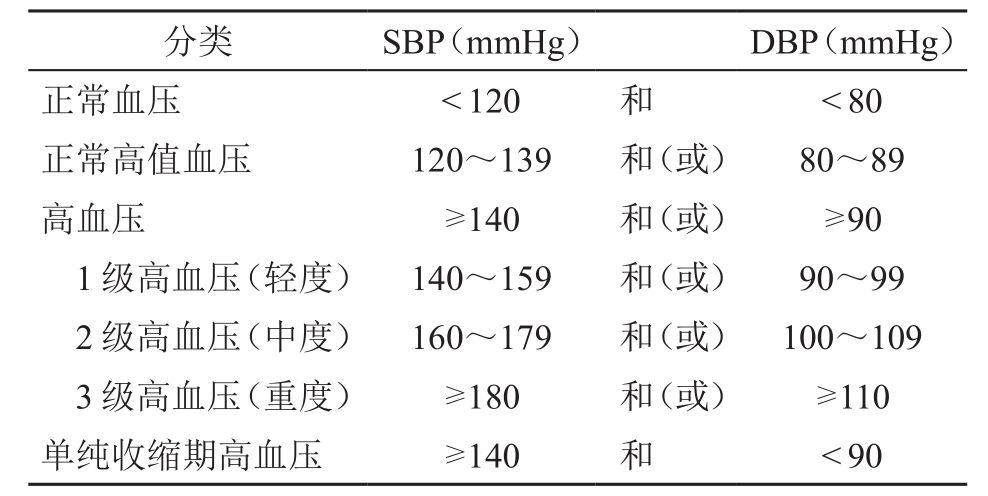
\includegraphics[width=3.28125in,height=1.64583in]{./images/Image00554.jpg}
\end{table}



\hypertarget{text00409.htmlux5cux23CHP17-3-1-4-2}{}
(二) 按心血管风险分层

脑卒中
、心肌梗死等严重心脑血管事件是否发生、何时发生难以预测,但发生心脑血管事件的风险水平不仅可以评估,也应该评估。虽然高血压及血压水平是影响心血管事件发生和预后的独立危险因素,但是并非唯一决定因素。大部分高血压患者还有血压升高以外的心血管危险因素。因此,高血压患者的诊断和治疗不能只根据血压水平,必须对患者进行心血管风险的评估并分层。高血压患者的心血管风险分层,有利于确定启动降压治疗的时机,有利于采用优化的降压治疗方案,有利于确立合适的血压控制目标。有利于实施危险因素的综合管理。

2010年指南仍采用2005年指南的分层原则和基本内容,将高血压患者按心血管风险水平分为低危、中危、高危和很高危4个层次(表\ref{tab150-2})。根据以往我国高血压防治指南实施情况和有关研究进展,对影响风险分层的内容作了部分修改(表\ref{tab150-3}\footnote{TC:总胆固醇;LDL-C:低密度脂蛋白胆固醇;HDL-C:高密度脂蛋白胆固醇;BMI:体质指数;LVMI:左心室质量指数;IMT:颈动脉内中膜厚度:eGFR:估算的肾小球滤过率})。将糖耐量受损和(或)空腹血糖异常列为影响分层的心血管危险因素;将判定腹型肥胖的腰围标准改为:男性≥90cm,女性≥85cm;将eGFR
< 60ml(/min•1.73m\textsuperscript{2}
)、颈-股动脉脉搏波速度≥12m/s和踝/臂血压指数<
0.9列为影响分层的靶器官损害指标界值。

\begin{table}[htbp]
\centering
\caption{高血压患者心血管风险水平分层}
\label{tab150-2}
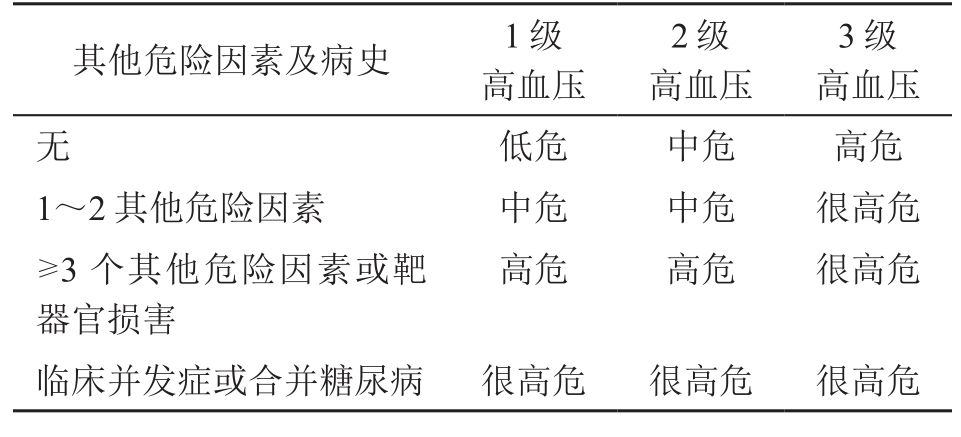
\includegraphics[width=3.1875in,height=1.44792in]{./images/Image00555.jpg}
\end{table}

\subsubsection{高血压的治疗原则与目标}

高血压治疗的基本原则:①高血压是一种以动脉血压持续升高为特征的进行性“心血管综合征”,常伴有其他危险因素、靶器官损害或临床疾患,需要进行综合干预。②抗高血压治疗包括非药物和药物两种方法,大多数患者需长期、甚至终生坚持治疗。③定期测量血压;规范治疗,改善治疗依从性,尽可能实现降压达标;坚持长期平稳有效地控制血压。

治疗高血压的主要目的是最大限度地降低心脑血管并发症发生和死亡的总体危险。因此,应在治疗高血压的同时,干预所有其他的可逆性心血管危险因素(如吸烟、血脂异常或肥胖等),并适当处理同时存在的各种临床情况。危险因素越多,其程度越严重。

高血压患者的降压目标:在患者能耐受的情况下,逐步降压达标。一般高血压患者,应将血压降至140/90mmHg以下;65岁及以上老年人的SBP应控制在150mmHg以下,如能耐受还可进一步降低;伴有肾脏疾病、糖尿病或病情稳定的冠心病的高血压患者治疗更宜个体化,一般可以将血压降至130/80mmHg以下,脑卒中后的高血压患者一般血压目标为<
140/90mmHg。处于急性期的冠心病或脑卒中患者,应按照相关指南进行血压管理。DBP低于60mmHg的冠心病患者,应在密切监测血压的前提下逐渐实现SBP达标。

高血压的治疗策略:按低危、中危、高危及很高危分层,应全面评估患者的总体危险,并在危险分层的基础上作出治疗决策:①高危、很高危患者:一旦确诊,立即开始对高血压及并存的危险因素和临床情况进行综合治疗。②中危患者:先对患者的血压及其他危险因素进行为期数周的观察,反复测量血压,尽可能进行24小时动态血压监测或家庭血压监测评估靶器官损害情况,然后决定是否以及何时开始药物治疗。③低危患者:对患者进行较长时间的观察,反复测量血压,尽可能进行24小时动态血压监测或家庭血压监测,评估靶器官损害情况,然后决定是否以及何时开始药物治疗。

\begin{table}[htbp]
\centering
\caption{影响高血压患者心血管预后的重要因素}
\label{tab150-3}
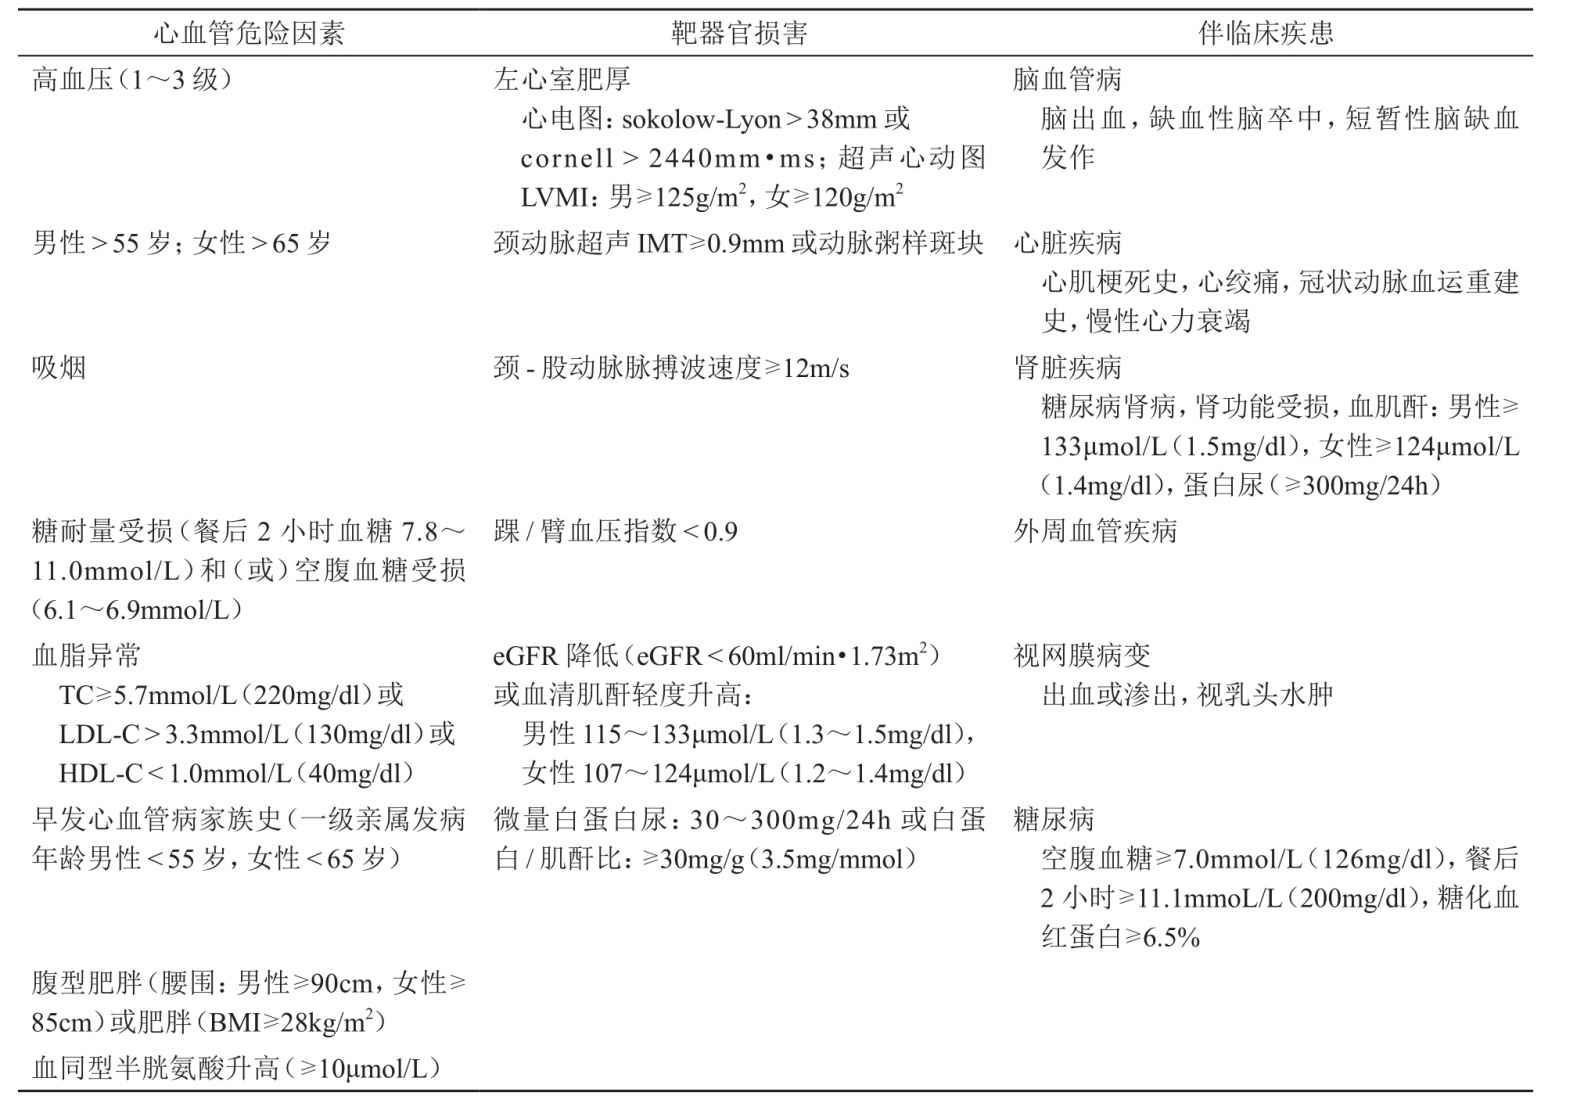
\includegraphics[width=6.73958in,height=4.6875in]{./images/Image00556.jpg}
\end{table}


\subsubsection{高血压的非药物治疗}

高血压的非药物治疗主要指生活方式干预,即去除不利于身体和心理健康的行为和习惯。其不仅可以预防或延迟高血压的发生,还可以降低血压,提高降压药物的疗效,从而降低心血管风险。主要措施包括:①减少钠盐摄入,增加钾盐摄入;②控制体重;③戒烟;④不过量饮酒;⑤体育运动;⑥减轻精神压力,保持心理平衡。

\subsubsection{高血压的药物治疗原则}

高血压的治疗包括药物和非药物治疗。高血压药物治疗应遵循以下4项原则,即小剂量开始,优先选择长效制剂,联合用药及个体化。

\paragraph{小剂量}

初始治疗时通常应采用较小的有效治疗剂量,并根据需要,逐步增加剂量。

\paragraph{优先应用长效制剂}

尽可能使用每天1次给药而有持续24小时降压作用的长效药物,以有效控制夜间血压与晨峰血压,更有效预防心脑血管并发症发生。如使用中、短效制剂,则需每天2~3次给药,以达到平稳控制血压。

\paragraph{联合用药}

可增加降压效果又不增加不良反应,在低剂量单药治疗疗效不满意时,可以采用2种或多种降压药物联合治疗。事实上,2级以上高血压为达到目标血压常需联合治疗。对血压≥160/100mmHg、高于目标血压20/10mmHg或高危及以上患者,起始即可采用小剂量2种药物联合治疗,或用固定配比复方制剂。

\paragraph{个体化}

根据患者具体情况和耐受性及个人意愿或长期承受能力,选择适合患者的降压药物。

当前常用于降压的药物主要有以下五类,即:钙拮抗剂(CCB)、血管紧张素转换酶抑制剂(ACEI)、血管紧张素受体拮抗剂(ARB)、利尿剂(噻嗪类)、β受体阻滞剂。以上五类降压药及固定低剂量复方制剂均可作为高血压初始或维持治疗的选择药物。此外还有α受体阻滞剂、中枢和周围神经交感神经抑制剂、节后交感神经抑制剂及直接血管扩张剂等;还有肾素、内皮素受体拮抗剂、钾通道开放剂等新型降压药。有关钙拮抗剂、血管紧张素转换酶抑制剂、血管紧张素受体拮抗剂、利尿剂(噻嗪类)和β受体阻滞剂等五类降压药的运用见本章第2~8节的阐述;有关降压药的联合应用见本章第9节“抗高血压药物的联合应用”。

\subsubsection{特殊人群高血压的处理原则}

\hypertarget{text00409.htmlux5cux23CHP17-3-1-8-1}{}
(一) 老年高血压

我国 60岁及以上人群高血压的患病率为
49\%。即约每2位60岁以上人中就有1人患高血压。老年高血压常与多种疾病并存,并发症多:常并发冠心病、心力衰竭、脑血管疾病、肾功能不全、糖尿病等。我国人群脑卒中发生率远高于西方人群。若血压长期控制不理想,更易发生靶器官损害。

\paragraph{临床特点}

①SBP增高,脉压增大:老年单纯收缩期高血压占高血压的60\%,随着年龄增长其发生率增加,同时脑卒中的发生率急剧升高。老年人脉压与总死亡率和心血管事件呈显著正相关。②血压波动大:血压“晨峰”现象增多,高血压合并直立性低血压和餐后低血压者增多。直立性低血压定义为:在改变体位为直立位的3分钟内,SBP下降>
20mmHg或DBP下降>
10mmHg,同时伴有低灌注的症状,如头晕或晕厥。老年单纯收缩期高血压伴有糖尿病、低血容量,应用利尿剂、扩血管药或精神类药物者容易发生直立性低血压。老年餐后低血压定义为:餐后2小时内每15分钟测量血压1次,与餐前比较SBP下降>
20mmHg;或餐前SBP≥100mmHg,但餐后<
90mmHg;或虽餐后血压仅有轻微降低,但出现心脑缺血症状(心绞痛、乏力、晕厥、意识障碍)。老年人血压波动大,影响治疗效果,血压急剧波动时,可显著增加发生心血管事件的危险。③常见血压昼夜节律异常:血压昼夜节律异常的发生率高,表现为夜间血压下降幅度<
10\%(非杓型)或超过20\%(超杓型),导致心、脑、肾等靶器官损害的危险增加。④白大衣高血压增多。⑤假性高血压增多,指袖带法所测血压值高于动脉内测压值的现象(SBP升高≥10mmHg或DBP升高≥15mmHg),可见于正常血压或高血压老年人。上述高血压的临床特点与老年动脉硬化性血管壁僵硬度增加及血压调节中枢功能减退有关。

\paragraph{诊断}

年龄≥65岁,血压持续升高或3次以上非同日坐位SBP≥140mmHg和(或)DBP≥90mmHg,可定义为老年高血压。若SBP≥140mmHg,DBP
< 90mmHg,则定义为老年单纯收缩期高血压。

\paragraph{治疗}

老年高血压试验汇总分析表明,降压治疗可使脑卒中减少40\%,心血管事件减少30\%;无论是收缩期或舒张期高血压,抑或是老年单纯收缩期高血压降压治疗均可降低心脑血管病的发生率及死亡率;平均降低SBP
10mmHg和DBP
4mmHg,脑卒中的发生风险降低30\%,心血管事件和死亡率降低13\%,70岁以上的老年男性、脉压增大或存在心血管并发症者获益更多。老年高血压患者的血压应降至150/90mmHg以下,如能耐受可降至140/90mmHg以下。对于80岁以上的高龄老年人的降压的目标值为<
150/90mmHg。老年高血压降压治疗应强调SBP达标,同时应避免过度降低血压;在能耐受降压治疗前提下,逐步降压达标,应避免过快降压;对于降压耐受性良好的患者应积极进行降压治疗。

SBP高而DBP不高甚至低的老年单纯收缩期高血压患者治疗有一定难度。如何处理目前没有明确的证据。建议:当DBP
< 60mmHg,而SBP < 150mmHg,宜观察,可不用药物治疗;如SBP
150~179mmHg,可谨慎给予小剂量降压药治疗;如SBP≥180mmHg,则给予小剂量降压药治疗。降压药可用小剂量利尿剂、CCB、ACEI或ARB等。治疗中应密切观察病情变化。

\hypertarget{text00409.htmlux5cux23CHP17-3-1-8-2}{}
(二) 儿童与青少年高血压

儿童高血压患病率
,学龄前儿童为2\%~4\%,学龄儿童为4\%~9\%。一项20年的队列研究显示,43\%的儿童高血压20年后发展成为成人高血压,而儿童血压正常人群中发展为成人高血压的比例只有9.5\%。左心室肥厚是儿童原发性高血压最突出的靶器官损害,占儿童高血压的10\%~40\%。儿童中血压明显升高者多为继发性高血压,肾性高血压是继发性高血压的首位病因,占继发性高血压的80\%左右。随年龄增长,原发性高血压的比例逐渐升高,进入青春期的青少年高血压多为原发性。50\%以上的儿童高血压伴有肥胖。

\paragraph{诊断}

与成人血压测量不同,儿童与青少年常规测量坐位右上臂肱动脉血压。选择合适袖带对于儿童血压的准确测量非常重要,理想袖带的气囊宽度应至少等于右上臂围的40\%,气囊长度至少包绕上臂围的80\%,气囊宽度与长度的比值至少为1∶2。目前国际上统一采用P90、P95、P99作为诊断“正常高值血压”、“高血压”和“严重高血压”标准。对个体而言,只有经过3次及以上不同时间测量的血压水平≥P95方可诊断为高血压;随后要进行高血压程度的分级:①高血压1级:P95~P99
+ 5mmHg。②高血压2级:≥P99 + 5mmHg。

对儿童与青少年高血压的评估包括以下4个方面:高血压的病因、血压水平的真实性、靶器官损害及程度、其他心血管疾病及并发症。在评估基础上制订合理的治疗计划。

\paragraph{治疗}

原发性高血压或未合并靶器官损害的高血压儿童与青少年应将血压降至P95以下;合并肾脏疾病、糖尿病或出现高血压靶器官损害时,应将血压降至P90以下,以减少对靶器官的损害,降低远期心血管病发病率。绝大多数高血压儿童与青少年通过非药物治疗即可达到血压控制目标。措施:①控制体重,延缓BMI上升。②增加有氧锻炼,减少静态活动时间。③调整饮食结构(包括限盐),建立健康饮食习惯。

高血压儿童与青少年如果合并下述1种及以上情况,则需要开始药物治疗:出现高血压临床症状,继发性高血压,出现高血压靶器官的损害,糖尿病,非药物治疗6个月后无效者。儿童与青少年高血压药物治疗的原则是从单一用药、小剂量开始。ACEI或ARB和CCB在标准剂量下较少发生不良反应,通常作为首选的儿科抗高血压药物;利尿剂通常作为二线抗高血压药物或与其他类型药物联合使用,解决水钠潴留及用于肾脏疾病引起的继发性高血压;其他种类药物如α受体阻滞剂和β受体阻滞剂,因为不良反应的限制多用于严重高血压和联合用药。

\hypertarget{text00409.htmlux5cux23CHP17-3-1-8-3}{}
(三) 妊娠高血压

妊娠合并高血压的患病率占孕妇的
5\%~10\%,其中70\%是与妊娠有关的高血压,其余30\%在妊娠前即存在高血压。妊娠合并高血压分为慢性高血压、妊娠期高血压和先兆子痫3类。慢性高血压指的是妊娠前即证实存在或在妊娠的前20周即出现的高血压。妊娠期高血压为妊娠20周以后发生的高血压,不伴有明显蛋白尿,妊娠结束后血压可以恢复正常。先兆子痫定义为发生在妊娠20周以后的血压升高伴临床蛋白尿(24小时尿蛋白≥300mg);重度先兆子痫定义为血压≥l60/110mmHg,有大量蛋白尿,并出现头痛、视力模糊、肺水肿、少尿和实验室检查异常(如血小板计数下降、转氨酶异常),常合并胎盘功能异常。

\paragraph{降压治疗的策略}

非药物措施(限盐、富钾饮食、适当活动、情绪放松)是妊娠合并高血压安全和有效的治疗方法,应作为药物治疗的基础。由于所有降压药物对胎儿的安全性均缺乏严格的临床验证,而且动物试验中发现一些药物具有致畸作用,因此,药物选择和应用受到限制。妊娠期间的降压用药不宜过于积极,治疗的主要目的是保证母子安全和妊娠的顺利进行。治疗的策略、给药时间的长短及药物的选择取决于血压升高的程度,以及对血压升高所带来危害的评估。在接受非药物治疗措施以后,血压≥150/100mmHg时应开始药物治疗,治疗目标是将血压控制在130~140/80~90mmHg。

\paragraph{妊娠合并高血压的处理}

①轻度妊娠高血压:药物治疗并不能给胎儿带来益处,也没有证据证明可以预防先兆子痫的发生,此时包括限盐在内的非药物治疗是最安全有效的处理方法。对于妊娠前高血压、存在靶器官损害或同时使用多种降压药物的患者,应根据妊娠期间血压水平调整药物剂量,原则上采用尽可能少的药物种类和剂量,同时应充分告知患者,妊娠早期用药对胎儿重要脏器发育影响的不确定性。血压轻度升高的先兆子痫,由于其子痫的发生率仅0.5\%,不建议常规应用硫酸镁,但需要密切观察血压和尿蛋白变化以及胎儿状况。②重度妊娠合并高血压:治疗的主要目的是最大限度降低母亲的患病率和病死率。在严密观察母婴状态的前提下,应明确治疗的持续时间、降压目标、药物选择和终止妊娠的指征。对重度先兆子痫,建议静脉应用硫酸镁,密切观察血压、腱反射和不良反应,并确定终止妊娠的时机。

\paragraph{降压药物的选择}

必要时谨慎使用降压药。常用的静脉降压药物有拉贝洛尔和硫酸镁;口服药物包括β受体阻滞剂、阿米洛利、肼屈嗪或CCB等;硫酸镁是治疗严重先兆子痫的首选药物。妊娠期间禁用ACEI或ARB。

\hypertarget{text00409.htmlux5cux23CHP17-3-1-8-4}{}
(四) 高血压伴脑卒中

\paragraph{病情稳定的脑卒中患者}

血压目标一般应达到<
140mmHg。常用的5种降压药物利尿剂、CCB、ACEI、ARB及β受体阻滞剂均能通过降压而发挥预防脑卒中或短暂性脑缺血作用。利尿剂及某些降压药物可能效果更好些。可选择单药或联合用药。

\paragraph{急性脑卒中的血压处理}

(1) 急性缺血性脑卒中溶栓前血压应控制在< 185/
110mmHg。急性缺血性脑卒中发病24小时内血压升高的患者应谨慎处理,除非SBP≥180mmHg或DBP≥100mmHg或伴有严重心功能不全、主动脉夹层、高血压脑病者,一般不予降压。降压的合理目标是24小时内血压降低约15\%。有高血压病史且正在服用降压药物者,如神经功能平稳,可于脑卒中后24小时开始使用降压药物。

(2) 急性脑出血患者,如果SBP > 200mmHg或平均动脉压>
150mmHg,要考虑用持续静脉滴注给药,积极降低血压,血压的监测频率为每5分钟1次。如果SBP
>180mmHg或平均动脉压>
130mmHg,并有疑似颅内压升高的证据者,要考虑监测颅内压,用间断或持续的静脉给药降低血压;如没有疑似颅内压升高的证据,则考虑用间断或持续的静脉给药轻度降低血压(例如,平均动脉压110mmHg或目标血压为160/90mmHg),密切观察病情变化。

\hypertarget{text00409.htmlux5cux23CHP17-3-1-8-5}{}
(五) 高血压伴冠心病

前瞻性协作研究表明,血压在115/75~180/115mmHg范围内冠心病的危险呈持续上升的趋势,且每增加20/10mmHg,冠心病危险增加一倍。建议稳定性冠心病、不稳定型心绞痛、非ST段抬高和ST段抬高心肌梗死的高血压患者目标血压水平一般可为<
130/80mmHg,但治疗宜个体化。如患者冠状动脉严重病变或年龄大于65岁,DBP尽量维持在60mmHg以上。对于老年高血压且伴脉压大的患者,降压治疗可导致DBP过低(<
60mmHg)。

\hypertarget{text00409.htmlux5cux23CHP17-3-1-8-6}{}
(六) 高血压合并心力衰竭

降压治疗可降低高血压患者心力衰竭的发生率,也可减少伴心力衰竭患者的心血管事件,降低病死率和改善预后。对于既往曾患心力衰竭或目前仍有心力衰竭症状与体征的高血压患者,应积极控制高血压。降压的目标水平为<
130/80mmHg。对于持续高血压患者,或高血压伴左心室肥厚,或伴左心室功能障碍但无心衰症状和体征的患者,治疗目标亦为<
130/80mmHg。这样做有利于预防出现心衰的症状和体征。

药物选择和应用:对于伴心力衰竭或LVEF降低的患者,临床研究表明,阻断RAAS药物如ACEI或ARB、醛固酮受体阻滞剂(螺内酯、依普利酮)。以及交感神经系统阻滞剂及β受体阻滞剂等均对患者的长期预后有益。高血压伴心力衰竭患者通常需合用2种或3种降压药物。在应用利尿剂消除体内过多滞留的液体,使患者处于“干重”状态后,β受体阻滞剂加ACEI或ARB可发挥协同的有益作用,称之为优化组合。此种组合既为抗心力衰竭治疗所必需,又可发挥良好的降压作用。RAAS阻滞剂和β受体阻滞剂均应从小剂量起始,约为通常降压治疗剂量的1/8~1/4,且应缓慢地增加剂量,直至达到抗心力衰竭治疗所需要的目标剂量或最大耐受剂量。

\hypertarget{text00409.htmlux5cux23CHP17-3-1-8-7}{}
(七) 高血压伴肾脏疾病

\paragraph{高血压与肾脏疾病}

两者存在伴发关系,高血压病可引起肾脏损害,后者又使血压进一步升高,并难以控制。肾脏疾病所致的高血压称之为肾性高血压,主要由肾血管疾病(如肾动脉狭窄)和肾实质性疾病(肾小球肾炎,慢性肾盂肾炎、多囊肾等)所致,在肾脏疾病进展过程中可产生高血压,后者又加剧肾脏病变使肾功能减退,形成恶性循环。

\paragraph{高血压所致肾脏损害的降压治疗}

高血压患者如出现肾功能损害的早期表现,如微量白蛋白尿或肌酐水平轻度升高,应积极控制血压,在患者能够耐受情况下,可将血压降至<
130/80mmHg,必要时可联合应用2~3种降压药物,其中应包括一种RAAS阻滞剂(ACEI或ARB)。

\paragraph{高血压伴慢性肾脏病的降压治疗}

此类患者,尤其伴肾功能不全,饮食及血压控制最为重要。严格控制血压,是延缓肾脏病变的进展,预防心血管事件发生风险的关键。目标血压可控制在130/80mmHg以下。ACEI或ARB既有降压,又有降低蛋白尿的作用,因此,对于高血压伴肾脏病患者,尤其有蛋白尿患者,应作为首选;而这两类药物联合对于减少蛋白尿可能有益,但尚缺乏足够循证依据。如不能达标可加用长效CCB和利尿剂。若肾功能显著受损如血肌酐>
3mg/dl,或肾小球滤过率低于30ml/(min•1.73m\textsuperscript{2}
)或有大量蛋白尿,此时宜首先用二氢吡啶类CCB;噻嗪类利尿剂可改用袢利尿剂(如呋塞米)。

\paragraph{终末期肾病的降压治疗}

未透析者一般不用ACEI或ARB及噻嗪类利尿剂;可用CCB、袢利尿剂等降压治疗。对肾脏透析患者,应密切监测血钾和肌酐水平,降压目标<
140/90mmHg。

\hypertarget{text00409.htmlux5cux23CHP17-3-1-8-8}{}
(八) 高血压合并糖尿病

高血压常合并糖代谢异常。高血压人群的糖尿病患病率平均为18\%。高血压也是糖尿病心血管和微血管并发症患者的重要危险因素。糖尿病一旦合并高血压,可使患者心脑血管事件的风险显著增加(至少是单纯高血压或单纯糖尿病的2倍),并加速视网膜病变以及肾脏病变的发生和发展,其死亡风险将增加7.2倍。

\paragraph{降压治疗的目标}

一般糖尿病患者的降压目标是<
130/80mmHg;老年或伴严重冠心病的糖尿病患者血压目标是< 140/90mmHg。

\paragraph{药物的选择和应用}

SBP在130~139mmHg或者DBP在80~89mmHg的糖尿病患者,可以进行不超过3个月的非药物治疗,包括饮食管理、减重、限制钠盐摄入、适当限酒和中等强度的规律运动。如血压不能达标,应采用药物治疗。血压≥140/90mmHg的患者,应在非药物治疗的基础上立即开始药物治疗;伴微量白蛋白尿的患者,应该直接使用药物治疗。首先考虑使用ACEI或ARB,对肾脏有保护作用,且有改善糖、脂代谢的益处;当需要联合用药时,应以ACEI或ARB为基础。亦可应用利尿剂、β受体阻滞剂或二氢吡啶类CCB。利尿剂和β受体阻滞剂宜小剂量使用,糖尿病合并高尿酸血症的患者,慎用利尿剂;反复低血糖发作者,慎用β受体阻滞剂,以免掩盖低血糖症状。有前列腺肥大且血压控制不佳的患者可使用α受体阻滞剂。血压达标通常需要2种或2种以上的药物联合治疗。

\hypertarget{text00409.htmlux5cux23CHP17-3-1-8-9}{}
(九) 代谢综合征

我国代谢综合征患病率随着年龄增加而升高
,至65岁达高峰,50岁之前男性高于女性,而50岁之后则相反。我国成人代谢综合征诊断标准:腰围,男性≥90cm,女性≥85cm;血压≥130/85mmHg,或有高血压病史;甘油三酯≥1.70mmol/L;高密度脂蛋白胆固醇<
1.04mmol/L;空腹血糖≥6.1mmol/L,糖负荷2小时血糖≥7.8mmol/L,或有糖尿病史。满足上述3项者即可作出诊断。我国代谢综合征的主要类型以肥胖合并高血压和血脂异常最为常见,占53.7\%,其次为肥胖合并糖代谢异常和高血压,占30.5\%。

治疗原则和降压目标:代谢综合征的治疗重在早期干预,健康膳食和合理运动甚为重要。其干预要求主要组分综合达标:可考虑血压<
130/80mmHg,如合并肾脏损害,血压控制要求更严;空腹血糖水平<
6.1mmol/L;甘油三酯< 1.7mmol/L;高密度脂蛋白胆固醇> 1.04mmol/L;腰围<
90cm(男)或< 85cm(女)。降压药物主要推荐ACEI
或ARB,也可应用二氢吡啶类CCB和保钾利尿剂,慎用β受体阻滞剂和噻嗪类利尿剂。

\subsubsection{难治性高血压}

在改善生活方式的基础上,应用了足量且合理联合的3种降压药物(包括利尿剂)后,血压仍在目标水平之上,或至少需要4种药物才能使血压达标时,称为难治性高血压(或顽固性高血压),约占高血压患者的15\%~20\%。

\paragraph{难治性高血压原因的筛查}

①判断是否为假性难治性高血压:常见为测压方法不当(如测量时姿势不正确、上臂较粗者未使用较大的袖带);单纯性诊室(白大衣)高血压。结合家庭自测血压、动态血压监测可使血压测定结果更接近真实。②寻找影响高血压的病因和并存的疾病因素:包括与药物应用有关的原因,如患者顺从性差(未坚持服药)、降压药物选择使用不当(剂量偏低、联合用药不够合理),以及仍在应用拮抗降压的药物(如口服避孕药,肾上腺类固醇类、可卡因、甘草、麻黄等);未改变不良生活方式或改变失败(体重增加或肥胖、吸烟、重度饮酒);容量负荷过重(利尿剂治疗不充分、高盐摄入、进展性肾功能不全);以及伴慢性疼痛和长期焦虑等。患者可能存在1种以上可纠正或难以纠正的原因。③排除上述因素后,应启动继发性高血压的筛查。

\paragraph{处理原则}

①此类患者最好转高血压专科治疗。②多与患者沟通,提高长期用药的依从性,并严格限制钠盐摄入。③选用适当的联合方案:先采用3种药的方案例如:ACEI或ARB
+ CCB
+噻嗪类利尿剂,或由扩血管药、减慢心率药和利尿剂组成的3药联合方案,能够针对血压升高的多种机制,体现平衡的高效降压的特点,往往可以奏效。效果仍不理想者可再加用一种降压药如螺内酯、β受体阻滞剂、α受体阻滞剂或交感神经抑制剂(可乐定)。④调整联合用药方案:在上述努力失败后,可在严密观察下停用现有降压药,重启另一种治疗方案。

\subsubsection{高血压急症和亚急症}

高血压急症和高血压亚急症曾被称为高血压危象。高血压急症是指原发性或继发性高血压患者,在某些诱因作用下,血压突然和显著升高(一般超过180/120mmHg),同时伴有进行性心、脑、肾等重要靶器官功能不全的表现。高血压急症包括高血压脑病、颅内出血(脑出血和蛛网膜下腔出血)、脑梗死、急性心力衰竭、肺水肿、急性冠状动脉综合征(不稳定型心绞痛、急性非ST段抬高和ST段抬高心肌梗死)、主动脉夹层、子痫等,应注意血压水平的高低与急性靶器官损害的程度并非呈正比。一部分高血压急症并不伴有特别高的血压值,如并发于妊娠期或某些急性肾小球肾炎的患者,但如血压不及时控制在合理范围内会对脏器功能产生严重影响,甚至危及生命,处理过程中需要高度重视。并发急性肺水肿、主动脉夹层、心肌梗死者,即使血压仅为中度升高,也应视为高血压急症。

高血压亚急症是指血压显著升高但不伴靶器官损害。患者可以有血压明显升高造成的症状,如头痛,胸闷,鼻出血和烦躁不安等。相当多的患者有服药顺从性不好或治疗不足的问题。

血压升高的程度不是区别高血压急症与高血压亚急症的标准,区别两者的唯一标准是有无新近发生的急性进行性的严重靶器官损害。

高血压急症和亚急症的诊断与处理,详见本书第42章“高血压危象”部分。

\subsubsection{围术期高血压}

围术期高血压是指外科手术住院期间(包括手术前、手术中和手术后,一般3~4天)伴发的急性血压增高(SBP、DBP或平均动脉压超过基线20\%以上)。手术后高血压常开始于术后10~20分钟,可能持续4小时。如果不及时治疗,患者易发生出血、脑卒中和心肌梗死。在围术期的过程中出现短时间血压增高,并超过180/110mmHg时称为围术期高血压危象,其发生率为4\%~35\%。既往有高血压病史,特别是DBP超过110mmHg者易发生围术期血压波动。易发生高血压的手术类型有:颈动脉、腹部主动脉、外周血管、腹腔和胸腔手术。严重高血压易发生在以下手术过程中:心脏、大血管(颈动脉内膜剥脱术、主动脉手术)、神经系统和头颈部的手术、此外还有肾脏移植以及大的创伤等(烧伤或头部创伤)。

\paragraph{降压治疗的目标}

治疗目的是保护靶器官功能。降压目标取决于手术前患者血压情况,一般应降至基线的10\%;易出血或严重心力衰竭患者可以将血压降至更低。需严密监测患者对治疗的反应并及时调整降压药物剂量。轻中度原发性高血压且不伴代谢紊乱或心血管系统异常时,不需延期手术。3级高血压(≥180/110mmHg)应权衡延期手术的利弊再做决定。如在围术期出现高血压急症,通常需要静脉给予降压药物,即刻目标是在30~60分钟内使DBP降至110mmHg左右,或降低10\%~15\%,但不超过25\%。如果患者可以耐受,应在随后的2~6小时将血压降低至160/100mmHg。主动脉夹层患者降压速度应更快,在24~48小时内将血压逐渐降至基线水平。应选用那些起效迅速,作用时间短的药物如拉贝洛尔、艾司洛尔、尼卡地平、硝酸甘油、硝普钠和非诺多泮。

\paragraph{围术期高血压的防治}

高血压患者在手术前应继续降压治疗,术前数日宜换用长效降压药物并在手术当天早晨继续服药。有证据表明,术前β受体阻滞剂的应用可以有效减少血压波动、心肌缺血以及术后房颤发生,还可降低非心脏手术的死亡率。反之,停用β受体阻滞剂和可乐定可以引起血压和心率的反跳。不能口服的患者可以使用静脉或舌下含服的β受体阻滞剂,也可以使用可乐定皮肤贴剂。术中血压骤升应积极寻找并及时处理各种可能的原因,如疼痛、血容量过多、低氧血症、高碳酸血症和体温过低等。

\protect\hypertarget{text00410.html}{}{}

\section{钙拮抗剂}

钙拮抗剂(calcium channel
blocker,CCB),又称钙通道阻滞剂,降压作用主要通过选择性地阻滞Ca\textsuperscript{2+}
经细胞膜上的L型钙通道进入血管平滑肌细胞内,减少细胞内Ca\textsuperscript{2+}
浓度的药物,从而减弱Ca\textsuperscript{2+}
所介导的兴奋-收缩偶联,降低阻力血管的收缩反应性。钙通道阻滞剂还能减轻血管紧张素Ⅱ和α\textsubscript{1}
肾上腺素能受体的缩血管效应,减少肾小管钠重吸收。根据其作用于L型钙通道的α\textsubscript{1}
亚单位的不同结合位点,又分为2类:二氢吡啶类,以硝苯地平、氨氯地平为代表;非二氢吡啶类,可细分为硫氮{}
酮类、苯烷胺类,分别以地尔硫{}
、维拉帕米为代表。根据作用药物作用时间长短又将CCB类分为短效和长效。长效制剂,起效变得较慢,血药浓度波动小,血压控制相对平稳,且不改变血压变化的昼夜规律;可避免短效制剂所致的反射性交感神经兴奋,不良反应的发生率明显降低;作用时间长,用药次数少,长期用药的安全性好,使患者的依从性得到加强,这是长效钙通道阻滞剂的突出优点。目前主张使用长效钙通道阻滞剂降压。

常用CCB类药物主要制剂及用量见表\ref{tab150-4}。

\begin{table}[htbp]
\centering
\caption{常用的钙拮抗剂}
\label{tab150-4}
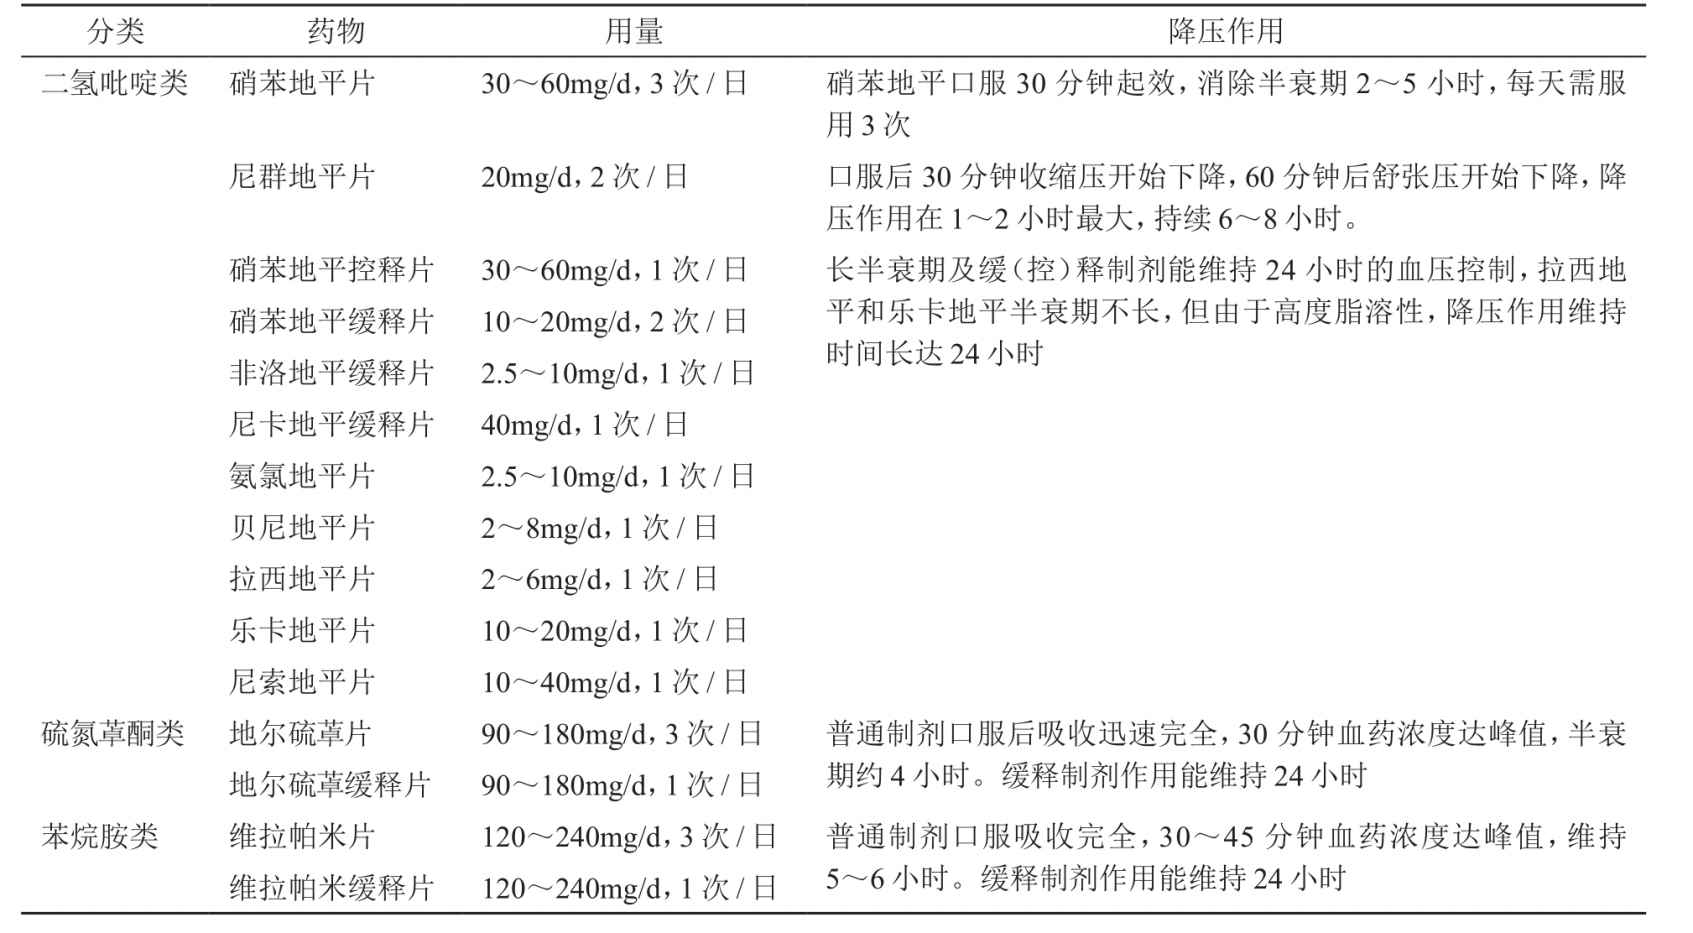
\includegraphics[width=6.71875in,height=3.69792in]{./images/Image00559.jpg}
\end{table}

\paragraph{临床用药要点}

钙离子拮抗剂可用于不同程度的高血压。可单药或与其他4类药联合应用。降压治疗最好选用长效钙拮抗剂,应避免使用短效钙拮抗剂。其中二氢吡啶类钙拮抗剂在我国抗高血压临床试验证据较多,均证实可减少脑卒中事件发生。二氢吡啶类钙拮抗剂适用于以下类型高血压:①老年人高血压;②单纯收缩期高血压;③合并周围血管疾病;④合并稳定型心绞痛;⑤合并糖耐量减低;⑥合并肾脏损害;⑦合并颈动脉粥样硬化;⑧合并冠状动脉粥样硬化。非二氢吡啶类该拮抗剂适用于以下类型高血压:①合并心绞痛;②合并颈动脉粥样硬化;③合并室上性心动过速。可单药或与其他4类药联合应用。

\paragraph{禁忌证}

妊娠、窦房结功能低下、传导阻滞、心衰、严重主动脉狭窄者禁用硫氮{}
酮和苯烷胺类钙拮抗剂。不稳定型心绞痛、急性心肌梗死者禁用短效二氢吡啶类拮抗剂,伴有心力衰竭或心动过速者慎用二氢吡啶类类钙拮抗剂。维拉帕米不宜与β受体阻断剂合用。

\paragraph{副作用}

①二氢吡啶类:头痛、颜面潮红及心悸(心跳反射性加快)、踝部水肿、牙龈增生。②非二氢吡啶类:头痛和颜面潮红,但较二氢吡啶类少见;便秘;房室传导阻滞、心脏停搏、负性肌力作用。

\protect\hypertarget{text00411.html}{}{}

\section{血管紧张素转化酶抑制剂}

血管紧张素转换酶抑制剂(angiotensin converting enzyme
inhibitors,ACEI)竞争性地抑制血管紧张素转换酶,阻断血管紧张素Ⅰ(AngⅠ)转换成血管紧张素Ⅱ(AngⅡ),从而减低了循环中以及局部组织中的AngⅡ水平,抑制AngⅡ所介导的血管收缩作用。ACEI还减少醛固酮和加压素的释放、降低交感神经活性、减弱AngⅡ的多种作用。此外,ACEI通过抑制激肽酶而增高缓激肽水平,后者刺激B\textsubscript{2}
受体,促进扩血管因子一氧化氮(NO)和有血管活性作用的前列腺素(前列环素和前列腺素E\textsubscript{2}
)的生成。ACEI还能阻断血管紧张素1-7的降解,使其水平增加,从而通过加强刺激血管紧张素1-7受体,进一步起到扩张血管及抗增生作用。众多临床研究表明,ACEI可显著降低心血管病患者的病死率、致残率。ACEI已成为治疗心血管病的基石。ACEI可根据其与ACE分子表面锌原子相结合的活性基团而分成巯基类、羧基类和膦酸基类等三类。

常用ACEI主要制剂及用量见表\ref{tab150-5}。

\paragraph{临床用药要点}

血管紧张素转换酶抑制剂类药物可用于治疗不同程度高血压,尤其适用于轻中度高血压的治疗,对老年性高血压也有效,特别适用于肾性血管性高血压。血管紧张素转换酶抑制剂适用于以下类型高血压:①合并左心室肥厚;②合并左心功能不全;③合并心肌梗死;④合并非糖尿病肾病;⑤合并糖尿病、糖尿病肾病;⑥合并颈动脉粥样硬化;⑦合并蛋白尿或微量白蛋白尿。血管紧张素转换酶抑制剂类药物已被推荐为以下情况的首选降压药物:高血压合并糖尿病或有糖尿病家族史、糖尿病肾病、糖耐量轻微受损;高脂血症;心衰;痛风或有痛风家族史;周围血管疾病;高肾素性高血压;收缩期高血压;动脉顺应性差;左室肥厚、心肌梗死后防止左室重构;为维持正常代谢状态及为改善患者生活质量(认知功能、性功能、运动耐力);低钠摄入或低肾素性高血压伴低钠饮食。ACEI一般从小剂量开始逐渐递增,直至靶剂量(临床试验中证实能提高生存率的剂量),并维持使用。可与利尿剂、钙拮抗剂联用。

\begin{table}[htbp]
\centering
\caption{常用的 ACEI}
\label{tab150-5}
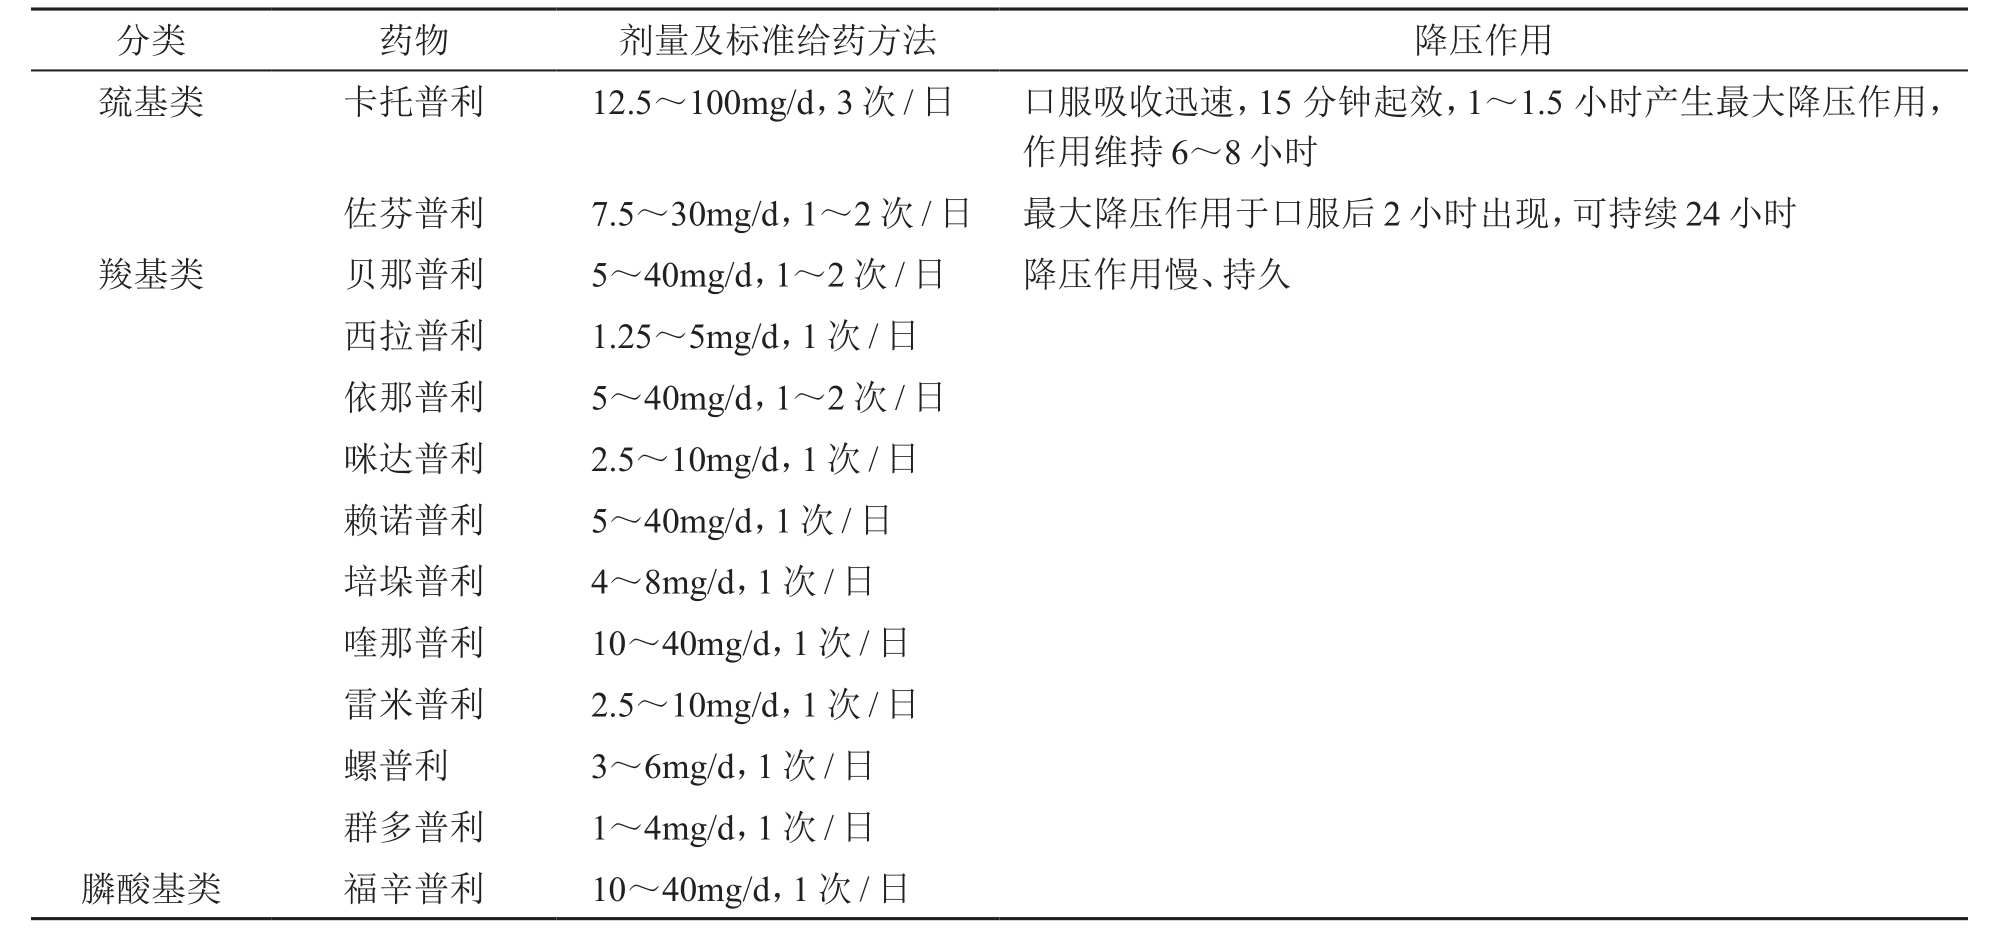
\includegraphics[width=6.70833in,height=3.14583in]{./images/Image00561.jpg}
\end{table}

\paragraph{禁忌证}

血管神经性水肿、ACEI过敏、双侧肾动脉狭窄或单侧肾动脉狭窄伴另一侧肾切除、妊娠、高血钾、肾功能不全(血肌酐>
265μmol/L)、左室流出道梗阻(主动脉瓣狭窄及梗阻型肥厚性心肌病)。

\paragraph{副作用}

①干咳:最常见,发生率约5\%~10\%,停药7~10天后可消失;②低血压:常见,多数无症状;③高钾血症:较常见于慢性心力衰竭、老年、肾功能受损、糖尿病、补充钾盐或合用保钾利尿剂、肝素或非甾体类抗炎药物的患者;④肾功能损害:ACEI用药最初2个月可增加血尿素氮或肌酐水平,升幅<
30\%为预期反应,可继续治疗;肌酐上升过高(升幅>
30\%~50\%)为异常反应,提示肾缺血,应停药,寻找缺血病因并设法排除,待肌酐正常后再用。肾功能异常患者使用ACEI,以选择经肝肾双通道排泄的ACEI为好;⑤胎儿畸形;⑥其他:血管神经性水肿、味觉减退、粒细胞减少、皮疹,均较少见。

\protect\hypertarget{text00412.html}{}{}

\section{血管紧张素Ⅱ受体拮抗剂}

血管紧张素Ⅱ受体拮抗剂(angiotensinⅡ receptor
blocker,ARB)对AngⅡ的1型受体(AT\textsubscript{1}
)有高亲和力,通过选择性阻断AngⅡ经AT\textsubscript{1}
受体介导的各种效应降压。同时ARB使血浆肾素活性及AngⅡ水平升高,对AngⅡ的2型受体(AT\textsubscript{2}
)的激动作用加强,也可能产生有利影响,如扩张血管、降低血压、抗组织增生作用等。

常用ARB主要制剂及用量见表\ref{tab150-6}。

\paragraph{临床用药要点}

与ACEI相同。且可用于不能耐受ACEI引起干咳患者的降压。可与钙拮抗剂、利尿剂联用。

\paragraph{禁忌证}

与ACEI相同。

\paragraph{副作用}

目前尚未发现有明显的不良反应,可有轻度头晕、恶心等,偶可致高钾血症。血管神经性水肿罕见。

\begin{table}[htbp]
\centering
\caption{常用的 ARB}
\label{tab150-6}
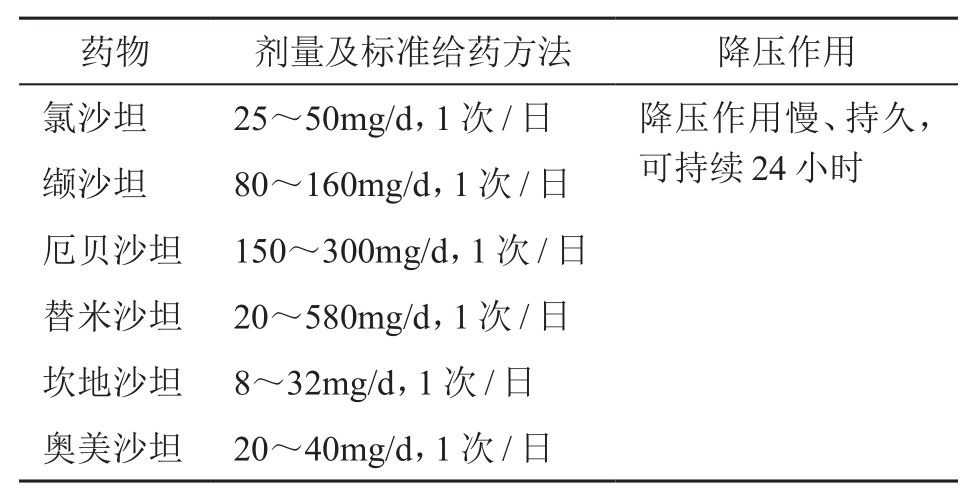
\includegraphics[width=3.25in,height=1.65625in]{./images/Image00562.jpg}
\end{table}

\protect\hypertarget{text00413.html}{}{}

\section{利尿剂}

利尿剂的降压机制有两种:一种是通过利尿来促进人体排钠,从而减少患者的血容量,使其心输出量降低,从而达到降压的目的;二是通过利尿来促进人体排钠,使患者血管平滑肌钠离子的含量降低,减弱小动脉平滑肌对加压物质的反应,从而使患者的血管扩张,达到降压的目的。根据其在肾脏作用的部位可分为:①噻嗪类利尿剂,主要作用于远曲小管近端;②袢利尿剂,主要作用于髓袢升支粗段髓质部和皮质部;③保钾利尿剂:主要作用于近曲小管和集合管。

常用利尿剂主要制剂及用量见表\ref{tab150-7}。

\paragraph{临床用药要点}

小剂量噻嗪类利尿剂适用于:①轻中度高血压;②老年单纯收缩期高血压;③肥胖、盐摄入过多的高血压;④合并充血性心力衰竭的高血压;⑤老年高血压;⑥老老年高血压。袢利尿剂适用于:高血压并充血性心力衰竭、肾功能不全以及高血压急症时的迅速降压。保钾利尿剂适用于:高血压并充血性心力衰竭;其中醛固酮拮抗剂(螺内酯、依普利酮)可用于醛固酮增多症。临床最常用的为氢氯噻嗪和吲达帕胺,降压时主张小剂量使用。可与钙拮抗剂、ACEI、ARB联用。

\begin{table}[htbp]
\centering
\caption{常用的利尿剂}
\label{tab150-7}
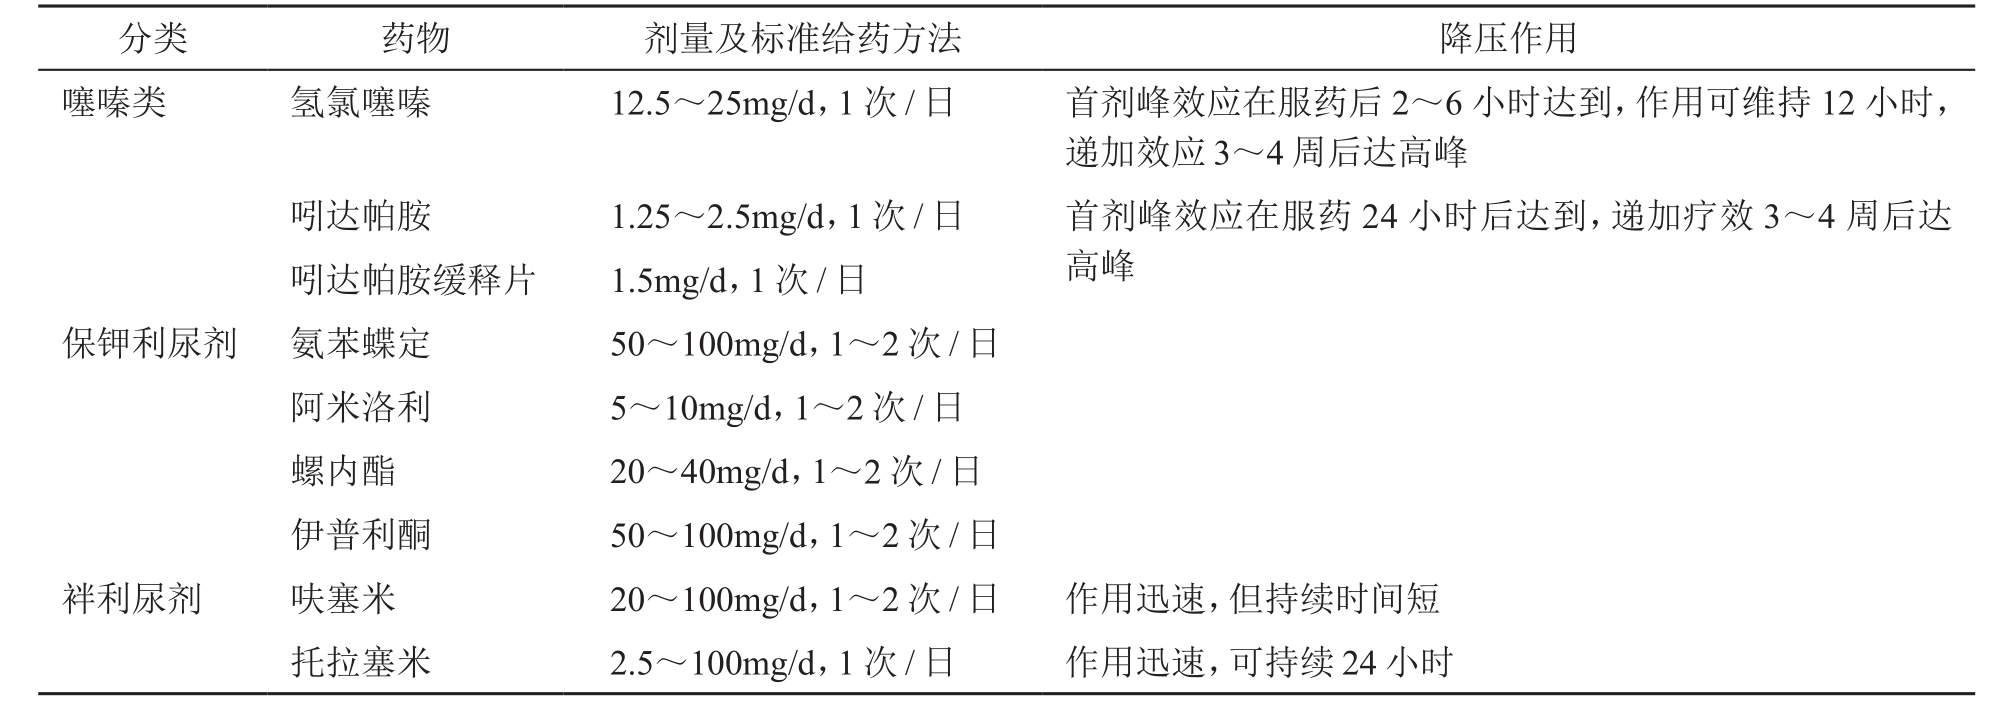
\includegraphics[width=6.65625in,height=2.375in]{./images/Image00563.jpg}
\end{table}

\paragraph{禁忌证}

噻嗪类禁忌:低血钾、高钙血症、糖尿病、高脂血症、用药前低血容量、肾功能不全(血肌酐>
265μmol/L)、严重肝功能损害、高尿酸血症或痛风、磺胺类药物过敏。保钾利尿剂禁用于高钾血症、痛风。

\paragraph{副作用}

噻嗪类利尿剂副作用与剂量有关,小剂量可使副作用明显减低,常见副作用有:血容量不足、低血钠、低血钾、血糖代谢异常、高尿酸、低镁等。保钾利尿剂副作用:高血钾、胃肠道症状、小腿痉挛、月经紊乱、阳痿、醛固酮拮抗剂可导致男性乳房发育等。呋塞米副作用与噻嗪类相似。

\protect\hypertarget{text00414.html}{}{}

\section{β受体阻滞剂}

β受体阻滞剂主要通过以下机制降压:①阻滞中枢β受体,使兴奋性神经元活动降低而外周交感神经张力降低;②拮抗血管平滑肌突触前膜肾上腺素能β受体,阻止其促使外周交感神经末梢去甲肾上腺素及肾上腺素释放的正反馈效应;③阻滞肾小球旁器的肾上腺素β\textsubscript{1}
受体,使肾素分泌减少,使血管紧张素水平下降;④抑制心脏β\textsubscript{1}
受体而致心率减慢,心搏出量减少。β受体阻滞剂可分为选择性(作用于β\textsubscript{1}
受体)、非选择性(作用于β\textsubscript{1} 、β\textsubscript{2}
受体)、兼有α受体阻滞作用三类。

常用β受体阻滞剂及用量见表\ref{tab150-8}。

\paragraph{临床用药要点}

适用于:①各种不同程度的高血压;②合并劳力性心绞痛或心肌梗死后的高血压;③合并有心动过速的高血压;④合并有稳定型心力衰竭的高血压;⑤合并有焦虑症的高血压。可与钙拮抗剂联用。

\paragraph{禁忌证}

主要有:支气管痉挛性肺病、严重心动过缓、二度以上房室传导阻滞、病态窦房结综合征、急性心力衰竭、妊娠早期和晚期、血脂异常、糖尿病、周围血管病、运动员。

\paragraph{副作用}

主要不良反应有:心动过缓、房室传导阻滞、负性肌力作用、支气管痉挛。其他不良反应有:疲乏、性功能障碍、影响血糖血脂代谢。长时间较高剂量使用后突然停药可引起撤药综合征。

\protect\hypertarget{text00415.html}{}{}

\section{α受体阻滞剂}

α受体阻滞剂降压机制是通过选择性地阻断血管平滑肌的α受体,使周围血管阻力下降。可分为选择性α受体阻滞剂(选择性作用于α\textsubscript{1}
受体)、非选择性α受体阻滞剂(作用于α\textsubscript{1}
受体、α\textsubscript{2} 受体)。

常用α受体阻滞剂及用量见表\ref{tab150-9}。

\paragraph{临床用药要点}

选择性α受体阻滞剂可用于各种程度的高血压,更适用于高血压伴血脂异常、血糖异常、前列腺肥大患者。非选择性α受体阻滞剂适用于嗜铬细胞瘤引起的高血压。

\paragraph{禁忌证}

不用于直立性低血压患者,慎用于老年患者、心功能不全。

\paragraph{副作用}

直立性低血压、头昏、乏力、心动过速等。

\begin{table}[htbp]
\centering
\caption{常用的β受体阻滞剂}
\label{tab150-8}
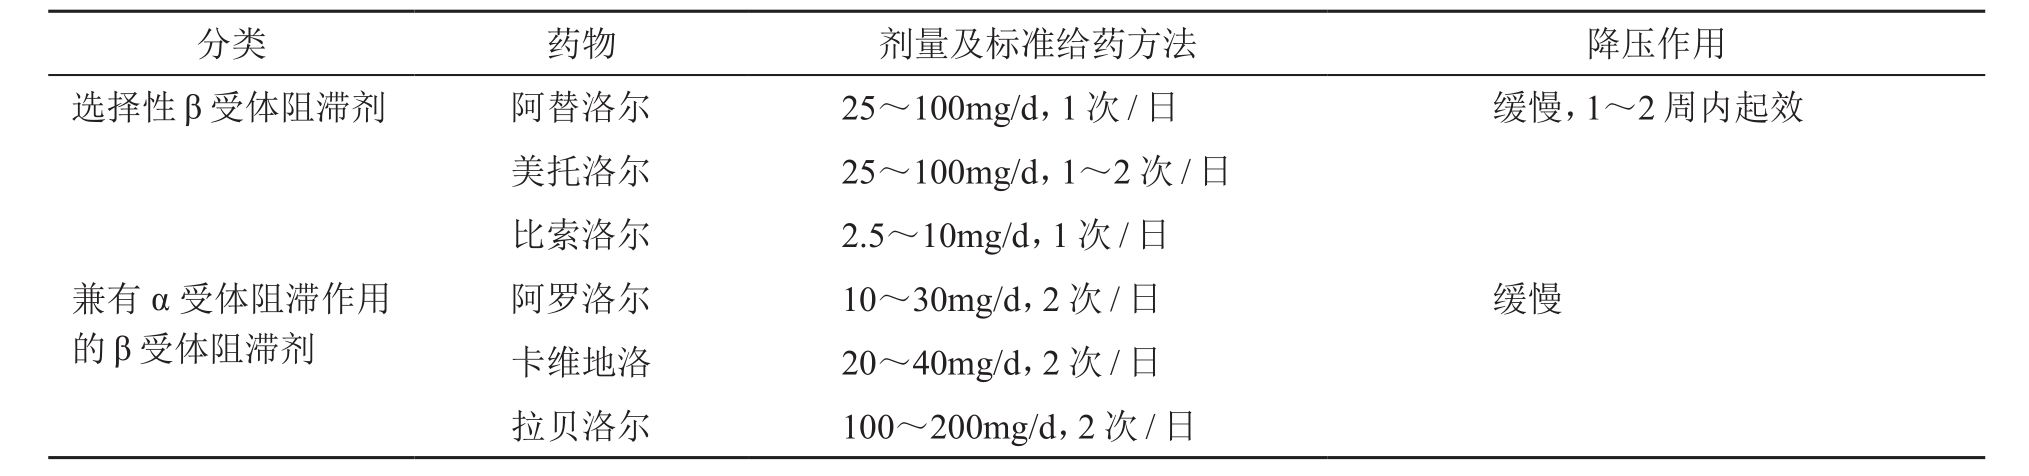
\includegraphics[width=6.75in,height=1.58333in]{./images/Image00564.jpg}
\end{table}

\begin{table}[htbp]
\centering
\caption{常用α受体阻滞剂}
\label{tab150-9}
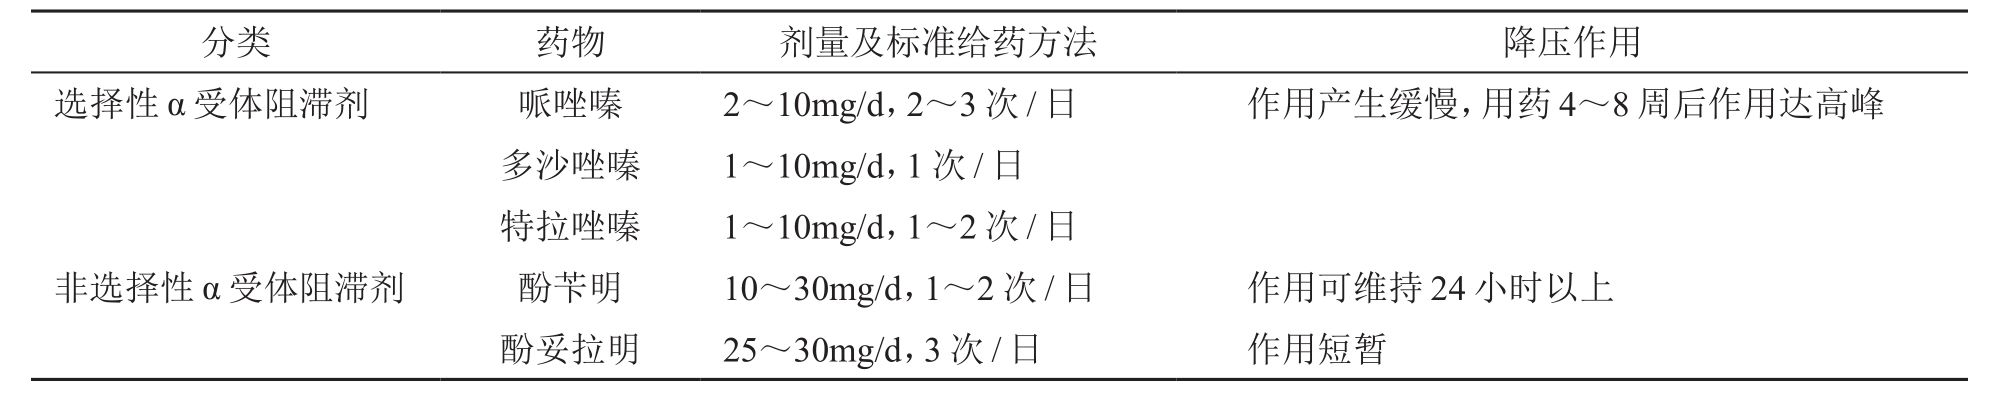
\includegraphics[width=6.65625in,height=1.33333in]{./images/Image00565.jpg}
\end{table}

\protect\hypertarget{text00416.html}{}{}

\section{直接血管扩张剂}

直接血管扩张剂直接作用于小动脉平滑肌使动脉扩张而降压。

常用的为静脉应用的硝普钠。静脉滴注后起效迅速(1~2分钟),失效亦快(停药后1~3分钟),在5~15分钟内血压即恢复至用药前水平。常规用法为:50mg硝普钠加入5\%葡萄糖液50ml中以5~10μg/min速率泵入,每5~10分钟调整一次,每次增加5~10μg/min,直至达到目标血压。

\paragraph{临床用药要点}

硝普钠适用于高血压急症的紧急降压。用药不宜超过72小时。药物易见光分解,应用时需临时配置,每6~8小时更换一次药物,药物需避光输注。停药时应逐渐减量,并加用口服血管扩张剂,以免出现症状“反跳”。

\paragraph{禁忌证}

维生素B\textsubscript{12}
缺乏者及儿童忌用;肝肾功能不全、甲状腺功能减退者、孕妇及老人慎用。

\paragraph{副作用}

用药过程中可出现恶心、呕吐、精神不安、肌肉痉挛、头痛、厌食、皮疹、出汗、发热等;长期或大剂量使用,尤其对肾功能衰竭患者,可能引起硫氰化物蓄积而导致甲状腺功能减退及氰化物中毒,亦可出现险峻的低血压症。

\protect\hypertarget{text00417.html}{}{}

\section{抗高血压药物的联合应用}

联合应用降压药物已成为降压治疗的基本方法。为了达到目标血压水平,许多高血压患者需要应用≥2种降压药物。

\paragraph{联合用药的适应证}

2级高血压、高于目标血压20/10mmHg和(或)伴有多种危险因素、靶器官损害或临床疾患的高危人群,往往初始治疗即需要应用2种小剂量降压药物,如仍不能达到目标血压,可在原药基础上加量或可能需要3种,甚至4种以上降压药物。

\paragraph{联合用药的方法}

两药联合时,降压作用机制应具有互补性,同时具有相加的降压作用,并可互相抵消或减轻不良反应。例如,在应用ACEI或ARB基础上加用小剂量噻嗪类利尿剂,降压效果可以达到甚至超过将原有的ACEI
或ARB剂量倍增的降压幅度。同样加用二氢吡啶类CCB也有相似效果。

\paragraph{联合用药方案}

①ACEI或ARB
+噻嗪类利尿剂:ACEI和ARB可使血钾水平略有上升,能拮抗噻嗪类利尿剂长期应用所致的低血钾等不良反应。ACEI或ARB
+噻嗪类利尿剂合用有协同作用,有利于改善降压效果。②二氢吡啶类CCB +
ACEI或ARB:CCB具有直接扩张动脉的作用,ACEI或ARB既扩张动脉、又扩张静脉,故两药合用有协同降压作用。二氢吡啶类CCB常见的不良反应为踝部水肿,可被ACEI或ARB抵消。CHIEF研究表明,小剂量长效二氢吡啶类CCB
+
ARB初始治疗高血压患者,可明显提高血压控制率。此外,ACEI或ARB也可部分阻断CCB所致反射性交感神经张力增加和心率加快的不良反应。③CCB
+噻嗪类利尿剂:FEVER研究证实,二氢吡啶类CCB
+噻嗪类利尿剂治疗,可降低高血压患者脑卒中发生的风险。④二氢吡啶类CCB +
β受体阻滞剂:CCB具有的扩张血管和轻度增加心率的作用,恰好抵消β受体阻滞剂的缩血管及减慢心率的作用。两药联合可使不良反应减轻。

我国临床主要推荐应用优化联合的治疗方案是:二氢吡啶类CCB +
ARB;二氢吡啶类CCB + ACEI;ARB +噻嗪类利尿剂;ACEI
+噻嗪类利尿剂;二氢吡啶类CCB +噻嗪类利尿剂;二氢吡啶类CCB +
β受体阻滞剂。

次要推荐使用的联合治疗方案是:利尿剂+β受体阻滞剂;α受体阻滞剂+
β受体阻滞剂;二氢吡啶类CCB +保钾利尿剂;噻嗪类利尿剂+保钾利尿剂。

不常规推荐的但必要时可慎用的联合治疗方案是:ACEI + B受体阻滞剂;ARB +
β受体阻滞剂;ACEI + ARB;中枢作用药+β受体阻滞剂。

多种药物的合用:①三药联合的方案:在上述各种两药联合方式中加上另一种降压药物便构成三药联合方案,其中二氢吡啶类CCB
+
ACEI(或ARB)+噻嗪类利尿剂组成的联合方案最为常用。②4种药联合的方案:主要适用于难治性高血压患者,可以在上述三药联合基础上加用第4种药物如β受体阻滞剂、螺内酯、可乐定或α受体阻滞剂等。

\paragraph{固定配比复方制剂}

是常用的一组高血压联合治疗药物。通常由不同作用机制的两种降压药组成,也称为单片固定复方制剂。与随机组方的降压联合治疗相比,其优点是使用方便,可改善治疗的依从性及疗效,是联合治疗的新趋势。对2或3级高血压或某些高危患者可作为初始治疗的选择药物之一。应用时注意其相应组成成分的禁忌证或可能的不良反应。

我国传统的固定配比复方制剂:包括复方利血平(复方降压片)、复方利血平氨苯蝶啶片(降压0号)、珍菊降压片等。以当时常用的利血平、氢氯噻嗪、盐酸双屈嗪或可乐定为主要成分,此类复方制剂组成的合理性虽有争议,但仍在基层广泛使用。

新型的固定配比复方制剂:一般由不同作用机制的两种药物组成,多数每天口服1次,使用方便,改善依从性。目前我国上市的新型的固定配比复方制剂主要包括:ACEI
+噻嗪类利尿剂,ARB +噻嗪类利尿剂;二氢吡啶类CCB + ARB,二氢吡啶类CCB
+β受体阻滞剂,噻嗪类利尿剂+保钾利尿剂等。

降压药与其他心血管治疗药物组成的固定配比复方制剂:有二氢吡啶类CCB
+他汀、ACEI
+叶酸;此类复方制剂使用应基于患者合并的危险因素或临床疾患。需掌握降压药和相应非降压药治疗的适应证及禁忌证。

\protect\hypertarget{text00418.html}{}{}

\hypertarget{text00418.htmlux5cux23CHP17-3-10}{}
参 考 文 献

中国高血压防治指南修订委员会.中国高血压防治指南2010.中华心血管病杂志,2011,39(7):579-615

\protect\hypertarget{text00419.html}{}{}

\chapter{抗心律失常药}

在正常情况下,心脏的冲动来自窦房结,依次经心房、房室结、房室束及普氏纤维,最后传至心室肌,引起心脏节律性收缩。在病理状态时或在药物的影响下,冲动形成失常,或传导发生障碍或二者兼有,就产生心律失常。根据心律失常发作时心室率的快慢可分为快速性心律失常和过缓性心律失常两大类。本章着重介绍抗快速性心律失常药物。

\section{抗心律失常药的基本电生理作用}

此类药物的基本电生理作用是影响心肌细胞膜的离子通道,改变离子流而改变细胞的电生理特性。针对心律失常发生的机制,可将药物的基本电生理作用概括为以下几项:

\paragraph{降低自律性}

药物抑制快反应细胞4相Na\textsuperscript{+}
内流或抑制慢反应细胞4相Ca\textsuperscript{2+}
内流就能降低自律性。药物通过促进K\textsuperscript{+}
外流而增大最大舒张电位,使其远离阈电位降低自律性。

\paragraph{减少后除极与触发活动}

后除极(after depolarization)是在一个动作电位(action
potential,AP)中继0相除极后所发生的除极,其频率较快,振幅较小,呈振荡性波动,膜电位不稳定,容易引起异常冲动的发放,这称为触发活动(trigged
activity)。后除极分早后除极与迟后除极两种,前者发生在完全复极之前的2或3相中,主要由Ca\textsuperscript{2+}
内流增多所引起;后者发生在完全复极之后的4相中,是细胞内Ca\textsuperscript{2+}
过多诱发Na\textsuperscript{+}
短暂内流所引起。因此,钙拮抗剂和钠通道抑制药对减少后除极和触发活动有效。

\paragraph{改变膜反应性而改变传导性}

膜反应性是指膜电位水平与其所激发的0相上升最大速率之间的关系,一般膜电位高,0相上升速率快,振幅大,传导速度也快;反之,则传导减慢。增强膜反应性改善传导或减弱膜反应性而减慢传导都能取消折返激动,前者因改善传导而取消单向阻滞,因此停止折返激动,某些促K\textsuperscript{+}
外流加大最大舒张电位的药如苯妥英钠有此作用;后者因减慢传导而使单向传导阻滞发展成双向阻滞,从而停止折返激动,某些抑制Na\textsuperscript{+}
内流的药如奎尼丁有此作用。

\paragraph{改变}

ERP及APD而减少折返
心肌细胞的静息膜电位,膜内负于膜外约−90mV,处于极化状态。心肌细胞受刺激而兴奋时,发生除极和复极,形成动作电位,它分为5个时相,0相为除极期,是Na\textsuperscript{+}
经快通道迅速进入细胞所致;1相为快速复极初期,由K\textsuperscript{+}
短暂外流所致;2相为缓慢复极期,由Ca\textsuperscript{2+}
及少量Na\textsuperscript{+}
经慢通道进入细胞所致;3相为快速复极末期,由K\textsuperscript{+}
外流所致。0相至3相的时程合称为动作电位时间(action potential
duration,APD)。在复极过程中,当膜电位恢复到−50~−60mV时,细胞才对刺激发生可扩布的动作电位,从除极开始到这以前的一段时间即为有效不应期(effective
refractory
period,ERP),它反映快通道恢复有效开放所需的最短时间,其时间长短一般与APD的长短变化相应,但程度可有不同,一个APD中,ERP比值大,就意味着心肌不起反应的时间延长,不易发生快速性心律失常。药物对ERP和APD约有以下三种可能的影响:

\hypertarget{text00419.htmlux5cux23CHP17-4-1-4-1}{}
(1) 延长APD和ERP:

但延长ERP更为显著,奎尼丁类药物能抑制Na\textsuperscript{+}
通道,使其恢复重新开放的时间延长,即延长ERP,这称绝对延长ERP。ERP/APD之比值较正常为大,即说明在一个APD中ERP占时增多,冲动将有更多机会落入ERP中,折返易被取消。

\hypertarget{text00419.htmlux5cux23CHP17-4-1-4-2}{}
(2) 缩短APD和ERP:

但缩短APD更显著,利多卡因类药物有此作用。因缩短APD更明显,故ERP/APD比值仍较正常大,这称相对延长ERP,同样能取消折返。

\hypertarget{text00419.htmlux5cux23CHP17-4-1-4-3}{}
(3) 促使邻近细胞ERP的不均一(长短不一)趋向均一:

也可防止折返的发生。一般延长ERP的药物,使ERP较长的细胞延长较少,ERP较短者延长较多,从而使长短不一的ERP较为接近。反之亦然,缩短ERP的药物,使ERP短者,缩短少些;ERP长者,缩短多些。故在不同条件下,这些药物都能发挥促使ERP均一的效应。

根据药物的作用机制及针对心律失常的心电生理改变和发生机制,选用药物的基本原则可参考表\ref{tab151-1}。

\begin{longtable}{c}
 \caption{抗心律失常药选用的基本原则}
 \label{tab151-1}
 \endfirsthead
 \caption[]{抗心律失常药选用的基本原则}
 \endhead
 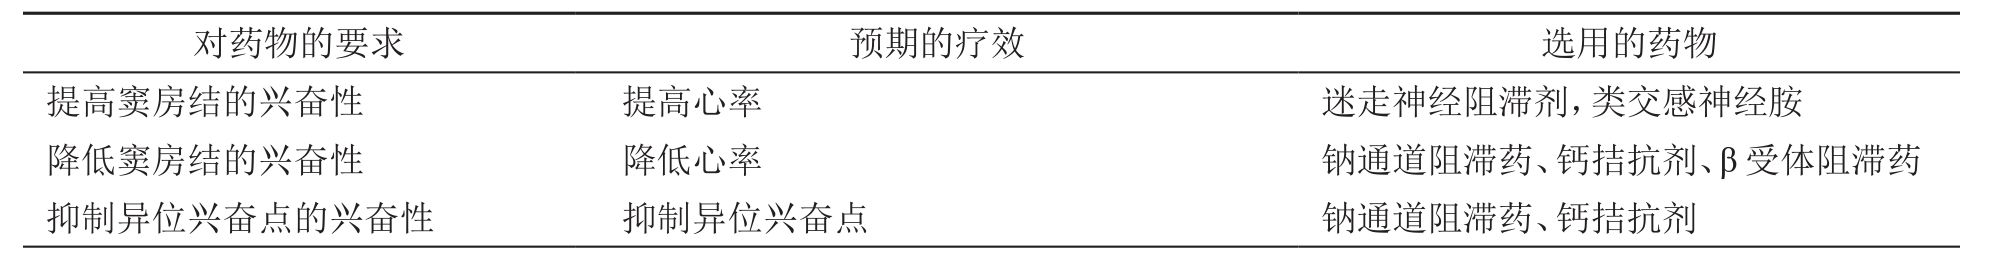
\includegraphics[width=\textwidth,height=\textheight,keepaspectratio]{./images/Image00566.jpg}\\
 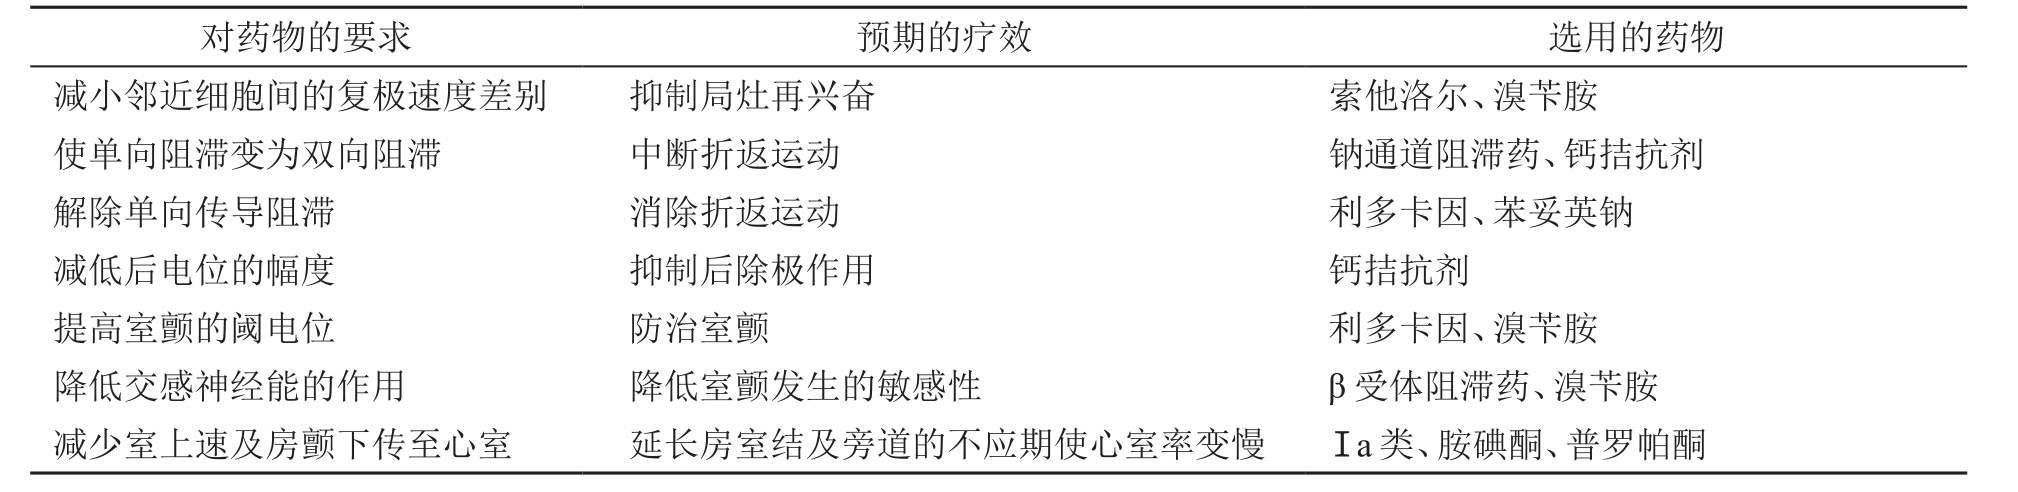
\includegraphics[width=\textwidth,height=\textheight,keepaspectratio]{./images/Image00567.jpg}
 \end{longtable}

\protect\hypertarget{text00420.html}{}{}

\section{抗快速性心律失常药的分类}

现今临床上常用的抗心律失常药虽不过二十几种,但已有几种分类方法。因各分类方法都存在缺陷,至今尚无一个较完善的分类方法。下面简要介绍Williams分类法和Sicilian
Gambit(西西里分类法)。

Williams分类法于1971年首先由Vaugham
Williams提出,后经Harrison等修改,将抗心律失常药分为以下四大类:

\subsubsection{Ⅰ类------钠通道阻滞药}

Ⅰ类以钠通道阻滞为主。根据药物与通道作用动力学和阻滞强度的不同,又分为三个亚类:Ⅰa类:抑制钠通道开放,降低动作电位0相上升速率(Vmax),同时抑制钾外流,延长动作电位时间,以奎尼丁(quinidine)为代表,还包括普鲁卡因胺(procainamide)、丙吡胺(disopyramide)等;Ⅰb类:抑制钠通道,促进钾外流,不影响复极,以利多卡因(lidocaine)为代表,还包括美西律(mexiletine)、苯妥英钠(phenytoin)、室安卡因(tocainide)等;Ⅰc类:在这三个亚类中,Ⅰc类药物对钠通道的阻滞作用是最强的,使快反应细胞Vmax下降,传导下降,有效不应期延长,自律性下降,而对复极过程影响较小。以普罗帕酮(心律平,propafenone)为代表,还包括氟卡尼(flecainide)、恩卡尼(encainide)等。见表\ref{tab151-2}。

Ⅰ类药物与钠通道的结合/解离动力学有很大差别,结合/解离时间常数<
1秒者为Ⅰb类药物;≥12秒者为Ⅰc类药物;介于二者之间者为Ⅰa类药物。Ⅰ类药物与开放和失活状态的通道亲和力大,因此呈使用依赖。对病态心肌、严重心功能障碍和缺血心肌特别敏感,应用要谨慎,尤其Ⅰc类药物,易诱发致命性心律失常。

\subsubsection{Ⅱ类------β受体阻滞药}

阻滞β\textsubscript{2}
肾上腺素能受体,降低交感神经效应,减轻由β\textsubscript{2}
受体介导的心律失常。此类药能降低I\textsubscript{Ca-L}
、起搏电流(I\textsubscript{f)}
,由此减慢窦律,抑制自律性,也能减慢房室结的传导。对病态窦房结综合征或房室传导障碍者作用特别明显。长期口服对病态心肌细胞的复极时间可能有所缩短,能降低缺血心肌的复极离散度,并能提高致颤阈值,由此降低冠心病的猝死率。此类药物有普萘洛尔、阿替洛尔、噻吗洛尔、美多洛尔等。

\subsubsection{Ⅲ类------动作电位延长剂}

为延长动作电位(APD)和有效不应期药(ERP)药,对钾、钠、钙通道均有一定阻滞作用,但以对钾通道的阻滞为主。对APD的延长以对2相平台期的延长为主(Ⅰ\textsubscript{k}
阻滞),对3相影响较小,且本类药物可使原来APD较短的组织获得更多的延长,使心肌细胞间不应期的差异缩小,与奎尼丁呈明显对比。对钙、钠通道的阻滞使自律性降低。对房室结和旁道传导都有作用。

根据对钾通道及其他通道、受体作用的选择性和特点,Ⅲ类药又可分为以下几种:

\hypertarget{text00420.htmlux5cux23CHP17-4-2-3-1}{}
(1) 单纯型I\textsubscript{kr} 阻滞剂:

快速延迟整流钾流(I\textsubscript{kr}
)是心动过缓时的主要复极电流,阻断I\textsubscript{kr}
可使APD和ERP延长,故此类药物在心率减慢时作用最大,表现为逆使用依赖(reverse
use
dependence),易诱发尖端扭转性室速。以d-索他洛尔、阿莫兰特(almokalant)、多非利特(dofetilide)、伊布利特(ibutilide)为代表。SWORD(survial
with oral d-sotalol trial)试验的结果提示单纯性阻滞I\textsubscript{kr}
的Ⅲ类药物并不是最好的选择。

\hypertarget{text00420.htmlux5cux23CHP17-4-2-3-2}{}
(2) 单纯型I\textsubscript{ks} 阻滞剂:

\begin{table}[htbp]
\centering
\caption{Ⅰ类抗心律失常药物的分类}
\label{tab151-2}
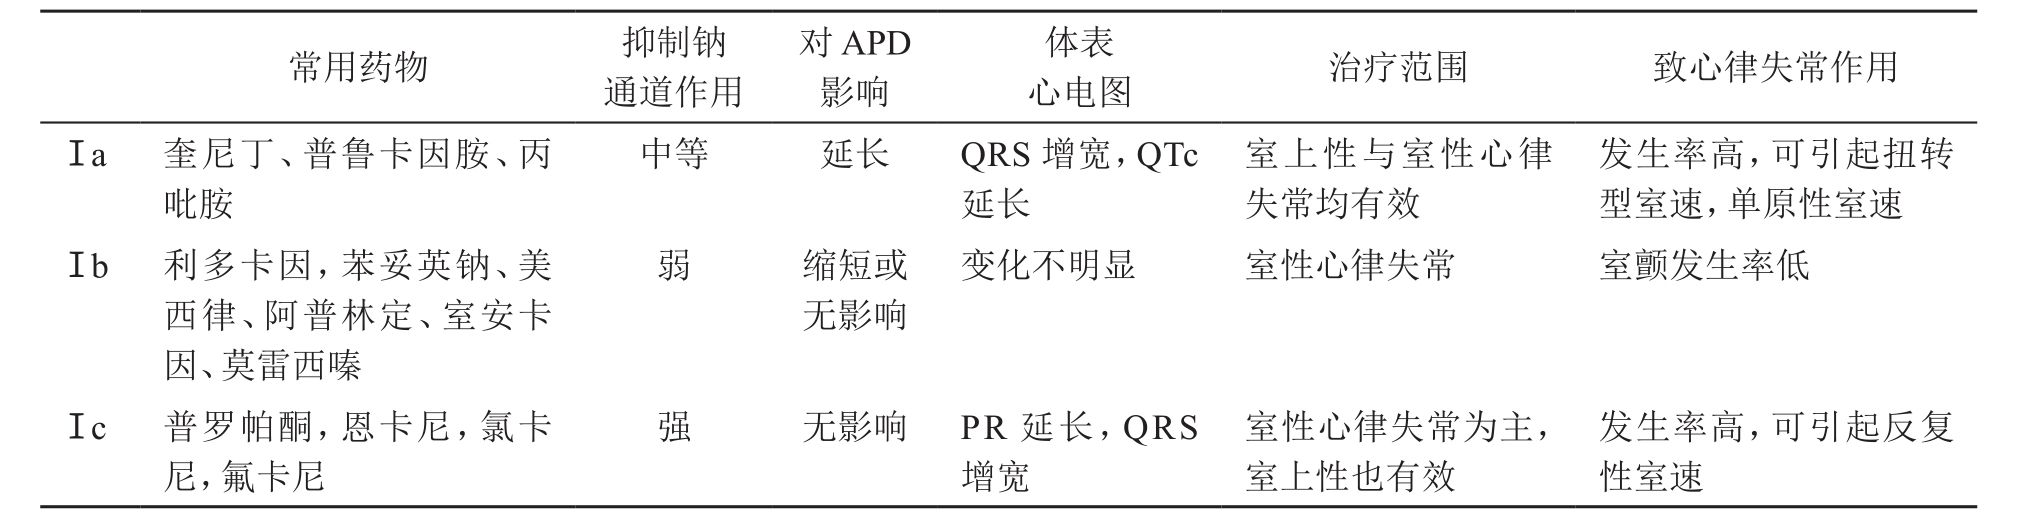
\includegraphics[width=6.78125in,height=1.75in]{./images/Image00568.jpg}
\end{table}

此类药物被认为具有正使用频率依赖性,即心率增加时,对APD和ERP延长较明显,而在心率减慢时对APD和ERP的延长减弱,致心律失常作用弱于I\textsubscript{kr}
阻滞剂,这也是该类药物的最大优点,其代表化合物有Chromanol
293B、HMR21556等。

\hypertarget{text00420.htmlux5cux23CHP17-4-2-3-3}{}
(3) 复合型Ⅲ类抗心律失常药:

形成严重心律失常是由于多离子通道(离子流)异常,使除极/复极过程失去平衡,尤其是复极化延长和(或)不均一所致,所以抗心律失常药应能双向调节心肌APD。在治疗严重心律失常的药效学方面,复合型Ⅲ类抗心律失常药明显优于单纯型。由于复合型Ⅲ类抗心律失常药物不仅阻滞I\textsubscript{kr}
,亦可阻滞I\textsubscript{Na} 、I\textsubscript{Ca}
及α、β受体等,这种复合阻滞机制更加适于纠正离子通道病变。

根据其对其他离子通道、受体阻滞作用的不同,复合型Ⅲ类抗心律失常药又可分为4大类:①无钙通道阻滞作用类,如替地沙米(tedisamil);②有阻滞钙通道作用类,如胺碘酮、阿齐利特(azimilide)等;③有β受体阻滞作用类,如d-索他洛尔、胺碘酮等;④有α受体阻滞作用类,如胺碘酮等。

决奈达隆(dronedarone)是胺碘酮的类似物,与胺碘酮相比,因其不含碘故无心脏外毒性,且半衰期为1~2天,更便于调整药物剂量。ADONIS试验揭示决奈达隆可以使房颤复发率降低25\%,全因死亡或再住院率减少27\%,观察组再住院率为22.8\%,安慰剂组为30.9\%。ERATO试验提示,该药在静息和症状限制性运动中,均能有效控制心室率,没有尖端扭转性室速和心脏外毒性的发生。

\subsubsection{Ⅳ类------钙通道阻滞药}

主要阻滞心肌细胞I\textsubscript{Ca-L} 。I\textsubscript{Ca-L}
介导兴奋收缩偶联,减慢窦房结、房室结的传导,并降低自律性,对早后除极和晚后除极电位及I\textsubscript{Ca-L}
参与的心律失常有治疗作用。此类药物常用的有维拉帕米、地尔硫{}
,可延长房室结有效不应期,有效地终止房室结折返性心动过速,减慢房颤的心室率,也能终止维拉帕米敏感的室速。负性肌力作用较强。

其他尚有腺苷、阿托品及洋地黄等。Williams分类法因其简单易于掌握而被广泛采用。

西西里策略(Sicilian
Gambit):由于心肌细胞的电活动机制是相当复杂的,一种具体的抗心律失常药,可能作用于多种通道、受体,通道阻滞而起到抗心律失常作用,而通道、受体的激活也可起到抗心律失常作用,或促心律失常作用;因此并不像Williams分类中的那样简单,有些新出现的抗心律失常药不能归于Williams分类中的任何一类。正是认识到Williams分类的不足,由此产生了Sicilian
Gambit分类法,其分类的特点是不再把抗心律失常药分成几类,它仅列出了药物治疗的“靶点”,如胺碘酮对钠、钾、钙通道及α、β受体均有阻滞作用,只不过是对钾通道的阻滞作用最强罢了。Sicilian分类中还包括了通道激动剂及α、β、M\textsubscript{2}
受体的阻滞剂或激动剂,包括了离子泵作用的药物,等。Sicilian分类要求医师在治疗心律失常时,必须先弄清产生心律失常的机制和部位(解剖或功能的),找出其易纠正参数(vulnerable
factor)即“治疗靶点”,因此临床医师必须有丰富的电生理学和药理学知识。但在临床实践中,许多心律失常很难确定其发病机制,亦很难找出易纠正参数,故其理论性强,但不实用,它的最终完善更有待于临床电生理诊断学的发展。

有人提出在这两种分类方法的基础上,加以改良的分类方案,较为实用,不是本节的重点,故不赘述。

\protect\hypertarget{text00421.html}{}{}

\section{常用的抗心律失常药}

临床常用的抗心律失常药物的适应证、不良反应,常用剂量和药代动力学特性分别见表\ref{tab151-3}\footnote{*1987年,心律失常抑制试验(cardiac arrhythmia suppression trial,CAST),选用恩卡尼、氟卡尼和莫雷西嗪,治疗心肌梗死后有左室射血分数减低,无症状或有轻微症状的室性期前收缩患者。研究结果显示恩卡尼、氟卡尼治疗组死亡率显著高于对照组;莫雷西嗪增加早期死亡率,对长期死亡率无影响}和表\ref{tab151-4}。

\begin{longtable}{c}
 \caption{常用抗心律失常药物的适应证与不良反应}
 \label{tab151-3}
 \endfirsthead
 \caption[]{常用抗心律失常药物的适应证与不良反应}
 \endhead
 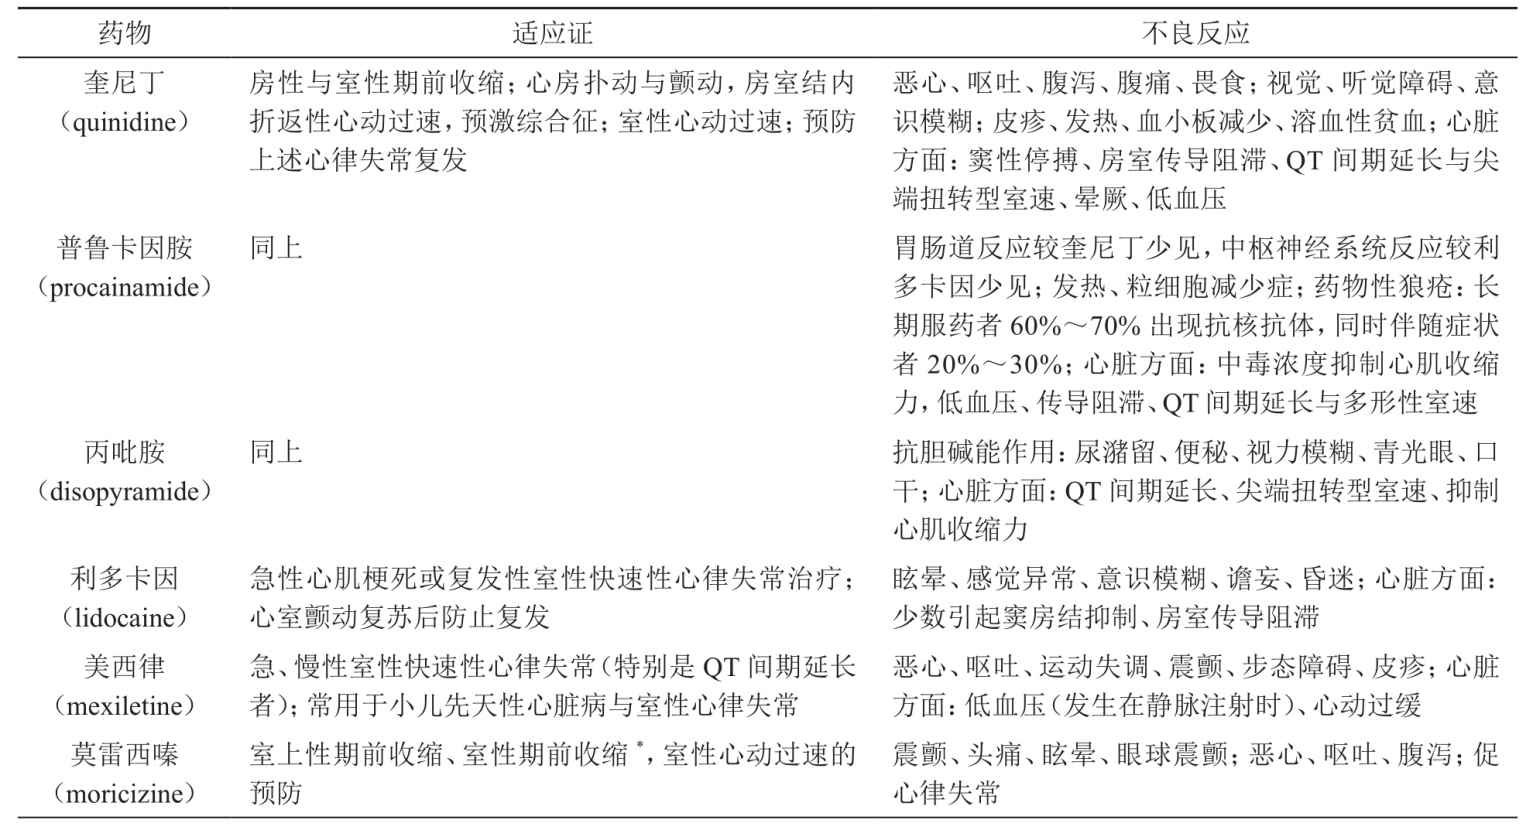
\includegraphics[width=\textwidth,height=\textheight,keepaspectratio]{./images/Image00570.jpg}\\
 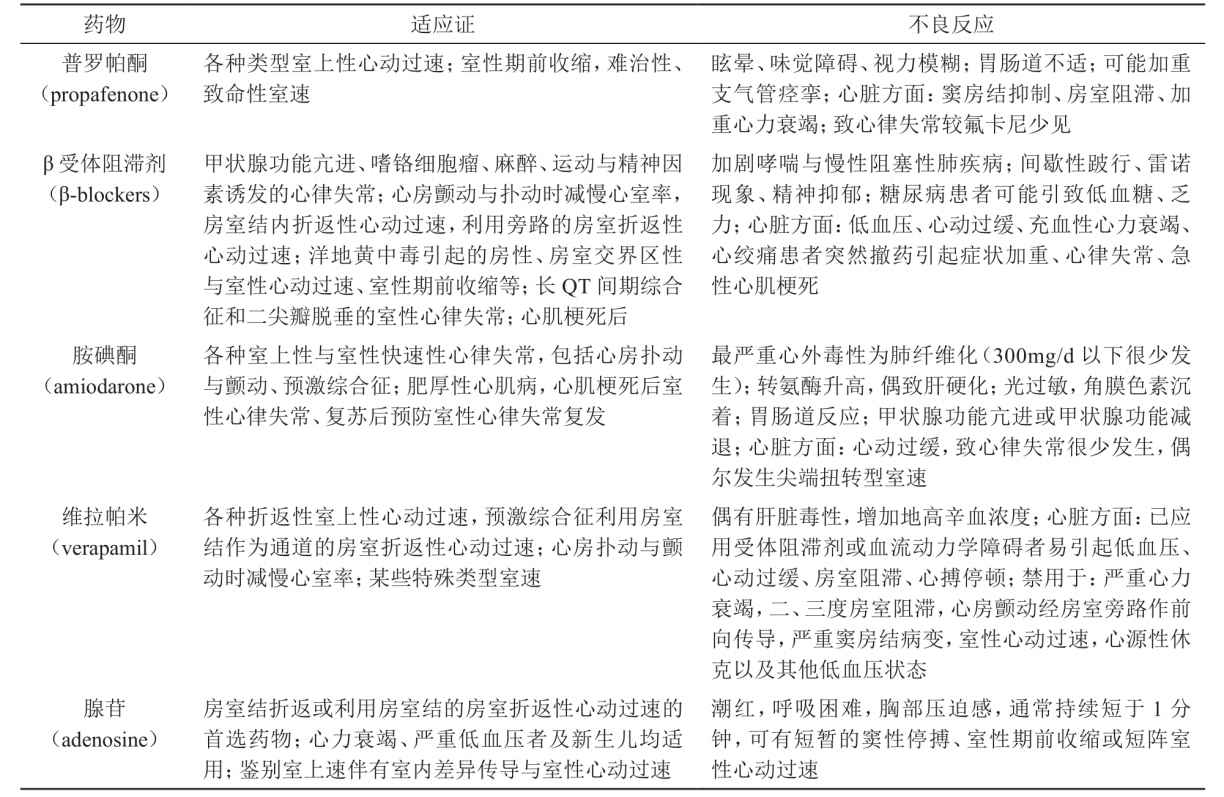
\includegraphics[width=\textwidth,height=\textheight,keepaspectratio]{./images/Image00571.jpg}
 \end{longtable}


\begin{longtable}{c}
 \caption{抗心律失常药物常用剂量与药代动力学特性}
 \label{tab151-4}
 \endfirsthead
 \caption[]{抗心律失常药物常用剂量与药代动力学特性}
 \endhead
 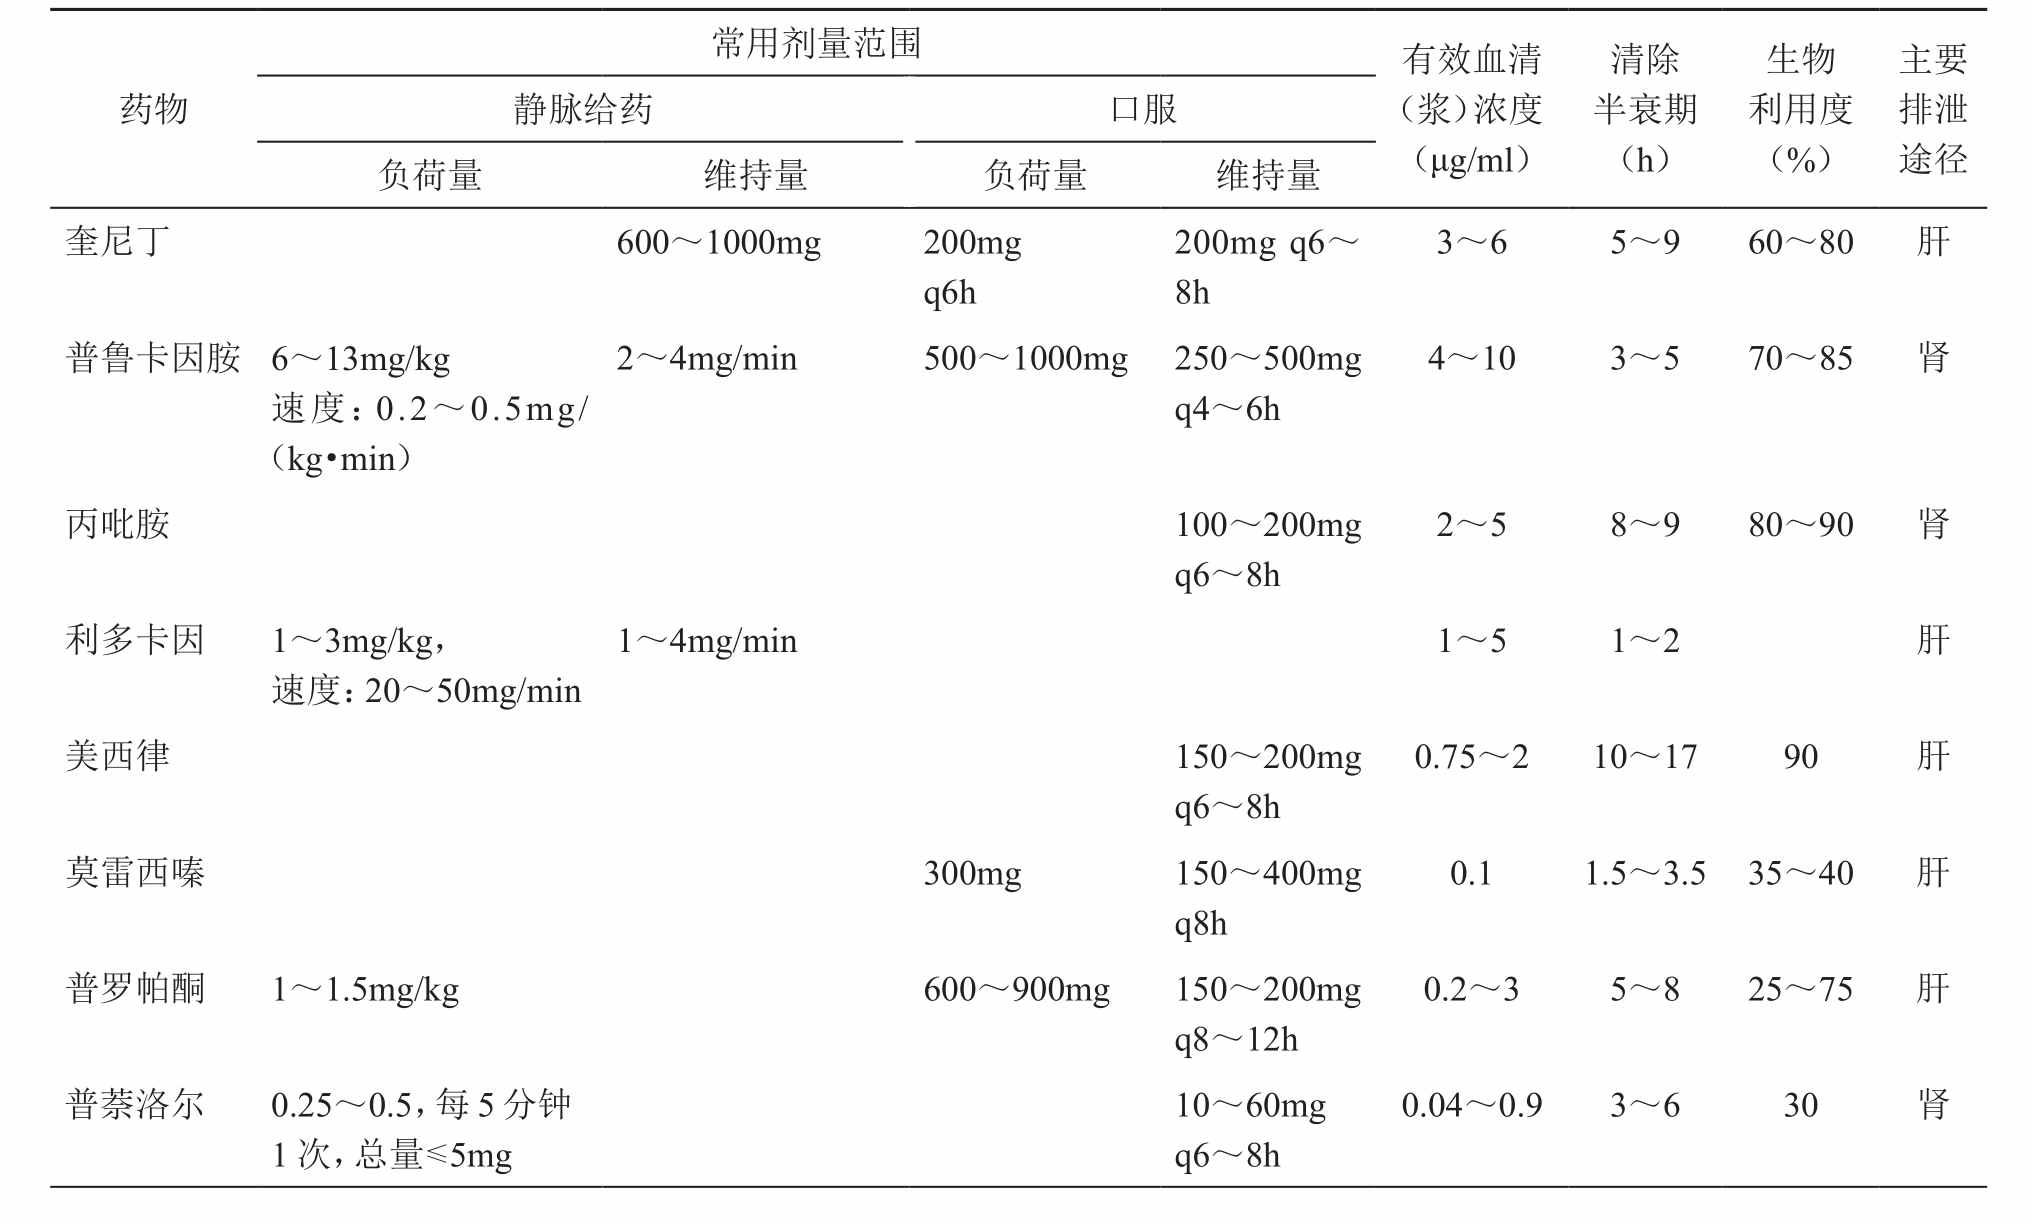
\includegraphics[width=\textwidth,height=\textheight,keepaspectratio]{./images/Image00572.jpg}\\
 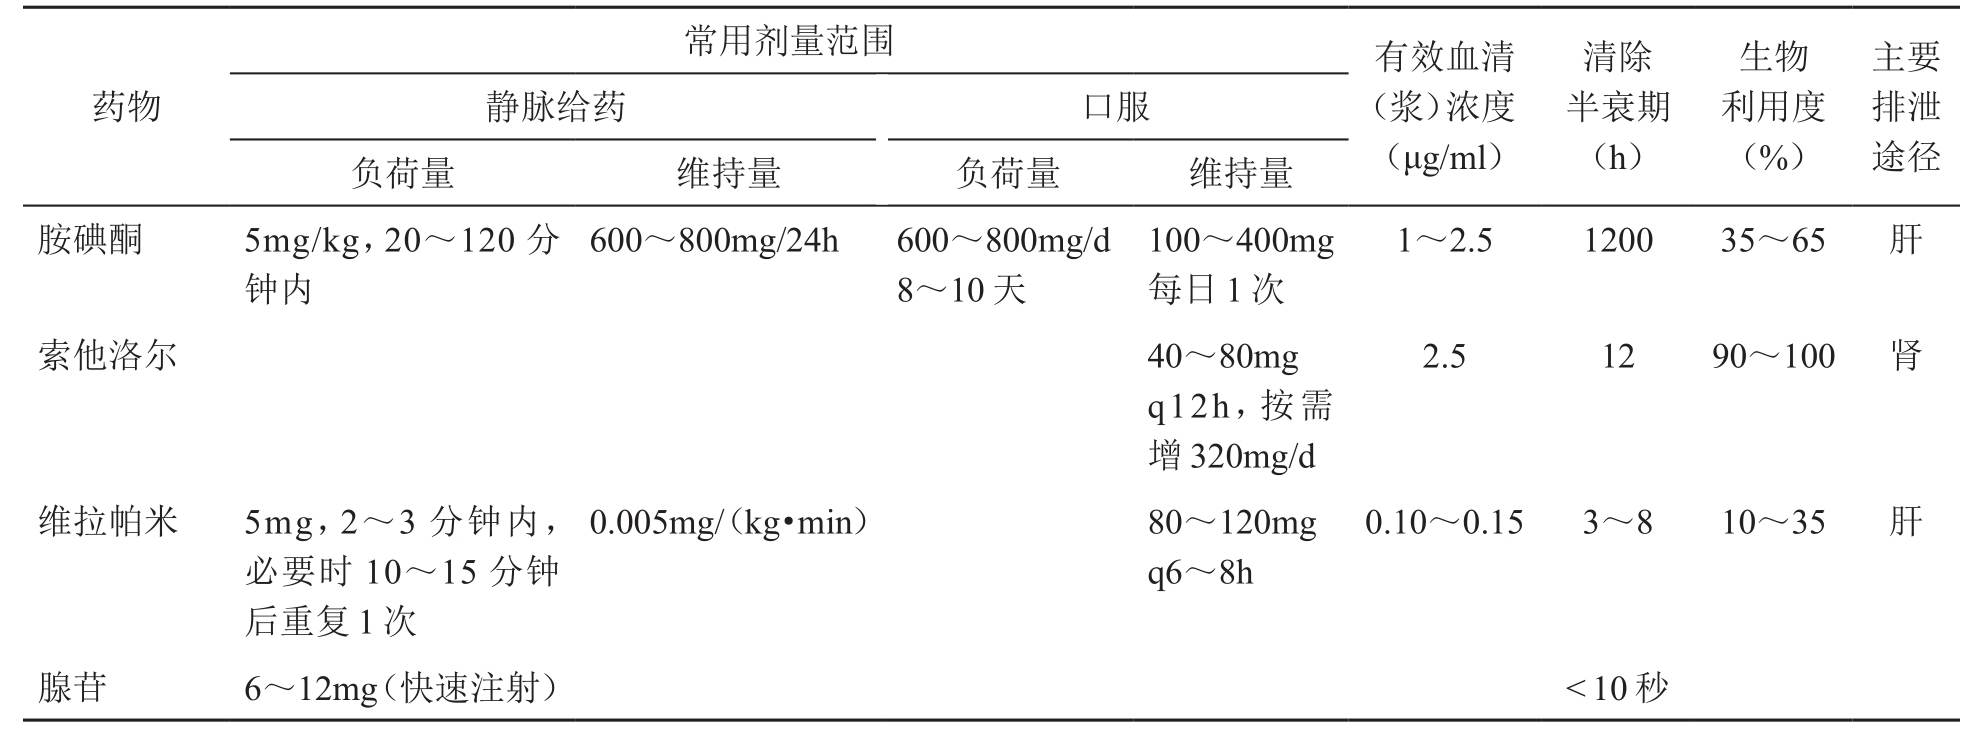
\includegraphics[width=\textwidth,height=\textheight,keepaspectratio]{./images/Image00573.jpg}
 \end{longtable}

\protect\hypertarget{text00422.html}{}{}

\section{抗心律失常药的临床应用}

\subsubsection{抗心律失常药的应用原则}

理想的抗心律失常药,应具有疗效确切、使用方便、不影响正常兴奋传导、剂量与疗效相关明确、对其他非心血管系统无毒副作用等,但目前尚缺乏这一“理想”药物。在临床运用抗心律失常药治疗心律失常时必须遵循以下原则:①应尽量找出病因,包括基本疾病和诱发因素(如心力衰竭、休克、呼吸衰竭、感染、高血压、甲状腺功能亢进或减退、电解质与酸碱平衡紊乱等),并予以积极的针对性处理。②根据心律失常的病因、类型、血流动力学改变、临床症状及潜在危害性的不同,针对性选用作用机制、药代动力学、给药途径、剂量、用药时间不同的抗心律失常药,才能够达到(或提高)疗效。③抗心律失常治疗的基点为终止或预防心律失常的发作,故本次心律失常发作控制后即应考虑其预防措施。

有关抗心律失常药的临床选用,可参考表\ref{tab151-5}。

\subsubsection{抗心律失常药的联合应用}

对单一药物治疗无效或患者不能耐受药物毒副作用的顽固性心律失常,尤其是室性心动过速,可以联合应用抗心律失常药物。联用的目的是增强抗心律失常作用及(或)减少、减轻毒副作用。一般应避免同一种类药物同时使用,但有人基于Ⅰa类药物抗心律失常作用类似而副作用不同,甚至相反,主张Ⅰa类可联合应用,而减少各自剂量,易于患者耐受长期应用。如奎尼丁可引起腹泻而丙吡胺引起便秘,二者联用可能互相抵消副作用。常用的联合用药方案有Ⅰa
+Ⅱ类;Ⅰb +Ⅱ类;Ⅰa +Ⅰb +Ⅱ类;Ⅰa +胺碘酮;Ⅰb +胺碘酮;Ⅰc +胺碘酮等。

\begin{table}[htbp]
\centering
\caption{抗心律失常药的临床选用}
\label{tab151-5}
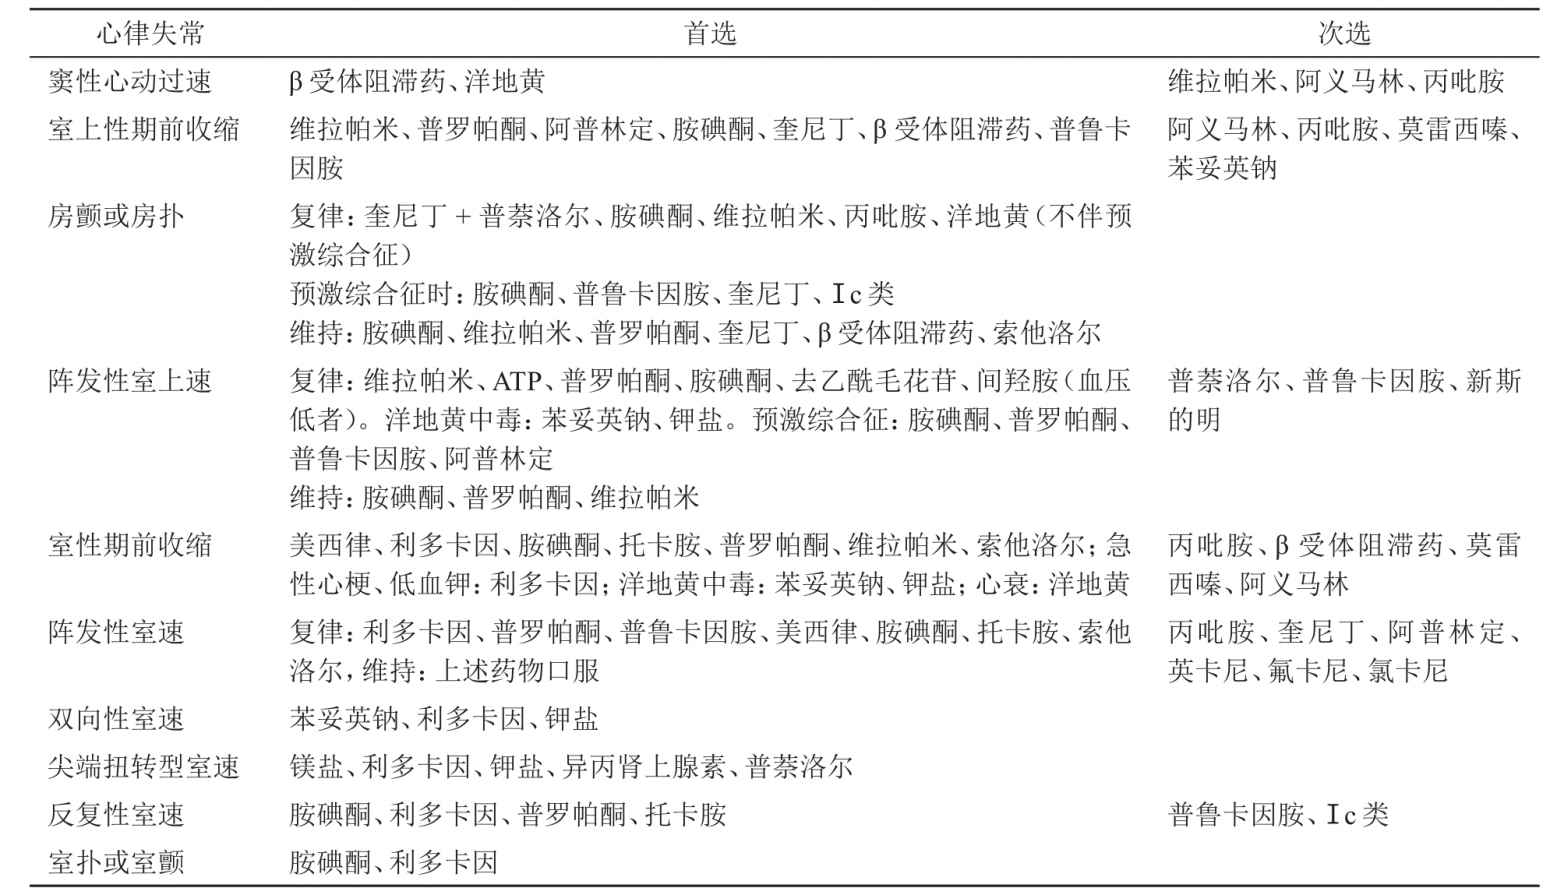
\includegraphics[width=6.65625in,height=3.82292in]{./images/Image00574.jpg}
\end{table}

临床应用经验较多的联合用药配对是奎尼丁和美西律。在治疗顽固的反复发作的持续性室速和室颤中,联合使用奎尼丁和美西律可使单独使用二者之一无效的心律失常得到满意控制;并且奎尼丁可使QT延长,而美西律使QT缩短,二药联合运用时,奎尼丁所致的QT延长而出现的扭转型室速的发生率低于单独使用奎尼丁组。

在使用奎尼丁转复房颤时,为防止因奎尼丁的抗胆碱作用加快房室传导,使心室反应增快,应先用洋地黄或同时用β受体阻滞剂,控制心室率。但联合用药时,要注意药物相互间的代谢和血浓度的影响,如奎尼丁与洋地黄合用时,奎尼丁将洋地黄从周围组织中替代出来进入血中,并减少洋地黄排泄,使洋地黄血浓度增高,二者合用时,应减少洋地黄剂量。

\subsubsection{抗心律失常药治疗室性心律失常的新观点}

用抗心律失常药治疗室性心律失常旨在减少或消除室性心律失常的症状和(或)减少心律失常死亡率。但美国多中心心律失常抑制试验(cardiac
arrhythmia supression
trial,CAST)的结果却显示:①使用Ⅰc类药物恩卡尼和氟卡尼对症状较轻、轻~中度心功能不全的心梗后患者行抗室性心律失常治疗,心律失常的死亡和猝死反较安慰剂组高3.6倍,总死亡率高25倍。②大部分死亡发生于室性心律失常被抑制时。CAST(Ⅱ)的莫雷西嗪也使死亡率增加。这些抗心律失常药致心律失常作用与用药时交感神经张力增高、左心室功能进一步恶化、传导缓慢及心肌缺血加剧等有关。有鉴于此,目前认为:

1.CAST的重要性在于提示并非所有的室性心律失常均需药物治疗,对室早即使能抑制也未必有益,故室性心律失常有良性、潜在恶性和恶性(致命性)之分,是否应用抗心律失常药及如何应用药物均应根据此危险/益处比而定:

(1)
良性室性心律失常(无器质性心脏病、无血流动力学障碍所致症状、猝死可能性极低的室早):可无需治疗;有症状予以镇静剂及β受体阻滞药;仍无效的用Ⅰc类药物。

(2)
潜在恶性心律失常(中或重度器质性心脏病,无血流动力学障碍的症状,左室射血分数≥0.30,中~重度猝死危险的频发室早和非持续性室速):可酌情予以β受体阻滞药。除了无血流动力学的症状外,潜在恶性与恶性心律失常基本相同。非持续性室速虽无即刻血流动力学改变,但左室功能不全及晚电位阳性,为潜在性恶性心律失常的最严重类型。

(3)
恶性(致命性)心律失常:主要为持续性室速和(或)室颤,又有“致命性室性心律失常”与“慢性致命性室性心律失常”之分:前者指患者就诊时室速(持续性单形性或尖端扭转性)或室颤伴显著血流动力学改变(严重的心脑功能不全),需立即予以药物、心电复律、起搏等治疗;后者指药物应用主要是为了预防,即减少或消除致命性心律失常的发生。对于致命性心律失常,应先予以Ⅰc类药物,并试用胺碘酮。

2.虽然室早既不能准确预报室速和室颤,亦非长期服药的适应证,但对心功能差(左室射血分数<
0.40)、复杂性室早、心室晚电位阳性、电生理检查诱发出持续性单形性室速者,均应长期服药。

3.抗心律失常药的早期致心律失常发生率
,心功能恶化及新发生的传导阻滞常与左室功能或药物种类有关;后期致心律失常的死亡率,左心室功能恶化可能并非主要,而与其药物特异作用有关。

4.Ⅰa和Ⅰc类对室性心律失常的治疗所致的负性肌力作用、严重的致心律失常作用,增加了心脏猝死和总死亡率;Ⅰb类的苯妥英钠、美西律、托卡胺的治疗死亡率亦较对照组有所升高。β受体阻滞药为目前唯一为大量资料证实的减少心梗后心律失常事件、心肌缺血发生率和预防猝死的一类药物,毒副作用少且几无致心律失常作用。Ⅲ类药物的胺碘酮和索他洛尔,近年已有多份资料显示可提高心梗后室性心律失常患者的生存率。Ⅳ类的维拉帕米已证实对心梗后室性心律失常或死亡率无明显影响。

5.需强调的是由于目前尚缺乏对良性和恶性心律失常的系统研究
,故不应过于简单片面地套用CAST的结果,室上性心动过速的治疗也不受其结果的影响。

\protect\hypertarget{text00423.html}{}{}

\section{抗心律失常药的致心律失常作用}

抗心律失常药物(ARRD)的致心律失常(proarrhythmia)是指用药后诱发既往未曾发生过的心律失常(provocation),或者使原有的心律失常恶化(aggravation)。所用药物的剂量或血浆药物浓度低于中毒水平,从而区别于药物中毒或过量导致的各种心律失常。确定促心律失常作用前需除外自身心律失常的恶化,以便确定停药或是加药。

ARRD的致心律失常作用大致可分为三类:①真正致心律失常作用(true
arrhythmogenesis);②促进或易化心律失常作用(facilitation);③显露致心律失常的新基础(unmasking
of a new
substrate)。第一类常指ARRD用药中出现新的心律失常(如应用奎尼丁致尖端扭转型室速),后两类指ARRD应用后或使自发的心律失常恶化,或显露隐匿基础所致新的心律失常。

\subsubsection{ARRD致心律失常作用的机制}

ARRD的致心律失常作用的有关电生理机制为:①几乎所有ARRD均抑制窦房结功能,并致窦房阻滞;②不同类型的ARRD对房室结传导影响不同,可致血流动力学明显的有害改变;③Ⅰa类使QT间期延长,心室肌不应期离散度增大,复极不均一而致折返;④Ⅰc类药物使室内传导缓慢,程度不均一,抑制传导的作用大于不应期延长而使原折返持续存在或产生新的折返;⑤氟卡尼、胺碘酮使心室颤阈改变;⑥奎尼丁、普鲁卡因胺、普萘洛尔、维拉帕米等静脉注射可引起起搏阈值升高使人工起搏失败,发生心动过缓及过缓依赖性心动过速;⑦氟卡尼、丙吡胺诱发慢性心力衰竭、奎尼丁致低血压等,均恶化血流动力学;⑧某些ARRD可诱发触发活动;⑨ARRD的负性肌力作用,为致心律失常作用提供基础。

ARRD致心律失常作用还可能与以下因素有关:特异质者;有持续性室速、室颤史者;电解质失衡(低血钾、低血镁);药物致自主神经功能改变;血流动力学恶化;心电图QT间期延长;心内传导延长;继发的心功能抑制;器质性心脏病;药物间的相互作用与药物浓度改变;治疗起始量较大和(或)快速增加剂量;药物代谢及排泄改变等。例如:肾脏疾病时,普鲁卡因胺、N-乙酰普鲁卡因胺、d-索他洛尔的血浓度升高而诱发Tdp;肝功能减退时,利多卡因的血浓度升高,会诱发室速或缓慢性心律失常;低血钾、低血镁使QT间期延长,易诱发Tdp,高血钾时,传导减慢,诱发缓慢性心律失常;心肌缺血时,Ⅰ类药使死亡率增加;普萘洛尔升高利多卡因血浓度,胺碘酮升高地高辛的血浓度,易诱发缓慢性心律失常。

\subsubsection{ARRD致心律失常作用的分类与诊断}

ARRD致心律失常作用有原发性和继发性之分:原发性指与基础心律失常和器质性心脏病以外其他任何可识别的致心律失常因素无关;继发性指发生需调节因素(血药浓度过高、药物相互作用、电解质紊乱、心肌缺血等)参加。按时间上分为早期药物治疗(<
30天)和晚期药物治疗(长期服药)。

用药后QT间期延长引起扭转型室速是较特异的促心律失常现象,但以某一种心律失常的量变来判断就很困难。80年代初提出过以室性期前收缩次数增加来判断,原10次/小时用药后增加10倍,1000次/小时增加2倍,或非持续性室速连续增多10倍及以上为促心律失常作用,或者室性期前收缩在用药前1~50次/小时、51~100次/小时、101~300次/小时、>
300次/小时,分别增加10、5、4、3倍等为促心律失常作用。现在认识到,室性期前收缩本身有较大波动,加上受病情变化的影响,这些定量标准已不可靠。

1998年国外部分专家认为,促心律失常不仅表现为快速心律,也可有缓慢型心律失常,部位除心室外,心房、房室结及窦房结水平均可发生,据此提出一新的促心律失常作用共识,介绍如下:

\hypertarget{text00423.htmlux5cux23CHP17-4-5-2-1}{}
(一) 新出现的持续性心律失常

\paragraph{快速心律}

①扭转型室速,QT延长;②多形室速,QT正常;③室颤;④持续性单形室速,间歇性发作;⑤持续性单形室速,不间断性;⑥房扑,1∶1传导。

\paragraph{心动过缓及传导障碍}

①窦房结功能低下;②房室阻滞;③明显的QRS增宽。

\hypertarget{text00423.htmlux5cux23CHP17-4-5-2-2}{}
(二) 原有心律失常恶化

1.室速由非持续性转变为持续性。

2.心动过速频率加快。

药物引起QT间期延长,尤其在低血钾或心动过缓时,可发生特异的扭转型室速。各种因素增加细胞内钙离子浓度,可能诱发后除极电位的触发活动,导致室速或室颤。促心律失常作用的发生明显受整体心脏状况和肝肾功能的影响。如奎尼丁引起的猝死是安慰剂的2~3倍,主要发生在心功能障碍患者,很少见于正常心脏。在肝功能衰竭时,扭转型室速也可增加。Podrid等报道,Ⅰ类药在LVEF
< 35\%和> 35\%患者中促心律失常分别为43\%
和26\%。Ⅰc类药明显减缓室内传导,可能造成新的室内折返途径,引起不间断性室速。在心肌缺血或明显心肌肥厚、心脏扩大时,加重正常与病变心肌间不均匀的复极和传导,产生新的折返,出现单形室速或扭转型室速。所以Ⅰ类药不宜用于明显心肌缺血和心功能障碍者。Ⅲ类药中胺碘酮虽延长复极和QT间期,但急性心肌梗死或心衰临床试验证实,其扭转型室速发生率仅不及1\%。索他洛尔的促心律失常随剂量上升,每日剂量超过320mg,扭转型室速发生率明显增加。Ⅰc类药物用于控制房颤或房扑时,可以延长房内传导,减少心房频率,或者使房颤转变为房扑,反而造成更多的心房激动下传,出现1∶1房室传导,加快心室率。

促心律失常多发生在开始用药24~48小时,72小时后渐为减少。若使用易于发生促心律失常的药物,特别是有心肌功能障碍或有诱因的患者,宜于医院内开始给药。胺碘酮起效缓慢,促心律失常现象不严重,可在门诊严密观察下给药。药物血浆浓度变化范围较大,除了有中毒可能性时,测定血药浓度指导用药并不实用。应强调严格掌握抗心律失常药物的适应证。

发生促心律失常时应及时停药,测定血浆电解质浓度,包括血钾和血镁,并按具体心律失常处理。必要时可心室起搏,严重血流动力学障碍时可以电复律。Ⅰc类药造成的不间断性室速处理较难,可给乳酸钠或碳酸氢钠,必要时可试用利多卡因。

\subsubsection{ARRD致心律失常作用的检测}

\paragraph{临床观察}

由于致心律失常作用多见于ARRD用药1周内,故此时应特别注意有无心律失常的加重或新的心律失常出现,体表心电图QRS波增宽>
25\%时,有可能诱发室性心律失常;用药后QT间期延长,易发生尖端扭转性室速;典型的药源性尖端扭转性室速发生前,T波降低而U波增高,二者融合,U波振幅增高较QT间期绝对值的延长更能促发致心律失常作用。

\paragraph{24小时动态心电图监测}

此为诊断ARRD致心律失常作用的最重要的检测方法。

\paragraph{电生理检查}

以心内生理程序刺激法不但可评价ARRD的作用,亦用于其致心律失常作用的评估。

\subsubsection{ARRD致心律失常作用的处理}

一旦发生,处理十分棘手。一般应采取以下措施:①首先停用有关的ARRD;②无症状或症状尚能耐受且无潜在危险的致心律失常作用,只需停药观察,再酌情处理;③出现缓慢型心律失常伴有症状者,可给予阿托品、异丙肾上腺素或临时心脏起搏治疗;④尖端扭转型室速可应用硫酸镁等治疗;⑤洋地黄中毒者予以相应的处理;⑥血流动力学不稳定的快速型心律失常应给予电复律治疗。但不少病例需待药物从体内排出后,方可控制发作。

\subsubsection{避免ARRD致心律失常作用的预防措施}

\paragraph{使用前应采取的措施}

决定对患者是否使用抗心律失常药物之前,应当注意:①寻找导致心律失常的原因和诱因:如有无电解质紊乱和酸碱失衡,尤其是低血钾、低血镁和代谢性酸中毒等;有无未满意控制的心力衰竭;有无进行性的心肌缺血;有无引起或加重心律失常的药物如洋地黄、三环类抗抑郁药和抗心律失常药本身。纠正这些因素对于治疗和预防心律失常的作用十分重要,而不应单纯着眼于轮番使用各种抗心律失常药物。②判断患者可能从抗心律失常药物治疗得到的益处与患者可能承受的风险和毒副作用的比例:一个AMI患者出现室早,应积极使用利多卡因或普鲁卡因胺加以消除;而一个心功能良好、甚至临床找不到器质性心脏病证据的患者,出现少数室性期前收缩,长期使用抗心律失常药物,药物的毒副作用远远超过心律失常本身,此时不需要用抗心律失常药物。

\begin{table}[htbp]
\centering
\caption{抗心律失常药物常见的药物相互作用}
\label{tab151-6}
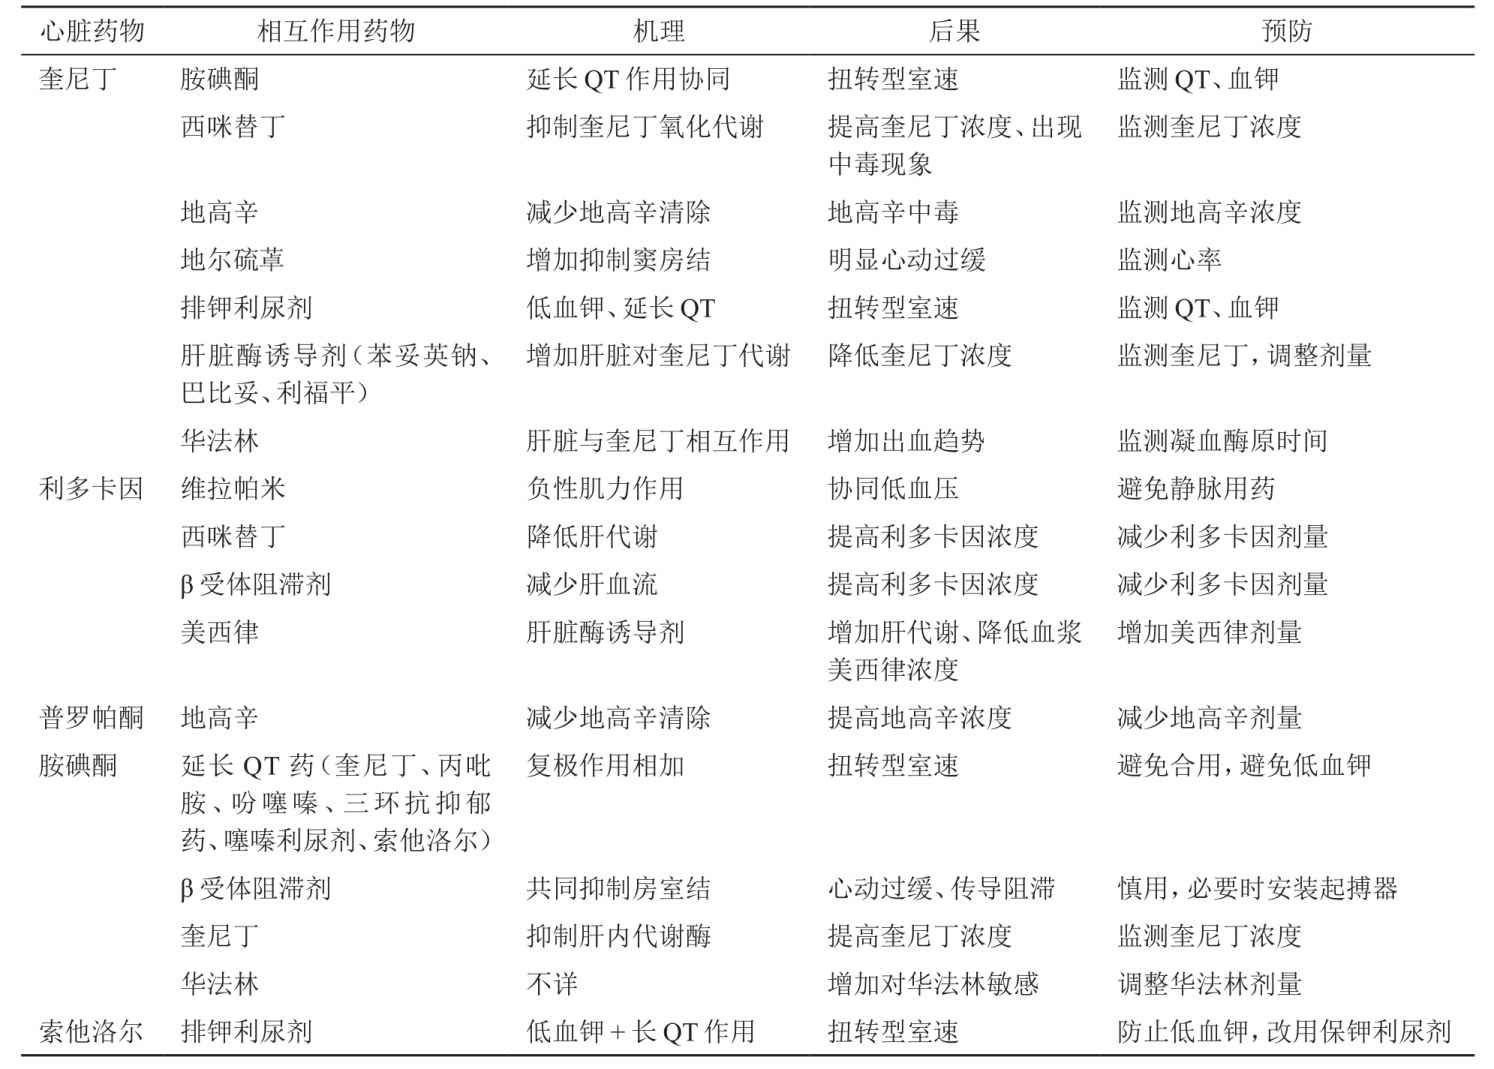
\includegraphics[width=6.625in,height=4.73958in]{./images/Image00575.jpg}
\end{table}

\paragraph{使用中的预防措施}

①如有条件,将服用奎尼丁患者短期收住院观察;②对于有器质性心脏病、心脏扩大和心功能不全者,对于高龄患者,使用Ⅰc类药物时应从小剂量开始;进行剂量调整时,增加剂量的间隔时间应相对延长,有条件时,应监测药物的血浓度;在变更剂量时,进行动态心电图监测,以便及早发现心律失常加重;如单一使用药物有效,尽量避免联合使用抗心律失常药物;严重的室速,应作电生理检查,进行药物筛选,可发现某些抗心律失常药的致心律失常作用,因此避免使用该药。抗心律失常药物常见的药物相互作用见表\ref{tab151-6}。

\protect\hypertarget{text00424.html}{}{}

\hypertarget{text00424.htmlux5cux23CHP17-4-6}{}
参 考 文 献

1. 陈新谦,金有豫,汤光.新编药物学.第17版.北京:人民卫生出版社,2011

2. Roden DM,Anderson ME. Proarrhythmia. Handb Exp
Pharmacol,2006,171:73-97

3. 中华医学会心血管病分会
,中华心血管病杂志编委会,抗心律失常药物治疗专题组.抗心律失常药物治疗建议.中华心血管病杂志,2001,29(6):323-336

4. Goldschlager N,Epstein AE,Naccarelli GV,et al. A practical guide
for clinicians who treat patients with amiodarone:2007. Heart
Rhythm,2007,4(9):1250-1259

\protect\hypertarget{text00425.html}{}{}

\hypertarget{text00425.htmlux5cux23CHP17-4-7}{}
附:胺碘酮抗心律失常治疗应用指南(2008)

中华医学会心血管病学分会 中国生物医学工程学会心律分会

胺碘酮抗心律失常治疗应用指南工作组

胺碘酮(amiodarone)是目前最常用的抗心律失常药物之一,自2004年制订《胺碘酮抗心律失常治疗应用指南》以来,又有不少新的相关指南和新的循证依据公布,且国内应用经验也日益丰富,为此必须对原指南加以修订,以便与当前的共识相一致。

\subsection{药理与电生理作用机制}

胺碘酮是以Ⅲ类药作用为主的心脏离子多通道阻滞剂,兼具Ⅰ、Ⅱ、Ⅳ类抗心律失常药物的电生理作用。包括:①轻度阻断钠通道(Ⅰ类作用),与静息态和失活态钠通道亲和力较大,与激活态钠通道亲和力小,使其从失活态恢复显著延长,通道开放概率减少,表现电压和使用依赖阻滞(在较小负向钳制电压、较快除极频率时阻滞作用加强),但没有Ⅰ类抗心律失常药物的促心律失常作用。②阻断钾通道(Ⅲ类作用)。胺碘酮可同时抑制慢、快成分的延迟整流钾电流(I\textsubscript{Ks}
、I\textsubscript{Kr} ),特别是开放状态的I\textsubscript{Ks}
。此外,胺碘酮还可阻滞超快激活的延迟整流钾电流(I\textsubscript{Kur}
)和内向整流钾电流(I\textsubscript{Kl}
)。③阻滞L型钙通道(Ⅳ类作用),抑制早期后除极和延迟后除极。④非竞争性阻断α和β受体,扩张冠状动脉,增加其血流量,减少心肌耗氧,扩张外周动脉,降低外周阻力。胺碘酮有类似β受体阻滞剂的抗心律失常作用(Ⅱ类作用),但作用较弱,因此可与β受体阻滞剂合用。就整体电生理而言,胺碘酮延长动作电位时程,但基本不诱发尖端扭转型室性心动过速(室速)。这是因为胺碘酮虽可延长心房和心室的动作电位时程,但不诱发后除极电位,不增加复极离散。胺碘酮阻滞肥厚心肌细胞I\textsubscript{Na}
、I\textsubscript{Ks}
的敏感性大于正常心肌细胞,阻滞I\textsubscript{Ca-L}
、I\textsubscript{to} 、I\textsubscript{Kl}
的敏感性又低于正常心肌细胞。胺碘酮对电重构的肥厚心肌细胞急性电生理反应有利于其在抗心律失常中的应用。静脉注射胺碘酮显示,Ⅰ、Ⅱ、Ⅳ类的药理作用较快,Ⅲ类药理起效时间较长。

胺碘酮的电生理作用主要表现在抑制窦房结和房室交界区的自律性,减慢心房、房室结和房室旁路传导,延长心房肌、心室肌的动作电位时程和有效不应期,延长旁路前向和逆向有效不应期。因此它有广泛的抗心律失常作用,可抗心房颤动(房颤)和心室颤动(室颤),可治疗房性心动过速(房速)和室速,也可治疗房室结折返性心动过速和房室折返性心动过速等。尽管胺碘酮延长QT/QTc间期,但尖端扭转型室速不常见(发生率<
1\%)。胺碘酮的多种电生理作用使其成为一广谱抗心律失常药。

胺碘酮药代动力学复杂。口服生物利用度平均为50\%(变化范围22\%~86\%),血药浓度和剂量呈线性相关。胺碘酮具有高度脂溶性,广泛分布于肝、肺、脂肪、皮肤及其他组织,分布容积大(可达60L/kg);主要通过肝脏细胞色素P450系统代谢,经粪便排泄;几乎不经肾脏清除(尿排泄<
1\%),故可用于肾功能减退的患者且无需调整剂量。胺碘酮口服起效及清除均慢,口服需数天至数周起效。静脉注射后由于胺碘酮从血浆再分布于组织中,血浆中药物浓度下降较快。胺碘酮清除半衰期长,长期用药在停药后3~10天血浓度降低至初始浓度的50\%。之后随着组织储存药物的排出进入较长的终末半衰期,可持续13~142天。胺碘酮主要代谢产物去乙基胺碘酮亦具有药理活性,且比胺碘酮的清除半衰期更长。胺碘酮和去乙基胺碘酮的血药浓度与治疗有效性和副作用之间没有相关性。

\subsection{临床应用}

\subsubsection{在房颤和心房扑动(房扑)中的应用}

房颤是最常见的心律失常,而且患病率随着年龄增长。中国房颤患者在年龄分布、病因及相关因素、房颤类型、脑卒中危险因素等流行病学特点与国外报道相似。房颤虽不即刻导致生命危险,但可造成程度不同的症状及血流动力学障碍,尤其伴有明显器质性心脏病时可能使心脏功能恶化,出现低血压、休克或心力衰竭(心衰)加重。在有危险因素的患者中易发生血栓栓塞。房颤根据发作情况分为初发性、阵发性、持续性及永久性。

房颤的药物处理策略为:①将房颤转复并维持窦性节律(节律控制);②不转复房颤,控制心室率(室率控制)。近年来非药物治疗房颤不断取得进展,但药物仍是多数房颤患者的主要治疗措施。虽然四类抗心律失常药对房颤都能起到不同的治疗作用,但以胺碘酮循证医学的资料最丰富。与其他药物或安慰剂对比,胺碘酮对房颤的转复、防止复发、维持窦性心律(窦律)的总体疗效较其他药物为好,且负性肌力作用和促心律失常作用少,故适用于多种临床情况。多中心临床试验证明,在急性心肌缺血、急性心肌梗死或心功能不全时,当其他抗心律失常药属于禁忌时,推荐应用胺碘酮,故此成为重症情况合并房颤时的首选药物。

\paragraph{用于转复房颤}

已经有多项临床研究证实,胺碘酮可转复新近发生的房颤,其转复作用优于安慰剂,房颤持续时间超过48小时者益处更明显。但就即刻转复房颤的作用,胺碘酮并不优于多非利特、氟卡尼或普罗帕酮。因此房颤指南中将其作为转复房颤的备选药物(Ⅱa类推荐、证据水平A)。需在短时间转复房颤者,可选用静脉胺碘酮。血流动力学稳定、已超过48小时的房颤,可选胺碘酮口服。房颤已超过7天以上者,药物转复成功率降低,此时胺碘酮常用作电复律的准备用药,通常选静脉或口服胺碘酮。如不能转复,施行电复律,由此增加电复律成功机会,并减少电除颤次数,复律后又可减少房颤复发,维持稳定窦律。胺碘酮配合电复律为房颤复律的Ⅱa类推荐、证据水平B。

\paragraph{用于房颤后维持窦律}

目前胺碘酮是用于房颤转复后维持窦律的最常用的药物。由于临床试验中所选房颤的类型、年龄、心脏病等情况及病程不同,胺碘酮在房颤复律后维持窦律结果的可比性差。多项临床试验及荟萃分析显示,胺碘酮在维持窦律方面优于其他抗心律失常药物。国内研究亦显示,胺碘酮维持窦律的1年有效率为67.5\%~71.8\%。AFFIRM亚组研究显示,在维持窦律方面,胺碘酮明显优于索他洛尔和Ⅰ类抗心律失常药物。虽然药物引起的不良反应比较常见,但在中途停药及促心律失常方面,胺碘酮少于Ⅰ类抗心律失常药物。房颤复律后是否长期用胺碘酮维持窦律,取决于多种因素。房颤频发者或不用药物不能保持窦律者,需长期用胺碘酮。对于初发房颤,不论自发终止或复律终止,都不主张加用胺碘酮。由于胺碘酮的心外副作用多,长期应用应先进行效益-风险评估。胺碘酮不用于房颤的一级预防。

鉴于AFFIRM研究发现,在特定的人群中,节律控制与室率控制在脑卒中、生活质量、死亡率方面差异无统计学意义,故在应用抗心律失常药物维持窦律时一定要衡量效益-风险比。胺碘酮主要用于有明显器质性心脏病、有症状房颤患者的窦律维持。房颤指南建议用于明显左室肥厚和慢性心衰患者。若是应用某个维持量仍有发作,可在短期内适当增加剂量(再负荷),以后给予新的维持量。用胺碘酮期间,如果房颤仅偶有发作,发作时频率不快,且持续时间不长,不应视为失败,可以继续用原剂量维持。

\paragraph{用于控制房颤心室率}

房颤不能转复为窦律或无需转复时,应该将心室率控制到合理范围。在无禁忌证患者,急性期首选的药物是静脉β受体阻滞剂或钙拮抗剂。伴有心功能降低的重症患者,洋地黄制剂及胺碘酮可以作为首选。静脉应用胺碘酮控制房颤心室率与地尔硫{}
疗效相当,低血压发生率较少。在其他药物控制无效或有禁忌时,静脉胺碘酮为Ⅱa类推荐。口服胺碘酮不适宜作为一线药物用于慢性房颤的室率控制。如果β受体阻滞剂、钙拮抗剂或地高辛(单独或联合应用)无效,房室结消融加起搏器也可选择。口服胺碘酮,虽然也可以降低快速房颤的心室率,但长期应用可能有一定副作用,因此在欧美及我国处理房颤的建议中,实际推荐类别仅为Ⅱa。

\paragraph{在预激综合征伴房颤中的应用}

小规模研究表明,静脉胺碘酮对于预激伴房颤有效,但应注意静脉用药后也有心室率加快导致室颤的报道。由于静脉胺碘酮起效相对慢,所以作用有限。此时电复律应作为首选。胺碘酮的长半衰期可能会影响心律失常病情判断和介入治疗决策的选择。对于长期治疗,胺碘酮适用于合并器质性心脏病且不宜行射频消融或其他措施无效时。血流动力学稳定的经旁路前传的房颤患者应用胺碘酮为Ⅱb类推荐。

\paragraph{在慢性心衰伴房颤中的应用}

胺碘酮不加重心衰并且有可能使其改善,产生促心律失常作用较其他药物小。慢性心衰抗心律失常生存研究亚组分析(CHF-STAT)评价了胺碘酮对慢性心衰患者房颤的作用,胺碘酮治疗组房颤转复较对照组更多见,房颤未转复者心室率明显减慢。接受胺碘酮治疗转复为窦律组的生存改善。基线为窦律者应用胺碘酮可减少新发房颤的出现。慢性心衰伴有症状性房颤,可考虑应用胺碘酮行节律控制,但属二线治疗,仅用于其他治疗不成功的病例,对于重症患者可静脉给药。慢性心衰合并无症状的房颤,衡量效益-风险比,应选择控制心室率的策略。

\paragraph{在急性心肌梗死伴房颤中的应用}

房颤可并发于急性心肌梗死,心室率多较快。原有房颤者发生急性心肌梗死,因交感兴奋和心功能不全也使心室率加快。二者室率控制都是基本治疗。此时心肌对洋地黄较敏感,应慎用洋地黄控制心室率,仅作为Ⅱa类推荐,而此时静脉应用胺碘酮减慢心室率为Ⅰ类推荐。

\paragraph{与 β受体阻滞剂联合在房颤中的应用}

胺碘酮与β受体阻滞剂合用,心脏性死亡、心律失常及猝死的相对危险均可能较单用其一者低。用药后心率减慢程度不因合用β受体阻滞剂而更明显,但应监测心率变化。已有其他指征使用β受体阻滞剂的患者,发生房颤需要加用胺碘酮,一般无需停用β受体阻滞剂。

\paragraph{与血管紧张素Ⅱ受体拮抗剂联合在房颤中的应用}

临床试验发现,胺碘酮与血管紧张素受体拮抗剂厄贝沙坦合用,可使维持窦律者明显增多,房颤未复发者的生存率明显高于复发者。其他血管紧张素Ⅱ受体拮抗剂也应有类似的效应。

\paragraph{在房扑中的应用}

房扑和房颤常合并存在,典型(Ⅰ型)房扑是大折返性房性心律失常,心房率为250~350
次/分,常呈2∶1房室传导。房扑心室率较难控制,通常需要较高的药物剂量,甚至两种或多种房室结阻滞剂联用。几项研究已经证实胺碘酮对于房扑患者维持窦律的有效性和安全性,但治疗的病例有限。治疗Ⅰ型房扑,射频消融优于胺碘酮和其他抗心律失常药物。

\subsubsection{在其他快速室上性心律失常中的应用}

几项小规模的临床研究提示,胺碘酮可终止多源性房速。成人及儿童中已证实,胺碘酮可终止加速性交界区自主心律。也可终止慢性持续性房速,并减少由此产生心动过速性心肌病的可能。胺碘酮终止房室结折返性心动过速和房室折返性心动过速有效,但应选择疗效更快或毒性作用小的药物。长期治疗尽管有效,但难以控制复发,应选择导管消融进行根治。

\subsubsection{在快速室性心律失常的应用}

\hypertarget{text00425.htmlux5cux23CHP17-4-7-2-3-1}{}
(一) 用于快速室性心律失常的急性期治疗

1.胺碘酮在血流动力学稳定的单形性室速
、不伴QT间期延长的多形性室速和未能明确诊断的宽QRS心动过速治疗中应作为首选。在合并严重心功能受损或缺血的患者,胺碘酮优于其他抗心律失常药,疗效较好,促心律失常作用低。虽然有报道,胺碘酮可以使持续性室速终止,但室速持续时间过长或血流动力学不可耐受时,应进行电复律。本药的主要功效是预防复发,这种作用可能需要数小时甚至数日才能达到。当口服胺碘酮剂量过低而导致室性心律失常复发时,若病情紧急者,可行静脉再负荷。再负荷后的静脉维持用法与初始用法基本相同。可以一直用到心律失常控制并开始新的口服维持量。

2.在心脏骤停中的应用
在电复律及注射肾上腺素无效的院外发生的心脏骤停患者中,胺碘酮已被证明可以改善电除颤效果,从而改善心肺复苏患者的入院存活率。胺碘酮的此种作用优于利多卡因。但现在还没有改善出院存活率的证据。在无脉性室速或室颤造成心脏骤停时,经常规心肺复苏、应用肾上腺素和电复律无效的患者,在坚持进行心肺复苏的前提下应首选静脉注射胺碘酮,然后再次电复律。

3.在“电风暴”中的应用
“电风暴”指持续室速或室颤、24小时内发作≥2次,通常需要电转复。这种顽固的心律失常不但危及患者的生命,而且可使已置入的起搏除颤器(ICD)频繁工作,造成电源快速耗竭和患者的痛苦。小规模非随机研究证实,胺碘酮对于其他药物治疗无效的反复发作的持续性室性心律失常有效。对心肌梗死后患者的电风暴,在应用交感神经阻滞剂之后使用胺碘酮比使用其他抗心律失常药物更能降低短期病死率。尽管研究病例有限,但胺碘酮合用β受体阻滞剂被认为是治疗电风暴最有效的方法。

\hypertarget{text00425.htmlux5cux23CHP17-4-7-2-3-2}{}
(二) 在缺血性及非缺血性心脏病心脏性猝死一级预防中的应用

对有器质性心脏病同时伴有频发室性期前收缩(室早)和短阵室速的患者,特别是复杂室早伴有心功能不全者是发生猝死的高危人群。荟萃分析显示,胺碘酮可使总病死率明显下降,但临床试验(如CAMIAT和EMIAT没有证实胺碘酮能够减少这类患者的总病死率,但可明显减少心律失常死亡。心肌梗死后心功能正常的患者应用胺碘酮作用非常有限。但有研究显示,β受体阻滞剂能降低猝死及心肌梗死后总病死率,故预防用药首选β受体阻滞剂。

在缺血性心脏病猝死一级预防几项前瞻性临床研究中(MADITⅠ、MUSTT、MADITⅡ、SCD-HeFT),比较了ICD与抗心律失常药物的应用。在非缺血性心肌病猝死一级预防中也进行了几项研究(CAT、AMIOVIRT等)。以上研究均证实,在降低总死亡率方面,ICD明确优于抗心律失常药物。发生于器质性心脏病患者的非持续性室速,如果患者有明显左心功能不全或电生理检查诱发出伴有血流动力学障碍的持续性室速或室颤,应该首选ICD。没有条件置入ICD者用药物治疗,首选胺碘酮。如果电生理检查不能诱发持续性室速,治疗主要针对病因和诱因。在此基础上,应用β受体阻滞剂有助于改善症状和预后。对于上述治疗措施效果不佳且室速发作频繁、症状明显者可用胺碘酮预防或减少发作。

\hypertarget{text00425.htmlux5cux23CHP17-4-7-2-3-3}{}
(三) 在心脏性猝死二级预防中的应用

在一项早期的临床试验中
,心脏骤停幸存者经验性应用胺碘酮与电生理试验指导的传统抗心律失常药物减少室性心律失常的复发,改善院外发生心脏骤停后存活患者的长期生存。但后来进行的AVID研究显示,ICD较其他抗心律失常药物显著降低总死亡率。对于已经有恶性室性心律失常(无脉性室速、室颤)病史的患者,目前已明确心脏性猝死的二级预防应该首选ICD。在无条件或无法置入ICD的患者应该使用胺碘酮。单用胺碘酮无效或疗效不满意者可以合用β受体阻滞剂。即使不能完全控制心律失常的发作,但胺碘酮有可能使室速的频率明显减慢,变为血流动力学可以耐受的室速。

\hypertarget{text00425.htmlux5cux23CHP17-4-7-2-3-4}{}
(四) 作为ICD的辅助治疗

置入ICD的患者通常伴有器质性心脏病,频繁的心律失常发作会导致ICD反复放电,应该辅以药物控制。有指征有条件的患者也可考虑导管射频消融。Ⅰ类抗心律失常药物相对禁忌,胺碘酮和索他洛尔较常用。胺碘酮加β受体阻滞剂较索他洛尔或β受体阻滞剂单独应用减少ICD放电更有效。关于胺碘酮对ICD除颤阈值的作用,见“药物不良反应”部分。

\subsubsection{在急性冠状动脉综合征和心衰中的应用}

急性冠状动脉综合征时,由于缺血性心电不稳定可出现室早、室速、室颤或加速性室性自搏心律,也可出现各种室上性心律失常,胺碘酮是基本的选择。心衰时由于交感张力上升,肾素-血管紧张素-醛固酮系统活动增加,导致心电活动不稳定,因此发生房颤、室速或室颤的概率上升。如有心律失常发作,胺碘酮也是首选的药物,其安全性高于其他抗心律失常药物。但要注意胺碘酮与某些抗心衰的药物合用,尤其与利尿剂、洋地黄联合应用,有可能表现出促心律失常作用,甚至发生尖端扭转型室速。因此在心衰中应用胺碘酮要严观察、勤随访,尤应避免发生低钾血症。

\subsubsection{在心脏围术期的应用}

心脏手术(尤其是冠状动脉旁路术)后,房颤发生率达20\%~50\%,多发生于术后2~3天。近年有临床试验在手术前后用胺碘酮可减少房颤或房扑、快速室性心律失常、脑卒中的发生,并减少住院天数。大规模随机对照临床试验发现,胺碘酮明显降低术后快速房性心律失常。由于短期服用毒副作用较小,术后房颤患者在接受β受体阻滞剂治疗基础上保留胺碘酮是合理的。若无长期使用的指征,为减少胺碘酮的不良反应,在术后6~12周应停用胺碘酮。

\subsection{使用方法与剂量的建议}

由于胺碘酮的药效学、电药理学及药代动力学有诸多复杂的特征,针对不同的心律失常,其用药途径、方法和剂量均有不同的要求。

国内外都没有明确地统一过胺碘酮的使用剂量,这是因为该药的个体反应差异很大。年龄(老年用量小)、性别(女性用量小)、体重(体重轻用量小)、疾病(重症心衰耐量小)、心律失常类型(室上速、房颤用量小)及个体(相同条件的个体反应不同)均有差异,反映在使用剂量上也有差异。过去曾经使用较大的口服剂量(维持量在400~600mg/d),现在多偏向小剂量,以100~300mg/d维持,但在具体患者的治疗中仍可调整。维持治疗中没有特殊的原因不要过于频繁地调整剂量,每次调整需要较长(甚至达数月)的观察时间才能确定疗效和安全性。

静脉胺碘酮的使用剂量和方法也要因人而异。不同患者的剂量可有很大的差别,应根据心律失常的发作情况和患者的其他情况进行调节。静脉胺碘酮的使用最好不要超过3~4天,应特别注意选用大静脉,最好是中心静脉给药。胺碘酮静脉使用必须给予负荷量静脉注射,需要维持时应立刻给予静脉滴注。单纯使用小剂量静脉滴注不能在短时间内发挥作用。

大多数静脉应用胺碘酮的患者都需要继以口服治疗。目前没有严格的药理学试验指导静脉与口服的接替方法。原则上静脉应用的时间越长,剂量越大,口服的开始剂量越小。鉴于静脉使用胺碘酮的时间不宜太长,可以考虑从静脉使用的当天就开始口服,从常规负荷量起始。如果患者的情况不允许(如气管插管、意识不清等)可以延长静脉的使用时间直至具备口服的条件。

以下根据现有的国内外文献资料,提出不同的心律失常中胺碘酮口服和静脉的用法和用量范围,供临床应用参考。

\paragraph{室颤或无脉室速的抢救}

在心肺复苏中,如2~3次电除颤和血管加压药物无效时,立即用胺碘酮300mg(或5mg/kg)静脉注射,以5\%葡萄糖稀释,快速推注,然后再次除颤。如仍无效可于10~15分钟后重复追加胺碘酮150mg(或2.5mg/kg),用法同前。注意用药不应干扰心肺复苏和电除颤。室颤转复后,胺碘酮可静脉滴注维持量。在初始6小时以内以1mg/min速度给药;随后18小时以0.5mg/min速度给药;第一个24小时内用药总量(包括静脉首次注射、追加用量及维持用药)一般控制在2.0~2.2g以内。第二个24小时及以后的维持量根据心律失常发作情况酌情减量。

\paragraph{持续性室速}

对于血流动力学稳定的持续性单形、多形性室速和未明确诊断的宽QRS心动过速,首剂静脉用药150mg,用5\%葡萄糖稀释后推注10分钟。首剂用药10~15分钟后如仍不见转复可重复追加静脉150mg再负荷,用法同前。若使用了胺碘酮数次负荷后室速未能很快转复,应考虑电复律。此种持续室速有反复发作的可能,一般需要静脉维持用药,方法同前述室颤或无脉性室速。

\paragraph{恶性室性心律失常的预防}

用于无可逆原因引起的室颤或室速,在复律后、β受体阻滞剂无效的非持续性室速、置入ICD后均需应用胺碘酮预防复发。起始负荷量800~1600mg/d分次服用、共2~3周,宜在住院期内开始应用,也可参考房颤的治疗用量。维持量一般不宜超过400mg/d,女性或低体重者可减至200~300mg/d维持。有恶性室性心律失常病史的患者,口服胺碘酮不应过分强调小剂量。对已置入ICD者,合并应用小剂量胺碘酮(200mg/d)可以减少室颤或室速发作次数,降低室速的频率,使发作时的血流动力学变化易于耐受。

\paragraph{房颤的治疗与预防复发}

胺碘酮用于药物转复的口服剂量,住院患者1.2~1.8g/d分次口服,直至总量10g。院外患者600~800mg/d分次口服,直至总量10g。静脉用量,5~7mg/kg静脉注射30~60分钟,然后以1.2~1.8g/d持续静脉滴注或分次口服,直至总量达10g。

口服预防阵发性房颤发作或进行电复律的药物准备,可用较慢的负荷方法,如600mg分次服用、共7天,400mg分次服用、共7天,必要时增加剂量或延长负荷时间。电复律可在1周左右进行。口服维持量一般为200mg,可根据病情减至100mg/d或200mg/d、每周服药5天。

胺碘酮控制房颤心室率时的静脉用量方法与上述相似。

\subsection{药物不良反应}

胺碘酮的药理学特征复杂,作用多样,故可引起多种不良反应(附表1)。由于半衰期长,胺碘酮潜在的器官毒性比半衰期短的药物更严重,也更难处理。大多数不良反应经过减量或停药可以逆转。许多不良反应只要予以解释,解除患者的顾虑,严密随访观察即可。而重要脏器的毒性可能是严重的,需要更积极地处理。

附表1 胺碘酮的不良反应及处理

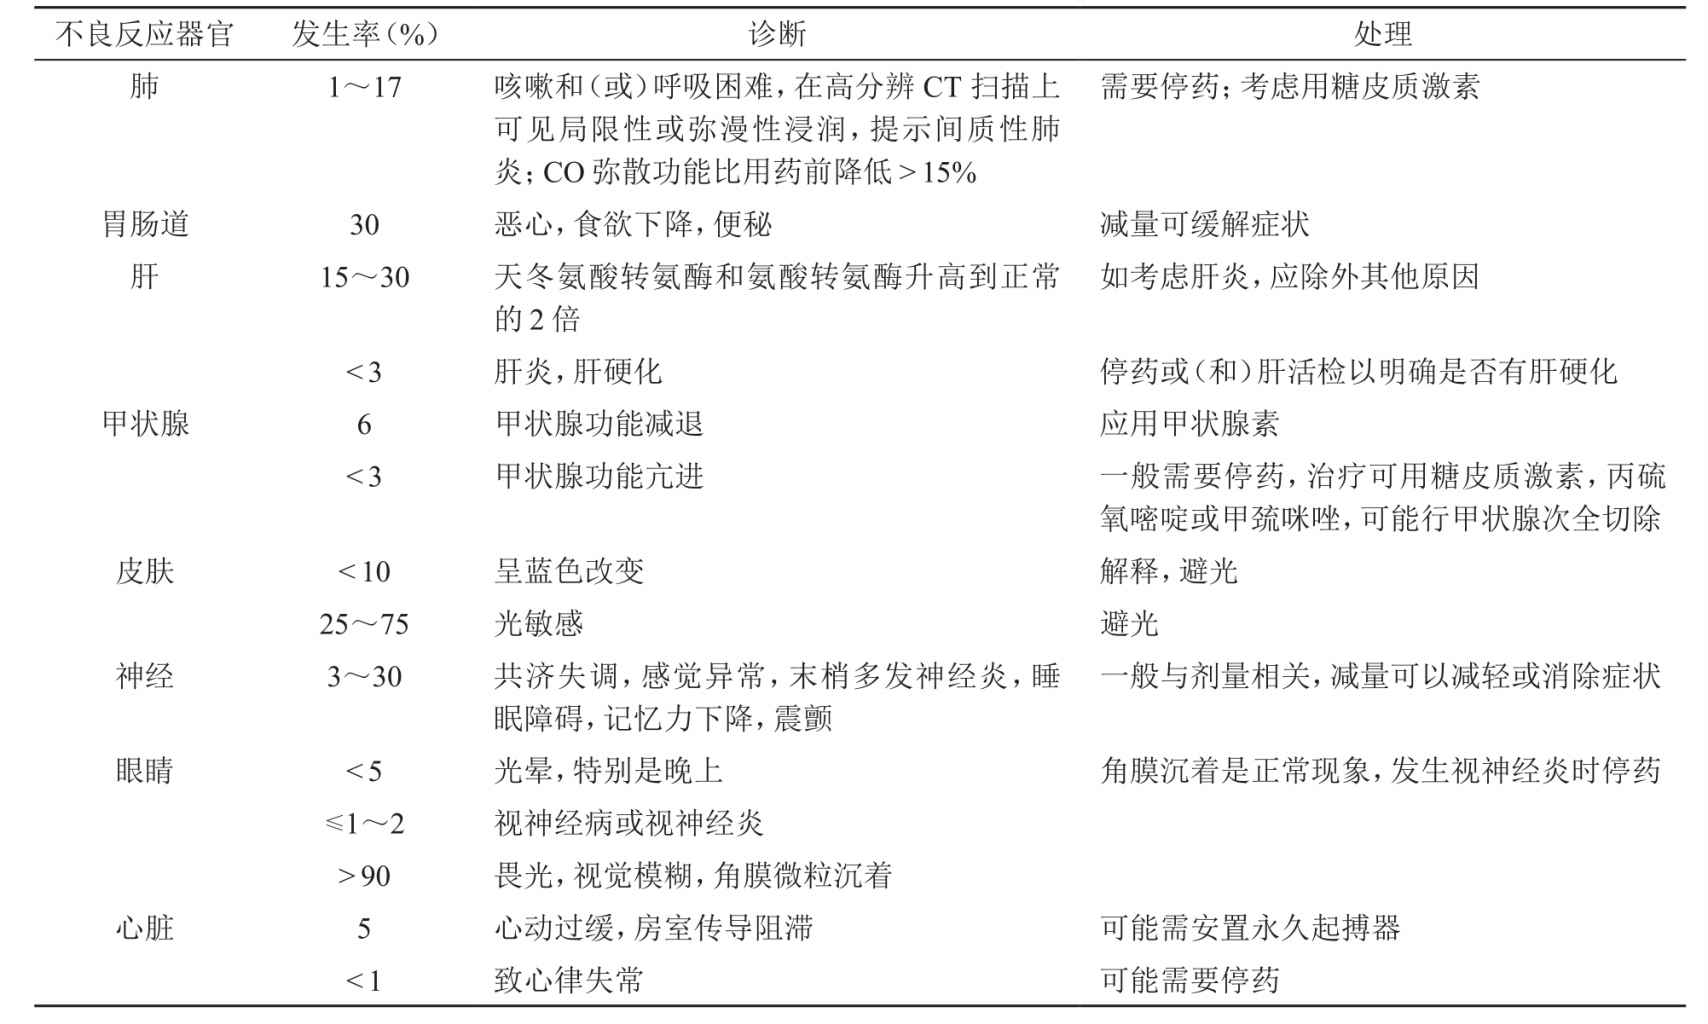
\includegraphics[width=6.66667in,height=4in]{./images/Image00577.jpg}

1.胺碘酮肺毒性的症状和体征缺乏特异性
,起病隐匿,最短见于用药后1周,多在连续应用胺碘酮3~12个月后出现。最早表现为咳嗽,但病情发展时可出现发热和呼吸困难。X线胸片或高分辨肺CT扫描显示局部或弥漫纤维化,一氧化碳弥散功能较用药前降低>
15\%,诊断可确定。支气管镜检查有助于除外结核、肿瘤播散等其他疾病。一旦出现肺部不良反应,应予停药,糖皮质激素治疗胺碘酮的早期肺毒性可能有效。肺毒性的早期表现可以类似于慢性心衰,因此高度警惕这一毒性作用是必要的。未能早期诊断肺毒性反应可能导致生命危险。目前临床实践中主张使用小剂量维持,肺毒性的发生率大大降低。

2.消化系统的不良反应
如恶心、食欲下降和便秘很常见,特别是在开始服用负荷量时容易出现,减量后服用维持量时症状通常可以缓解。最严重的消化系统不良反应是肝炎和肝硬化。静脉应用发生肝脏损害较口服多见。如丙氨酸氨基转移酶升高达2倍以上,应考虑肝炎的可能。诊断胺碘酮的肝脏毒性时应除外其他原因所致的肝功能异常,如其他药物、病毒、酒精等。如果确诊发生了胺碘酮肝脏毒性反应,应该停药。胺碘酮引起的肝炎可能是致命的。

3.甲状腺功能异常较常见 若仅有化验异常,如T\textsubscript{4}
、反T\textsubscript{3} 、促甲状腺激素(TSH)轻度升高、T\textsubscript{3}
水平轻度降低而无临床表现的患者,可加强监测而不需要特殊处理。甲状腺功能减退(甲减)的发生可能比较隐匿,其症状和体征易被误诊为其他原因所致,如心动过缓归因于胺碘酮本身或其他药物。随访中监测TSH很重要,T\textsubscript{3}
降低、TSH升高> 5μU/ml,应考虑为甲减;T\textsubscript{3} 升高、TSH下降<
0.1μU/ml,应考虑为甲状腺功能亢进(甲亢),但不同的化验室采用不同的免疫化学发光设备,会有不同的结果。甲减用左旋甲状腺易于治疗,使TSH正常化。而甲亢比较难处理。甲亢可加重房颤或出现快速室性心律失常,故应停用胺碘酮。由于碘化钠的吸收被胺碘酮分子中的碘化物抑制,所以不能进行\textsuperscript{131}
I放射治疗。胺碘酮所致的甲亢一般是甲状腺炎,所以糖皮质激素可能有效。丙硫氧嘧啶和甲巯咪唑可以作为间歇治疗措施。如果无法停用胺碘酮,可以考虑甲状腺次全切除术,以逆转甲亢。

4.皮肤
蓝灰色改变是长期服用胺碘酮的特征,通常在面部和眼睛周围最明显。这只表明有药物的吸收,日晒可使之加重。如有日光过敏,要告诉患者避免日晒,使用防晒用品。

5.神经系统异常
有小脑性共济失调、感觉异常(末梢神经炎)、睡眠障碍,偶尔有记忆力下降。往往与药量有关,减量即可减轻或消除症状。

6.裂隙灯检查可见角膜沉着,但仅反映药物吸收。光晕也很常见,一般不影响视力,应向患者解释,使之免除顾虑。最严重但很少见的并发症是视神经炎,一旦发生,必须停药。

7.心脏的不良反应比较少见
服药期间QT间期均有不同程度的延长,且可出现T波切迹、振幅下降,一般不是停药的指征。胺碘酮引起的QT间期延长是药物与组织结合的表现,不属药物不良反应,单纯由胺碘酮引发尖端扭转型室速不常见。如有扭转型室速发生,多有诱因,如低血钾、心动过缓或与其他可延长QT的药物合用等,因此必须注意消除诱因。

心动过缓是药物作用。对老年人或窦房结功能低下者,胺碘酮进一步抑制窦房结,窦性心率<
50次/分者,宜减量或暂停用药。偶尔需要永久心脏起搏。心室率、收缩功能不受影响。

胺碘酮常用于起搏器以及ICD置入术后的患者,以帮助控制房性和室性快速心律失常。服用胺碘酮不改变起搏阈值,但可使室速的心率减慢至ICD诊断的频率阈值以下,并能提高除颤阈值。因此已经置入ICD的患者服用胺碘酮时,完成负荷量之后应进行必要的检测,明确有无胺碘酮的不良影响,并及时调整ICD的相关参数。

静脉使用胺碘酮的主要副作用是低血压和心动过缓。减慢静脉推注速度、补充血容量、使用升压药或正性肌力药物可以预防,必要时采用临时性起搏。少数患者可出现明显的肝功能异常,需要停药并给予保肝治疗。静脉推注可诱发静脉炎,因此应选用大静脉,稀释后缓慢注射。

\subsection{用药随访}

静脉使用胺碘酮时,应注意观察疗效和可能出现的副作用,并做好详细的使用记录,内容包括当日静脉剂量、口服剂量、当日总剂量、累计剂量(从使用胺碘酮第一天开始累加的剂量)、血压、心率、心电图的重要指标(PR、QRS、QT、QTc间期等)以及一些重要的病情和实验室检查资料。定期进行各种化验室检查,特别注意复查肝功能。

对于服用胺碘酮的患者,应进行合理的长期随访,进行效益-风险比的评价。注意发现和预防严重副作用,出现副作用后要积极处理并加强随访。药物的副作用有一定程度的剂量相关性,且随用药时间的延长而增加。由于胺碘酮清除很慢,长期口服胺碘酮后若出现副作用,消失的时间也比较长。服药第一年应3个月随访一次,评价心律失常的控制是否稳定、有无副作用发生;此后每6个月就诊一次。

经治医生应向患者介绍药物的作用特点、相互作用、潜在毒性和随访计划,特别要介绍正确的服药方法,以使患者更好地配合。

随访内容如下。

\paragraph{观察病情}

有无乏力、原因不明的咳嗽或呼吸困难、心悸、晕厥、视觉变化、皮肤、体重变化、感觉异常或无力。要询问用药后的改变,特别是加用其他抗心律失常药、华法林、β受体阻滞剂和地高辛时注意药物相互作用(附表2)。注意是否新置入起搏器、ICD等。

\paragraph{体格检查}

记录生命体征、皮肤颜色及其变化、脉搏节律性、甲状腺有无肿大、肺啰音、肺动脉高压和左心功能不全的体征、肝脏大小、有无神经系统表现(震颤、书写困难或异常步态)。如有视觉变化,应请眼科医生进行包括裂隙灯在内的全面检查。

\paragraph{常规实验室检查}

用药前要进行基线检查,并在以后的随访中定期复查。基本的实验室检查包括血清电解质、肝功能、甲状腺功能,必要时加肺功能检查。随访内容应包括心电图,至少每半年摄1次X线胸片、查1次甲状腺功能和肝功能。

\paragraph{非常规的实验室检查}

如果出现提示某一器官系统毒性作用的症状,应当进行相关的实验室检查。发生新的心律失常时,进行远程心电图或Holter监测。如果临床情况有变化,需测试ICD或起搏器的阈值有无变化。服用胺碘酮的患者出现如腹泻、呕吐、大量利尿、饮食减少等情况应及时检查电解质,以免发生低血钾促发尖端扭转型室速。

附表2 胺碘酮与其他药物的相互作用

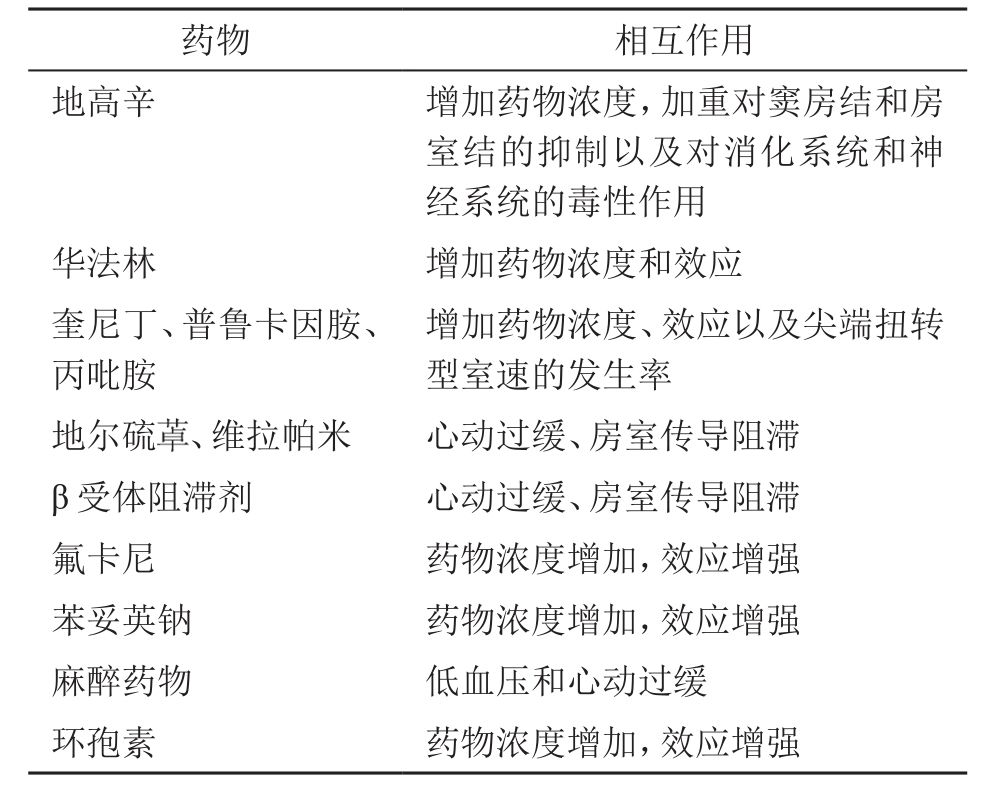
\includegraphics[width=3.29167in,height=2.61458in]{./images/Image00578.jpg}

\paragraph{转诊给专科医生}

在心律失常得以稳定控制之前,可能需要专科医生进行监护和电生理检查、行消融治疗、置入ICD或起搏器、进行程控等。如果经治医生掌握胺碘酮的用量、副作用和随访的专门知识,并不一定需要心律失常专科医生随访。随访中将患者转诊给心律失常专科医生的主要的指征是心律失常恶化,其次是出现胺碘酮的毒性作用、需要调整剂量或停药。

\subsection{结语}

胺碘酮是目前应用最广泛的一个抗心律失常药物,它是以Ⅲ类作用为主的多通道阻滞剂,能终止各种室上性和室性快速心律失常,无论对自律性增加、触发活性或折返激动都有效。因其促心律失常作用小、不影响室内传导、无负性肌力反应、不增加起搏阈值、有良好的抗颤作用,所以主要用于各种器质性心脏病、急性冠状动脉综合征、心肌肥厚、左室功能不全、室内传导阻滞中抗快速心律失常。胺碘酮可作为有症状性房颤伴左室功能不全或慢性心衰的一线治疗,可用于导致心脏骤停的恶性心律失常及血流动力学稳定的室速,此外也可作为ICD的辅助用药,减少放电次数。心脏外科围术期可预防性应用胺碘酮。胺碘酮合用β受体阻滞剂可有效控制电风暴。

胺碘酮是呋喃类结构含碘化合物,因此慢性应用可诱发甲减或甲亢,也能引起肺纤维化等心外副作用,因此应严格掌握适应证,并在应用中加强随访。急性静脉应用中可出现低血压、心动过缓、静脉炎,因此需有心电和血压监护,并选用大静脉滴注。

胺碘酮治疗反应个体差异甚大。本指南的编写根据国内外有关临床应用指南、循证资料、临床报告和荟萃分析,提出了在不同心律失常中应如何使用胺碘酮。在临床实践中提倡既有证可循,又个体化地治疗患者。

\protect\hypertarget{text00426.html}{}{}

\chapter{利 尿 药}

利尿药是一类促进体内电解质(Na\textsuperscript{+}
为主)和水分的排出而增加尿量的药物,通过影响肾小球的滤过、肾小管的重吸收和分泌等功能而实现其利尿作用,但主要是影响肾小管的重吸收。

正常人每日排尿(终尿)约1~2L,但每日的肾小球滤过液(原尿)可达180L左右,原尿流经肾小管全长形成终尿时,99\%的水分被重吸收,这是由于肾小管对Na\textsuperscript{+}
重吸收的结果。虽然近曲小管对Na\textsuperscript{+}
的重吸收率最高(65\%~70\%),但仅抑制此处的药物并不呈现明显的利尿作用,这是因为随小管液容量的增加,流速变慢,小管液与小管上皮细胞的接触面增加和接触时间延长,代偿性增加了肾小管各部(包括近曲小管本身)对Na\textsuperscript{+}
和水的重吸收率。目前临床最强的利尿药主要是抑制髓袢升支髓质部对Na\textsuperscript{+}
的重吸收,这是由于该部在主动重吸收Cl\textsuperscript{−}
和重吸收Na\textsuperscript{+}
的同时,水分却不易被动重吸收(即尿的稀释功能),Cl\textsuperscript{−}
和Na\textsuperscript{+}
在此处的重吸收率是肾髓质高渗状态的决定因素,这种高渗状态在抗利尿激素(ADH)的存在下又促进集合管对水分的大量重吸收(即尿的浓缩功能)。由此可见,肾髓质渗透压越高,尿的浓缩功能越强;反之,当药物抑制髓袢升支髓质部的尿和稀释功能而使肾髓质渗透压降低时,尿的浓缩功能减弱,从而产生强的利尿作用。Na\textsuperscript{+}
主动重吸收还包括遍及肾小管全长的Na\textsuperscript{+}
-H\textsuperscript{+} 交换,以及远曲小管和集合管的Na\textsuperscript{+}
与K\textsuperscript{+} 的交换。H\textsuperscript{+} 由H\textsubscript{2}
CO\textsubscript{3} 解离而得:H\textsubscript{2} CO\textsubscript{3}
↔H\textsuperscript{+} +{} ,而H\textsubscript{2} CO\textsubscript{3}
在肾小管上皮细胞内的形成有赖于碳酸酐酶的活性,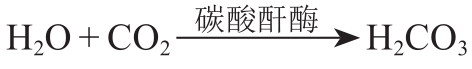
\includegraphics[width=1.5625in,height=0.21875in]{./images/Image00580.jpg}
;K\textsuperscript{+}
的分泌为醛固酮所促进。故凡能抑制碳酸酐酶或对抗醛固酮的药物均有较弱的利尿作用。

利尿药主要应用于治疗水肿性疾病,与降压药合用治疗高血压,在某些能经肾脏排泄的药物、毒物中毒时,本类药物能促使这些物质的排泄。常用的利尿药主要根据其作用部位、化学结构及作用机制分为以下4类:①主要作用于髓袢升支髓质部的利尿药(袢利尿药):呋塞米、依他尼酸、布美他尼、吡咯他尼、阿佐塞米、托拉塞米、汞撒利等,为强(高)效利尿药。依他尼酸有较强的耳源性毒性,目前已很少用。②主要作用于髓袢升支皮质部的利尿药:噻嗪类、氯噻酮等,为中效利尿药。③主要作用于远曲小管的利尿药;螺内酯、氨苯蝶啶、阿米洛利等,为潴钾利尿药。④主要作用于近曲小管的利尿药:乙酰唑胺等碳酸酐酶抑制剂。后两类均为弱利尿药。

临床常用的利尿药有:

\subsubsection{呋塞米(呋喃苯胺酸,furosemide,速尿,利尿灵,}
frusemide,fursemide)

\paragraph{药理与应用}

本品为高效利尿药。主要抑制髓袢升支髓质部和皮质部对Cl\textsuperscript{−}
和Na\textsuperscript{+}
的重吸收,该段存在着一种同时转运1个Na\textsuperscript{+}
、1个K\textsuperscript{+} 和2个Cl\textsuperscript{−}
的同向转运体系,且可双向进行。呋塞米等药物与该体系呈可逆性结合,并与氯化物竞争细胞膜上的氯化物结合位置而降低该体系的转运能力,从而影响肾髓质高渗状态的形成和维持,减弱尿的浓缩功能,促进Cl\textsuperscript{−}
、Na\textsuperscript{+} 、K\textsuperscript{+}
和水分的大量排出,显示强大的利尿效应。此外,本药还扩张肾血管,通过肾素血管紧张素(RA)系及前列腺素(PG)系作用使肾血流量增加,髓质血流量增加及不相称的渗透压降低,故有促进利尿作用。与噻嗪类利尿药不同的是Ca\textsuperscript{2+}
排出亦增多,不引起高血钙。由于尿中Cl\textsuperscript{−}
、Na\textsuperscript{+} 、K\textsuperscript{+} 和H\textsuperscript{+}
排出增加,而{}
的排出不增加,故长期反复用药可出现低盐综合征、低氯血症性和低钾血症性碱血症。口服后20~30分钟内开始利尿,1~2小时达最高峰,持续6~8小时;肌肉注射达峰时间30分钟左右,作用维持4~6小时;静注后2~5分钟出现作用,0.5~1.0小时发挥最大效应,持续2~4小时。临床上用于治疗心脏性水肿、肾性水肿、肝硬化腹水、功能障碍或血管障碍所引起的周围性水肿,并可促使上部尿道结石的排出。其利尿作用迅速、强大,多用于其他利尿药无效的严重病例。由于水、电解质丢失明显等原因,故不宜常规使用。静脉给药可治疗急性肺水肿和脑水肿。药物中毒时可用以加速毒物的排泄。

\paragraph{用法}

①肌注或静注:剂量视病情需要而定,一般20~160mg/次,静注必须缓慢,不宜与其他药物混合注射。②口服:开始时40mg/d,以后根据需要可增至80~120mg/d。分2~3次服用。儿童口服量开始按1~2mg/kg,再视情况酌增。长期(7~10天)用药后利尿作用消失,故需长期应用者,宜采取间歇疗法,给药1~3天,停药2~4天。

\paragraph{制剂}

注射液:每支20mg(2ml);片剂:每片20mg。

\paragraph{注意事项}

本品毒性低,可能出现轻微恶心、腹泻、药疹、瘙痒、视力模糊等副作用,有时可发生起立性眩晕、乏力、疲倦、肌肉痉挛、口渴,少数病例有白细胞减少,个别病例出现血小板减少、多形性红斑、直立性低血压。长期和大量应用可发生低血钠、低血钾、低血氯、低血镁、高尿酸血症、血糖升高、碱血症;水肿伴循环血量减少时,大剂量过度利尿有形成血栓、循环功能不全或肾功能恶化的危险。本品还可致暂时性耳聋或听力减退,可抑制氨基糖苷类抗生素的排出,应避免同时使用。本品若与苯妥英钠合用,可降低本品的利尿效应达50\%。对低钾血症、超量服用洋地黄、肝昏迷患者禁用,晚期肝硬化患者慎用。

\subsubsection{布美他尼(丁尿胺,bumetanide,丁苯氧酸)}

\paragraph{药理与应用}

本品为髓袢利尿药,其作用部位、作用机制、电解质丢失和作用特点均与呋塞米相似。具有高效、速效、短效和低毒的特点。其最大利尿效应与呋塞米相同,但所需剂量仅为呋塞米的1/40。口服后30分钟起效,1~2小时达高峰,作用持续3~6小时;静注后约5分钟开始利尿,0.5~1小时达高峰,作用持续2~3小时。对近曲小管也有明显作用,还可有扩张肾血管作用。由于其抑制碳酸酐酶的作用较弱,因而其钾丢失较呋塞米轻。本品口服吸收迅速且完全,生物利用度约80\%,血浆蛋白结合率为95\%;主要经肾以原形排泄,肾小管分泌在药物消除中占重要地位,24小时内可排出服用剂量的65\%。肾功能衰竭时仍能从循环中迅速移出。临床上主要作为呋塞米的代用品,用于各种顽固性水肿及急性肺水肿。对急慢性肾功能衰竭患者尤为适宜,因为本品除具有呋塞米促进肾血流量和肾小球滤过率外,还由于本品在尿液中所需的摩尔浓度较呋塞米低得多,故肾功能衰竭时,本品的利尿作用的减弱程度远低于呋塞米。在某些肾衰患者用大剂量呋塞米无效时,布美他尼可能有效。

\paragraph{用法}

口服:每次0.5~1mg,每日1~3次。静注:每次0.5~1mg,或依病情而定。

\paragraph{制剂}

片剂:每片1mg;注射液:每支0.5mg(2ml)。

\paragraph{注意事项}

①本品副作用同呋塞米,如引起低盐综合征、低氯血症、低钾血症、高尿酸血症和高血糖等。但低钾血症的发生率较呋塞米、噻嗪类利尿药为低。长期或大量应用时应定期检查电解质。②强大的利尿作用引起低血容量而增加近曲小管对Ca\textsuperscript{2+}
的重吸收,可使血钙升高,如同时补充排出的Na\textsuperscript{+}
,并使每小时尿量达到500~1000ml,可使每小时80mg的Ca\textsuperscript{2+}
排出,4~8小时后血清Ca\textsuperscript{2+}
浓度下降3\%。③肾功能不全患者使用大剂量时可能发生皮肤、黏膜及肌痛,大多数持续1~3小时后可自行消失;如疼痛剧烈或持续较久,应停药。④少数患者可有短暂的粒细胞降低、血小板减少,偶有恶心、呕吐、男子乳房发育、皮疹等。

\subsubsection{托拉塞米(torasemide,托拉沙得,伊迈格)}

\paragraph{药理与应用}

本品为一种较新的髓袢利尿药,其作用特点有:①10~20mg本品与40mg呋塞米的排钠作用相当。其排钾作用明显弱于其他髓袢利尿药,这在治疗伴有低钾血症的心衰等疾病时具有特殊重要的临床意义。髓袢利尿药的利尿强度排序大致为:布美他尼>托拉塞米>吡咯他尼>呋塞米。②扩张血管作用:由于肾脏血管扩张、肾血流阻力降低,因而肾皮质深部的血流量增加,可在一定程度上预防急性肾衰竭,保护残余肾功能。③生物半衰期较呋塞米长,通常每日只需用药一次,几乎无利尿抵抗现象。口服生物利用度(80\%~90\%)高于呋塞米(40\%~50\%),口服与非肠道用药的疗效几乎一样。④在相当大的治疗剂量范围内,具有非常良好的量效关系,连续用药无蓄积,安全性远远高于其他髓袢利尿药。依适应证的不同,剂量调整范围可以从用于降压的2.5mg到用于严重肾衰竭的200mg。⑤通过增加尿量,减少机体水钠潴留,降低心脏前负荷,还可扩张肺血容量而降低心脏后负荷,并有降低肺毛细血管通透性、抑制肺水肿形成和发展的作用。⑥对血清镁、尿酸、糖和脂质类无明显影响。口服后吸收迅速。临床用于:①各种原因的水肿,如充血性心力衰竭、急性肺水肿、肾性水肿、肝硬化腹水、肝癌腹水、脑水肿及其他水肿等;②急、慢性心力衰竭;③高血压病;④急、慢性肾衰竭;⑤急性中毒。

\paragraph{用法}

口服或静脉注射:初始剂量每次5~10mg,每日1次。依适应证不同最高可用至100~200mg/d。

\paragraph{制剂}

片剂:每片2.5mg;5mg;10mg;20mg;注射液:每支10mg(1ml);20mg(2ml)。

\paragraph{注意事项}

①禁用于肾衰竭无尿、肝性脑病、低血压休克、尿道梗阻所致严重排尿困难,以及对本品过敏者。②不良反应类似呋塞米。

\subsubsection{氢氯噻嗪(hydrochlorothiazide,双氢克尿噻,双氢氯噻嗪,esidrex)}

\paragraph{药理与应用}

本品为噻嗪类利尿药。主要抑制髓袢升支皮质部对Na\textsuperscript{+}
和Cl\textsuperscript{−}
的再吸收,从而促进肾脏对氯化钠的排泄而产生利尿作用,为一中效利尿药。还具有微弱的抑制碳酸酐酶的作用,故尿中HCO\textsubscript{3}
\textsuperscript{−} 丢失较轻。本品还增加Mg\textsuperscript{2+}
的排泄,减少钙及尿酸的排泄,并降低肾小球的滤过率。口服后1小时出现作用,约2小时达高峰,维持12~18小时。本品还有降压作用,并能增强其他降压药的降压作用,临床上作为基础降压药与其他降压药合用。还有抗利尿作用,减少尿崩症患者的尿量,但疗效不及脑垂体后叶素,作用机制不详。本品在临床上主要用于各种水肿(心脏性水肿效果较好)、各期高血压及尿崩症。

\paragraph{用法}

①治疗水肿:25~75mg/d,需要时可增至100mg/d,两次分服。间日或每周1~2次服用。至恢复原体重后,可减至维持量。②治疗心脏性水肿:开始时用小剂量,12.5~25mg/d,以免因盐及水分排泄过快而引起循环障碍或其他症状。③治疗肝硬化腹水:最好与螺内酯合用。④治疗高血压:多与其他降压药合用。开始时50~75mg/d,1周后减为25~50mg/d的维持量。

\paragraph{制剂}

片剂:每片10mg;25mg;50mg。

\paragraph{注意事项}

①服用期间,应定期检查血液电解质。长期服用可致低钠血症、低氯血症和低钾血症性碱血症,宜用隔日或服药3~4天停药3~4天的间歇疗法,同时不应过分限制食盐的摄入量,多食用含钾食物或钾盐,以防血钾过低。②停药时应逐渐减量,突然停药可能引起钠、氯及水的潴留。③少数患者服药后可产生胃肠道症状,如恶心、呕吐、腹泻、气胀,以及皮肤症状如皮疹、瘙痒症、光敏性皮炎等。少数有血小板减少、粒细胞减少。部分患者发生高尿酸血症、高血糖、高血脂和高钙血症。④肝肾功能减退者和痛风、糖尿病患者慎用。

噻嗪类利尿剂除氢氯噻嗪外,还有甲氯噻嗪(methyclothiazide)、泊利噻嗪(polythiazide)、环戊噻嗪(cyclopenthiazide)、苄氟噻嗪(bendroflumethiazide)、三氯噻嗪(trichlormethiazide)、氢氟噻嗪(hydroflumethiazide)、苄噻嗪(苯噻嗪,benzthiazide)等,它们的作用特点与用法参见表\ref{tab152-1};其有关注意事项同氢氯噻嗪。

\subsubsection{螺内酯(spironolactone,安体舒通,antisterone,螺旋内酯固醇)}

\paragraph{药理与应用}

本品为醛固酮拮抗剂。与醛固酮有类似的化学结构,二者在远曲小管和集合管的皮质段部位起竞争作用,是在细胞质膜的盐皮质激素受体的水平上发生直接的拮抗作用,从而干扰醛固酮对上述部位钠重吸收的促进作用,促进Na\textsuperscript{+}
和Cl\textsuperscript{−} 的排出而产生利尿,因Na\textsuperscript{+}
-K\textsuperscript{+}
交换机制受抑,钾的排出减少,故为潴钾利尿药。本品利尿作用较弱,且缓慢而持久,口服后24小时左右起效,2~3天始呈现最大利尿效果,停药后仍可持续2~3天。临床上用于治疗与醛固酮升高有关的顽固性水肿,故对肝硬化和肾病综合征的患者较有效。也可用于特发性水肿的治疗。单用本品时利尿作用往往较差,常与噻嗪类、髓袢利尿药合用,既可增强疗效,又可防止低血钾。近年来已被推荐作为治疗心力衰竭的基本用药。

\paragraph{用法}

开始40~120mg/d,分3~4次口服。用药5天后如疗效满意,继续用原量,否则可加用其他利尿药。

\paragraph{制剂}

片(胶囊)剂:每片(胶囊)20mg(微粒),微粒20mg与普通制剂100mg的疗效相仿。螺内酯-噻嗪片:每片含螺内酯25mg、氢氯噻嗪25mg,1次1片,每天1~4次。

\paragraph{注意事项}

①服后可能引起头痛、嗜睡、精神紊乱、运动失调、皮疹及乳腺分泌过多等,并可引起低钠血症、高钾血症。②与噻嗪类利尿剂合用,可取长补短,合用后疗效增加,不良反应减轻。③肾功能衰竭患者及血钾偏高者忌用。

\subsubsection{氨苯蝶啶(triamterene,三氨蝶啶)}

\paragraph{药理与应用}

作用部位与螺内酯相同,直接抑制远曲小管和集合管皮质段对Na\textsuperscript{+}
的重吸收,增加Na\textsuperscript{+} 、Cl\textsuperscript{−}
排泄而利尿,对K\textsuperscript{+}
则有潴留作用,其潴钾排钠作用与螺内酯相似,但本品不是醛固酮拮抗剂。与其他利尿药如噻嗪类或螺内酯合用时,能显著增强各自的利尿作用和减轻不良反应。本品利尿作用较弱,但尚迅速,服后2小时即产生利尿作用,4~6小时作用达高峰,药效可持续12~16小时。本品在肝脏内代谢,原形和代谢物主要由肾脏排泄。临床上用于治疗心力衰竭、肝硬化和慢性肾炎等引起的顽固性水肿或腹水,以及糖皮质激素治疗过程中发生的水钠潴留。常与排钾利尿药合用。亦用于对氢氯噻嗪或螺内酯无效的病例。

\paragraph{用法}

每日2次,每次25~50mg,饭后服,最大剂量每日不宜超过300mg。与氢氯噻嗪合用疗效更显著,两者均应减量。

\paragraph{制剂}

片剂:每片50mg(黄色)。氨苯蝶啶-氢氯噻嗪片(Diazide):每片含氨苯蝶啶50mg,氢氯噻嗪25mg,每次1片,每日1~4次。

\paragraph{注意事项}

①服后偶出现恶心、呕吐、嗜睡、轻度腹泻、软弱、口干及皮疹等。②大剂量长期使用或与螺内酯合用,可致高血钾,停药后可逐渐消失。③孕妇及育龄的已婚妇女慎用,应随时注意血象变化、肝功能或其他特异反应。④严重肝、肾功能不全者、有高血钾倾向者忌用。

\subsubsection{阿米洛利(氨氯吡咪,amiloride,amipromizide)}

\paragraph{药理与应用}

本品作用部位及作用机制与氨苯蝶啶相似,在远曲小管及集合管皮质段抑制Na\textsuperscript{+}
-H\textsuperscript{+} 和Na\textsuperscript{+} -K\textsuperscript{+}
交换,亦非通过拮抗醛固酮而起作用,为目前排钠潴钾利尿药中作用最强的药物。口服后2小时起效,6~8小时作用达高峰,可持续24~48小时。本品增加Na\textsuperscript{+}
、Cl\textsuperscript{−}
的排泄和尿酸的排泄。一般不单独应用。本品能增强氢氯噻嗪和依他尼酸等利尿药的作用并减少钾的丢失。

\paragraph{用法}

开始2.5~5mg,一日1次;必要时可增加剂量,但每日不宜超过20mg。

\paragraph{制剂}

片剂:每片2.5mg;5mg。复方盐酸阿米洛利片(武都力,Moduretic):每片含阿米洛利2.5mg、氢氯噻嗪25mg,每日1~2次,每次1~2片。复方呋塞米片(福洛必,FLB):每片含阿米洛利2.5mg,呋塞米20mg,每日1次,每次1片。

\begin{table}[htbp]
\centering
\caption{其他噻嗪类利尿药}
\label{tab152-1}
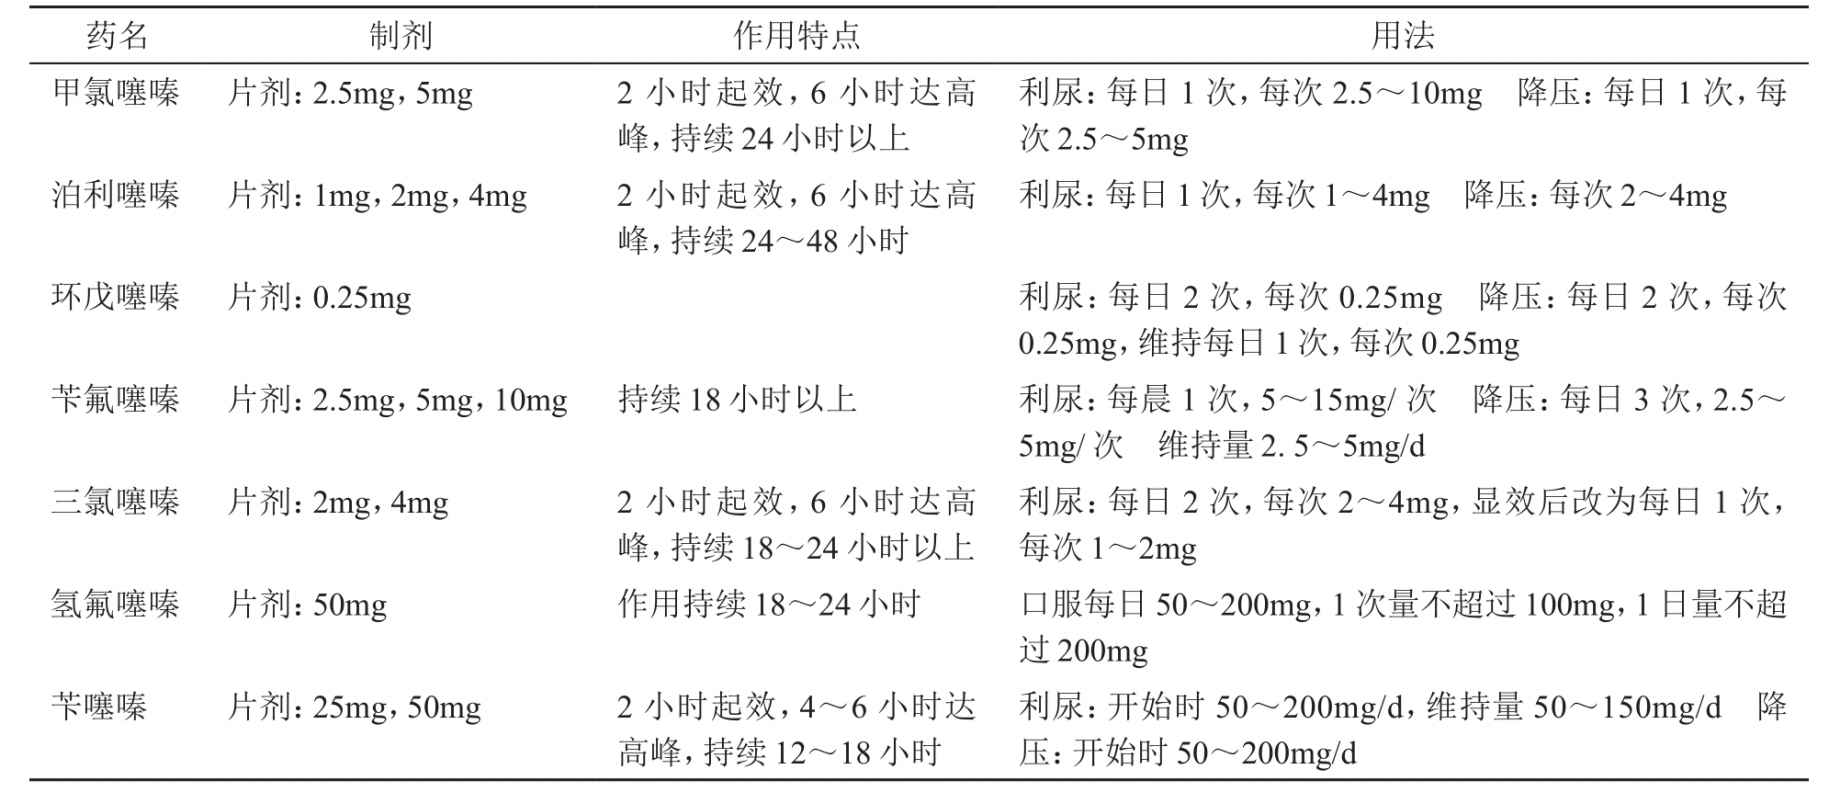
\includegraphics[width=6.625in,height=2.86458in]{./images/Image00582.jpg}
\end{table}

\paragraph{注意事项}

与氨苯蝶啶相同。

\subsubsection{乙酰唑胺(acetazolamide,醋唑磺胺,醋氮酰胺, diamox)}

\paragraph{药理与应用}

本品为碳酸酐酶抑制剂。肾小管上皮细胞、胃黏膜、胰腺细胞、眼睫状体上皮细胞、红细胞和中枢神经细胞均有碳酸酐酶分布,当该酶活性受抑时,各种需大量及连续供应H\textsuperscript{+}
及HCO\textsubscript{3} \textsuperscript{−}
的功能均受影响。本品在近曲小管非竞争性抑制碳酸酐酶,以致碳酸在肾小管上皮细胞内离解为H\textsuperscript{+}
及HCO\textsubscript{3} \textsuperscript{−}
被抑制,伴随肾小管H\textsuperscript{+} 的分泌及HCO\textsubscript{3}
\textsuperscript{−} 再吸收减少,Na\textsuperscript{+}
的再吸收减少,携水排出而利尿,其结果尿中HCO\textsubscript{3}
\textsuperscript{−} 、Na\textsuperscript{+} 、K\textsuperscript{+}
、水排出均增加。细胞外液中HCO\textsubscript{3} \textsuperscript{−}
降低,趋向代谢性酸中毒,但血中HCO\textsubscript{3} \textsuperscript{−}
减低时,本品抑制HCO\textsubscript{3} \textsuperscript{−}
再吸收的作用亦减弱,致利尿作用亦减弱,故本品利尿作用较弱。本品抑制眼内结构中的碳酸酐酶,可降低房水生成速度,还可降低由脉络丛产生脑脊液的速率,故可用于治疗青光眼和脑水肿。口服后30分钟产生作用,2~4小时达作用高峰,持续12小时。临床上治疗心脏性水肿可提高强效利尿药效果:顽固性心衰患者对强效利尿药产生抵抗时,用本药抑制近曲小管的钠、水回吸收,从而增加髓袢的负荷量,可以提高利尿效果。但对肾性及肝性水肿无效。尚可作为控制癫痫小发作的辅助药。

\paragraph{用法}

①治疗心脏性水肿:每日1次,每次0.25~0.5g,早餐后服用。②治疗青光眼和脑水肿:每日2~3次,每次0.25g。青光眼急性发作时的抢救或某些恶心、呕吐不能口服的患者,可静脉或肌内注射本品。③癫痫小发作:每日1次,每次0.5~1.0g。与其他药物合用时则不超过0.25g。

\paragraph{制剂}

片剂:每片0.25g。注射用乙酰唑胺:0.5g/支。

\paragraph{注意事项}

①常见不良反应有困倦、面部和四肢麻木感。严重不良反应为粒细胞缺乏症(系过敏反应),以及由于代谢性酸血症降低尿中枸橼酸盐的排出和碳酸钙沉淀所致的尿结石,故有尿结石病史者不宜应用。②可引起肾脏并发症,如肾绞痛、结石症、磺胺尿结晶、肾病综合征等。为预防其发生,除按磺胺类药物预防原则外,尚须加服钾盐、镁盐等。③应避免应用钙、碘及广谱抗生素等可增加碳酸酐酶活性的药物。④肝昏迷、肾功能及肾上腺皮质功能严重减退、代谢性酸血症以及伴有低钾血症的水肿患者不宜用,亦不宜用于肺心病、心力衰竭患者。⑤本品主要用于治疗青光眼,少作利尿药应用。

\protect\hypertarget{text00427.html}{}{}

\hypertarget{text00427.htmlux5cux23CHP17-5-9}{}
参 考 文 献

1.
陈新谦,金有豫,汤光.新编药物学.第17版.北京:人民卫生出版社,2011:566

2. 杨宝峰 .药理学.第6版.北京:人民卫生出版社,2004:232

\protect\hypertarget{text00428.html}{}{}

\chapter{肾上腺皮质激素}

肾上腺皮质激素(adrenocortical
hormones)是肾上腺皮质所分泌的激素的总称,属甾体类化合物。按其生理作用可分为三类:①盐皮质激素(mineralocorticoids),由肾上腺皮质球状带分泌,以醛固酮(aldosterone)为代表,主要影响水盐代谢。②糖皮质激素(glucocorticoids,GC),由肾上腺皮质束状带合成和分泌,以氢化可的松(hydrocortisone)为代表,主要影响糖和蛋白质代谢。③性激素(sex
hormones),由肾上腺皮质网状带所分泌,以脱氢异雄酮为代表,因其促进蛋白质合成作用,故也称之氮皮质激素。临床常用的皮质激素是指糖皮质激素,它具有多方面药物作用,应用十分广泛。现就糖皮质激素(以下简称“激素”)的药理作用、临床应用,尤其在急危重症中的运用以及有关事项简介如下。

\subsubsection{药理作用}

\hypertarget{text00428.htmlux5cux23CHP17-6-1-1}{}
(一) 抗炎作用

激素具有强大的抗炎作用
,能抑制感染性和非感染性(如过敏性、机械性、化学性等)炎症。在炎症早期可减轻渗出、水肿、毛细血管扩张、白细胞浸润及吞噬反应,从而改善红、肿、热、痛等症状;在后期可抑制毛细血管和成纤维细胞的增生,延缓肉芽组织生成,防止粘连及瘢痕形成,减轻后遗症。抗炎作用的机制为:①直接作用于血管或加强血管平滑肌对儿茶酚胺的敏感性,收缩血管和降低通透性,减少渗出;②可抑制炎症组织合成与释放组胺、5-羟色胺(5-HT)、激肽、前列腺素等介质;③稳定生物膜,包括细胞膜和细胞器膜,尤其是溶酶体膜,可防止因有害刺激(如细菌内毒素、低氧、酸中毒等)而释出多种溶酶体水解酶;④通过激素对血管的作用,以及减少炎症介质的形成或释放,使白细胞的趋化作用减弱,减少炎症细胞的侵入。应注意,炎症反应是机体的一种防御功能,炎症后期的反应更是组织修复的重要过程,因此,激素在抑制炎症、减轻症状的同时,也降低机体的防御功能,可致感染扩散,阻碍创口愈合。

\hypertarget{text00428.htmlux5cux23CHP17-6-1-2}{}
(二) 抗毒素作用

激素可提高机体对有害物质刺激的耐受性
,有显著保护机体免受细菌内毒素的毒害作用。但激素不能中和内毒素,也不能保护机体免受细菌外毒素的损害。激素在感染性毒血症中的解热和改善中毒症状的作用,与它能稳定溶酶体膜有关,也因它能减少内热原的释放并降低体温调节中枢对热原的敏感性。

\hypertarget{text00428.htmlux5cux23CHP17-6-1-3}{}
(三) 抑制免疫和抗过敏作用

由于炎症
、免疫、过敏三者关系密切,涉及共同的细胞反应和体液介质。激素对上述过程的许多环节均有抑制作用:①抑制抗原-抗体反应引起肥大细胞脱颗粒而释放组胺、5-HT等介质的产生,从而减轻一系列过敏反应症状;②激素能抑制人淋巴细胞DNA和蛋白质合成,干扰淋巴组织在抗原作用下的分裂和增殖,并能阻断致敏T淋巴细胞释放的各种淋巴因子(如白细胞趋化因子等)和抑制单核-巨噬细胞系统对抗体包埋细胞的清除;③激素能使体内淋巴细胞发生重新分配,血液循环中淋巴细胞(主要是T淋巴细胞)和单核细胞总数显著减少(与骨髓释出延迟有关),故在免疫活性细胞的数量上减轻了免疫反应。

\hypertarget{text00428.htmlux5cux23CHP17-6-1-4}{}
(四) 抗休克作用

大剂量激素已广泛用于各种严重休克,尤其是中毒性休克的治疗。其机制为:①改善血管对血管活性药物的反应性,解除血管痉挛,改善微循环;②通过稳定溶酶体膜的作用,减少心肌抑制因子(myocardio-depressant
factor,MDF)的形成,从而防止蛋白水解酶的释放以及由MDF引起的心肌收缩减弱,防止心输出量降低和内脏血管收缩等循环障碍;③增强血红蛋白氧合能力,促进组织内氧的释放;并增强线粒体氧化磷酸化功能,增加cAMP含量,从而改善组织新陈代谢,对抗内毒素以及体内有害代谢产物对细胞的损害。

\subsubsection{适应证与禁忌证}

\hypertarget{text00428.htmlux5cux23CHP17-6-2-1}{}
(一) 适应证

常见的适应证有:①急、慢性肾上腺皮质功能不全(包括肾上腺危象)、脑垂体前叶功能减退及次全切除术后作替代疗法;②严重感染并发的毒血症,如中毒性菌痢、中毒性肺炎、暴发型流脑等;③自身免疫性疾病,如风湿热、风湿性心肌炎、风湿性及类风湿关节炎、SLE、结节性动脉炎、皮肌炎、自身免疫性溶血性贫血和肾病综合征等;④器官移植的急性排斥反应;⑤过敏性疾病,如荨麻疹、血清病、血管神经性水肿、过敏性鼻炎、支气管哮喘、过敏性休克等;⑥缓解急性炎症的各种症状,并可阻止某些炎症的后遗症,如组织粘连、瘢痕。可用于结核性脑膜炎、胸膜炎、心包炎、虹膜炎、角膜炎、视网膜炎、视神经炎、睾丸炎和烧伤等;⑦各种原因引起的休克;⑧血液系统疾病,如白血病、恶性淋巴瘤、再生障碍性贫血、原发性血小板减少性紫癜等;⑨其他肌肉和关节劳损、严重天疱疮、剥脱性皮炎、溃疡性结肠炎等。

\hypertarget{text00428.htmlux5cux23CHP17-6-2-2}{}
(二) 禁忌证

常见的禁忌证有
:①对激素过敏者;②活动性消化性溃疡;③新近胃肠吻合术后;④严重骨质疏松或骨折未愈合前;⑤严重的糖尿病;⑥严重的低钾血症;⑦未能用抗感染药物控制的细菌、真菌等感染性疾病;⑧肾上腺皮质功能亢进症(患者在接受垂体或肾上腺手术治疗时及手术后例外);⑨严重高血压(系统性红斑狼疮引起狼疮危象等例外);⑩妊娠初期(14周内服用大量激素有引起胎儿发生先天性缺陷,如兔唇、腭裂以及早产、流产的危险)和产褥期;{}
水痘、牛痘接种、单纯疱疹角膜炎;{} 有严重的精神病史或癫痫病史;{}
青光眼或角膜溃疡。

当适应证与禁忌证同时并存时,应全面分析,权衡利弊,慎重决定。遇有危及生命的紧急情况确需用激素者,即使存在禁忌证,也可短期使用之,一旦危情度过,即应尽早停药或减量。

\subsubsection{激素的剂型}

口服、注射均可吸收。用于口服的剂型有氢化可的松(hydrocortisone,皮质醇)、可的松(cortisone,皮质素)、泼尼松(强的松,prednisone,去氢可的松)、泼尼松龙(强的松,prednisolone,氢化泼尼松)、地塞米松(氟美松,dexamethasone)、甲泼尼龙(甲基强的松龙,methylprednisolone)等;氢化可的松琥珀酸钠、泼尼松龙琥珀酸钠、地塞米松水剂、甲泼尼龙琥珀酸钠注射液等可供静脉注射或滴注用,可在注射后立即发生效应,适用于病情危重者。

可的松和泼尼松经口服后在肝内分别转化为氢化可的松和泼尼松龙而生效,故严重肝功能不全的患者只宜用氢化可的松或泼尼松龙;但实际上因肝功能不良而影响可的松和泼尼松转化的情况极为少见。与肝微粒体酶诱导剂如苯巴比妥、苯妥英钠等合用时需加大皮质激素的用量。

口服片剂服用后在血浆中的半衰期长短各异,但不论何种制剂口服12小时后虽在血浆中完全消失,但其与细胞内受体结合所产生的生物效应,则可持续相当时间。根据其血浆半衰期和生物效应时间的长短,可将激素分为短、中和长效三类,它们之间的比较见表\ref{tab153-1}。

促皮质素(促肾上腺皮质激素,adrenocorticotropic
hormone,ACTH)系通过刺激肾上腺皮质分泌皮质醇等类固醇激素而发挥其药理作用。故临床用途与皮质激素基本相同。在极少数情况下用激素疗效不佳时,改用ACTH后有较好疗效。但对肾上腺皮质已萎缩、肾上腺皮质功能完全丧失的患者无效,须改用皮质激素。注射ACTH后,皮质醇分泌量取决于肾上腺皮质的反应性、药物剂型与剂量以及给药途径与持续时间。为获得最大的肾上腺皮质激素分泌量效应,可选用ACTH静脉或肌内注射。临床上以静脉注射为常用,方法为ACTH
12.5~25U置入500ml液体中静滴6~8小时。ACTH
12.5~25U肌注,每日2次;或ACTH长效制剂20~60U,每日肌注1次,可获相同效果。临床常用的ACTH系从家畜脑垂体前叶提取,其抗原性不同于人类ACTH,注射后可引起过敏反应,应予注意。

\subsubsection{激素的使用方法}

\hypertarget{text00428.htmlux5cux23CHP17-6-4-1}{}
(一) 替代治疗

适用于原发或继发性肾上腺皮质功能不全患者的长期治疗。通常选用氢化可的松或可的松(皮质素),每天前者为20~30mg,后者为25~37.5mg,总量的2/3一般在早餐后给,余1/3下午给。发生肾上腺危象时,一般采用氢化可的松静注,开始24小时用量为300~500mg,病情好转后减量并改口服给药,病情稳定后继续维持量治疗。

\hypertarget{text00428.htmlux5cux23CHP17-6-4-2}{}
(二) 非替代治疗

即发挥激素的抗炎
、抗过敏、抗休克和免疫抑制作用的用药方法。所用激素的剂量和疗程需根据病情的特殊性以及预期的激素疗程和可能出现的危害个别拟定。对某些急危重症和变态反应性疾病等,一般采用短程疗法(几天)或中程疗法(几周或几个月);而某些对激素有效的疾病,如肾病综合征、系统性红斑狼疮等则常常需长期疗法(几年至数十年)。由于激素的非替代治疗属于非特异性治疗范畴,并不针对病因,不能改变疾病本身的自然过程,故激素剂量宜调整到最小有效剂量,并采取隔日或间歇疗法,以保存患者自身HPA轴的完整性,从而减轻对外源激素的依赖程度。激素作为非替代治疗应用的药物与一般药物不同,利弊全在于掌握的得失。评价激素治疗价值应权衡疗效(病情得以控制的程度)及其潜在的危险。一次或数天内(如3~5天)应用大量激素,一般是较安全的;若连续用药时间超过2~3周,即使用量不很大,也会出现HPA轴的抑制以及过量反应。在激素使用期间,若任意停药,也会出现停药反应。激素的非替代治疗有以下几种方法:

\begin{table}[htbp]
\centering
\caption{常用肾上腺皮质激素制剂的比较}
\label{tab153-1}
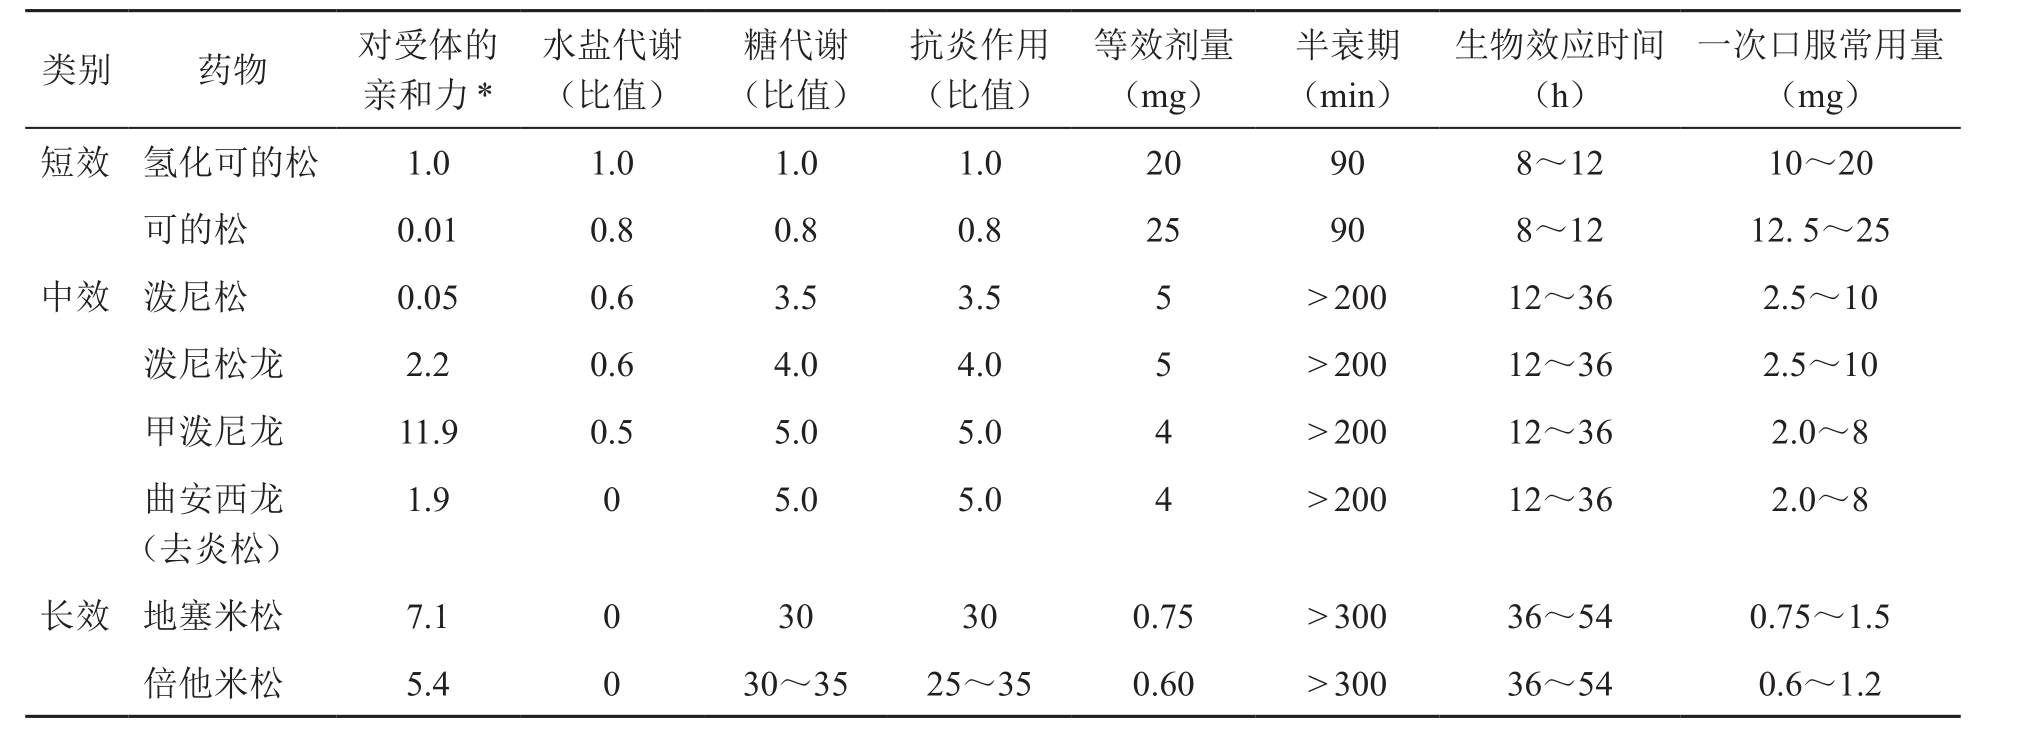
\includegraphics[width=6.73958in,height=2.42708in]{./images/Image00586.jpg}
\end{table}

\textsuperscript{*} 胎儿肺细胞

\paragraph{冲击疗法}

即大剂量短程疗法。如用琥珀酸钠甲泼尼龙(甲基强的松龙)15~30mg/kg静脉注射,每日1~2次,必要时每8~12小时1次,连续2~3天。该疗法主要用于抢救危急重症病例,如严重过敏反应、甲状腺危象、脏器移植急性排异反应、异型输血反应、急性血管神经性水肿、狼疮性脑病、狼疮性肾炎等。该疗法的优点是剂量大,因而作用强,又保持了HPA轴的完整功能,减少激素的过量反应。

\paragraph{短程疗法}

适用于毒性症状严重、机体变态反应较强者。应用激素的目的是减轻毒性症状,减轻机体的免疫反应和炎症反应,降低器官性损害的严重程度。常用于结核性胸膜炎、结核性脑膜炎(早期)等,应用激素的疗程约4~6周。

\paragraph{中程疗法}

适用于某些病程较长伴有多脏器损害的疾病,如急性风湿热等,应用激素的疗程约2~3个月。

\paragraph{长效疗程}

适用于反复发作的自身免疫性疾病,如SLE、肾病综合征、血小板减少性紫癜等,应用激素的疗程半年至一年或更长时间。

\paragraph{给药方式}

\hypertarget{text00428.htmlux5cux23CHP17-6-4-2-5-1}{}
(1) 分次给药法:

是临床上最常用的口服给药法,常分1天3次口服。每日总量视病情而定,以泼尼松为例开始用量为:病情轻、中度,20~30mg/d;中度~重度,40~80mg/d;病情危急,100~200mg/d。激素疗程长短,主要决定于疾病本身的性质以及激素治疗的目的与疗效。原则上大剂量短程疗法主要用于危急重症,一旦病情转危为安,即可停药;而中长程疗法主要用于各种亚急性或慢性疾病,如原发性血小板减少性紫癜、免疫性溶血性贫血、系统性红斑狼疮、肾病综合征等,用药时间常需几个月或持续几年或更长时间。此种超生理剂量的分次给药治疗,疗程超过2~3周,即可出现HPA轴的抑制和库欣综合征等过量反应;剂量越大,分次用药时间越长,这类副作用也越重。须密切观察病情,待病情稳定后,再改以隔日给药。分次给药时间不能超过2~3周。根据病情好转程度,逐渐减量并确定最低维持量。长期用药最低维持量应高于正常安静状态皮质醇的分泌量。以泼尼松为例,其维持量为隔日15mg左右。

\hypertarget{text00428.htmlux5cux23CHP17-6-4-2-5-2}{}
(2) 间歇给药法:

激素对HPA轴的抑制作用与其血浓度有关,但其抗炎作用在其血浓度下降甚至消失后尚可持续相当时间,即一个剂量的激素与靶细胞受体结合后所产生的生物效应(主要是抗炎与免疫抑制作用)持续时间长于此一剂量对HPA轴的抑制,此乃间歇给药的基础。该疗法仅适用于慢性疾病,如系统性红斑狼疮、肾病综合征等,经激素分次给药治疗,病情已获控制而仍须继续巩固治疗者。具体用药方法除多次短程静脉冲击疗法外,常用的是口服激素,每周服3~4天(剂量为1周总量),然后停药4天或3天,如此每周重复并调整剂量;或采用隔日疗法,它是目前最常用的间歇给药法。每隔日早晨8时前1次服下2天的总量。实验证明,HPA轴对早晨给予激素最不敏感(此时正值内源性ACTH和皮质醇分泌高峰),而对午夜前给予激素最为敏感(此时体内分泌的ACTH和皮质醇浓度最低)。临床观察也证明,原接受每天分次给药的患者,改为隔日给药后,有的不仅能维持疗效,而且由于HPA轴恢复正常或接近正常,所需维持量逐渐减少,过量反应大为减轻甚至消失,且有利于停药。

\hypertarget{text00428.htmlux5cux23CHP17-6-4-3}{}
(三) 激素撤减方法

应用激素治疗后
,若病情已获好转,或疗效不确定抑或出现严重副作用及并发症,必须减量或撤除激素。对短程冲击疗法,可立即停药,但因中、长程激素治疗后,HPA轴结构与功能的恢复需时甚长,其中ACTH分泌细胞功能的恢复约需3~6个月,一旦内源性ACTH分泌达足够水平,肾上腺皮质即可逐渐恢复其分泌功能,此过程约需9~12个月。因此,为减少或避免撤药或减量过程中的反应,需酌情选择以下撤停激素的方法:①缓慢递减剂量:以泼尼松为例,若原来维持量为20mg/d,可每周减少约2.5mg;当减至10mg/d后,可每月减少1.25mg;当减至每天维持量接近生理量后(约5mg/d),则更应放慢速度,以每月减少约0.75mg的速度减量,直至完全停用。②以每日给药过渡到隔日给药:首先将每天分次给药法改为每晨一次服药(1天总量不变),然后则从每晨一次顿服逐渐改为每2天剂量隔日晨一次顿服。隔日给药疗程长短和所需剂量多少取决于病情需要,当病情稳定无需继续激素治疗时,可直接完全撤停总剂量的激素,原则上不必递减剂量缓慢停药。

\subsubsection{激素的不良反应及其处理}

激素的不良反应实际上是激素的超生理反应,并非似一般药物所引起的副作用,其发生与给药剂量、方案、疗程长短、患者情况等因素有关。严重的不良反应和并发症可引起死亡,细菌与真菌感染是主要的死亡原因,其次是心血管并发症、消化性溃疡出血或穿孔以及胃肠吻合口穿破等。

\hypertarget{text00428.htmlux5cux23CHP17-6-5-1}{}
(一) 长期大量应用引起的不良反应

\paragraph{类肾上腺皮质功能亢进综合征(库欣综合征)}

因物质代谢和水盐代谢紊乱所致。停药后可自行消退,必要时采取对症治疗。为防止发生,可采用局部用药,尽量避免全身用药,如支气管哮喘患者,可用激素气雾吸入法,类风湿关节炎可用关节腔内注射激素制剂等,以减少对全身的影响。

\paragraph{诱发或加重感染}

因激素抑制机体防御功能所致。长期应用常可诱发感染或使体内病灶扩散,如结核病、化脓性感染和二重感染等。感染部位多为肺、泌尿道、肛周、膈下、腹腔与注射部位等。而感染症状又常被激素的抗炎作用所掩盖,如激素引起的“类固醇”溃疡并发穿孔时,患者可无全身发热和急性腹膜炎表现。因此,除了严密观察外,对感染者必要时应事先给予作用强而有效的抗菌药物。

\paragraph{消化系统并发症}

激素能使胃酸、胃蛋白酶分泌增加,抑制胃黏液分泌,降低胃肠黏膜的抵抗力,故可诱发或加重消化性溃疡,甚至造成消化道出血或穿孔;少数患者可诱发胰腺炎或脂肪肝。治疗与一般消化性溃疡及其并发症相同。可预防性应用制酸药。

\paragraph{心血管系统并发症}

长期应用可引起高血压和动脉粥样硬化。

\paragraph{精神失常}

多见于女性。早期以欣快症为最常见,从欣快感、失眠到兴奋、轻躁狂,也有表现为抑郁、焦虑,甚至有自杀倾向者。有些患者可有欣快和抑郁交替发生。也可出现妄想、幻觉、木僵等症状。其发生常与用量有关,泼尼松量大多在80mg/d以上。激素减量或停药症状常可消失。有精神病或癫痫病史者禁用或慎用。

\paragraph{其他}

①伤口愈合不良:为促进伤口愈合,饮食中应增加蛋白质,尚可加用蛋白同化激素。②肌肉萎缩:常累及臂部屈肌和肩胛肌。③骨坏死与骨质疏松:骨坏死系无菌性,常见于股骨头和股骨颈,与长期使用大量激素引起脂肪栓塞与血管炎症引起缺血有关。骨质疏松见于长期使用激素从而引起骨质吸收加速,并抑制成骨细胞活力,引起负氮和负钙平衡,影响骨质生成。骨质吸收增加(主要原因)与骨质生成减少逐渐引起骨质疏松。多见于儿童、老人和绝经妇女。④生长延迟:激素分解蛋白质的作用强,且能抑制生长激素的分泌,故儿童接受激素治疗可出现生长延迟。可采用隔日疗法或用不抑制生长激素分泌的ACTH。⑤低钾血症与类固醇糖尿病等。⑥对胎儿的影响:妊娠早期(14周前)接受大量激素,胎儿可发生兔唇、腭裂;妊娠中后期可致流产与早产。故妊娠早期应禁用,中、后期应尽量少用。

\hypertarget{text00428.htmlux5cux23CHP17-6-5-2}{}
(二) 停药反应

\paragraph{撤药综合征}

多见于大量激素治疗后突然停药或撤药速度太快,发生率约50\%~90\%。临床表现可有疲乏无力、情绪消沉、发热、恶心、呕吐、关节与肌肉痛(多发生于腓肠肌和股部肌肉、伴肌肉僵硬,以及肘、踝关节痛为主)。在出现上述症状或应激时需加用激素,待症状缓解后再缓慢减量。部分患者可出现戒断反应,表现为不安、情绪消沉、恐惧感以及周身不适等。可予心理治疗、安慰剂或适当的安定药物与抗抑郁药物。

\paragraph{反跳现象}

因患者对激素产生了依赖性或病情尚未完全控制,突然停药或减量过快而致原发病症状复发与病情加重。常需再予以激素治疗,待症状缓解后再逐渐减量、停药。

\hypertarget{text00428.htmlux5cux23CHP17-6-5-3}{}
(三) 其他

临床工作中应注意
:地塞米松注射偶可引起第Ⅰ型变态反应;ACTH生物制品系从家畜垂体提取物中制成,也可引起过敏反应。常在注射后几小时内发生荨麻疹、血管神经性水肿、发热、全身不适、气急、甚至过敏性休克。血清病样反应多在相隔几周或数月后的第二次给药时发生。艾迪生病患者对ACTH生物制剂更易发生过敏反应,须特别注意。

\protect\hypertarget{text00429.html}{}{}

\hypertarget{text00429.htmlux5cux23CHP17-6-6}{}
参 考 文 献

1.
陈新谦,金有豫,汤光.新编药物学.第17版.北京:人民卫生出版社,2011:609

2. 杨宝峰 .药理学.第6版.北京:人民卫生出版社,2004:359

3. 陈灏珠 ,林果为.实用内科学.第13版.北京:人民卫生出版社,2009:1235

\protect\hypertarget{text00430.html}{}{}

\chapter{抗 菌 药 物}

抗菌药物(包括抗生素及化学制剂)是治疗感染性疾病的特效药物,在临床救治工作中应用很多。与多数药物一样,几乎每一品种均具有一定的毒性,用得合理即为“药”,用得不适当反成“毒”,因此如何合理使用抗菌药物是每一位临床医生所必须熟悉与掌握的。

合理使用抗菌药物系指在明确指征下选用适宜的抗菌药物,并采用适当的剂量和疗程,以达到杀灭致病微生物和(或)控制感染的目的;同时采用各种相应措施以增强患者的免疫力和防止各种不良反应的发生。抗菌药物滥用通常主要指抗生素和合成抗菌药物的不合理使用,或者主要指抗生素和氟喹诺酮类抗菌药物的不合理使用。抗菌药物的不合理使用一方面增加了药品不良反应和要害事件的发生,造成过敏及肝脏、肾脏、血液系统、神经系统的损害,另外一方面使细菌对抗菌药物产生耐药性。大量耐药菌的产生使一些有效的抗菌药物不断减效甚至失效,造成感染性疾病治疗困难,治疗费用高,同时新型抗菌药物的开发研究远不及细菌耐药性产生的速度快。抗菌药物的滥用还导致药物资源的巨大浪费。我国抗菌药物不合理使用的比例超过40\%,有46\%的家庭在没有医生指导的情况下自行使用抗生素。为遏制抗菌药物的不合理使用,提高细菌性感染的抗菌治疗水平,保障患者用药安全及减少细菌耐药性,2004年5月卫生部颁布了《抗菌药物临床应用指导原则》,对感染性疾病中最重要的细菌性感染的抗菌治疗原则、抗菌药物治疗及预防应用指征以及合理给药方案的制订原则进行阐述,并列出常用抗菌药物的适应证及注意事项,以期达到提高我国感染性疾病的抗菌治疗水平,减缓细菌耐药性的发展,降低医药费用的目的。为继续推进抗菌药物临床合理应用,2009年3月卫生部办公厅颁布了《关于抗菌药物临床应用管理有关问题的通知》。2011年7月卫生部又颁布了《抗菌药物临床应用管理办法》,旨在加强医疗机构抗菌药物临床应用管理,规范抗菌药物临床应用行为,控制细菌耐药,保障医疗质量和医疗安全。

\section{抗菌药物应用的基本原则}

\subsubsection{诊断为细菌性感染者,方有指征应用抗菌药物}

根据患者的症状、体征及血、尿常规等实验室检查结果,初步判断为细菌性感染者以及经病原检查确定为细菌性感染者方有指征应用抗菌药物;由真菌、结核分枝杆菌、非结核分枝杆菌、支原体、衣原体、螺旋体、立克次体及部分原虫等病原微生物所致的感染亦有指征应用抗菌药物。缺乏细菌及上述病原微生物感染的证据,诊断不能成立者,以及病毒性感染者,均无指征应用抗菌药物。

\subsubsection{尽早查明感染病原,根据病原种类及细菌敏感实验结果选用抗菌药物}

抗菌药物品种的选用原则上应根据病原菌种类及病原菌对抗菌药物敏感或耐药,即细菌药敏试验的结果而定。因此有条件的医疗机构,住院患者必须在开始抗菌治疗前,先留取相应标本,立即送细菌培养,以尽早明确病原菌和药敏结果;门诊患者可以根据病情需要开展药敏工作。危重患者在未获知病原菌及药敏结果前,可根据患者的发病情况、发病场所、原发病灶、基础疾病等推断最可能的病原菌,并结合当地的细菌耐药状况先给予抗菌药物经验治疗,获知细菌培养及药敏结果后,对治疗不佳的患者调整给药方案。

\subsubsection{按照药物的抗菌作用特点及其体内过程特点选择用药}

各种抗菌药物的药效学(抗菌谱和抗菌活性)和人体药代动力学(吸收、分布、代谢和排出过程)特点不同,因此各有不同的临床适应证。临床医师应根据各种抗菌药物的上述特点,按临床适应证正确选择抗菌药物。

\subsubsection{抗菌药物治疗方案应综合患者病情、病原菌种类及抗菌药物特点制订}

根据病原菌、感染部位、感染严重程度和患者的生理、病理情况制订抗菌药物治疗方案,包括抗菌药物的选用品种、剂量、给药次数、给药途径、疗程及联合用药等。在制订治疗方案时应遵循以下原则:

\hypertarget{text00430.htmlux5cux23CHP17-7-1-4-1}{}
(一) 品种选择

根据病原菌种类及药敏结果选用抗菌药物。

\hypertarget{text00430.htmlux5cux23CHP17-7-1-4-2}{}
(二) 给药剂量

按各种抗菌药物的治疗剂量范围给药
。治疗重症感染(如败血症、感染性心内膜炎等)和抗菌药物不易达到的部位的感染(如中枢神经系统感染等),抗菌药物剂量宜较大(治疗剂量范围高限);而治疗单纯性下尿路感染时,由于多数药物尿药浓度远高于血药浓度,则可应用较小剂量(治疗剂量范围低限)。

\hypertarget{text00430.htmlux5cux23CHP17-7-1-4-3}{}
(三) 给药途径

1.轻症感染可接受口服给药者
,应选用口服吸收完全的抗菌药物,不必采用静脉或肌肉注射给药。重症感染、全身性感染患者初始治疗应予静脉给药,以确保药效;病情好转能口服时应及早转为口服给药。

2.抗菌药物的局部应用宜尽量避免
皮肤黏膜局部应用抗菌药物后,很少被吸收,在感染部位不能达到有效浓度,反易引起过敏反应或导致耐药菌产生,因此治疗全身性感染或脏器感染时应避免局部应用抗菌药物。抗菌药物的局部应用仅限于少数情况,例如全身给药后在感染部位难以达到治疗浓度时可加用局部给药作为辅助治疗。此情况见于治疗中枢神经系统感染时某些药物可同时鞘内注射给药;包裹性厚壁脓肿脓腔内注入抗菌药物以及眼科感染的局部用药等。某些皮肤表层及口腔、阴道等黏膜表面的感染可采用抗菌药物局部应用或外用,但应避免将主要供全身应用的品种作局部用药。局部用药宜采用刺激性小、不易吸收、不易导致耐药性和不易致过敏反应的杀菌剂,青霉素类、头孢菌素类等易产生过敏反应的药物不可局部应用。氨基糖苷类等耳毒性药不可局部滴耳。

\hypertarget{text00430.htmlux5cux23CHP17-7-1-4-4}{}
(四) 给药次数

为保证药物在体内能最大地发挥药效
,杀灭感染灶病原菌,应根据药代动力学和药效学相结合的原则给药。青霉素类、头孢菌素类和其他β内酰胺类,红霉素、克林霉素等消除半衰期短者,应一日多次给药。氟喹诺酮类、氨基糖苷类等可一日给药一次(重症感染者例外)。

\hypertarget{text00430.htmlux5cux23CHP17-7-1-4-5}{}
(五) 疗程

抗菌药物疗程因感染不同而异
,一般宜用至体温正常、症状消退72~96小时,特殊情况,妥善处理。但是,败血症、感染性心内膜炎、化脓性脑膜炎、伤寒、布鲁菌病、骨髓炎、溶血性链球菌咽炎和扁桃体炎、深部真菌病、结核病等需较长的疗程方能彻底治愈,并防止复发。

\hypertarget{text00430.htmlux5cux23CHP17-7-1-4-6}{}
(六) 抗菌药物的联合应用要有明确指征

参见本章第3节“抗菌药物的联合应用”部分。

\subsubsection{按照患者的生理、病理、免疫等状态而合理用药}

参见本章第5节“抗菌药物在特殊情况下的应用”部分。

\subsubsection{强调综合性治疗措施的重要性}

过分依赖抗菌药物的功效而忽视人体内在因素常是抗菌药物治疗失败的重要原因之一。因此在应用抗菌药物的同时,必须尽最大努力使人体全身状况有所改善,各种综合性措施如纠正水、电解质和酸碱平衡失调,加强支持治疗、处理原发病和局部病灶等,均不可忽视。

\protect\hypertarget{text00431.html}{}{}

\section{抗菌药物的预防性应用}

\subsubsection{内科及儿科预防用药}

1.用于预防一种或两种特定病原菌入侵体内引起的感染
,可能有效;如目的在于防止任何细菌入侵,则往往无效。

2.预防在一段时间内发生的感染可能有效;长期预防用药,常不能达到目的。

3.患者原发疾病可以治愈或缓解者,预防用药可能有效。原发疾病不能治愈或缓解者(如免疫缺陷者),预防用药应尽量不用或少用。对免疫缺陷患者,宜严密观察其病情,一旦出现感染征兆时,在送检有关标本作培养同时,首先给予经验治疗。

4.通常不宜常规预防性应用抗菌药物的情况
普通感冒、麻疹、水痘等病毒性疾病,昏迷、休克、中毒、心力衰竭、肿瘤、应用肾上腺皮质激素等患者。

\subsubsection{外科手术预防用药}

\hypertarget{text00431.htmlux5cux23CHP17-7-2-2-1}{}
(一) 外科手术预防用药的目的

预防手术后切口感染
,以及清洁-污染或污染手术后手术部位感染及术后可能发生的全身性感染。

\hypertarget{text00431.htmlux5cux23CHP17-7-2-2-2}{}
(二) 外科手术预防用药基本原则

根据手术野有否污染或污染可能,决定是否预防用抗菌药物。

\paragraph{清洁手术}

手术野为人体无菌部位,局部无炎症、无损伤,也不涉及呼吸道、消化道、泌尿生殖道等人体与外界相通的器官。手术野无污染,通常不需预防用抗菌药物,仅在下列情况时可考虑预防用药:①手术范围大或手术时间超过3小时可能导致污染机会增加;②手术涉及重要脏器,一旦发生感染将造成严重后果者,如头颅手术、心脏手术、眼内手术等;③异物植入手术,如人工心瓣膜植入、永久性心脏起搏器放置、人工关节置换等;④高龄、儿童或免疫缺陷者如糖尿病等高危人群。

\paragraph{清洁 -污染手术}

上、下呼吸道,上、下消化道、泌尿生殖道手术,或经以上器官的手术,如经口咽部大手术、经阴道子宫切除术、经直肠前列腺手术,以及开放性骨折或创伤手术。由于手术部位存在大量人体寄殖菌群,手术时可能污染手术野引致感染,故此类手术需预防用抗菌药物。

\paragraph{污染手术}

由于胃肠道、尿路、胆道体液大量溢出或开放性创伤未经扩创等已造成手术野严重污染的手术。此类手术需预防用抗菌药物。

术前已存在细菌性感染的手术,如腹腔脏器穿孔腹膜炎、脓肿切除术、气性坏疽截肢术等,属抗菌药物治疗性应用,不属预防应用范畴。

\paragraph{外科预防用抗菌药物的选择及给药方法}

抗菌药物的选择视预防目的而定。为预防术后切口感染,应针对金黄色葡萄球菌(金葡菌)选用药物。预防手术部位感染或全身感染,则需依据手术野污染或可能的污染菌种类选用,如结肠或直肠手术前应选用对大肠埃希菌和脆弱拟杆菌有效的抗菌药物。选用的抗菌药物必须是疗效肯定、安全、使用方便及价格相对较低的品种。常见手术预防用抗菌药物见表\ref{tab154-1}。\footnote{①Ⅰ类切口手术常用预防抗菌药物为头孢唑林或头孢拉定;②Ⅰ类切口手术常用预防抗菌药物单次使用剂量:头孢唑林1~2g;头孢拉定1~2g;头孢呋辛1.5g;头孢曲松1~2g;甲硝唑0.5g;③对β-内酰胺类抗菌药物过敏者,可选用克林霉素预防葡萄球菌、链球菌感染,可选用氨曲南预防革兰阴性杆菌感染。必要时可联合使用;④耐甲氧西林葡萄球菌检出率高的医疗机构,如进行人工材料植入手术(如人工心脏瓣膜置换、永久性心脏起搏器置入、人工关节置换等),也可选用万古霉素或去甲万古霉素预防感染}

给药方法:接受清洁手术者,在术前0.5~2小时内给药,或麻醉开始时给药,使手术切口暴露时局部组织中已达到足以杀灭手术过程中入侵切口细菌的药物浓度。如果手术时间超过3小时,或失血量大(>
1500ml),可手术中给予第2剂。抗菌药物的有效覆盖时间应包括整个手术过程和手术结束后4小时,总的预防用药时间不超过24小时,个别情况可延长至48小时。手术时间较短(<
2小时)的清洁手术,术前用药一次即可。接受清洁-污染手术者的手术时预防用药亦为24小时,必要时延长至48小时。污染手术可依患者情况酌情延长。对手术前已形成感染者,抗菌药物使用时间应按治疗性应用而定。

\begin{table}[htbp]
\centering
\caption{常见手术预防用抗菌药物表}
\label{tab154-1}
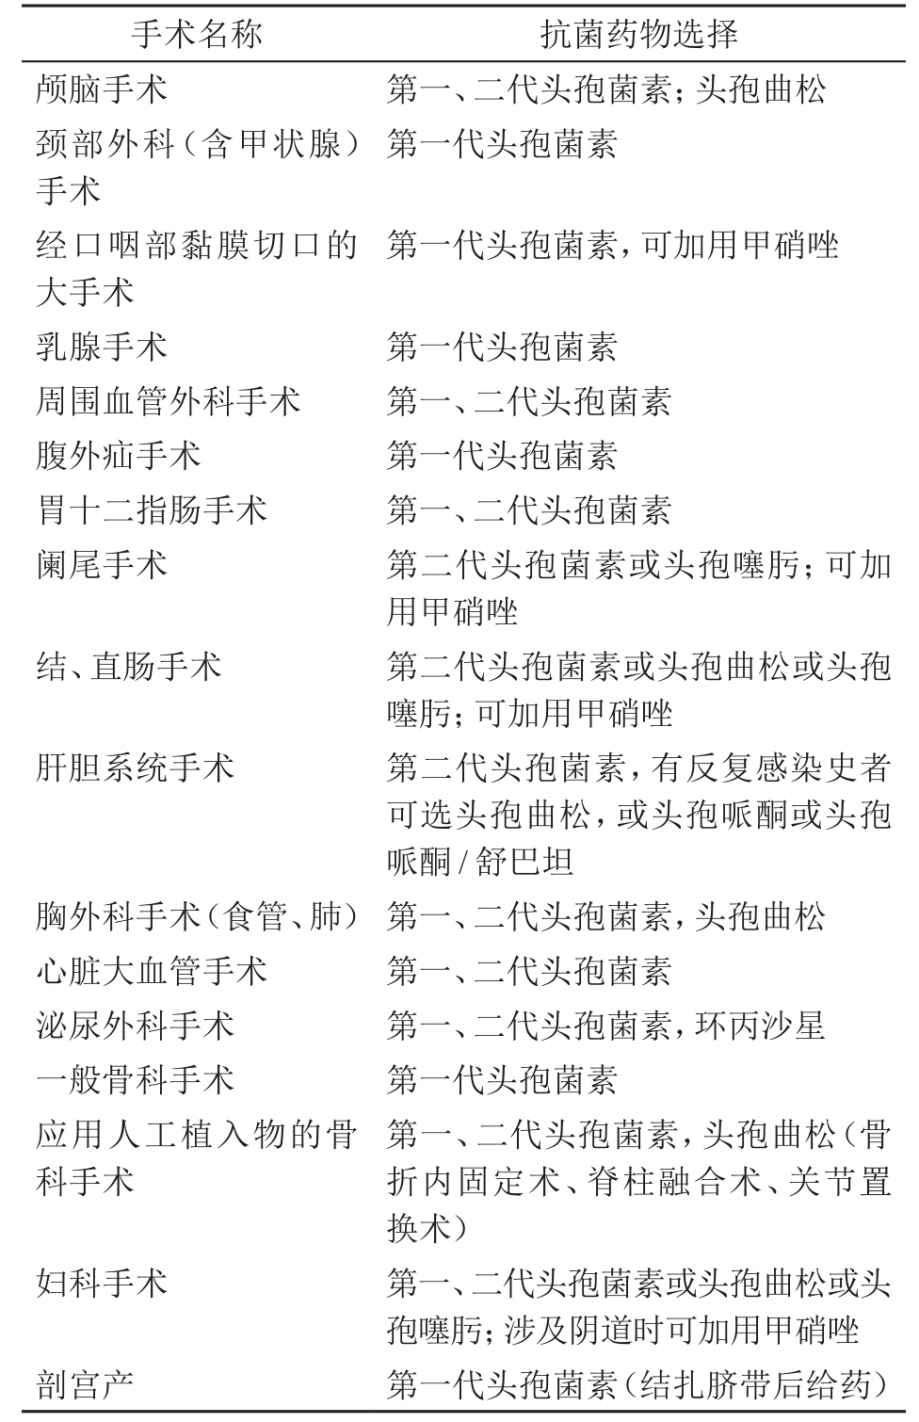
\includegraphics[width=3.23958in,height=5.02083in]{./images/Image00587.jpg}
\end{table}



\protect\hypertarget{text00432.html}{}{}

\section{抗菌药物的联合应用}

\subsubsection{抗菌药物联合应用的结果}

抗菌药物联合在体外或动物实验中可以获得“无关”、“累加”、“协同”、“拮抗”四种作用,在人体内除非有严格对照的临床试验,这些作用不易判断或鉴别。无关作用指总的作用不超过联合中作用较强者,也即两药联合后未取得结果,这在体外试验中比较常见;两种抗菌药物联合的结果相当于两者作用相加的总和时称为累加作用或相加作用;这也是一种较常见的现象;若两药合用时所得的效果比两药作用相加时为好,则称为协同作用,少见;拮抗作用最少见,乃指两药合用时其结果仅较联合中作用较强者独用时为差,即作用互有抵消。

随着抗菌药物作用机制研究的进展,目前可将抗菌药物分为四大类:第一类为繁殖期杀菌剂如青霉素类、头孢菌素类、万古霉素等;第二类为静止期杀菌剂如氨基糖苷类、多黏菌素类(对繁殖期和静止期细菌均具杀灭作用)等;第三类为快效抑菌剂如四环素类、氯霉素类、大环内酯类等;第四类为慢效抑菌剂如磺胺药、TMP、环丝氨酸等。第一类与第二类合用常可获得协同作用,乃由于细菌细胞壁的完整性被破坏后,第二类药物易于进入细胞内作用于靶位所致。第三类药物可迅速阻断细菌的蛋白质合成,以致细菌处于静止状态,因此与第一类药物合用时有导致其抗菌活性减弱的可能。第三类与第二类合用常可获得累加或协同作用。第三类与第四类合用常可获得累加作用。第四类药物对第一类无重要影响,合用后能产生累加或无关作用。

\subsubsection{抗菌药物联合应用的适应证}

对多数单一细菌感染时,应尽量选用一种针对性的药物,单一药物的药敏结果与临床疗效的符合率约80\%左右,两者的关系也较为肯定。临床上多数感染用一种抗菌药物即可获得控制,联合应用抗菌药物仅适用于少数情况(表\ref{tab154-2})。滥用抗菌药物联合可引起耐药菌株增加、不良反应增多、易于发生二重感染等不良后果。因此,必须严格掌握联合用药的适应证。

\paragraph{病因未明的严重感染}

尤其发生在慢性病患者、免疫缺陷者、白细胞低下粒细胞缺乏者、病情危重不宜等待时,可在采取有关标本进行细菌培养后即予抗菌药物联合应用,选用药物的抗菌谱宜广。病因未明的化脓性脑膜炎可用大剂量青霉素与氯霉素的联合,其他严重感染可用哌拉西林或头孢菌素与氨基糖苷类的联合,以后可根据细菌培养及药敏结果进行调整。

\paragraph{单一抗菌药物不能控制的严重感染或混合感染}

感染性心内膜炎
、化脓性脑膜炎及发生于免疫缺陷者或粒细胞减少者的各种严重感染如败血症、肺炎等(病原菌已明确),单一抗菌药物常不能有效地控制感染,此时宜联合应用杀菌剂。肠球菌心内膜炎联合应用氨苄西林或青霉素和庆大霉素有明确指征;草绿色链球菌心内膜炎也有联用青霉素和链霉素或庆大霉素的指征。铜绿假单胞菌败血症多发生于严重烧伤后或白血病化疗过程中,致病菌常比较耐药,哌拉西林加氨基糖苷类如庆大霉素、妥布霉素等可发生协同作用,也可考虑联用头孢他啶或头孢哌酮和氨基糖苷类。严重混合细菌感染常见于肠穿孔所致的腹膜炎及胸、腹严重创伤后。肠穿孔后腹膜炎的致病菌常有多种,包括需氧菌或兼性菌如大肠杆菌、产气杆菌、变形杆菌属、铜绿假单胞菌、肠球菌属等,和厌氧菌如脆弱类杆菌、消化球菌、消化链球菌等,因此有联用哌拉西林、第二、三代头孢菌素、氨基糖苷类、甲硝唑、克林霉素、氯霉素等的指征。

\paragraph{长期用药有产生耐药可能者}

主要见于两种或三种药治疗结核病;利福平合用其他抗生素治疗金葡菌或表葡菌感染时;可使细菌对抗结核药或利福平不致产生耐药性或延缓产生耐药性。

\paragraph{联合用药使毒性较大药物的剂量得以减少}

两性霉素B与氟胞嘧啶、利福平等合用以治疗深部真菌病时,可将毒性较大的两性霉素B剂量减少,从而减轻毒性反应和有利于疗程的顺利完成。

\begin{table}[htbp]
\centering
\caption{可能有效的抗菌药物联合应用}
\label{tab154-2}
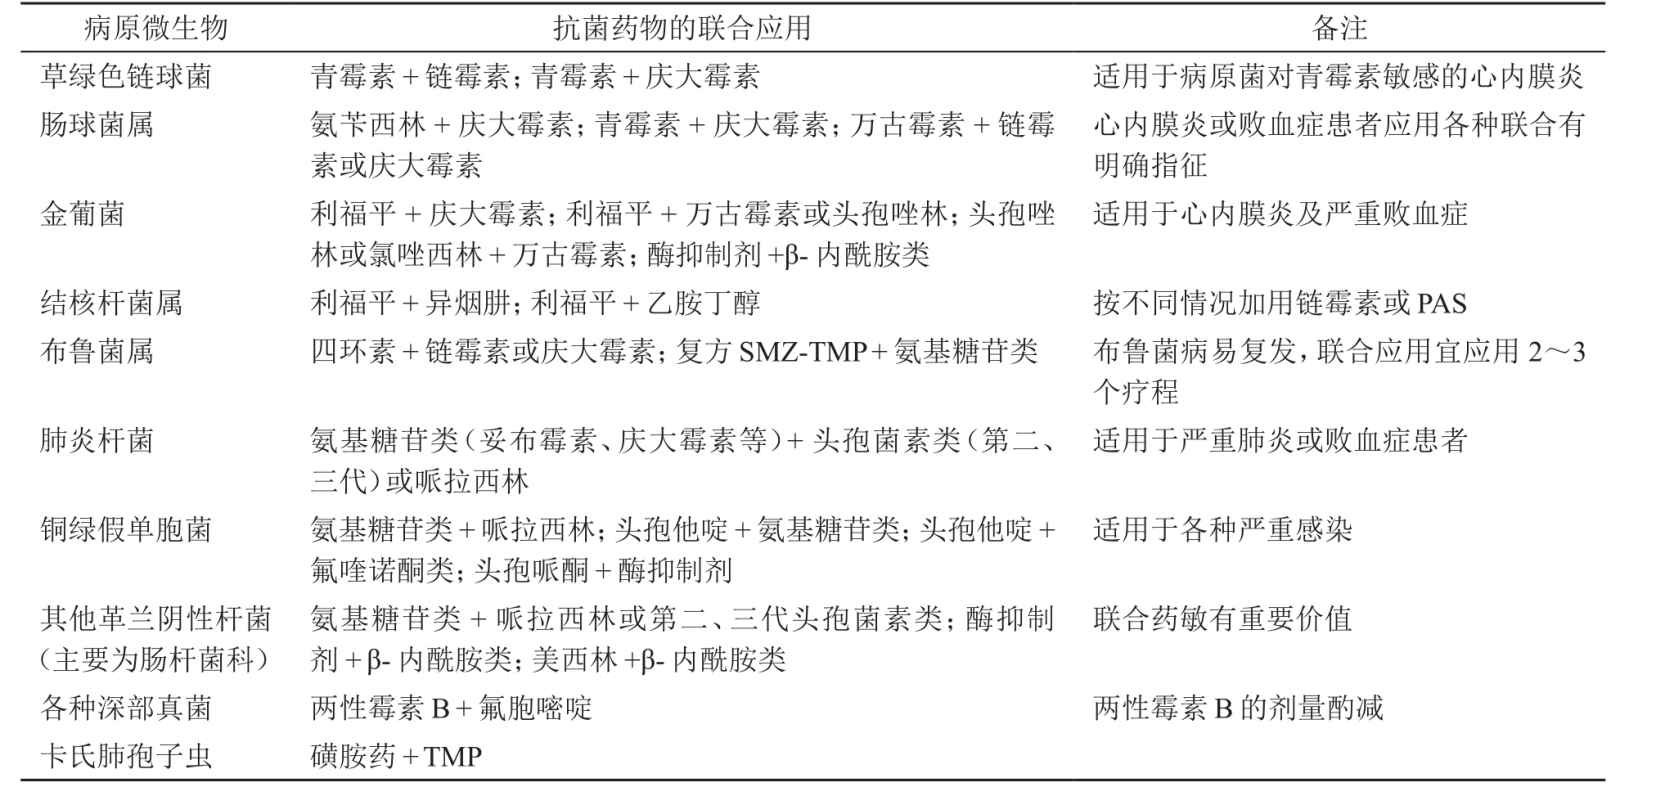
\includegraphics[width=6.8125in,height=3.27083in]{./images/Image00588.jpg}
\end{table}

\paragraph{其他}

加用易于渗入某些组织如中枢神经系统、骨组织等的抗菌药物,能更好地控制感染。治疗细菌性脑膜炎时,除用较大量氨苄西林、青霉素等外,尚可加用磺胺药、氯霉素等易于渗入脑脊液中的药物。治疗金葡菌慢性骨髓炎,除应用青霉素类和头孢菌素类外,尚可加用克林霉素、夫西地酸(褐霉素)、磷霉素、氟喹诺酮类等容易进入骨组织的药物。

\protect\hypertarget{text00433.html}{}{}

\section{抗菌药物的治疗性应用}

抗菌药物的治疗性应用必须有明确的适应证,也即需有较肯定的临床诊断,最好能有病原微生物的证实。在有条件的医院中,对严重而危及生命的一些感染如败血症、感染性心内膜炎、脑膜炎等,应尽一切努力找到病原微生物,并在抗菌药物应用前多次送血作培养(危重病例可每隔1小时采血1次),取脑脊液作涂片和培养,然后按经验治疗给药。分离出病原微生物后迅速检测其药敏和作血清杀菌效价测定,再根据结果调整用药。若无实验室设备,或病情危急必须立即处理时,可推测最可能的病原而进行经验治疗。

抗菌药物依据其体外抗菌活性、药动学参数、不良反应发生率、临床应用效果、细菌耐药性以及药物供应、价格等方面,而被评定为不同病原微生物感染和感染性疾病的首选药物和可选药物,此即所谓“经验治疗”。常见病原微生物感染选择抗菌药物的适应证见表\ref{tab154-3}。

\begin{longtable}{c}
 \caption{抗菌药物的适应证}
 \label{tab154-3}
 \endfirsthead
 \caption[]{抗菌药物的适应证}
 \endhead
 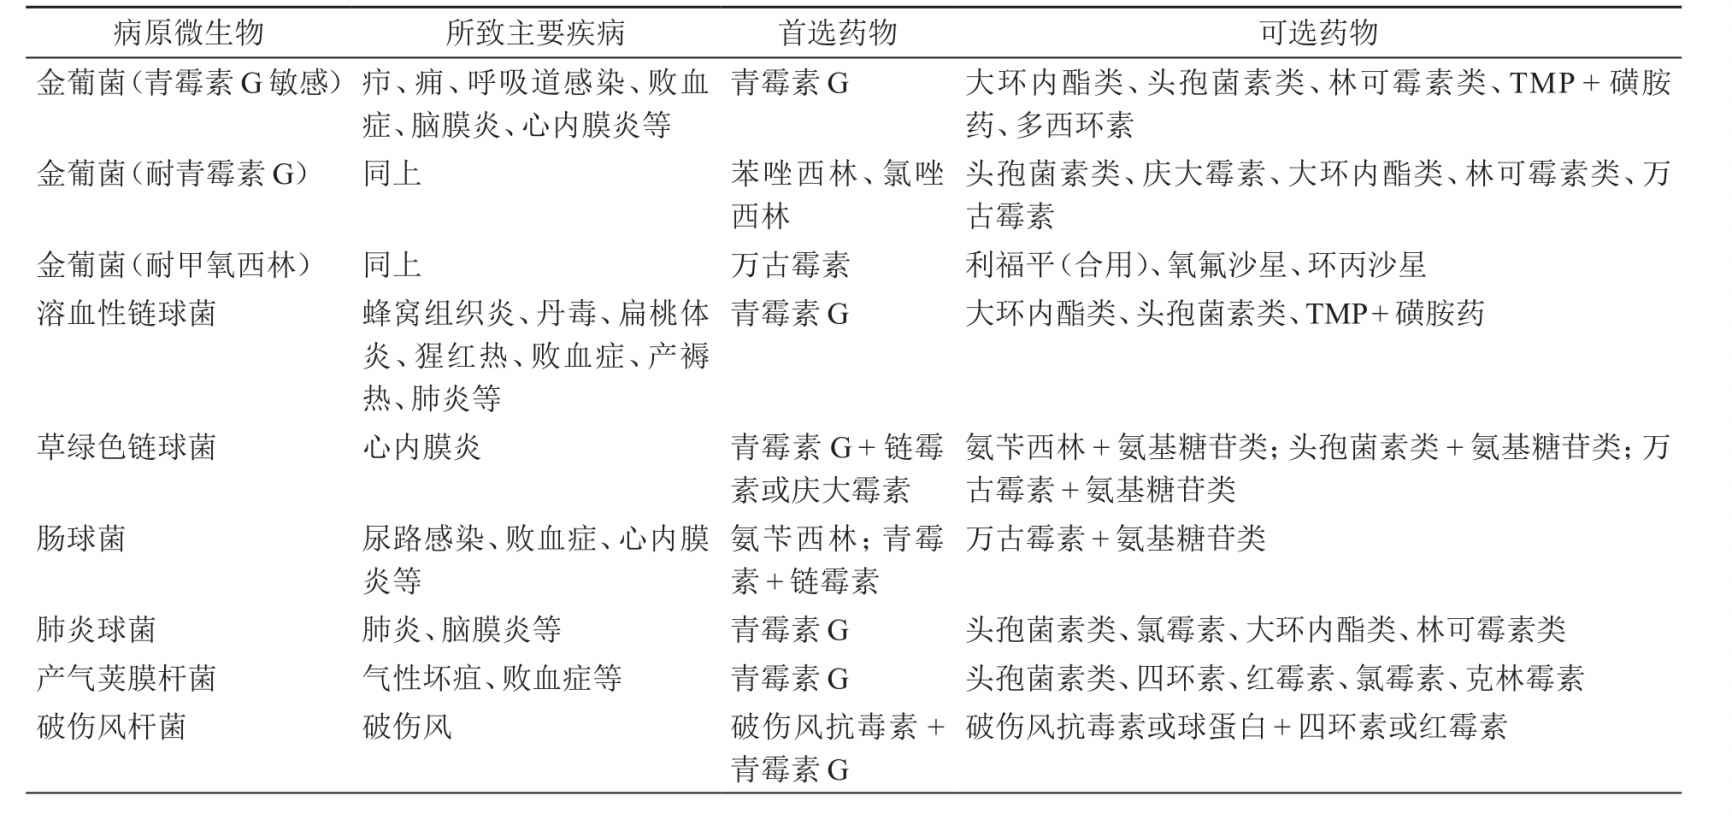
\includegraphics[width=\textwidth,height=\textheight,keepaspectratio]{./images/Image00589.jpg}\\
 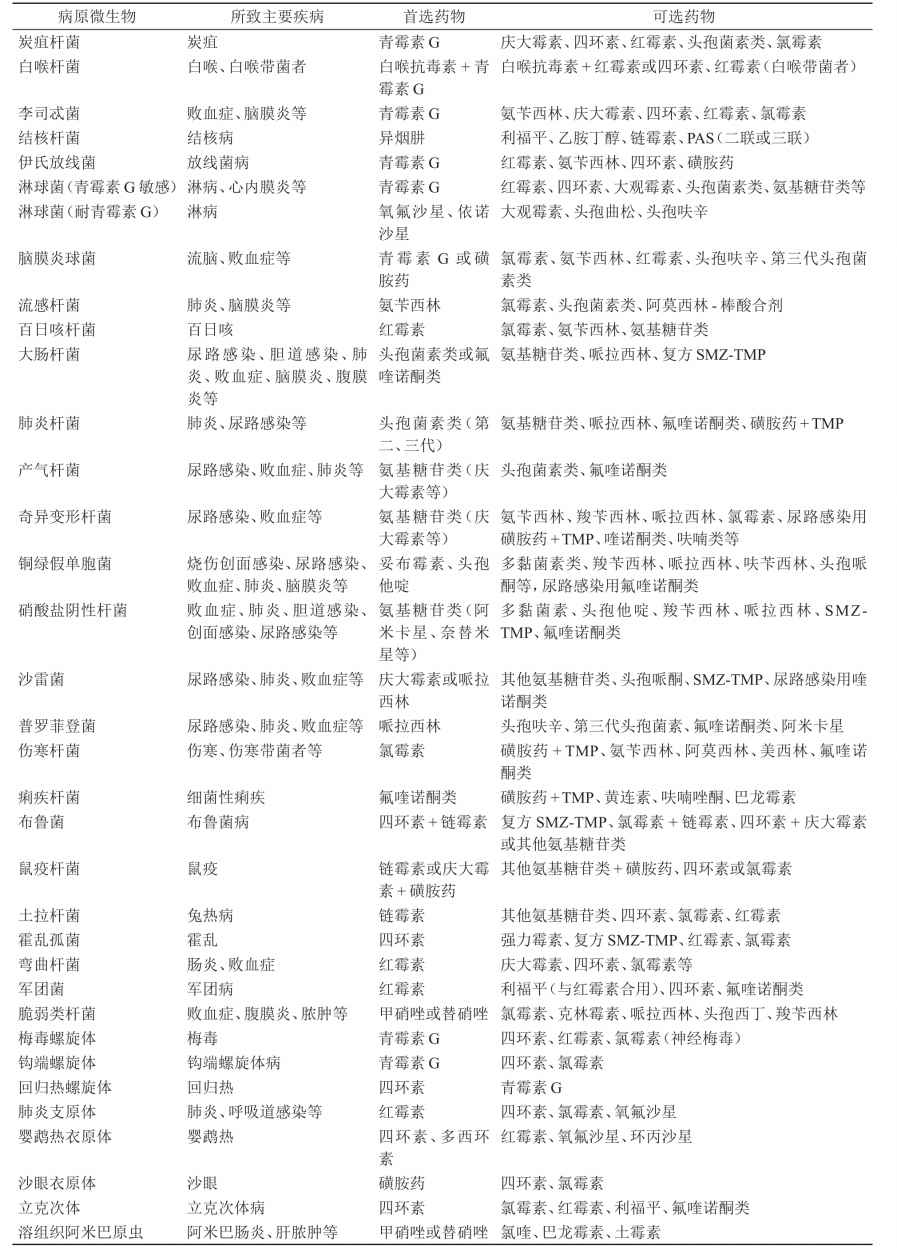
\includegraphics[width=\textwidth,height=\textheight,keepaspectratio]{./images/Image00590.jpg}
 \end{longtable}

\protect\hypertarget{text00434.html}{}{}

\section{抗菌药物在特殊情况下的应用}

\subsubsection{肝功能减退时抗菌药物的应用}

肝病时抗菌药物的选用及其给药方案的制订可参考:①肝功能减退对该类药物的药动学影响;②肝病时该类药物发生毒性反应的可能性。基于此,可将肝病时抗菌药物的应用分为以下几种情况:

1.药物主要由肝脏清除
,肝功能减退时清除明显减少,但并无明显毒性反应发生,故肝病患者仍可应用,但需谨慎,必要时减量给药。属此类情况者有红霉素(不包括红霉素酯化物)、林可霉素、克林霉素等。

2.主要经肝或有相当量药物经肝清除,肝功能减退时药物清除或代谢物形成减少,导致毒性反应发生,此类药物在肝病时宜避免应用。属此类者有氯霉素、利福平、红霉素酯化物、氨苄西林酯化物、异烟肼、两性霉素B、四环素类、磺胺药、酮康唑、咪康唑等。

3.药物经肝
、肾两途径清除,肝功能减退时血药浓度升高,如同时有肾功能损害时则血药浓度更高,严重肝病时需减量应用。属此类者有脲基青霉素类中的美洛西林、阿洛西林和哌拉西林。此外,头孢哌酮、头孢曲松、头孢噻肟、头孢噻吩等亦为经肝、肾排泄的药物,尤以前二者自肝胆系统排出为多,可排出给药量的40\%以上,在严重肝病时,尤其肝肾功能均减退时需减量应用。

4.药物主要由肾排泄,肝功能减退时不需调整剂量氨基糖苷类、青霉素、头孢唑林、头孢他啶、万古霉素、多黏菌素类、氟喹诺酮类(氧氟沙星、环丙沙星、诺氟沙星等)等均属此类情况。可按原治疗量应用。

肝功能减退时抗菌药物的应用详见表\ref{tab154-4}。\footnote{*:活动性肝病时避免应用}

\subsubsection{肾功能减退时抗菌药物的应用}

抗菌药物应用于肾功能减退患者时,其剂量的调整需根据以下因素:①肾功能损害程度;②抗菌药物对肾毒性的大小;③药物的体内过程,即药动学特点;④抗菌药物经血液透析或腹膜透析后可清除的程度。根据抗菌药物体内代谢过程和排泄途径,以及其对肾脏和其他重要脏器毒性的大小,在肾功能减退时药物的选用有以下几种情况。

\paragraph{抗菌药物维持原量或剂量略减}

属此类者主要包括由肝脏代谢或主要自肝胆系统排泄的大环内酯类、利福平、多西环素等;青霉素类和头孢菌素类的部分品种肾肝均为重要清除途径者亦属此类药物。肾功能轻度损害时某些青霉素类如氨苄西林、哌拉西林、苯唑西林和大部分或部分由肝胆系统排泄的头孢哌酮、头孢曲松,以及在体内代谢的头孢噻肟等均可按原治疗量应用,但在肾功能中度以上损害时则需减量使用。氯霉素和两性霉素B虽在肾功能减退时血半减期仅轻度延长,但由于该两药物具有明显的血液系统毒性或肾毒性,因此宜根据病情权衡利弊后再予以减量应用。

\paragraph{剂量需适当调整者}

此类药物无明显肾毒性或仅有轻度肾毒性,但由于排泄途径主要为肾脏,肾功能减退时药物可在体内明显积聚,血半减期显著延长,因此在肾功能轻、中和重度减退时均需根据肾功能减退情况适当调整药物剂量。青霉素类和头孢菌素类的大多品种,如羧苄西林、青霉素、头孢他啶、头孢唑肟、头孢唑林、头孢孟多等均属此种情况;氧氟沙星亦属此类。

\paragraph{剂量必须减少者}

此类药物均有明显肾毒性,且主要经肾排泄。氨基糖苷类、万古霉素、多黏菌素类等均属此类。

\paragraph{肾功能损害时不宜应用者}

包括四环素类(多西环素除外)、呋喃类、萘啶酸等。四环素、土霉素的应用可加重氮质血症;呋喃类和萘啶酸可在体内明显积聚,产生对神经系统的毒性反应。

肾功能减退时抗菌药物的选择应用及其剂量调整分别参见表\ref{tab154-5}\footnote{*:需进行血药浓度监测,或按内生肌酐清除率(或自血肌酐值计算获得)调整给药剂量或给药间期}和表\ref{tab154-6}。

\subsubsection{抗菌药物在老年人中的应用}

随着年龄的增长,机体组织器官的功能也发生改变,抗菌药物的体内过程包括吸收、分布、代谢和排泄等均可在老年期发生某些变化。在多数情况下,老年患者应用抗菌药物后,药物自体内清除减少,血药浓度增高;加上老年患者心血管、呼吸、中枢神经和泌尿生殖系统等原发疾病的增多,使抗菌药物疗程中易发生不良反应。因此在老年人中应用抗菌药物时应注意以下几点:

\paragraph{尽量避免使用毒性大的抗菌药物}

如确有指征应用该类药物时需调整给药方案。此类药物一般治疗浓度范围狭窄,即治疗药物浓度与中毒浓度相差小,且个体差异亦大。氨基糖苷类和万古霉素属此类药物。此时应进行血药浓度监测,据此调整剂量,使给药方案个体化,以达到用药安全、有效的目的。

\paragraph{老年患者可减量应用毒性低的 β-内酰胺类抗生素}

青霉素类、头孢菌素类、氨曲南等虽毒性低微,但大多主要自肾排泄,老年患者的药物清除明显减少,血半减期延长。因此,须减量应用。应按轻度肾功能减退情况减量给药,可用正常治疗量的2/3~1/2。

\begin{table}[htbp]
\centering
\caption{肝功能减退感染患者抗菌药物的应用}
\label{tab154-4}
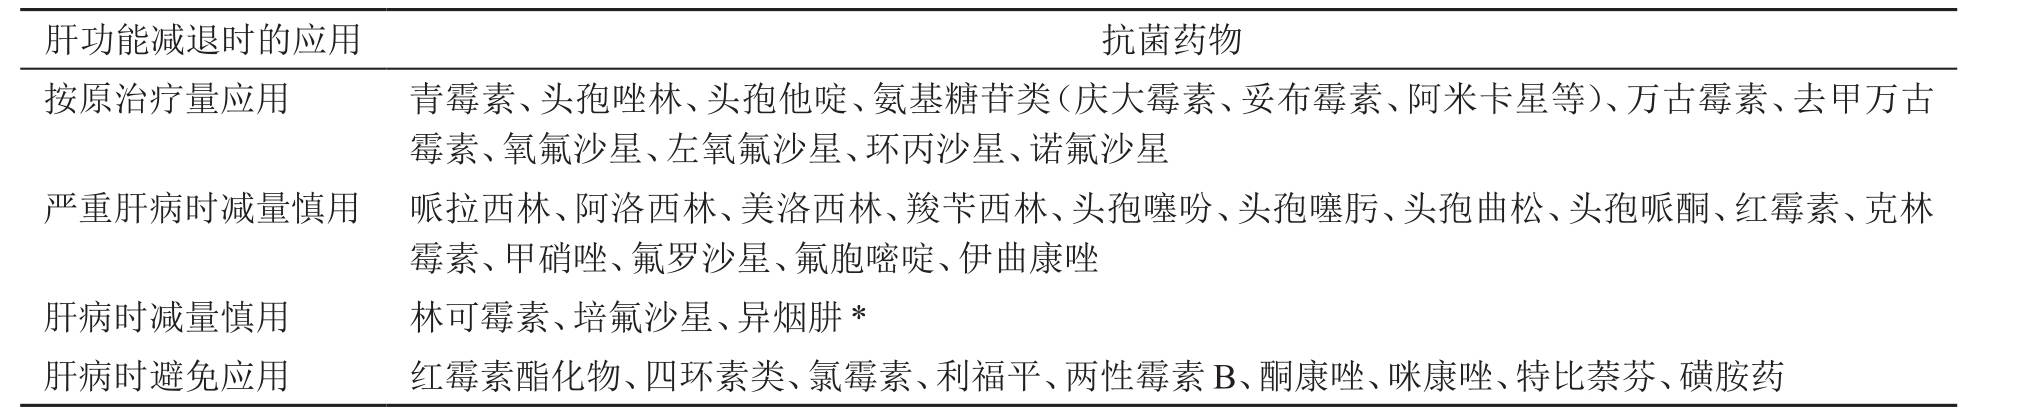
\includegraphics[width=6.71875in,height=1.375in]{./images/Image00591.jpg}
\end{table}

\begin{table}[htbp]
\centering
\caption{肾功能减退感染患者抗菌药物的应用}
\label{tab154-5}
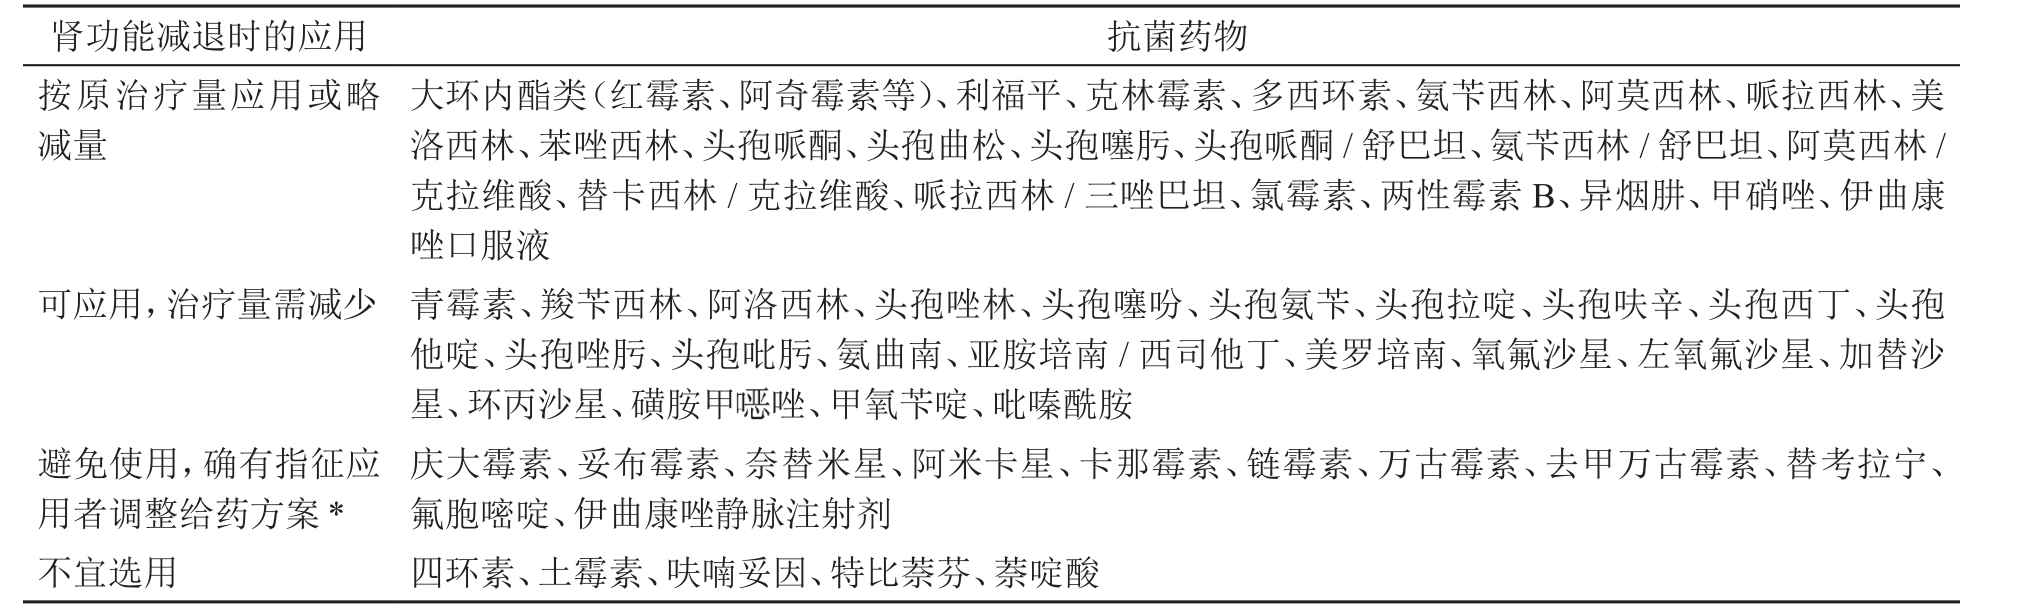
\includegraphics[width=6.73958in,height=2.04167in]{./images/Image00592.jpg}
\end{table}

\begin{longtable}{c}
 \caption{肾功能衰竭时抗菌药物的剂量调整\textsuperscript{(1)}}
 \label{tab154-6}
 \endfirsthead
 \caption[]{肾功能衰竭时抗菌药物的剂量调整\textsuperscript{(1)}}
 \endhead
 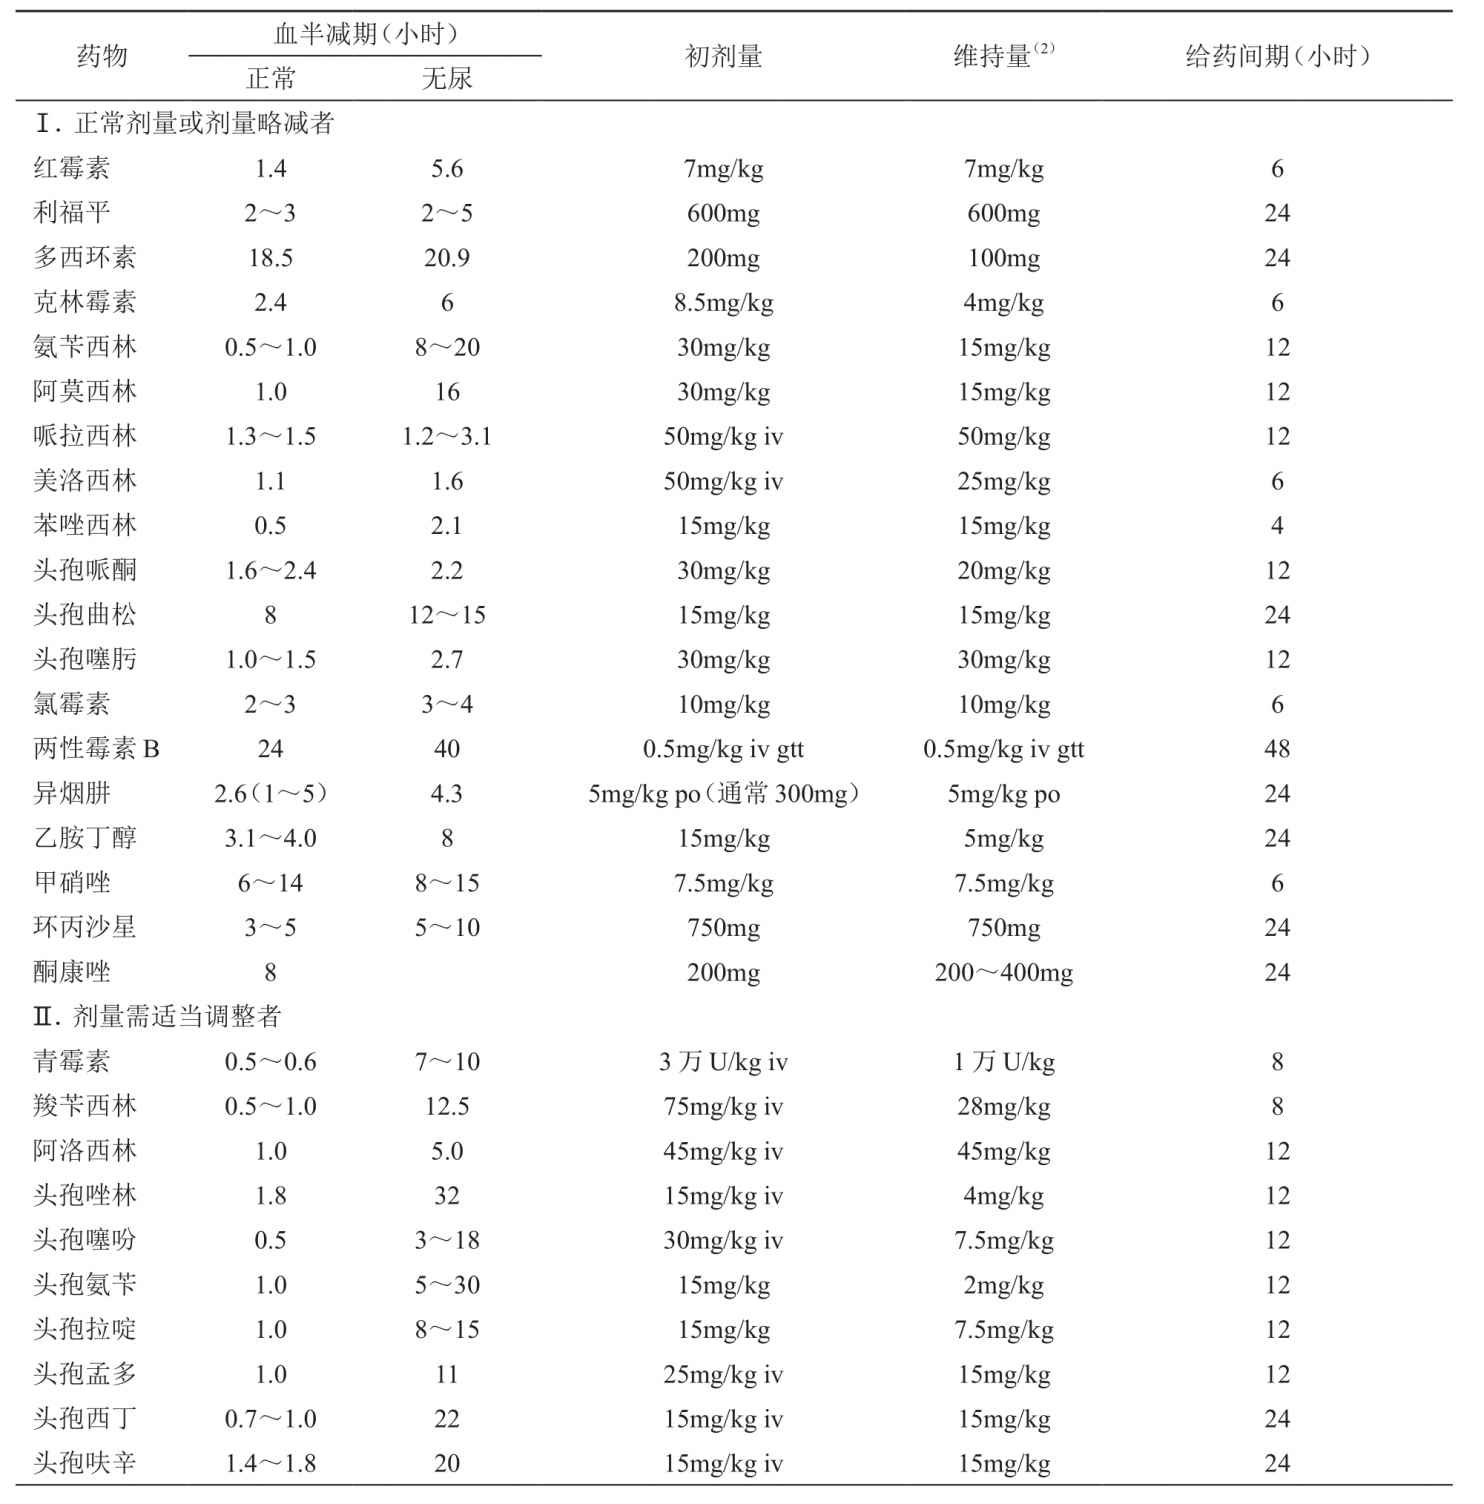
\includegraphics[width=\textwidth,height=\textheight,keepaspectratio]{./images/Image00593.jpg}\\
 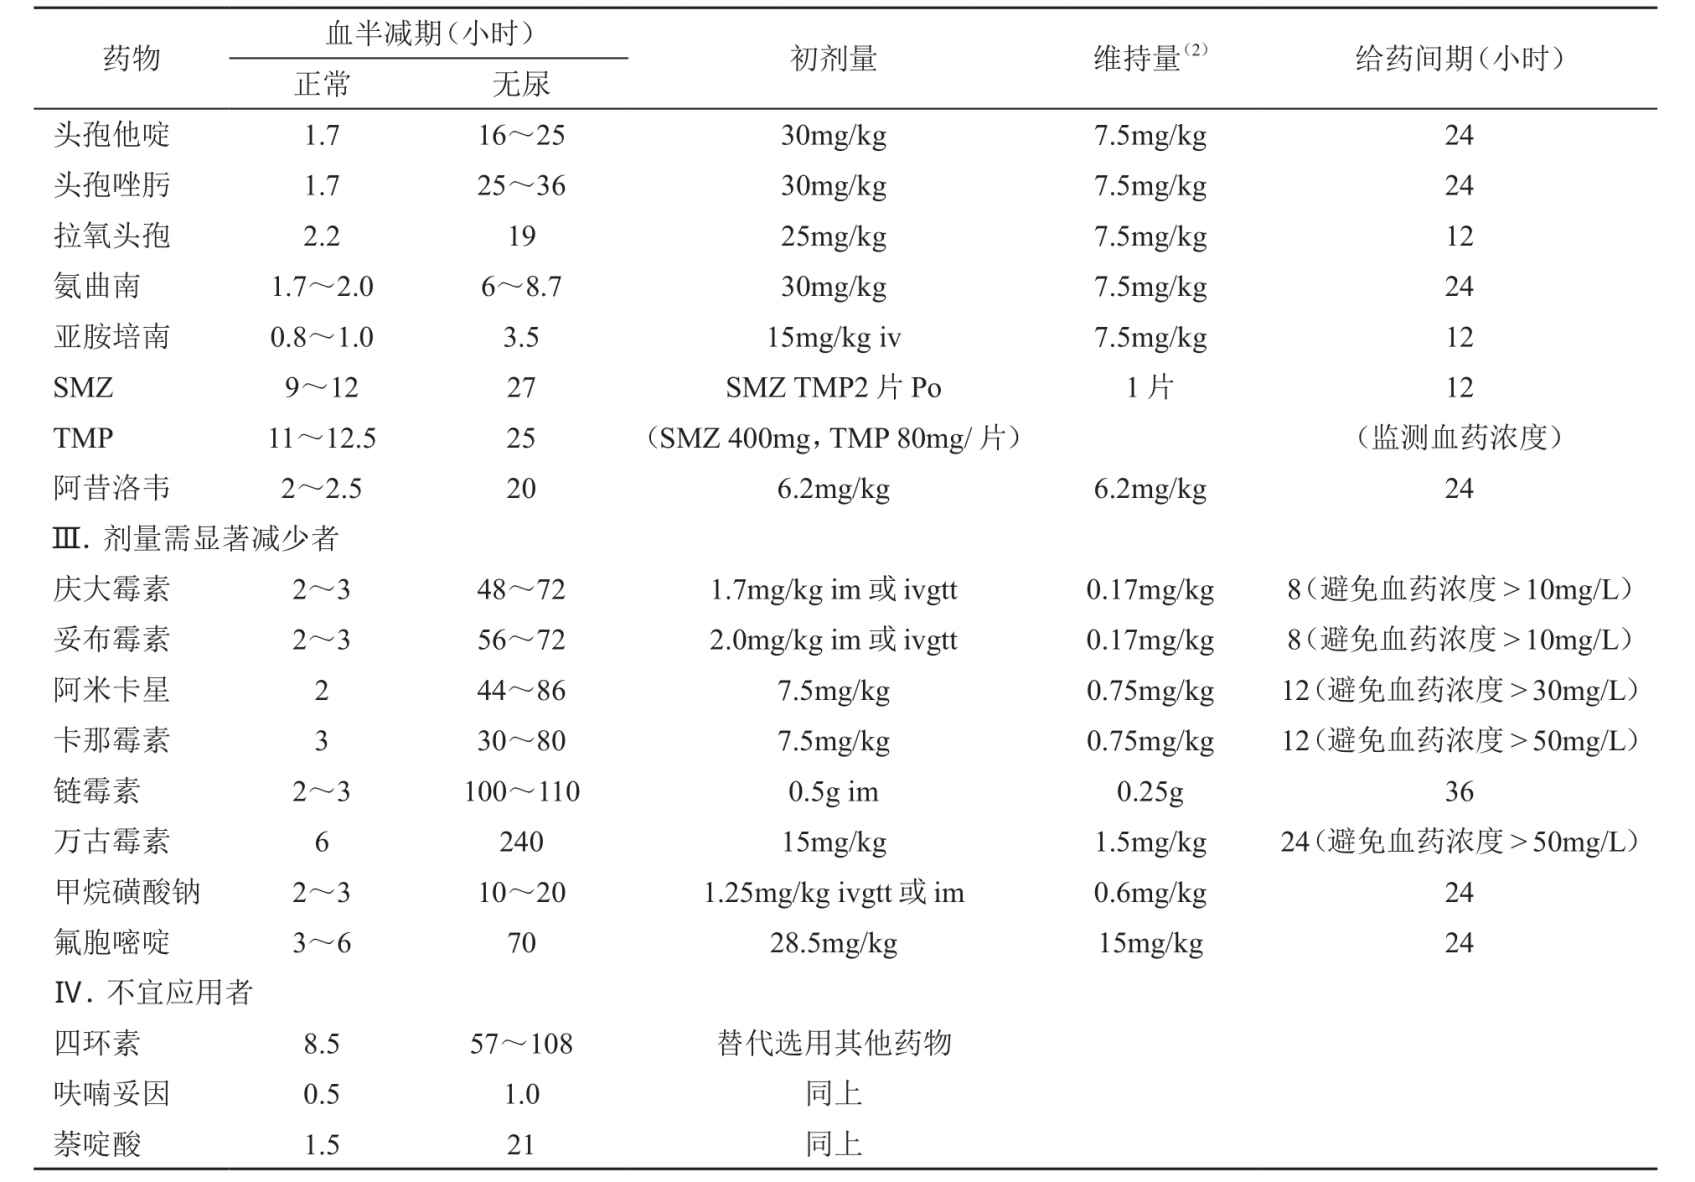
\includegraphics[width=\textwidth,height=\textheight,keepaspectratio]{./images/Image00594.jpg}
\end{longtable}

注:(1) 此维持量为内生肌酐廓清率<
5ml/min时的每次用量,如肾功能损害较此为轻时,剂量可酌情增大。

(2) 当血肌酐值> 12mg/kg时,慢乙酰化者剂量需减少为每日200mg

\paragraph{老年人感染宜用杀菌剂}

由于免疫功能降低和组织器官功能退化,病灶内细菌的清除更有赖于抗菌药物的杀菌作用,氨基糖苷类、青霉素类和头孢菌素类均为可选药物,但仍应按患者肾功能情况调整给药剂量和间期。

\subsubsection{抗菌药物在新生儿中的应用}

新生儿体内酶系发育不完全,血浆蛋白结合药物的能力较弱,GFR较低(尤以β-内酰胺类和氨基糖苷类的排泄较慢),故按体重计算抗菌药物用量后,其血药(尤其是游离部分)浓度比年长儿和成人为高,血药半减期也见延长,因此给药间期一般比成人或年长儿为长。上述情况主要适用于毒性低、主要由肾排泄的β-内酰胺类抗生素。出生30天期间,新生儿的酶系、肝、肾功能不断发育而臻完善,因此宜按日龄而调整剂量或给药间期(表\ref{tab154-7})。此外,尚须注意以下几点:

1.新生儿期由于肝酶系统的不足
,肾排泄能力的不完备,一些毒性大的抗菌药物,如主要经肝代谢的氯霉素、磺胺药,主要自肾排泄的氨基糖苷类、万古霉素、多黏菌素类、四环素类等均应尽量避免应用。如确有指征应用氨基糖苷类、氯霉素等时,必须有血药浓度监测,并个体化给药,以保证治疗安全有效。万古霉素、多黏菌素类、四环素类、磺胺药、呋喃类均不宜选用(表\ref{tab154-8})。

2.氟喹诺酮类药物在新生儿中禁用。

3.新生儿应用抗菌药物时不宜肌注给药。

\subsubsection{抗菌药物在小儿患者中的应用}

小儿患者在应用抗菌药物时应注意以下几点:①氨基糖苷类抗生素:该类药物有明显耳、肾毒性,小儿患者应尽量避免应用。临床有明确应用指征且又无其他毒性低的抗菌药物可供选用时,方可选用该类药物,并在治疗过程中严密观察不良反应。有条件者应进行血药浓度监测,个体化用药。②万古霉素和去甲万古霉素:该类药也有一定肾、耳毒性,小儿患者仅在有明显指征时方可选用,并应进行血药浓度监测,个体化给药。③四环素类抗生素:不可用于8岁以下小儿。④氟喹诺酮类抗菌药:该类药物避免用于18岁以下未成年人。

\subsubsection{妊娠期抗菌药物的应用}

孕妇应用抗菌药物时必须考虑到药物对母体和胎儿两方面的影响,尤其是对胎儿的影响。进入胎儿体内的抗菌药物按其对胎儿的影响可分为以下几类:

\paragraph{有致畸或明显毒性的药物妊娠期须禁用}

属此类药物者有:①四环素类;②磺胺药;③TMP和乙胺嘧啶,两药均可抑制叶酸代谢,并有致畸可能,妊娠期不宜应用,妊娠早期列为禁用;④氯霉素;⑤甲硝唑,对动物有致突变作用,妊娠早期禁用;⑥利福平,对小鼠有致畸作用,早期不可应用;⑦金刚烷胺、碘苷、阿糖腺苷,前者有致畸作用,后两者有致突变和致癌作用,不可应用。

\begin{table}[htbp]
{\centering
\caption{新生儿的抗菌药物剂量和用法}
\label{tab154-7}
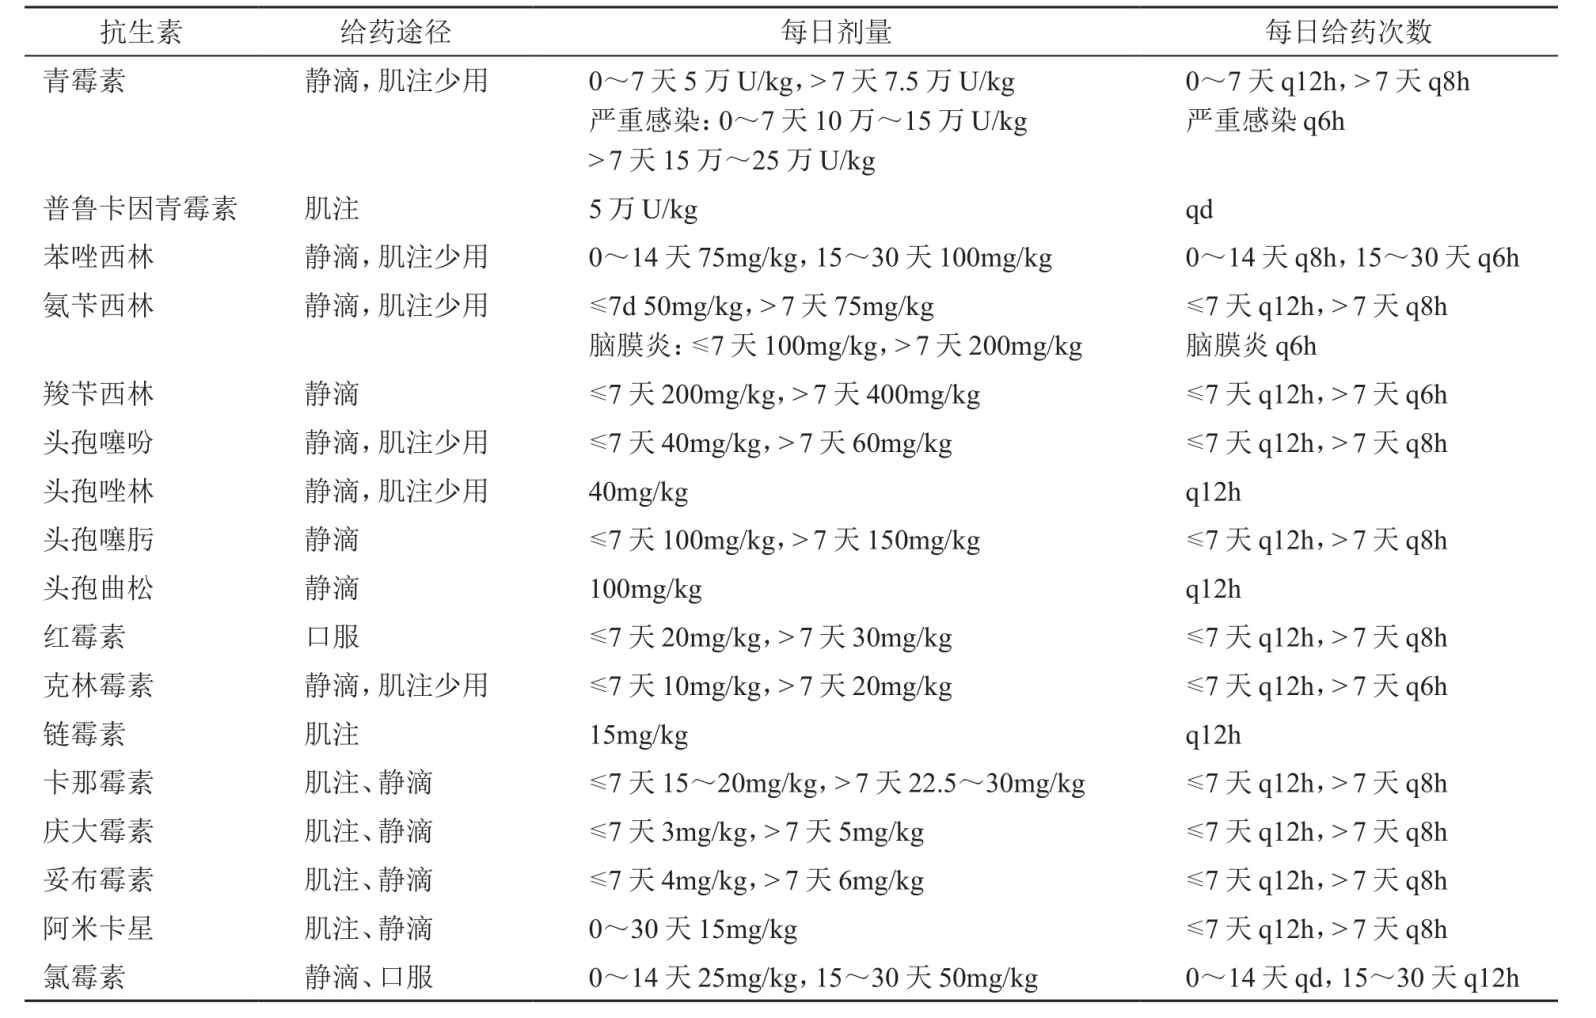
\includegraphics[width=6.70833in,height=4.27083in]{./images/Image00595.jpg}}

{\small 
注:(1) 早产儿或出生体重≤2kg者,每日剂量略减,给药间期需延长。

(2)
氨基糖苷类及氯霉素先参考此表剂量及用法给药,以后需进行血药浓度监测再加以调整,无监测条件者不宜应用
}
\end{table}


\begin{table}[htbp]
\centering
\caption{新生儿应用抗菌药物后可能引起的不良反应}
\label{tab154-8}
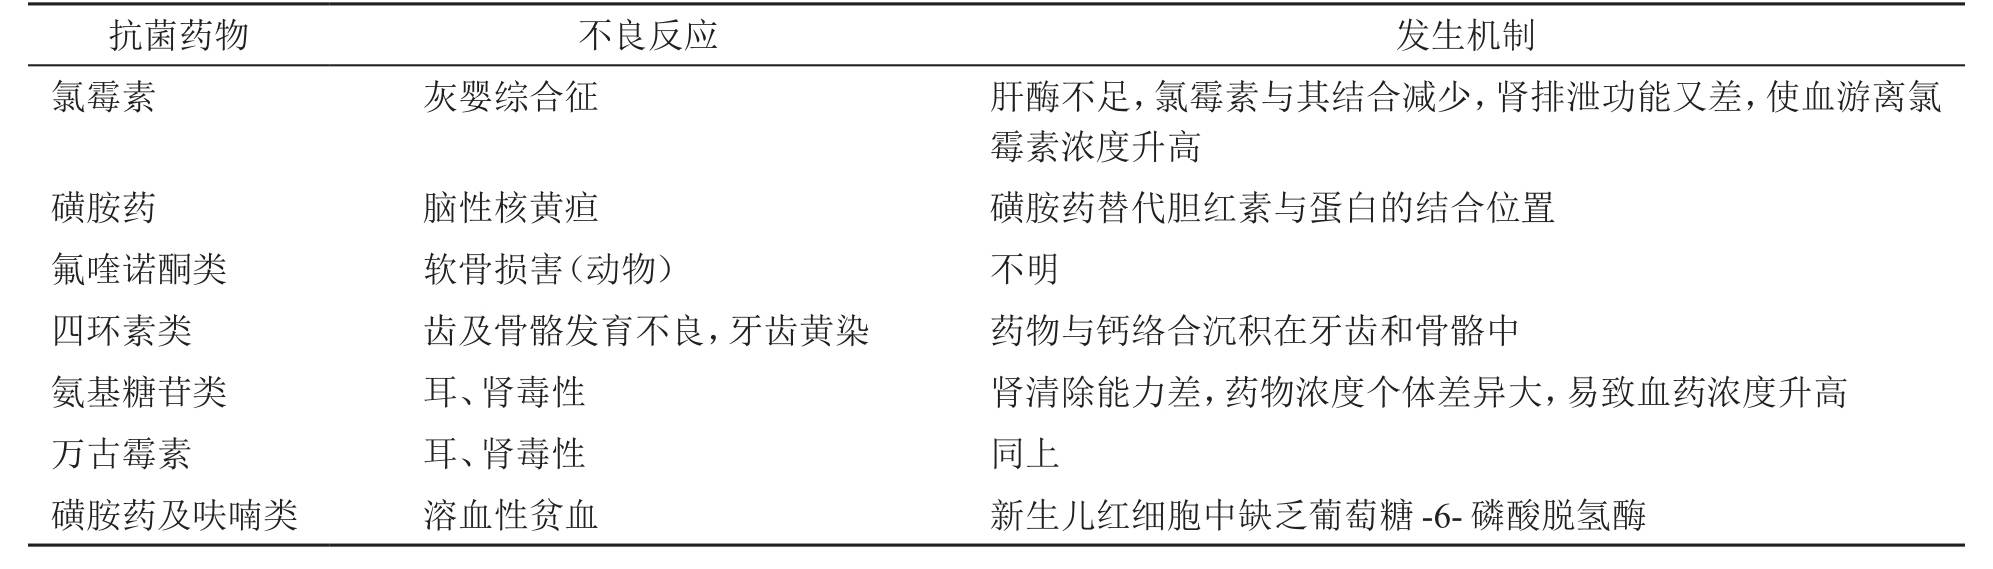
\includegraphics[width=6.63542in,height=1.88542in]{./images/Image00596.jpg}
\end{table}

\paragraph{药物对母体和胎儿有一定毒性或影响者应避免在妊娠全过程中应用}

其中某些抗菌药物如有绝对指征应用时则可充分权衡利弊后再予以采用。属于此类的药物有:①氨基糖苷类;②万古霉素;③喹诺酮类;④异烟肼,易透过血胎盘屏障,干扰维生素B\textsubscript{6}
的代谢,引起中枢神经系统的损害,应避免应用。有指征应用时需加用维生素B\textsubscript{6}
;⑤氟胞嘧啶,对动物有致畸作用,人类中未证实;⑥呋喃妥因,可致溶血反应,避免应用。

\paragraph{妊娠期间可选用的药物}

此类药物毒性低,或对胎儿无明显影响,也无致畸作用。包括:①青霉素类、头孢菌素类、其他β-内酰胺类;②大环内酯类,除红霉素酯化物外,红霉素、麦迪霉素等均无显著毒性,也不易透过血胎盘屏障,故可考虑应用;③林可霉素和克林霉素,未发现对胎儿有明显影响,妊娠期可应用;④磷霉素,毒性低微,可应用。

妊娠各期避免或可选用的抗菌药物见表\ref{tab154-9}。抗菌药物在妊娠期应用时的危险性分类见表\ref{tab154-10}。

\subsubsection{哺乳期时抗菌药物的应用}

乳妇应用抗菌药物时对乳儿的影响与以下两因素有关,即药物分泌至乳汁中的量,以及乳儿可自乳汁中摄入的药量;后一因素取决于药物是否可自胃肠道吸收和吸收量的多少。抗菌药物在乳汁中的浓度见表\ref{tab154-11}。

乳妇患者接受抗菌药物后,药物可自乳汁分泌,通常母乳中药物含量不高,不超过哺乳期患者每日用药量的1\%;然而无论乳汁中药物浓度如何(参见表\ref{tab154-11}),均存在对乳儿潜在的影响,并可能出现不良反应,如氨基糖苷类抗生素可导致乳儿听力减退,氯霉素可致乳儿骨髓抑制,SMZ等可致核黄疸、溶血性贫血,四环素类可致乳齿黄染,青霉素类可致过敏反应等。因此治疗乳妇患者时应避免选用氨基糖苷类、喹诺酮类、四环素类、氯霉素、磺胺药等。哺乳期患者应用任何抗菌药物时,均宜暂停哺乳。

\begin{table}[htbp]
\centering
\caption{妊娠期抗菌药物的选择}
\label{tab154-9}
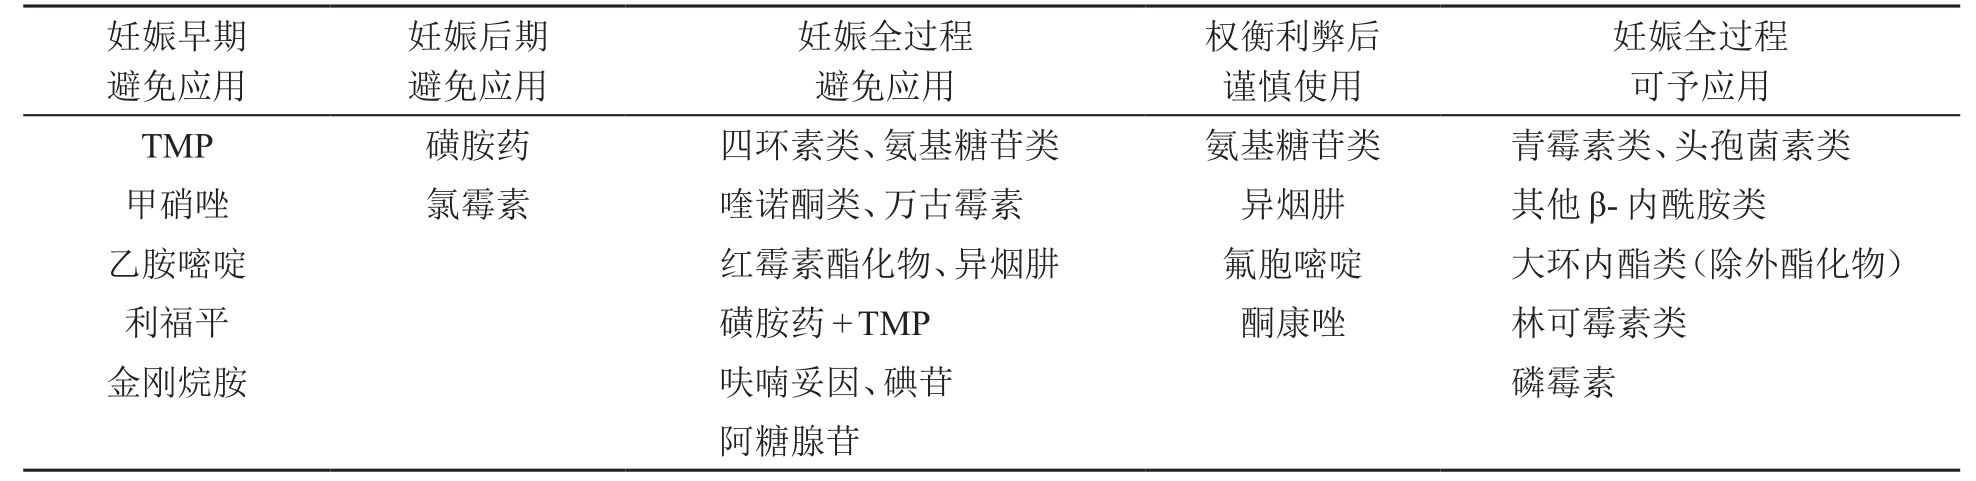
\includegraphics[width=6.58333in,height=1.59375in]{./images/Image00597.jpg}
\end{table}

\begin{table}[htbp]
{\centering
\caption{抗菌药物在妊娠期应用时的危险性分类}
\label{tab154-10}
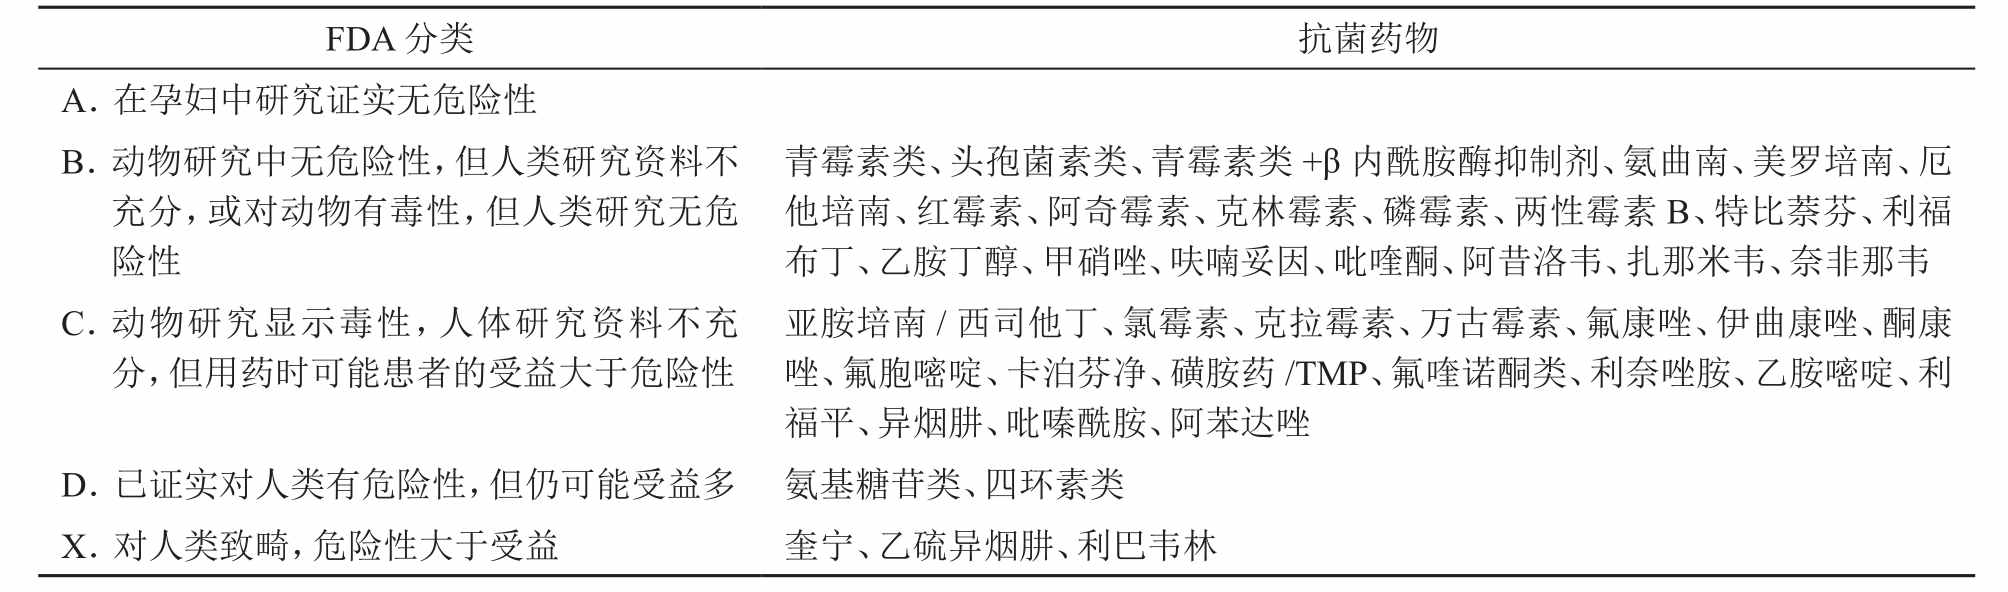
\includegraphics[width=6.6875in,height=1.95833in]{./images/Image00598.jpg}}

{\small 
注:(1)
妊娠期感染时用药可参考表中分类,以及用药后患者的受益程度及可能的风险,充分权衡后决定。A类:妊娠期患者可安全使用;B类:有明确指征时慎用;C类:在确有应用指征时,充分权衡利弊决定是否选用;D类:避免应用,但在确有应用指征、且患者受益大于可能的风险时严密观察下慎用;X类:禁用。

(2)
妊娠期患者接受氨基糖苷类、万古霉素、去甲万古霉素、氯霉素、磺胺药、氟胞嘧啶时必须进行血药浓度监测,据以调整给药方案
}
\end{table}



\begin{table}[htbp]
\centering
\caption{抗菌药物在乳汁中的浓度}
\label{tab154-11}
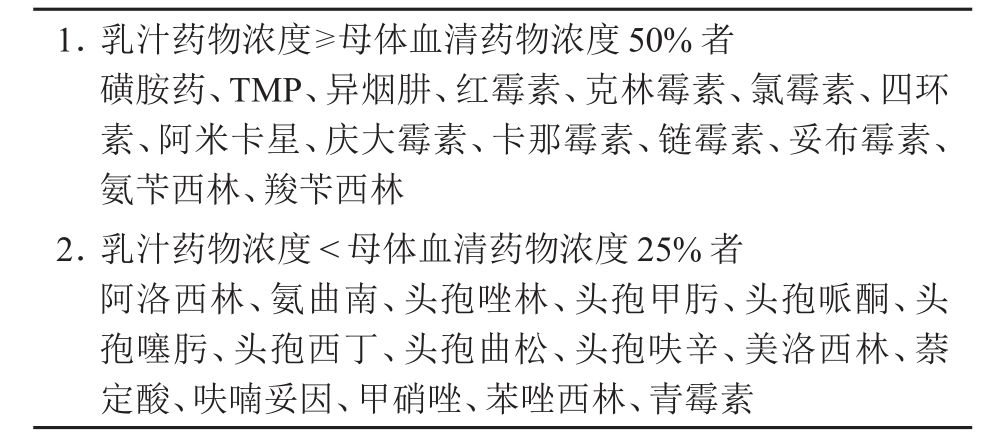
\includegraphics[width=3.26042in,height=1.48958in]{./images/Image00599.jpg}
\end{table}

\subsubsection{抗菌药物在免疫缺陷者感染中的应用}

正常人具有物理的和化学的屏障、非特异性免疫和特异性免疫功能以防御各种病原体的入侵;任何影响和损伤这些免疫功能的因素,皆可使人易于发生感染,称为免疫缺陷者感染。获得性免疫缺陷者感染,即由创伤、异物、营养不良、肿瘤、脾切除、药物和某些病原体等所致免疫缺陷而产生的感染。免疫缺陷者最常见感染部位为口腔、肺、尿道、肛周区和皮肤软组织,大肠杆菌、金葡菌、表皮葡萄球菌、铜绿假单胞菌、肺炎杆菌、肠球菌属、硝酸盐阴性杆菌和阴沟杆菌等为最常见的致病菌。感染部位与致病微生物之间有密切关系:口咽和食管炎主要为白色念珠菌,偶也可由金葡菌引起;肺炎大多由革兰阴性杆菌或者是金葡菌、表皮葡萄球菌和肠球菌属所致,较长期应用广谱抗菌药物者则曲菌属、念珠菌属等感染也有可能;白血病患者肛周感染的致病菌大多为铜绿假单胞菌,而皮肤软组织感染则多由金葡菌或表皮葡萄球菌所致。

免疫缺陷者感染抗菌药物应用的基本原则是:

1.尽早开始经验治疗
应选用广谱、高效、低毒的抗菌药物经验疗法。在应用强有力抗菌药物情况下,患者体温不降或下降后又有上升,应考虑真菌感染,可选用酮康唑、伊曲康唑、氟康唑和氟胞嘧啶,必要时用两性霉素B。

2.根据病原微生物选择抗菌药物
在抗菌药物治疗开始前留取的标本获得阳性结果时,可根据病原菌的药敏选择更合适的药物。

3.选用的抗菌药物应具备下列条件
①为杀菌剂;②对病原体有高度活性;③在感染部位可达到有效治疗浓度;④对细胞内微生物有作用;⑤不易导致耐药菌出现;⑥毒性低;⑦可由需要途径给药。在合理选用抗菌药物基础上,采用两种药物联合治疗,从而起到协同作用。

4.抗菌药物应用宜静脉给药、足量和连续静滴
因为此类患者感染的病原微生物清除完全依靠药物,机体缺乏免疫防御能力,一旦抗菌药物在感染部位消失,细菌可立即繁殖,若能较长时间保持有效血或组织抗菌药物浓度,则有利于杀灭细菌。

5.纠正免疫缺陷。

\protect\hypertarget{text00435.html}{}{}

\section{抗菌药物的相互作用}

药物相互作用系指两种以上药物同用时,其中某一种(或一种以上)药物的作用受到干扰或影响,使该药的疗效发生变化或产生毒性反应。抗菌药物是使用较广泛的一类药物,常与另一种抗菌药物或其他药物合用,因而每有发生相互作用的可能。有作用加强和作用减弱两种结果,临床上作用加强可表现为疗效提高(协同作用等)或毒性加大,作用减弱可表现为疗效降低(拮抗作用等)或毒性减轻。在合用多种药物时应力求避免某药的疗效降低或(和)毒性加大,而力争获得疗效提高或(和)毒性减轻的良好效果。

相互作用的发生机制有:

1.直接理化作用
该作用主要发生在体外,一部分发生在体内,其中尤以口服为多。在输液中,抗菌药物间及与其他药物间常可发生相互作用(通常称为配伍禁忌),其最后结果常使抗菌药物的活性明显减弱,此外尚可出现溶液混浊、变色、沉淀等。常用抗菌药物如青霉素类、四环素类、头孢菌素类、多黏菌素类等,均宜单独静注或静滴。

2.血清蛋白质结合点的竞争与置换
主要见于磺胺药,如磺胺药与口服降糖药和抗凝剂等合用,可因置换作用而导致这些药物的游离部分浓度增高,引起了低血糖和出血。

3.药物代谢酶的诱导(酶促)或抑制(酶抑)。

4.肾小管和胆道分泌的竞争。

5.在组织部位的相互作用。

抗菌药物的相互作用详见表\ref{tab154-12}。

\begin{longtable}{c}
 \caption{抗菌药物的相互作用(包括配伍禁忌)}
 \label{tab154-12}
 \endfirsthead
 \caption[]{抗菌药物的相互作用(包括配伍禁忌)}
 \endhead
 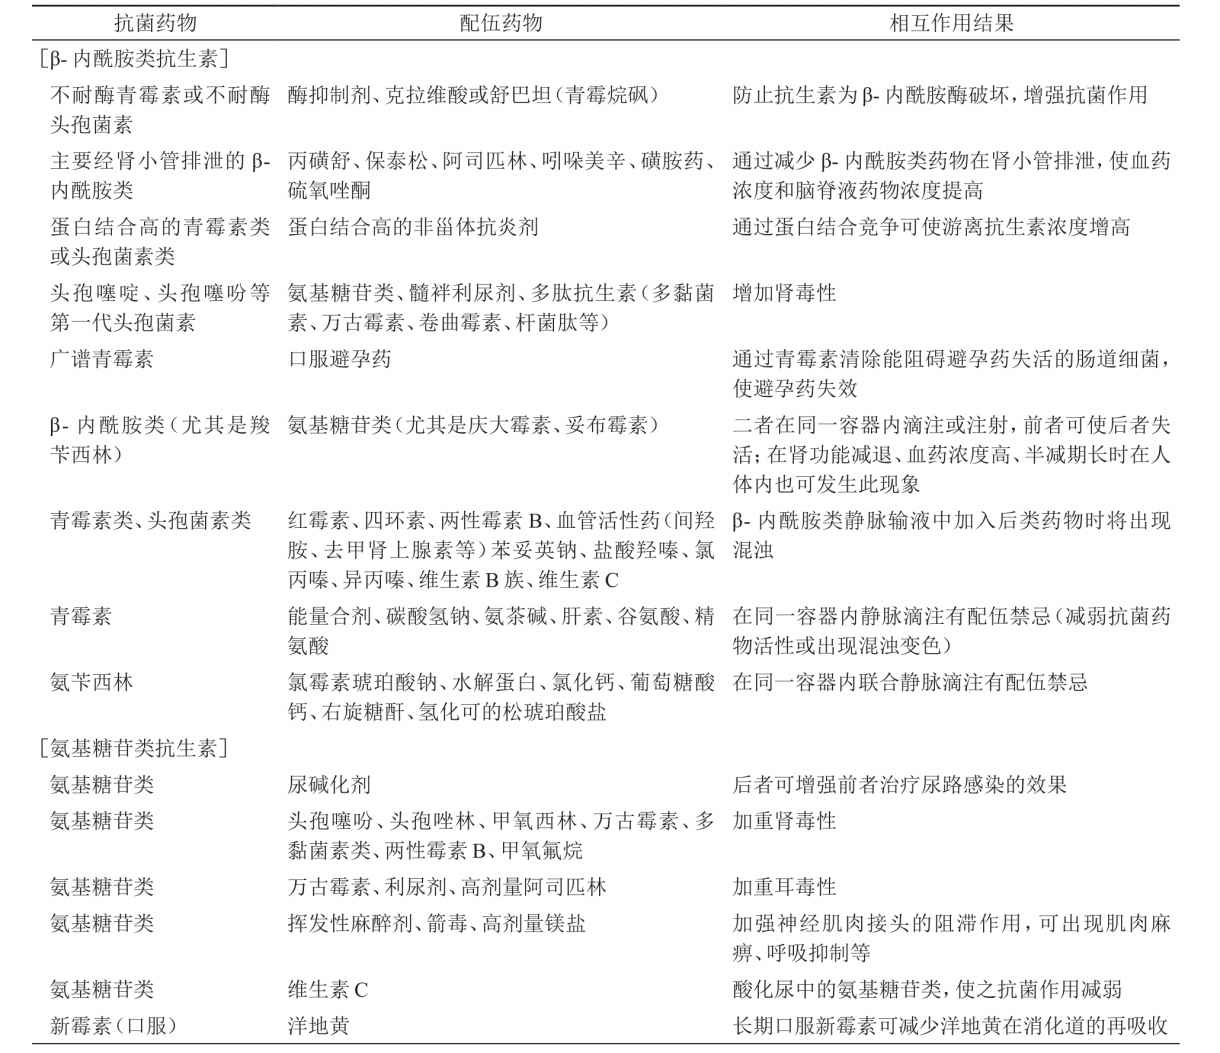
\includegraphics[width=\textwidth,height=\textheight,keepaspectratio]{./images/Image00600.jpg}\\
 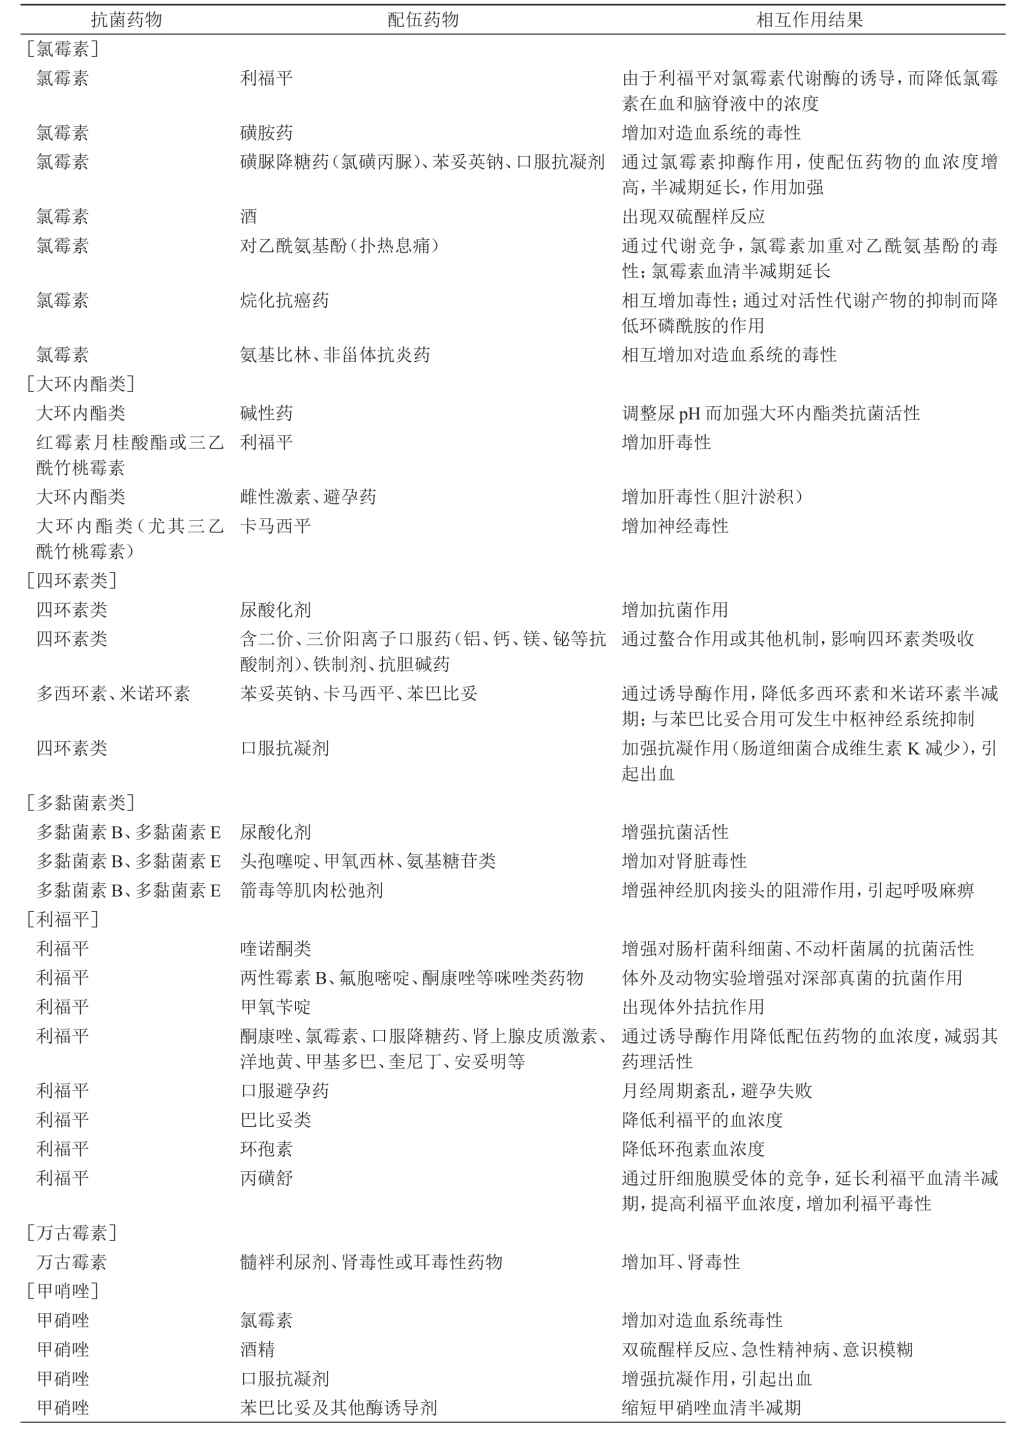
\includegraphics[width=\textwidth,height=\textheight,keepaspectratio]{./images/Image00601.jpg}\\
 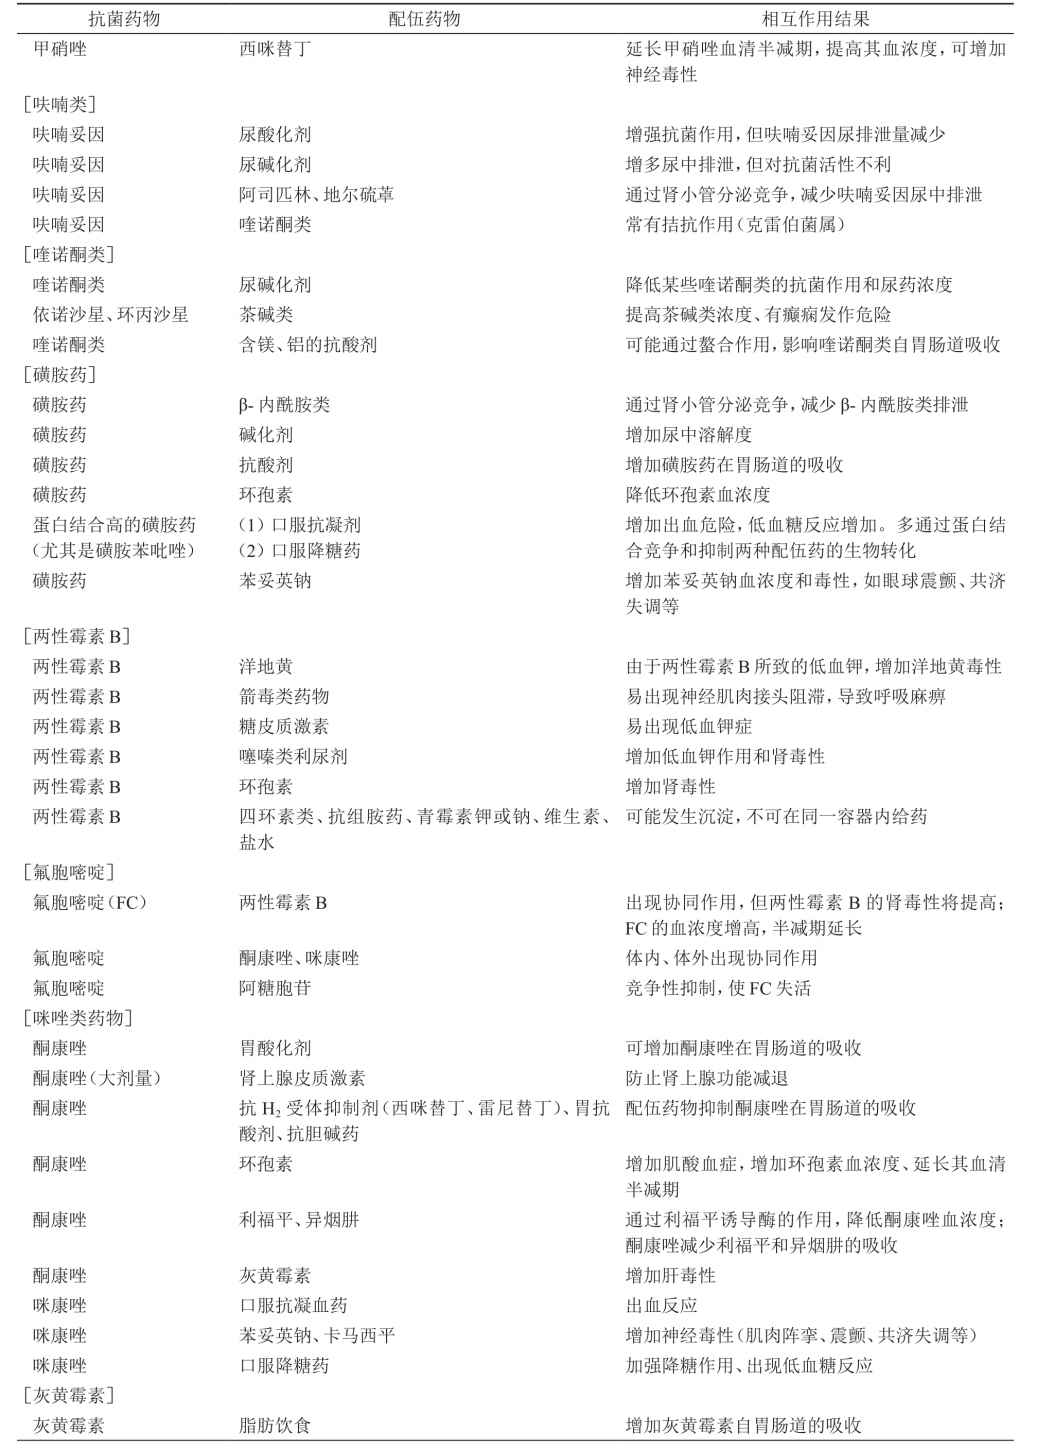
\includegraphics[width=\textwidth,height=\textheight,keepaspectratio]{./images/Image00602.jpg}\\
 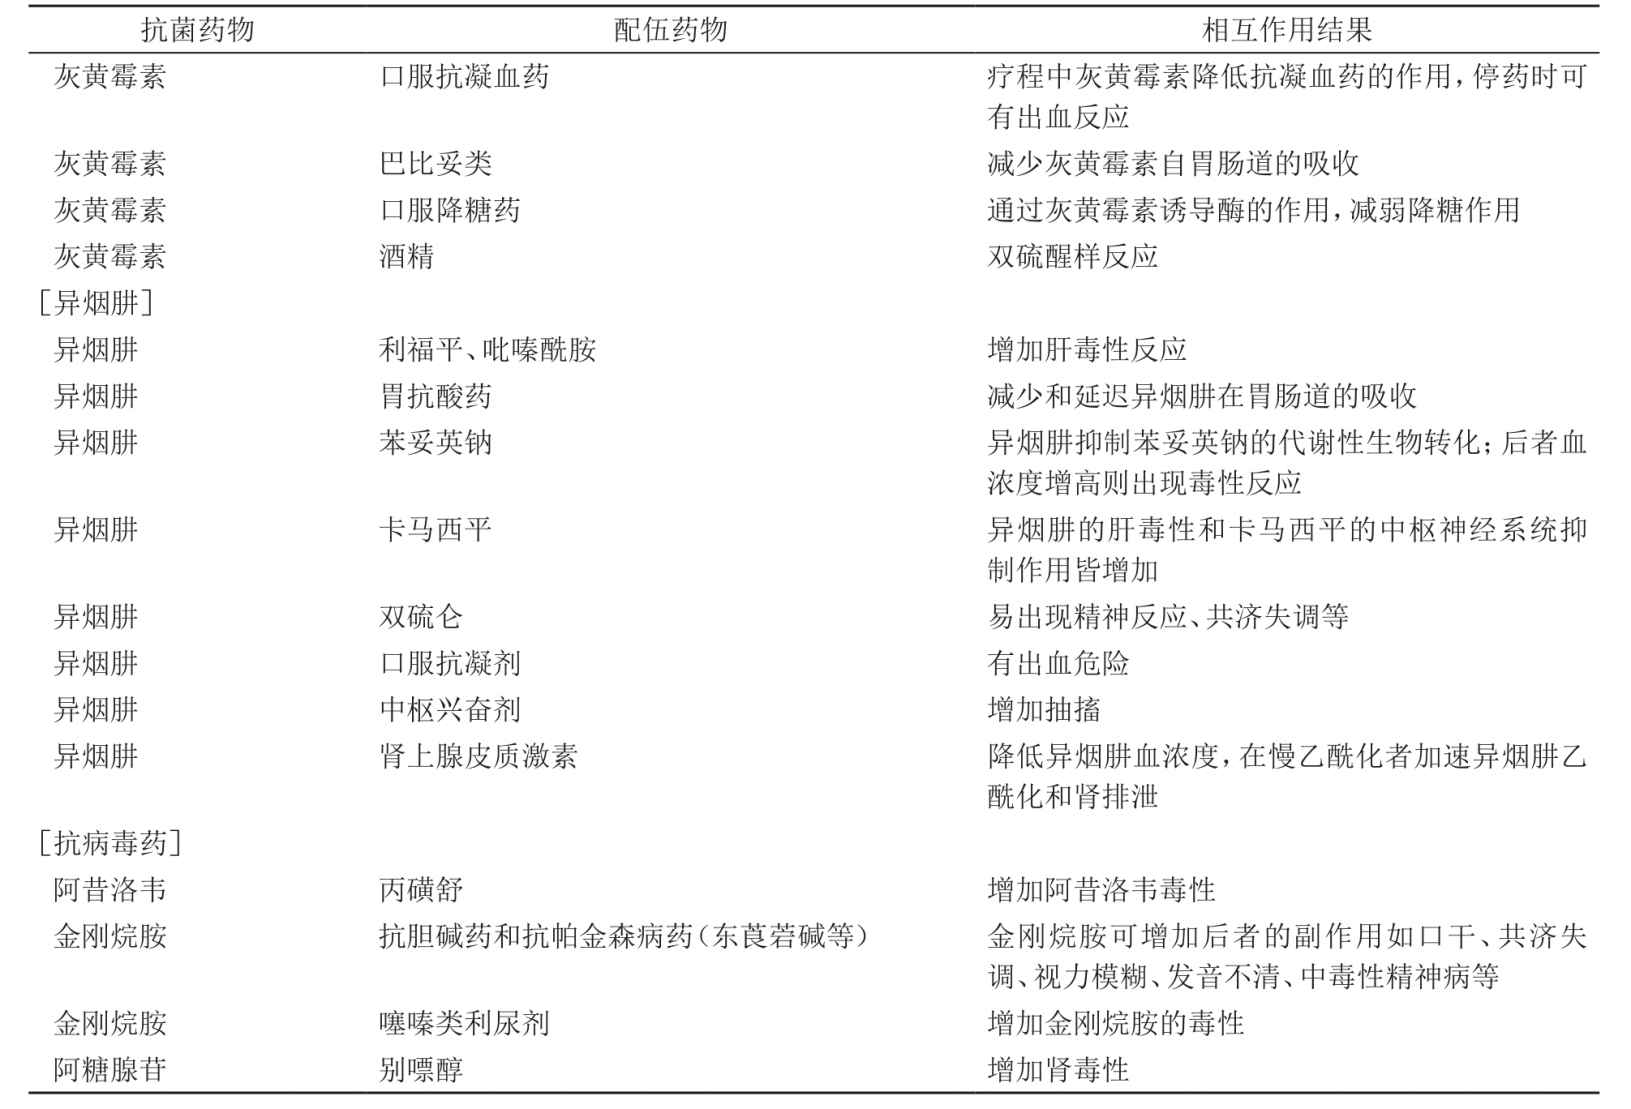
\includegraphics[width=\textwidth,height=\textheight,keepaspectratio]{./images/Image00603.jpg}
 \end{longtable}



\protect\hypertarget{text00436.html}{}{}

\section{抗菌药物的不良反应}

\subsubsection{毒性反应}

药物包括抗菌药物的毒性反应是指药物引起的生理、生化等功能异常和(或)组织、器官等的病理改变,其严重程度每随剂量的增大和疗程延长而增加;其机制可为药物的化学刺激、人体细胞蛋白质合成或酶系功能受阻等,也可因宿主原有的遗传缺陷或病理状态而诱发。毒性反应是抗菌药物所引起的各种不良反应中最常见的一种,主要表现在肾、神经系统、肝、血液、胃肠道、给药局部等。

\hypertarget{text00436.htmlux5cux23CHP17-7-7-1-1}{}
(一) 肾脏

肾是大多数抗菌药物的主要排泄途径
,药物在肾皮质内常有较高浓度积聚,因此肾毒性相当常见。肾小管上皮细胞中积聚的药物浓度远较血液中为高,可因而抑制蛋白质合成、酶系功能、离子交换等,故肾小管病变最为常见;间质性肾炎最可能为一种免疫反应;其他造成肾损害的因素尚有肾血流灌注减少、药物结晶阻塞肾小管或尿路等。

发生肾毒性的抗菌药物主要有:①氨基糖苷类:本类药物直接损伤肾小管上皮细胞,严重时引起肾小管坏死与急性肾衰。庆大霉素较阿米卡星和奈替米星更易引起。②多黏菌素类:均有肾毒性,常用量即可引起。约20\%在用药4天内发生蛋白尿、血尿、尿少等,约2\%出现肾小管坏死。③头孢菌素类:头孢噻啶因肾毒性强已不用,其他第一代头孢菌素如头孢噻吩和头孢唑林在用量较大时也具一定肾毒性,与其他肾毒性药物如氨基糖苷类、强利尿剂等合用时尤宜注意。④青霉素类:甲氧西林主要引起急性间质性肾炎,使用者约10\%~15\%发病,氨苄西林偶也可引起。一般于用药7~10天后发生皮疹、发热、嗜酸性粒细胞增高、血尿等,甚至致进行性肾功能损害。⑤两性霉素B:可致多种肾损害。⑥磺胺药:主要由于药物在肾小管内结晶析出,引起血尿或梗阻性肾病,甚至发生少尿或急性肾衰。还可通过免疫反应引起急性间质性肾炎、肾小球肾炎、坏死性血管炎等。⑦万古霉素:与其他多肽类抗生素(多黏菌素类、杆菌肽等)一样,主要损及肾小管,其肾毒性发生率约为5\%,与庆大霉素合用可增至30\%以上。⑧其他:尚有四环素类、利福平等。

肾毒性(氨基糖苷类、两性霉素B、万古霉素等)的最早症状为蛋白尿和管型尿,继而尿中出现红细胞,并发生尿量改变(增多或减少)、pH改变(大多自酸性转为碱性)、氮质血症、肾功能减退等,其损害程度与剂量及疗程成正比(间质性肾炎除外)。一般于给药后3~6天发生,停药后5天内消失或逐渐恢复。少数患者可出现急性肾衰、尿毒症等。

\hypertarget{text00436.htmlux5cux23CHP17-7-7-1-2}{}
(二) 神经系统

\paragraph{中枢神经系统}

青霉素类尤其是青霉素的全身用药剂量过大和(或)静注速度过快时,可对大脑皮质产生直接刺激作用,出现肌阵挛、惊厥、癫痫、昏迷等严重反应,称为“青霉素脑病”(penicillin
encephalopathy)。一般于用药后24~72小时内出现,可早仅8小时或迟至9天发生。异烟肼、环丝氨酸等的剂量过大可使脑内谷氨酸脱羧酶的活性减低、维生素B\textsubscript{6}
缺乏和γ-氨基丁酸(GABA)的含量减少而导致癫痫。鞘内或脑室内注入青霉素类、氨基糖苷类、多黏菌素B、两性霉素B等,即使为常用量,也可引起一些脑膜刺激征如头痛、颈项轻度强直、呕吐、感觉过敏、背和下肢疼痛、尿频、发热等;当注入量较大时则可发生高热、惊厥、昏迷、尿潴留、呼吸和循环衰竭,甚至导致死亡。

\paragraph{脑神经}

第8对脑神经损害或耳毒性为氨基糖苷类的主要毒性反应之一,与其他耳毒性药物如强利尿剂、水杨酸类、抗癌药(长春新碱等)、砷、汞、奎宁、万古霉素、多黏菌素类等合用时毒性反应将协同加剧,噪声、失水、缺氧、肾功能减退等均系诱发因素,老年人和婴儿尤易发生。耳毒性的发生机制与内耳淋巴液中药物浓度较高有关。氨基糖苷类中对耳蜗毒性较强者为新霉素和卡那霉素,对耳前庭损害较著者为链霉素和庆大霉素。其他抗生素如万古霉素、多黏菌素类、米诺环素、紫霉素、卷曲霉素等也具一定耳毒性,红霉素、氯霉素等偶也可引起。耳蜗损害的先兆表现为耳饱满感、头晕、耳鸣等,也可并无预兆,高频听力每先有减退,继以耳聋。耳前庭损害的表现为眩晕、头痛,急剧动作时可发生恶心、呕吐、伴眼球震颤,严重者可致平衡失调,步态不稳,每一动作停止后似仍在继续进行,向左右转侧有持续滚动感,前俯有倾跌感。大多为暂时性,少数可持续较长时间。

\paragraph{神经肌肉接头处阻滞}

乙酰胆碱(Ach)为神经冲动的传递介质,Ach由神经末梢释放时需有Ca\textsuperscript{2+}
的参与,氨基糖苷类等可与Ca\textsuperscript{2+}
竞争结合部位,从而使Ach的释放受阻,导致神经肌肉接头处受到阻滞。所以,大剂量氨基糖苷类静脉快速注射或手术过程中对接受麻醉剂和(或)肌肉松弛剂者在胸腹腔内应用较大量本类药品,可引起肌肉麻痹,临床表现为四肢软弱、周围血管性血压下降以及心肌抑制症状等,严重者可因呼吸肌麻痹而危及生命。多黏菌素类也可引起同样现象;林可霉素类、四环素类等也偶可发生。

\paragraph{周围神经}

链霉素、庆大霉素、多黏菌素类、异烟肼、硝基呋喃类、乙胺丁醇等可引起周围神经炎,乃与Ca\textsuperscript{2+}
缺乏、维生素B\textsubscript{6}
缺乏、药物直接刺激末梢神经等因素有关。链霉素、多黏菌素类、庆大霉素等注射后可引起口唇及手足麻木,严重者伴头昏、面部和头皮麻木、舌颤等,可能系药物(氨基糖苷类)与Ca\textsuperscript{2+}
螯合所致。异烟肼与乙胺丁醇可因维生素B\textsubscript{6}
缺乏而导致周围神经炎。患者先有趾、足的感觉异常,逐渐波及上肢,进而出现肢体远端肌力减退和腱反射消失。

\hypertarget{text00436.htmlux5cux23CHP17-7-7-1-3}{}
(三) 肝脏

能引起肝脏损害的药物主要有四环素类
、红霉素酯化物、磺胺药、抗结核药物、呋喃唑酮等,其他尚有β-内酰胺类(青霉素类、头孢菌素类等)、两性霉素B等。四环素静脉注射量较大或长期口服时有可能引起急性或亚急性肝细胞脂肪变性,孕妇、长期口服避孕药者、肾肝功能减退者及血浆白蛋白低下者尤易发生,临床表现如急性病毒性肝炎。红霉素的酯化物可引起胆汁淤积性黄疸,临床表现主要有黄疸、瘙痒、上腹痛,可伴发热;恢复迅速,无后遗症。红霉素酯化物中最易引起本病者为红霉素月桂酸盐(俗称“无味红霉素”),其他如红霉素乳糖酸盐偶也可引起。磺胺药引起肝脏损害,可出现类似肝炎的表现,可伴有发热、关节痛、皮疹、嗜酸性粒细胞增多等,严重者可发展为急性或亚急性肝坏死。其他抗菌药物引起的肝损害多表现为血清转氨酶升高。

\hypertarget{text00436.htmlux5cux23CHP17-7-7-1-4}{}
(四) 血液系统

\paragraph{贫血}

氯霉素最为突出,其可引起3种类型贫血:①红细胞生成抑制所致的贫血:当氯霉素血浓度较高,尤其是在较长期使用时,氯霉素分子中的“硝基苯基团”或“苯环对位基团”可损害红细胞的线粒体而抑制其生成;血红素合成酶紧密结合在线粒体内膜上,线粒体受损时其活力明显降低,导致血红蛋白的合成减少。一般在用药期间发生,停药后大多恢复。②再生障碍性贫血(再障):氯霉素是最易引起再障的抗菌药物,与剂量大小无关,发生率虽低,但病死率高于50\%。多见于12岁以下的女性儿童。发生机制可能与氯霉素分子中的硝基苯基团选择性抑制骨髓干细胞、阻止DNA的合成以及骨髓干细胞有遗传性缺陷有关。③葡萄糖-6-磷酸脱氢酶(G-6-PD)缺乏所致的贫血:G-6-PD参与红细胞的无氧糖酵解途径,通过还原型谷胱甘肽而保持红细胞的稳定性。G-6-PD缺乏时红细胞已处于不稳定状态,氯霉素可使还原型谷胱甘肽氧化,因此易于诱发溶血性贫血。

在G-6-PD缺乏时可诱发溶血性贫血的抗菌药物尚有磺胺药、呋喃类等。此外,两性霉素B可与红细胞膜上的固醇结合,使细胞膜的通透性发生改变而发生溶血。β-内酰胺类如青霉素类、头孢菌素类等偶可因附着于红细胞膜上的抗原与相应抗体,或免疫复合物在补体的作用下非特异地吸附在红细胞膜上,并发生作用而引起溶血性贫血。

\paragraph{白细胞与血小板减少}

很多抗菌药物如氯霉素、四环素类、两性霉素B、灰黄霉素等均可引起白细胞和(或)血小板减少,但发生率均较低,停药后很快恢复。其机制可为药物对骨髓幼稚细胞的抑制,或系一种免疫反应。

\paragraph{凝血机制异常}

β-内酰胺类可抑制肠道内产生维生素K的菌群,而维生素K是肝细胞微粒体羧化酶必需的辅助因子,参与凝血酶原前体中谷氨酸的γ-羧化反应,其缺乏将使凝血酶原的合成减少和依赖维生素K的凝血因子Ⅱ、Ⅶ、Ⅸ、Ⅹ等的水平降低。此外,β-内酰胺类尚可阻断ADP诱导血小板凝集的作用。因此,大剂量应用β-内酰胺类(主要为青霉素类和头孢菌素类)后有发生出血如鼻出血、消化道出血(包括大便隐血阳性)等的可能。

\hypertarget{text00436.htmlux5cux23CHP17-7-7-1-5}{}
(五) 胃肠道

大多抗菌药物口服后或注射后胆汁中浓度较高者均可引起一些胃肠道的副作用如恶心、上腹不适、胀气、腹泻等。化学性刺激是胃肠道反应的主要原因,也可是肠道菌群失调的结果,或二者兼而有之。四环素类引起的胃肠道反应最为常见。

\hypertarget{text00436.htmlux5cux23CHP17-7-7-1-6}{}
(六) 其他毒性反应

其他毒性反应尚有:

\paragraph{对牙齿的影响}

四环素类可沉积在牙齿及骨质内,可引起乳齿黄染和牙釉质发育不全。

\paragraph{灰婴综合征}

早产儿和新生儿应用较大剂量氯霉素{[}>
100mg/(kg•d){]}时,常于用药3~4天后出现呕吐、进行性苍白、发绀、循环衰竭、呼吸不规则,患儿可于症状出现后数小时内死亡,及时停药则有迅速恢复的可能。

\paragraph{颅内压增高}

婴幼儿多见,发生于应用四环素类后。停药后症状迅速消失。

\paragraph{不纯制剂的发热反应}

多见于应用两性霉素B的过程中,万古霉素静滴也偶可引起。

\paragraph{其他}

尚有心脏损害、内毒素引起的“治疗休克”等。

\subsubsection{变态反应}

变态反应是应用抗菌药物后的常见不良反应之一,几乎每一抗菌药物均可引起一些变态反应,最多见者为皮疹,其他尚有过敏性休克、血清病型反应、药物热、血管神经性水肿、嗜酸性粒细胞增多症、溶血性贫血、再障、接触性皮炎等。

\paragraph{过敏性休克}

由Ⅰ型变态反应引起。以青霉素最多见,各种途径如注射、口服、点眼、滴鼻、皮试、气溶吸入等均可引起,以注射者最为多见。氨基糖苷类(链霉素、庆大霉素等)也较常见;磺胺药、四环素类、林可霉素类、大环内酯类、氯霉素、利福平等也偶可发生过敏性休克。

\paragraph{药物热}

其潜伏期一般为7~12天,短则仅1天,长者达数周。热型大多为弛张热或稽留热,停药后2~3天内大多可以退热。药物热的特点有:①应用抗菌药物后感染得到控制,体温下降后又再上升;②原来感染所致的发热未被控制,应用抗菌药物后体温反而比未用前为高;③发热或热度增高不能用原有感染解释,而且也无继发感染的证据。患者虽有高热,但其一般情况良好;④某些患者尚伴有其他变态反应如皮疹、嗜酸性粒细胞增多等;⑤停用抗菌药物后热度迅速下降或消退。

\paragraph{皮疹}

每一抗菌药物均可引起皮疹。多于治疗开始后10天左右出现,在以往曾接受同一抗菌药物的患者中,则可于数小时到2天内迅速出现;一般持续5~10天后消退,停药后1~3天内迅速退清。各型皮疹如荨麻疹、斑丘疹、红斑、麻疹样皮疹、猩红热样皮疹、天疱疮样皮疹、湿疹样皮疹、结节样红斑、多形性红斑、紫癜、剥脱性皮炎、大疱表皮松解萎缩性皮炎、渗出性红斑等均有所见,但以荨麻疹、斑丘疹、麻疹样皮疹等多见。在用药过程中,出现皮疹时以及时停药为妥,对有轻型皮疹而必须继续用药者,则宜在相应措施(肾上腺皮质激素、抗组胺药等)的采用下严密观察;若皮疹继续发展,并伴有其他变态反应及发热者应立即停药。

\paragraph{血清病样反应}

属Ⅲ型变态反应,多见于应用青霉素的患者,其症状与血清病基本相同,有发热、关节疼痛、荨麻疹、淋巴结肿大、腹痛、蛋白尿、嗜酸性粒细胞增多等。

\paragraph{血管神经性水肿}

属Ⅲ型变态反应。大多数由青霉素所引起,四环素类、氯霉素、红霉素、链霉素等也偶可引起。

\paragraph{接触性皮炎}

与链霉素、青霉素等抗菌药物经常接触的工作人员有发生接触性皮炎的可能(属Ⅳ型变态反应),一般于接触后3~12个月内发生。表现为皮肤瘙痒、发红、丘疹、眼睑水肿、湿疹等,停止接触后皮炎逐渐消退。

\subsubsection{二重感染}

二重感染也称菌群交替症,是抗菌药物应用过程中出现的新感染。在正常情况下,人体的口腔、呼吸道、肠道、生殖系统等处都有细菌寄生繁殖,这些细菌多数为条件致病菌,少数属致病菌或纯寄生菌。寄殖菌群在互相拮抗制约下维持平衡状态。当较长期应用广谱抗菌药物后,敏感菌群受到抑制而未被抑制者则乘机大量繁殖。此外,原发疾病严重、大手术、应用肾上腺皮质激素和抗代谢药物等均可损害人体的免疫功能,也为细菌入侵和继发感染创造了有利条件。在肠道、呼吸道等部位未被抑制的细菌及外来细菌均可乘虚而入,导致二重感染。二重感染的致病菌主要有革兰阴性杆菌、真菌、葡萄球菌属等,所引起的感染有口腔及消化道感染、肺部感染、尿路感染、败血症等,发生率约2\%~3\%,一般出现于用药后3周内,多见于长期应用广谱抗菌药物者、婴儿、老年人、有严重原发病(如恶性肿瘤、白血病、糖尿病、肝硬化等)者及进行腹部大手术者。

\protect\hypertarget{text00437.html}{}{}

\section{抗菌药物分级管理}

根据抗菌药物的特点、临床疗效、细菌耐药性、不良反应以及当地社会经济状况、药品价格等因素,将抗菌药物分为非限制使用、限制使用与特殊使用三类进行分级管理。

\subsubsection{抗菌药物分级原则}

\paragraph{非限制使用级抗菌药物}

经临床长期应用证明安全、有效,对细菌耐药性影响较小,价格相对较低的抗菌药物。

\paragraph{限制使用级抗菌药物}

与非限制使用级抗菌药物相比较,该类药物在疗效、安全性、对细菌耐药性影响、药品价格等某方面存在局限性,不宜作为非限制级药物使用。

\paragraph{特殊使用级抗菌药物}

具有明显或严重不良反应,不宜随意使用的抗菌药物;需要加以保护以免细菌过快产生耐药而导致严重后果的抗菌药物;新上市不足五年的抗菌药物,其疗效或安全性任何一方面的临床资料尚较少,或并不优于现用药物的;药品价格昂贵的抗菌药物。

2009年3月卫生部办公厅颁布的《关于抗菌药物临床应用管理有关问题的通知》中规定以下药物归属特殊使用级抗菌药物:①第四代头孢菌素:头孢吡肟、头孢匹罗、头孢噻利等;②碳青霉烯类抗菌药物:亚胺培南/西司他丁、美罗培南、帕尼培南/倍他米隆、比阿培南等;③多肽类与其他抗菌药物:万古霉素、去甲万古霉素、替考拉宁、利奈唑胺等;④抗真菌药物:卡泊芬净,米卡芬净,伊曲康唑(口服液、注射剂),伏立康唑(口服剂、注射剂),两性霉素B含脂制剂等。

\subsubsection{抗菌药物分级管理办法}

临床选用抗菌药物应遵循卫生部颁布的《抗菌药物临床应用指导原则》和《抗菌药物临床应用管理办法》,根据感染部位、严重程度、致病菌种类以及细菌耐药情况、患者病理生理特点、药物价格等因素加以综合分析考虑。

1.预防感染、治疗轻度或局部感染应首先选用非限制使用类抗菌药物;严重感染、免疫功能低下者合并感染或病原菌只对限制使用类抗菌药物敏感时,可选用限制使用抗菌药物;特殊使用类抗菌药物的选用应从严控制。

2.二级以上医院应当对本机构执业医师和药师进行抗菌药物使用知识和规范化管理的培训。执业医师经考核合格后取得抗菌药物处方权,药师经考核合格后取得抗菌药物调剂资格。其他医疗机构执业医师、药师由设区的市级卫生行政部门组织相关培训、考核,经考核合格的,授予抗菌药物处方权或调剂资格。

3.临床医师可根据诊断和患者病情开具非限制使用抗菌药物处方。

4.中级及以上专业技术职务任职资格的医师,经培训并考核合格后,方可授予限制使用级抗菌药物处方权。具有高级专业技术职称的医师,经培训和考核合格后,可授予特殊使用级抗菌药物处方权和特殊使用级抗菌药物会诊资格。

5.临床使用特殊使用级抗菌药物
,应当严格掌握用药指征。临床使用特殊使用级抗菌药物应当经抗菌药物管理工作组认定的会诊人员会诊同意后,由具有相应处方权医师开具处方。门诊医师不得开具特殊使用级抗菌药物处方。

特殊使用级抗菌药物会诊人员由具有丰富抗菌药物临床应用经验的感染性疾病科、呼吸科、重症医学科等具有高级专业技术职务任职资格的医师和抗感染专业临床药师担任,资格由抗菌药物管理组负责认定。

6.紧急情况下 ,医师可以越级使用抗菌药物,但仅限于1天用量。

7.下列情况可直接使用限制使用级抗菌药物进行治疗,但当细菌培养及药敏试验证实非限制使用抗菌药物有效时仍应使用非限制使用级抗菌药物:

(1)
严重感染者:如:①败血症、感染性休克;②中枢神经系统感染;③经心肺复苏存活的患者;④脏器穿孔者;⑤感染性心内膜炎;⑥严重的蜂窝组织炎;⑦重度烧伤及其他重症感染者。

(2)
免疫状态低下患者发生感染时:包括:①接受免疫抑制剂治疗;②接受抗癌化学疗法;③外周血WBC计数<
1.0 × 10\textsuperscript{9} /L或中性粒细胞< 0.5 × 10\textsuperscript{9}
/L;④艾滋病患者。

\subsubsection{常用抗菌药物的使用分级(表\ref{tab154-13})}

\begin{table}[htbp]
\centering
\caption{常用抗菌药物使用分级}
\label{tab154-13}
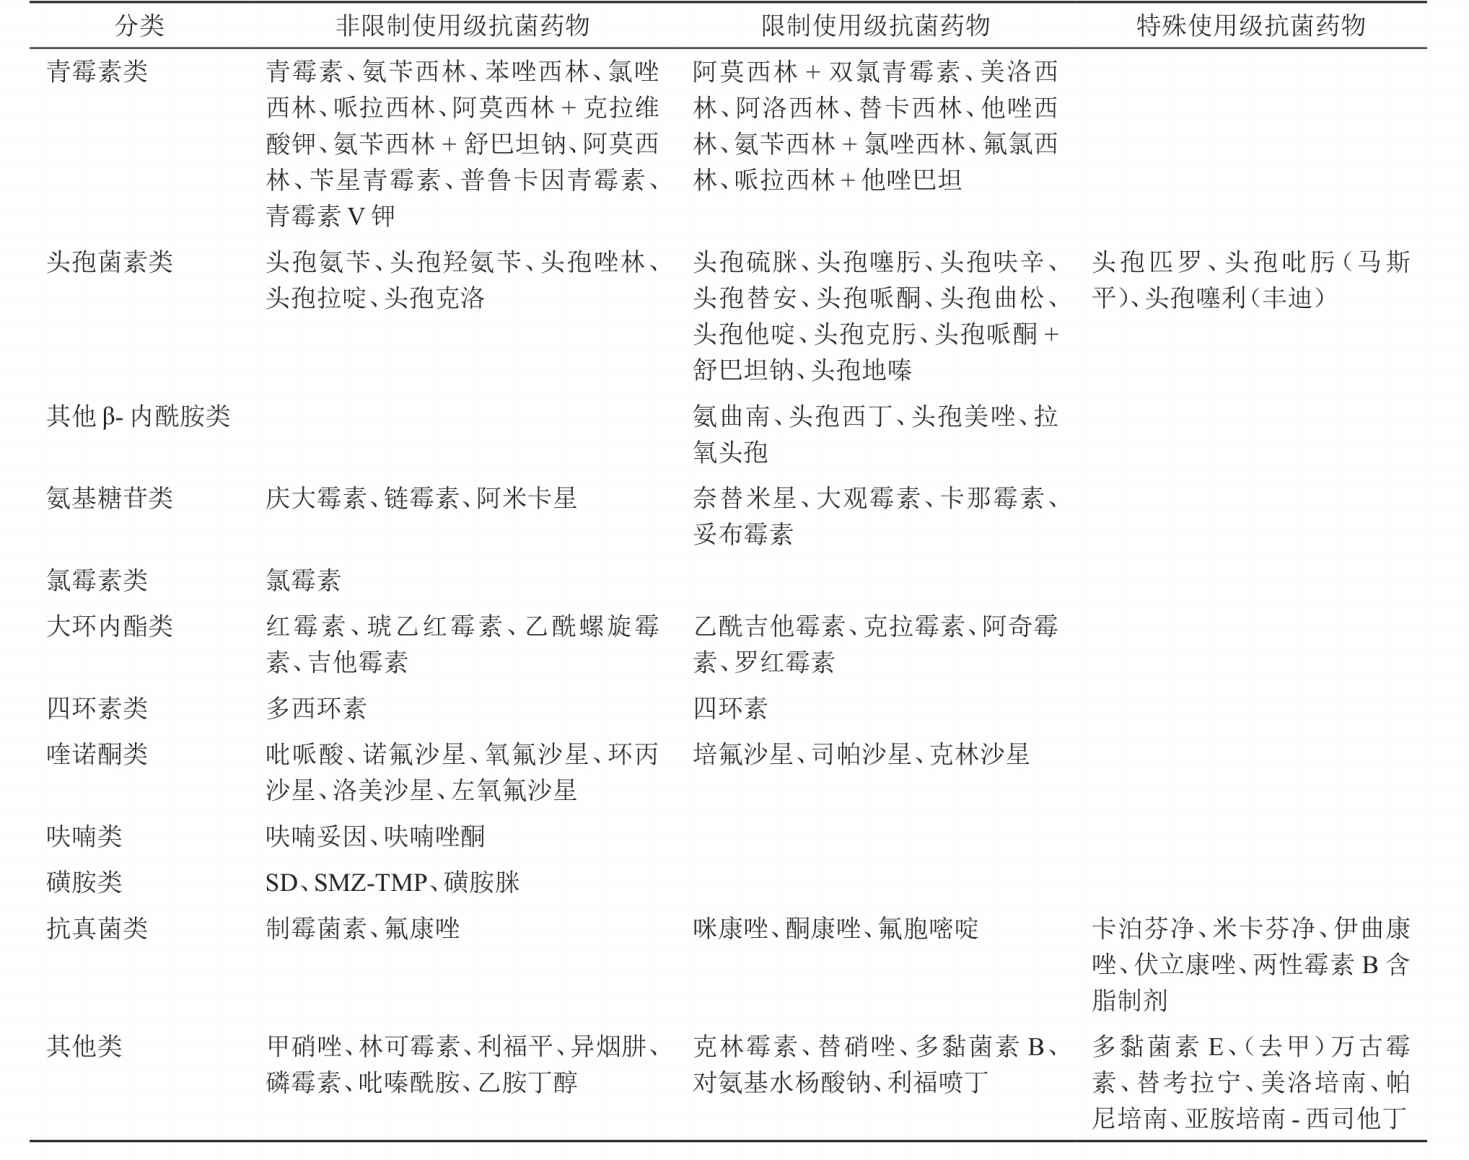
\includegraphics[width=6.78125in,height=5.35417in]{./images/Image00604.jpg}
\end{table}

\protect\hypertarget{text00438.html}{}{}

\chapter{止 血 药}

止血药是能加速血液凝固或降低毛细血管通透性,使出血停止的药物。人体的止血功能是由血管、血小板和凝血系统组成,这三种因素任何一种发生先天性或获得性缺陷即可能发生出血不易止住。但是,也有一些出血不能用这三种因素解释如痔疮出血、食管静脉曲张出血和子宫功能性出血等。它们是由于大血管的畸形、破裂所致,如不采取局部措施仅用止血药不能有效止血。止血药是针对与止血功能有关的三因素研发的,可有效的纠正由于三因素缺陷所造成的止血功能障碍发生的出血。因此,使用止血药时要针对出血原因用药才能奏效。临床上根据止血机制的不同,可将止血药物分为以下几类:①促进凝血因子活性的止血药:如维生素K、去氨加压素(1-去氨基-D-精氨酸加压素,DDAVP,商品名“弥凝”)、重组活化的人凝血因子Ⅶa(rhFⅦa)、注射用血凝酶(立止血)、因子Ⅷ制剂、凝血酶原复合物、鱼精蛋白、血小板浓缩液等;②抗纤维蛋白溶解的止血药:如氨基己酸、氨甲苯酸、氨甲环酸、抑肽酶等;③作用于血管的止血药:如酚磺乙胺、芦丁、卡巴克络、脑垂体后叶素等;④局部止血药:如氧化纤维素、吸收性明胶海绵、凝血酶、云南白药等。临床常用的止血药有:

\subsubsection{促进凝血活性的止血药}

\hypertarget{text00438.htmlux5cux23CHP17-8-1-1}{}
(一) 亚硫酸氢钠甲萘醌(维生素K\textsubscript{3} ,vitamine
K\textsubscript{3} )

\paragraph{药理与应用}

维生素K是一组具有萘醌结构的物质,有K\textsubscript{1}
、K\textsubscript{2} 、K\textsubscript{3} 、K\textsubscript{4}
四种,它们在肝脏微粒体酶系统中是一种重要的辅因子参与肝脏合成依赖维生素K的凝血因子Ⅱ(凝血酶原)、Ⅶ、Ⅸ、Ⅹ,催化这些凝血因子的前体蛋白分子氨基末端谷氨酸残基的γ羧基化,形成可供Ca\textsuperscript{2+}
结合点使它们具有生理活性,缺乏维生素K时肝脏仅合成无凝血活性的上述因子前体蛋白,影响凝血过程使凝血酶原时间延长而发生出血。此时给予维生素K可达到止血作用。本品尚具镇痛作用,其镇痛作用机制可能与阿片受体和内源性阿片样物质介导有关,临床用于胆石症、胆道蛔虫引起的胆绞痛。天然的维生素K\textsubscript{1}
、K\textsubscript{2}
是脂溶性的,其吸收有赖于胆汁的正常分泌;维生素K\textsubscript{3}
是水溶性的,其吸收不依赖于胆汁,口服可直接吸收,也可肌注。吸收后随β脂蛋白转运,在肝内被利用,但常数日才能使凝血酶原恢复至正常水平。临床上维生素K\textsubscript{3}
用于梗阻性黄疸、胆瘘、慢性腹泻、广泛肠切除所致肠吸收功能不良患者,早产儿、新生儿低凝血酶原血症,香豆素类或水杨酸类过量以及其他原因所致凝血酶原过低等引起的出血;亦可用于预防长期口服广谱抗生素类药物引起的维生素K缺乏症。临床还常用维生素K\textsubscript{3}
解救杀鼠药“敌鼠钠”中毒,此时应用大剂量或输注凝血酶原复合物。

\paragraph{用法}

①止血:口服:一次2~4mg,一日6~24mg;肌注,每次4mg,每天2~3次;防止新生儿出血,可在产前一周给孕妇肌注,每日2~4mg。②胆绞痛:肌注,每次8~16mg。

\paragraph{制剂}

注射液:每支2mg(1ml)、4mg(1ml)。

\paragraph{注意事项}

①可致恶心、呕吐等胃肠道反应;②较大剂量可致新生儿、早产儿溶血性贫血、高胆红素血症及黄疸。在红细胞6-磷酸脱氢酶缺乏症患者可诱发急性溶血性贫血;③可致肝损害。肝功能不良患者可改用维生素K\textsubscript{1}
,肝硬化或晚期肝病患者出血,使用本品无效。④禁用于对本品过敏者及妊娠晚期妇女。

\hypertarget{text00438.htmlux5cux23CHP17-8-1-2}{}
(二) 醋酸去氨加压素(1-去氨基-精氨酸加压素,DDAVP)

\paragraph{药理与应用}

本品能促使血管性血友病因子(von Willebrand
factor,vWF)从血管内皮细胞等部位释放,是多聚蛋白,具有促进血小板黏附和保护因子Ⅷ:C的作用,用于Ⅰ型血管性血友病和轻型血友病A患者,可控制轻度出血发作,也可用于拔牙或手术过程中预防出血。本品对需要采取紧急措施的尿毒症出血患者可有暂时止血作用;也可暂时纠正慢性肝病或血小板功能异常的止血缺陷。本品可促使纤溶酶原释放,因此在应用本品时合用抗纤溶药直至伤口愈合或出血停止。

\paragraph{用法}

每次0.3~0.5μg/kg加入生理盐水20~30ml中,于15~20分钟内静脉滴注,间隔12~24小时重复注射,2~5次为一疗程。鼻内滴入剂量要大,每次10~20μg,每天1~2次,但不能大于30μg或0.5μg/kg,疗效比静脉注射差。

\paragraph{剂型}

注射剂:4μg/ml;滴鼻剂:100μg/ml。

\paragraph{注意事项}

不同个体对本品存在明显差异,重复应用会产生耐受性。不良反应有头痛、恶心、呕吐或肠道痉挛,注射部位疼痛,脸面潮红,偶有发热、皮疹或呼吸困难等变态反应。因本品具有抗利尿作用,可引起水潴留,因此用本品时必须注意体液平衡。以免发生水中毒和低钠血症。本品可引起血压轻度升高,心率加快,因而高血压和冠心病患者慎用。

\hypertarget{text00438.htmlux5cux23CHP17-8-1-3}{}
(三) 重组活化凝血因子 Ⅶ(rhFⅦa)

重组活化的人凝血因子Ⅶ(rhFⅦa)系因子Ⅶa-组织因子复合物,除激活因子Ⅹ外还可激活因子Ⅸ,因子Ⅶa在内源性途径和外源性途径的激活中都发挥关键作用。rhFⅦa对先天性因子Ⅶ缺乏、产生抑制物的血友病A和B、血小板减少等都有效。静脉注射35~70μg/kg每2~3小时一次,连用2~3次。

\hypertarget{text00438.htmlux5cux23CHP17-8-1-4}{}
(四)
注射用血凝酶(hemocoagulase,蛇凝血素酶,其商品名为立止血,Reptilase)

\paragraph{药理与应用}

本品具有类凝血酶样作用及类凝血激酶样作用。其凝血酶样作用能促进出血部位(血管破损部位)的血小板聚集,释放一系列凝血因子,其中包括血小板因子3(PF\textsubscript{3}
),能促进纤维蛋白原降解生成纤维蛋白Ⅰ单体,进而交联聚合成难溶性纤维蛋白,促进在出血部位的血栓形成和止血。其类凝血激酶样作用是由于释放的PF\textsubscript{3}
引起,就像血液中的凝血激酶依靠PF\textsubscript{3}
激活那样,凝血激酶被激活后,可加速凝血酶的生成,因而促进凝血过程。本品在完整无损的血管内无促进血小板聚集作用,它不激活血管内纤维蛋白稳定因子(因子Ⅻ),因此,它促进生成的纤维蛋白Ⅰ单体所形成的复合物,易在体内被降解而不致引起DIC。静脉注射5~10分钟起效,止血效应持续24小时;肌内注射或皮下注射20分钟后起效,持续48小时。其代谢产物随尿排出体外。立止血用于临床各科室的出血及出血性疾病;也用于手术前给药,减少出血倾向,避免手术部位等手术后出血。

\paragraph{制剂和用法}

注射液:每支含1kU,紧急情况下,立即静注1~2kU,同时肌注1kU;手术前1小时,肌注1kU,或手术前15分钟,静注1kU。手术后每日肌注1kU,一日总量不超过8kU,一般用药不超过3天。

\paragraph{注意事项}

①本品无明显副作用,但为安全起见,不可用于血栓患者。②DIC导致的出血时禁用本品。③妊娠初3个月的孕妇慎用。④治疗新生儿出血,宜与维生素K合用。

\hypertarget{text00438.htmlux5cux23CHP17-8-1-5}{}
(五) 鱼精蛋白(protamine,硫酸鱼精蛋白)

\paragraph{药理与应用}

本品能与肝素结合,使其失去抗凝血能力。临床上用于因注射肝素过量而引起的出血,以及自发性出血如咯血等。

\paragraph{用法}

①抗肝素过量:静注,用量与所用肝素量(最末1次)相当(本品1mg可中和肝素100U),但一般不超过50mg;②抗自发性出血:静滴:5~8mg/(kg•d),分2次用(间隔6小时),加入300~500ml
0.9\%氯化钠注射液中静滴。连用不超过3天。

\paragraph{制剂}

注射液:50mg(5ml),100mg(10ml)。

\paragraph{注意事项}

①静注鱼精蛋白有可能引起血压骤然下降、心搏徐缓、呼吸困难,或一过性潮红等不良反应;也曾有发生变态反应,形成呼吸窘迫等。因此,静注速度应缓慢,10分钟的用量不超过50mg,同时最好备有抢救休克的药物与设备。②用量过量可引起出血,尤其是口服抗凝血药或凝血酶原低下的患者更应注意。③对鱼有过敏史的患者忌用。

\hypertarget{text00438.htmlux5cux23CHP17-8-1-6}{}
(六) 人凝血因子 Ⅷ(human coagulation factor Ⅷ,抗甲种血友病因子)

\paragraph{药理与应用}

本品是一种大分子量的糖蛋白复合物,是由占99\%的血管性血友病因子(vWF)和只占1\%的因子Ⅷ促凝活性(FⅧc)两部分组成。vWF可与血小板膜糖蛋白和内皮胶原蛋白结合,起中间桥联作用,尚有保护FⅧc活性,防止FⅧc的降解作用。FⅧc参与内源凝血途径的凝血反应。用于纠正和预防凝血因子Ⅷ缺乏或因患获得性因子Ⅷ抑制物增多症而引起的出血。主要用于治疗甲型血友病。

\paragraph{用法与用量}

静脉滴注。①轻度关节出血:一次8~10U/kg,每天1~2次,连用1~4天。使FⅧc提高到正常水平的15\%~20\%。②中度关节、肌肉出血:一次15U/kg,每天2次,连用3~7天。使FⅧc提高到正常水平的30\%。③大出血或严重外伤而无出血证据:一次25U/kg,每天2次,至少用7天。使FⅧc提高到正常水平的50\%。④外科手术或严重外伤伴出血:40~50U/kg于术前1小时开始输注,使FⅧc提高到正常水平的80\%~100\%;随后使FⅧc水平维持在正常水平的30\%~60\%,约10~14天,或按下列公式计算:一次所需FⅧc
=体重(kg)×要求增加的FⅧc的浓度(\%)×
0.5。⑤预防出血:体重≥50kg,500U/d;<
50kg,250U/d。使FⅧc水平达到正常水平的5\%~10\%。⑥抗FⅧc抗体生成伴出血:首剂5000~10
000U/h,维持量300~1000U/h,使体内FⅧc水平维持在30~50U/ml,如联合应用血浆置换术,宜追加本品40U/kg,以增强疗效。

\paragraph{制剂}

人凝血因子Ⅷ:每瓶100U;200U;250U;300U;400U;500U;750U;1000U。

\paragraph{注意事项}

①应单独输注,不可与其他药物合用。②大量输注本品可产生溶血反应(抗A、抗B红细胞凝集素)或超容量性心衰,一日输注超过20U/kg时可出现肺水肿。尚可有高凝血因子Ⅰ血症或血栓形成。③可能出现寒战、发热、荨麻疹、恶心、眼睑水肿及呼吸困难等过敏反应,甚至过敏性休克。因此,对本品过敏者禁用。④滴注速度需个体化,一般约2~4ml/min,药液应在1小时内输完。⑤对乙型血友病(FⅨ缺乏)及丙型血友病(FⅪ缺乏)无效。

\subsubsection{抗纤溶药}

\hypertarget{text00438.htmlux5cux23CHP17-8-2-1}{}
(一) 氨基己酸(aminocaproic acid,6-氨基己酸,EACA)

\paragraph{药理与应用}

能抑制纤维蛋白溶酶原的激活因子,使纤维蛋白溶酶原不能激活为纤维蛋白溶酶,从而抑制纤维蛋白的溶解,产生止血作用。高浓度时,本品对纤维蛋白溶酶还有直接抑制作用,对于纤维蛋白溶酶活性增高所致的出血症有良好疗效。口服吸收较完全,生物利用度80\%,2小时左右血药浓度达峰值,有效血浓度为13μg/ml。大部分以原形经尿排泄。临床上用于纤溶性出血,如脑、肺、子宫、前列腺、肾上腺、甲状腺等外伤或手术出血。术中早期用药或术前用药,可减少手术中渗血,并减少输血量。亦用于肺出血、肝硬化出血及上消化道出血。

\paragraph{用法}

静滴:初用量4~6g,以5\%~10\%葡萄糖或生理盐水100ml稀释,15~30分钟内滴完,维持量为1g/h,维持时间依病情而定,一般每日量不超过20g,可连用3~4天。口服:成人每次2g,小儿0.1g/kg,每日3~4次,依病情服用7~10天或更久。

\paragraph{制剂}

注射液:每支1g(10ml),2g(10ml);片剂:每片0.5g。

\paragraph{注意事项}

①偶有腹泻、腹部不适、结膜充血、鼻塞、皮疹、低血压、呕吐、胃灼热感及尿多等反应;②本品排泄较快,须持续给药,否则其血浆有效浓度迅速降低;③本品不能阻止小动脉出血;④本品从肾脏排泄,且能抑制尿激酶,可引起血凝块而形成尿路阻塞,故泌尿道手术后,血尿的患者慎用;⑤静脉给药过快可见低血压、心律失常,不可静脉注射给药;⑥禁用于对本品过敏者、DIC的高凝期患者、有血栓形成倾向或有血管栓塞性疾病史者;注射用制剂禁用于早产儿。

\hypertarget{text00438.htmlux5cux23CHP17-8-2-2}{}
(二) 氨甲苯酸(P-aminomethyl benzoic
acid,PAMBA,止血芳酸,对羧基苄胺,抗血纤溶芳酸)

\paragraph{药理与应用}

本品作用机制与氨基己酸相同,但其作用较之强4~5倍。口服易吸收,生物利用度为70\%,服后3小时血药浓度达峰值,静脉注射后,有效血浓度可维持3~5小时。经肾排泄,t\textsubscript{1/2}
为60分钟。毒性较低,不易生成血栓。适用于纤维蛋白溶解过程亢进所致出血,如肺、肝、胰、前列腺、甲状腺、肾上腺等手术时的异常出血,妇产科和产后出血以及肺结核咯血或痰中带血、血尿、前列腺肥大出血、上消化道出血等,对一般慢性渗血效果较显著,但对癌症出血以及创伤出血无止血作用。此外,尚可用于链激酶或尿激酶过量引起的出血。

\paragraph{用法}

静注:每次0.1~0.3g,用5\%葡萄糖或生理盐水10~20ml稀释后缓慢静注,或加入液体中缓慢静滴,一日最大用量为0.6g;儿童每次0.1g。口服:每次0.25~0.5g,每日3次。

\paragraph{制剂}

注射液:每支0.05g(5ml),0.1g(10ml);片剂:每片0.125g,0.25g。

\paragraph{注意事项}

①用量过大可促进血栓形成,对有血栓形成倾向或有血栓栓塞病史者禁用或慎用。②本品可致继发性肾盂和输尿管凝血,故血友病患者发生血尿时或肾功能不全者慎用。③不单独用于DIC所继发的纤溶性出血,必要时,在肝素化的基础上应用。

\hypertarget{text00438.htmlux5cux23CHP17-8-2-3}{}
(三) 氨甲环酸(tranexamic acid,止血环酸,凝血酸, AMCHA)

\paragraph{药理与应用}

作用与氨甲苯酸相似,但较强。用于各种出血性疾病、手术时异常出血等。

\paragraph{用法}

口服:每次1.0~1.5g,2~6g/d;静脉应用:每次0.25~0.5g,0.75~2.0g/d,静注以25\%葡萄糖液稀释,静滴以5\%~10\%葡萄糖液稀释。

\paragraph{制剂}

片剂:每片0.125g,0.25g;注射液:每支0.1g
(2ml),0.25g(5ml),0.5g(5ml),1.0g(10ml)。

\paragraph{注意事项}

可有头痛、头晕、恶心、呕吐、胸闷等反应。

\subsubsection{血管止血药}

\hypertarget{text00438.htmlux5cux23CHP17-8-3-1}{}
(一) 酚磺乙胺(etamsylate,止血敏,止血定,羟苯磺乙胺,dicynone)

\paragraph{药理与应用}

本品能增加血液中血小板数量,增强其聚集性和黏附性,促使血小板释放凝血活性物质,缩短凝血时间,加速血块收缩。还可增强毛细血管抵抗力,降低毛细血管通透性,减少血液渗出。止血作用迅速,静注后1小时作用达高峰,作用维持4~6小时。口服也易吸收。适用于预防和治疗外科手术出血过多,血小板减少性紫癜或过敏性紫癜以及其他原因引起的出血,如脑出血、肠道出血、泌尿道出血、眼底出血、齿龈出血、鼻出血等。可与其他类型止血药如氨甲苯酸、维生素K并用。

\paragraph{用法}

①预防手术出血:术前15~30分钟静注或肌注0.25~0.5g,必要时2小时后再注射0.25g,一日0.5~1.5g。②治疗出血:成人口服每次0.5~1.0g,儿童每次10mg/kg,每日3次。肌肉或静注:每次0.25~0.75g,每天2~3次,或加入液体中静滴。必要时依病情增加剂量。

\paragraph{制剂}

注射液:每支0.25g(2ml),0.5g(5ml),1.0g
(5ml);片剂:每片0.25g,0.5g。

\paragraph{注意事项}

本品毒副作用较小,偶见过敏反应。有报道静脉注射时曾发生过敏性休克。本品最好单独注射,不宜与其他药物或碱性药液配伍,不可与氨基己酸混合注射。

\hypertarget{text00438.htmlux5cux23CHP17-8-3-2}{}
(二)
卡巴克洛(肾上腺色腙,carbazochrome,安络血,安特诺新,adrenobazone)

\paragraph{药理与应用}

本品为肾上腺素氧化产物肾上腺色素(adrenochrome)的缩氨脲水杨酸钠盐。能增强毛细血管对损伤的抵抗力,降低毛细血管的通透性,促进受损毛细血管端回缩而止血。主要用于毛细血管通透性增加所致的出血,如特发性紫癜、视网膜出血、慢性肺出血、胃肠出血、咯血、鼻出血、血尿、痔出血、子宫出血等。对大量出血和动脉出血疗效较差。

\paragraph{用法}

口服:成人每次2.5~5mg,每日3次;肌注:每次5~10mg。亦可静注。

\paragraph{制剂}

片剂:每片2.5mg,5mg;注射液:每支5mg (1ml),10mg(2ml)。

\paragraph{注意事项}

长期应用,可诱发癫痫及精神错乱等,有癫痫史及精神病史者慎用。对泌尿道或脑出血者应慎用。

\subsubsection{局部止血药}

\hypertarget{text00438.htmlux5cux23CHP17-8-4-1}{}
(一) 凝血酶(thrombin)

\paragraph{药理与应用}

本品是从人或动物血提取、精制而得的凝血酶无菌制剂。能直接作用于血液中的纤维蛋白原,促使转变为纤维蛋白,加速血液的凝固,达到止血目的。还有促进上皮细胞的有丝分裂而加速创伤愈合的作用。可用于通常结扎止血困难的小血管、毛细血管以及实质性脏器出血的止血。临床上用于外伤、手术、口腔、耳鼻喉、泌尿、妇产科以及消化道等部位的止血。

\paragraph{用法}

①局部止血:用无菌生理盐水溶解成每毫升含凝血酶50~1000U,喷雾或灌注于创面,或以明胶海绵、纱条黏附本品后贴附于创面;也可直接撒布本品于创面。②消化道止血:用生理盐水或牛奶(温度不超过37℃)溶解本品成每毫升含50~500U,可口服或灌注,每次用量为500~2000U,每1~6小时用1次。根据出血部位和程度,可适当增减浓度及使用次数。

\paragraph{制剂}

冻干粉剂,每瓶含本品200U、500U、1000U、2000U和5000U等5种规格。

\paragraph{注意事项}

①本品严禁作血管内、肌肉或皮下注射,否则可导致血栓、局部坏死,而危及生命。②若出现过敏反应,应立即停药。③使用时要避免加温、酸、碱或重金属盐类,否则可使本品活力下降而失效。

\hypertarget{text00438.htmlux5cux23CHP17-8-4-2}{}
(二) 氧化纤维素(cellulose oxide)

本品为局部止血药,纤维素中的羧基与血浆中的Ca\textsuperscript{2+}
形成交联键,呈凝胶状血块堵塞破损血管而止血。用于外科不能缝合或结扎的中度出血。用法是将本品贴敷于出血处。本品在体内2~7日逐渐被吸收,6周后完全吸收。

\hypertarget{text00438.htmlux5cux23CHP17-8-4-3}{}
(三) 纤维蛋白胶

纤维蛋白原和凝血酶
,钙离子溶液在出血区混合,形成纤维蛋白膜产生止血作用。适用于外科手术中的止血;在内镜的协助下,可施行腔管内止血(胃及食管等)。

\protect\hypertarget{text00439.html}{}{}

\chapter{镇 痛 药}

镇痛药(analgesic)主要作用于中枢神经系统。在镇痛剂量时可选择性地减轻或缓解疼痛,但并不影响意识、触觉、听觉等其他感觉,同时因疼痛引起的精神紧张、烦躁不安等不愉快情绪也可得到缓解,从而使疼痛易于耐受。大多数镇痛药属于阿片类生物碱,如吗啡及可待因等,也有一些是其同类人工合成品,如哌替啶、美沙酮、喷他佐辛等。本类药物的镇痛作用强大,多用于剧烈疼痛。多数镇痛药连续应用可致成瘾,故亦称成瘾性镇痛药,不宜长期应用。大多数镇痛药对呼吸中枢有抑制作用,中毒剂量时可因呼吸被抑制而死亡。本类药物多通过激动阿片受体而产生镇痛和呼吸抑制效应,其中吗啡、可待因、哌替啶、美沙酮、芬太尼和二氢埃托啡等是阿片受体的完全激动剂,喷他佐辛、布托啡诺、丁丙诺啡和纳布啡等是阿片受体的部分激动剂。纳洛酮是阿片受体拮抗剂,可对抗吗啡的镇痛作用和呼吸抑制作用。

临床上常用的镇痛药有:

\subsubsection{吗啡(morphine)}

\paragraph{药理与应用}

本品为阿片受体激动剂。其药理作用有:

\hypertarget{text00439.htmlux5cux23CHP17-9-1-1-1}{}
(1) 中枢神经系统:

吗啡有强力的镇痛作用,对一切疼痛均有效。成瘾性强。在镇痛的同时有明显镇静作用,能产生欣快感,可改善疼痛患者的紧张情绪。可抑制呼吸中枢,降低呼吸中枢对CO\textsubscript{2}
的敏感性,减慢呼吸频率,也能降低肺潮气量。对呼吸的抑制程度与使用吗啡的剂量平行,过大剂量可致呼吸衰竭而死亡。吗啡可抑制延髓的咳嗽中枢,产生镇咳作用,但因其成瘾性强而不用于临床。吗啡也能兴奋延髓催吐化学感受区,引起呕吐或恶心。此外,尚有缩瞳作用,吗啡中毒时,瞳孔极度缩小。

\hypertarget{text00439.htmlux5cux23CHP17-9-1-1-2}{}
(2) 心血管系统:

可促进内源性组胺释放而使外周血管扩张、血压下降,大剂量则出现心动过缓;使脑血管扩张,颅压增高。

\hypertarget{text00439.htmlux5cux23CHP17-9-1-1-3}{}
(3) 平滑肌:

吗啡可使消化道平滑肌兴奋和便意迟钝,而致便秘;并能使胆道、输尿管、支气管平滑肌张力增加。

临床应用于:①镇痛:仅用于创伤、手术、烧伤等引起的剧痛;②急性心肌梗死;③心源性哮喘;④麻醉前给药。

吗啡可由胃肠道黏膜、鼻黏膜及肺等吸收,皮下及肌内注射吸收均迅速。吸收后可迅速分布于各种组织。半衰期约1小时,1次给药镇痛作用持续4~6小时。主要在肝脏代谢,经肾排泄,可通过胎盘,小量经乳腺及胆汁排出。

\paragraph{用法}

皮下注射或口服,每次5~10mg,每天1~3次。极量:皮下注射,每次20mg,60mg/d;口服每次30mg,100mg/d。

\paragraph{制剂}

注射液:每支5mg(0.5ml),10mg(1ml);片剂:每片5mg,10mg。

吗啡控释片(美施康定,路泰,美菲康)可使药物恒定释放,在达稳态时血药浓度波动小,作用时间可持续12小时。主要用于缓解癌症疼痛和其他各种剧烈疼痛。制剂有每片10mg;30mg;60mg。宜从小剂量开始。

\paragraph{注意事项}

①可引起眩晕、呕吐、便秘、排尿困难等副作用。连续使用容易成瘾,需慎用。②因可经乳腺排出及分布至胎盘,可抑制新生儿及婴儿呼吸,故婴儿及哺乳妇女忌用,临产妇女禁用。③慢性阻塞性肺疾患、甲状腺功能不足(黏液性水肿)、颅内高压、颅脑损伤等禁用;肝功能减退者、急性左心衰竭晚期并出现呼吸衰竭时忌用。④胆绞痛、肾绞痛需与阿托品合用。⑤在疼痛原因未明确前,忌用本品,以防掩盖症状,贻误诊治。⑥急性吗啡中毒的症状有昏迷、呼吸减慢、瞳孔缩小至针尖样,进而可致呼吸麻痹、体温下降。可采用吸氧、人工呼吸、注射对抗药纳洛酮、烯丙吗啡或尼可刹米等。

\subsubsection{哌替啶(pethidine,度冷丁,dolantin,唛啶,地美露,demerol)}

\paragraph{药理与应用}

本品作用及机制与吗啡相似,亦为阿片受体激动剂。镇痛作用相当于吗啡的1/10~1/8,持续时间2~4小时。能短时提高胃肠道括约肌及平滑肌的张力,但不致引起便秘。增加胆道、支气管平滑肌张力的作用较弱,能使胆总管括约肌痉挛。对呼吸有抑制作用。镇静、镇咳作用较弱。能增强巴比妥类的催眠作用。临床应用于:①各种剧痛,如创伤、烧伤、烫伤、术后疼痛等;②心源性哮喘;③麻醉前给药;④内脏剧烈绞痛(胆绞痛、肾绞痛需与阿托品合用);⑤与氯丙嗪、异丙嗪等合用进行人工冬眠。

\paragraph{用法}

①口服:每次50~100mg;极量:每次200mg,600mg/d。②皮下注射或肌注:每次25~100mg,极量:每次150mg,600mg/d。两次用药间隔不宜少于4小时。③静注:成人以每次0.3mg/kg为限。

\paragraph{制剂}

片剂:每片25mg,50mg。注射液:每支50mg (1ml),100mg(2ml)。

\paragraph{注意事项}

①成瘾性比吗啡轻,但连续应用亦成瘾。②副作用有头昏、头痛、出汗、口干、恶心、呕吐等;过量可致瞳孔散大、惊厥、心动过速、幻觉、血压下降、呼吸抑制、昏迷等。③不宜皮下注射,因对局部有刺激性。④儿童慎用。1岁以内小儿一般不应静注本品或行人工冬眠。⑤分娩前2~4小时内不用。⑥不宜与异丙嗪多次合用,否则可导致呼吸抑制,引起休克等不良反应。⑦其他注意事项及禁忌同吗啡。

\subsubsection{美沙酮(methadone,美散痛,phenadon)}

\paragraph{药理与应用}

为阿片受体激动剂。镇痛效力与吗啡相等或略强,止痛效果好。口服有效,服药后5~30分钟产生镇痛作用,维持4~6小时或更长。镇静作用则较轻微,但重复给药仍可引起明显的镇静作用。对呼吸中枢也有明显抑制作用。在肝脏中广泛代谢,主要由尿排泄。临床上适用于创伤性、癌症剧痛及外科手术后镇痛。也用于阿片、吗啡及海洛因成瘾者的脱毒治疗。

\paragraph{用法}

①口服:成人5~10mg/次,每天3次;儿童0.7mg/(kg•d),分4~6次服。②肌注或皮下注射:每次2.5~5mg,1天10~15mg。三角肌注射血浆峰值高,作用出现快。极量:1次10mg,1天20mg。

\paragraph{制剂}

片剂:每片2.5mg,7.5mg;10mg;注射液:每支5mg(1ml),7.5mg(2ml)。

\paragraph{注意事项}

①副作用有头痛、眩晕、恶心、出汗、嗜睡等,但较轻。成瘾性较小,但久用也能成瘾,应予警惕。少数病例用量过大时引起失明、下肢瘫痪。②对本品过敏者、呼吸功能不全者、中毒性腹泻患者、妊娠和分娩期妇女、婴幼儿禁用。③不宜作静脉注射。

\subsubsection{芬太尼(fentanyl)}

\paragraph{药理与应用}

本品为阿片受体激动剂,属强效麻醉性镇痛药。药理作用与吗啡类似,镇痛作用较之强80倍。镇痛作用产生快,但持续时间较短,副作用比吗啡小。适用于各种疼痛及外科、妇科等手术后和手术过程中的镇痛;也用于防止或减轻手术后出现的谵妄;还可与麻醉药合用,作为麻醉辅助用药;与氟哌利多配伍制成“安定镇痛剂”,用于大面积换药及进行小手术的镇痛。

\paragraph{用法}

①麻醉前给药:0.05~0.1mg,于手术前30~60分钟肌注。②诱导麻醉:静注0.05~0.1mg,间隔2~3分钟重复注射,直至达到要求;危重患者,年幼及年老患者的用量减少至0.025~0.05mg。③维持麻醉:当患者出现苏醒状时,静注或肌注0.025~0.05mg。④一般镇痛或术后镇痛:肌注0.05~0.1mg。可控制手术后疼痛、烦躁和呼吸急迫,必要时可于1~2小时后重复给药。⑤贴片:每3天用1贴,贴于锁骨下胸部皮肤。

\paragraph{制剂}

注射液:每支0.1mg(2ml)。复方芬太尼注射液:每ml含芬太尼0.1mg,异丙嗪25mg。贴片(多瑞吉):每小时可释放芬太尼25μg、50μg、75μg、100μg。

\paragraph{注意事项}

①个别病例可出现眩晕、恶心、呕吐、胆道括约肌痉挛的副作用,约1小时后,自行缓解。还可引起视觉模糊、发痒和欣快感,但不明显。②静注时可引起胸壁肌肉强直,如一旦出现,需用肌肉松弛剂对抗。静注太快时,还可出现呼吸抑制,应注意。③支气管哮喘、重症肌无力,对本品特别敏感的患者忌用,孕妇慎用。因本品有轻度的拟胆碱作用,心律失常者慎用。④有弱成瘾性,应警惕。⑤不宜与单胺氧化酶抑制剂(如苯乙肼、帕吉林等)合用。中枢抑制剂如巴比妥类、安定剂、麻醉剂,有加强本品的作用,如联合应用,本品的剂量应减少1/4~1/3。

\subsubsection{布桂嗪(强痛定,fortanodyn,bucinnazine,AP-237)}

\paragraph{药理与应用}

本品的镇痛作用约为吗啡的1/3。吸收快,口服后10~30分钟,注射后10分钟生效,为速效镇痛药。对皮肤、黏膜和运动器官的疼痛有明显抑制作用,对内脏器官的疼痛效果较差。临床上用于偏头痛、三叉神经痛、炎症性及外伤性疼痛、关节痛、痛经、癌症引起的疼痛等。

\paragraph{用法}

①口服:成人每次30~60mg,90~180mg/d;小儿每次1mg/kg。疼痛剧烈时用量可酌增。②皮下或肌内注射:成人每次50~100mg,每天1~2次。

\paragraph{制剂}

片剂:每片30mg,60mg。注射液:每支50mg(1ml),100mg(2ml)。

\paragraph{注意事项}

①偶有恶心或头晕、困倦等,停药后即消失。②我国已将本品列为麻醉药品,连续使用本品可致耐受性和成瘾,不可滥用。

\subsubsection{曲马多(tramadol,tramal,曲马朵,反胺苯环醇)}

\paragraph{药理与应用}

本品为非阿片类中枢性镇痛药,但与阿片受体有很弱的亲和力。作用于中枢感受疼痛的受体。有吗啡样镇痛和镇咳作用,但无呼吸抑制作用,无便秘,对心血管及肝肾功能无明显影响,也无欣快、幻觉、组胺释放作用。对平滑肌和横纹肌无作用,耐受性和依赖性很低。本品起效快,口服胶囊剂和注射剂的血浆浓度仅有极小的差异。体内生物半衰期约6小时,主要的代谢产物也有相似的半衰期。本品及其代谢产物几乎完全由肾排出。本品无致癌、致畸和致突变作用,对生殖功能也无影响。对各种急性和慢性疼痛有较好的镇痛效果,适用于中度和严重急慢性疼痛和外科手术。

\paragraph{用法与用量}

成人口服:每次量不超过100mg,24小时不超过400mg,连续用药不超过48小时,累计用量不超过800mg。静注、肌注、皮下注射:1次50~100mg,1日不超过400mg。

\paragraph{制剂}

胶囊剂:每粒50mg;注射液:每支50mg(1ml),100mg(2ml);栓剂:每枚100mg;滴剂:每毫升含100mg
(40滴);缓释片:每片100mg。

\paragraph{注意事项}

①可有多汗、眩晕、恶心、呕吐、口干及疲倦等副作用。②安眠药、镇痛药、精神药物或乙醇中毒患者禁用;对阿片类药物过敏者慎用;孕妇及哺乳期妇女不宜用。③不能与单胺氧化酶抑制剂合用。④可影响机敏动作,故驾驶车时慎用。

\subsubsection{罗通定(rotundine,颅痛定,左旋四氢帕马丁)}

\paragraph{药理与应用}

作用同四氢帕马丁,但较强。其镇痛及催眠作用于服药后15分钟发生,2小时后消失,故特别适用于因疼痛而不能入睡的患者。亦可用于胃及十二指肠溃疡的疼痛、月经痛、分娩后宫缩痛、紧张性失眠、痉挛性咳嗽等。

\paragraph{用法}

镇痛:口服每次60~120mg,每日1~4次;肌注每次60~90mg。催眠:于睡前服30~90mg。

\paragraph{制剂}

片剂(盐酸罗通定):每片30mg,60mg;注射液(硫酸罗通定):每支60mg(2ml)。

\paragraph{注意事项}

用于镇痛时可出现嗜睡,此外可见眩晕、乏力及恶心等。

\subsubsection{苯噻啶(pizotifen)}

\paragraph{药理与应用}

本品为5-羟色胺对抗剂,并有很强的抗组胺和较弱的抗乙酰胆碱作用。主要用于典型和非典型性偏头痛,能减轻症状及发作次数,疗效显著,但对偏头痛急性发作无即刻缓解作用。也可试用于红斑性肢痛症、血管神经性水肿、慢性荨麻疹以及房性及室性期前收缩等。

\paragraph{用法}

口服,每次0.5~1.0mg,每日1~3次。为减轻嗜睡副作用,可在第1~3天,每晚1片,第4~6天,每日中午及晚上各1片,第7天起每日早、中、晚各1片。如病情基本控制,可酌情递减,每周递减1片到适当剂量维持。对房性和室性期前收缩患者,剂量为每日3次,每次1片。

\paragraph{制剂}

片剂:每片0.5mg。

\paragraph{注意事项}

①最常见副作用为嗜睡,故驾驶员、高空作业者慎用。嗜睡一般常见于开始服药的1~2周内,继续服药后可逐渐减轻或消失。其他副作用有头昏、口干等。②青光眼、前列腺肥大患者及孕妇忌用。

\subsubsection{麦角胺(ergotamine,贾乃金,ergate)}

\paragraph{药理与应用}

通过对平滑肌的直接收缩作用,或激活血管壁的5-羟色胺受体,能使脑动脉血管的过度扩张与搏动恢复正常,从而缓解头痛。主要用于偏头痛,可使头痛减轻,但不能预防和根治。与咖啡因合用有协同作用,提高疗效,减少副作用。亦用于其他神经性头痛。

\paragraph{用法}

①口服:每次1mg,效果不及皮下注射。②皮下注射:每次0.25~0.5mg,24小时内不超过1mg。早期给药效果好,头痛发作时用药效果差。

麦角胺咖啡因片(麦咖片):每片含酒石酸麦角胺1mg,咖啡因100mg。偏头痛开始发作时,立即服2片,若30分钟后仍不缓解,可再服1~2片,但24小时内不得超过6片,1周内不可超过10片。

\paragraph{制剂}

片剂:每片0.5mg,1mg;注射液:每支0.25mg (1ml),0.5mg(1ml)。

\paragraph{注意事项}

①用量过大或皮下注射常见有恶心、呕吐、上腹部不适、腹泻、肌无力甚至胸区痛。②孕妇、末梢血管疾患、冠心病及肝肾疾病者禁用。

\subsubsection{舒马普坦(sumatriptan,英明格,舒马坦)}

\paragraph{药理与应用}

本品为选择性5-羟色胺受体激动剂,可引起颈动脉收缩。用于治疗急性偏头痛(无论有无发作先兆症状)和丛集性头痛,但不用于预防。

\paragraph{用法与用量}

口服初始剂量100mg,每天2~3次。口服后约30分钟即可缓解症状,有些患者用50mg即有效,因此伴有肝损害的患者可选用这一剂量。第一剂量服用后无效,不再给予第二剂量。若首剂治疗有效,可在2小时后再次服药以控制偏头痛复发。24小时内最大量300mg。

\paragraph{制剂}

片剂:每片100mg。

\paragraph{注意事项}

①本品禁用于未控制的高血压、缺血性心脏病、有心梗史或冠状动脉病变者及对本品过敏者。②本品不适用于儿童和老年人。③与麦角胺类合用可发生血管痉挛,致血压升高,故用本品24小时内禁用含麦角胺的药物。④不良反应有头晕、眩晕、疲倦、抑郁、刺痛感、沉重感、肌肉发紧及一过性高血压等。可随着机体对药物的适应而消失。

\subsubsection{佐米曲普坦(zolmitriptan,枢复来,佐米格)}

\paragraph{药理与应用}

本品为选择性5-羟色胺(5-HT\textsubscript{1A} 和5-HT\textsubscript{1D}
)受体激动剂,通过收缩血管和抑制神经肽的释放缓解偏头痛的发作。用于治疗急性偏头痛。

\paragraph{用法与用量}

口服每次2.5mg,如需二次服药,时间应与首次服药时间最少相隔2小时。建议24小时内服药总量不超过15mg。

\paragraph{制剂}

片剂:每片2.5mg。

\paragraph{注意事项}

①本品禁用于缺血性心脏病、冠状动脉血管痉挛者及症状性帕金森病等。②本品慎用于妊娠和哺乳期妇女。③用本品24小时内应避免使用其他5-HT\textsubscript{1}
受体激动剂。④不良反应有恶心、头晕、嗜睡、温热感、无力、口干,咽喉部、四肢及胸部可出现沉重感、紧缩感和压迫感,还可出现肌肉痛、感觉异常等。

\subsubsection{齐考诺肽(ziconotide)}

\paragraph{药理与应用}

本品为N-型钙通道阻滞剂,通过阻断脊髓脊角的初级伤害感受性传入神经上的N-型钙通道而发挥镇痛作用。适用于需要鞘内治疗且对其他镇痛治疗(如应用全身性镇痛药或鞘内注射吗啡等)不耐受或疗效差的严重慢性疼痛患者。

\paragraph{用法与用量}

鞘内输注给药。起始剂量不超过1
日2.4mg(或1小时0.1mg)。宜缓慢增量,即每周增加剂量不超过2~3次,每次增加剂量不超过一日2.4mg(或1小时0.1mg),直至第21日时达最大推荐剂量1日19.2mg(或1小时0.8mg)。

\paragraph{制剂}

注射剂:5ml∶500μg(100μg/ml);20ml∶500μg (25μg/ml)。

\paragraph{注意事项}

①本品治疗期间可能出现严重的精神症状和神经损害,因此有精神病史者禁用。②不良反应有:心血管系统反应,如心跳缓慢和直立性低血压,呈剂量依赖性;中枢神经系统反应,如眩晕、眼球震颤、共济失调、兴奋、幻觉等,其中部分不良反应在减量或停药后数日至数周才消除;胃肠道反应,如恶心、呕吐、腹泻等;其他尚有皮疹、结膜充血、肝功能异常和尿潴留等。

\protect\hypertarget{text00440.html}{}{}

\hypertarget{text00440.htmlux5cux23CHP17-9-13}{}
参 考 文 献

1. 陈新谦,金有豫,汤光.新编药物学.第17版.北京:人民卫生出版社,2011

2. 杨宝峰 .药理学.第6版.北京:人民卫生出版社,2004:172